%Document type: Article
\RequirePackage{pdfmanagement-testphase}
\DeclareDocumentMetadata{}
\documentclass[12pt]{article}

%List of package for fonts, mathematics, graphic, ...
\usepackage{amsmath}
\usepackage{svg}
\usepackage{pdflscape}
\usepackage{lipsum}
\usepackage{epigraph}
\usepackage{amsfonts}
\usepackage{float}
\usepackage{fancyhdr}
\usepackage{graphicx}
\usepackage{setspace}
\usepackage[colorlinks=true,linkcolor=blue, citecolor=red]{hyperref}
\usepackage{url}
\usepackage[top=.75in, left=.75in, right=.75in, bottom=1in]{geometry}
\usepackage{tikz}
\usetikzlibrary{calc}
\usepackage{forest}
\usepackage{multirow}
\usepackage{multicol}
\usepackage{enumerate}
\usepackage{placeins}
\usepackage{fancyvrb}
\usepackage{listings}
\usepackage{pdfpages}  % optional, for multiple pages


%Package for pseudocode 
\usepackage{algorithm}
\usepackage{algpseudocode}

\usepackage{caption}

%Package for inserting code in Latex, stolen from https://www.overleaf.com/learn/latex/Code_listing
\usepackage{listings}
\usepackage{xcolor}
\definecolor{codegreen}{rgb}{0,0.6,0}
\definecolor{codegray}{rgb}{0.5,0.5,0.5}
\definecolor{codepurple}{rgb}{0.58,0,0.82}
\definecolor{backcolour}{rgb}{0.95,0.95,0.92}

\lstdefinestyle{mystyle}{
    backgroundcolor=\color{backcolour},   
    commentstyle=\color{codegreen},
    keywordstyle=\color{magenta},
    numberstyle=\tiny\color{codegray},
    stringstyle=\color{codepurple},
    basicstyle=\ttfamily\footnotesize,
    breakatwhitespace=false,         
    breaklines=true,                 
    captionpos=b,                    
    keepspaces=true,                 
    numbers=left,                    
    numbersep=5pt,                  
    showspaces=false,                
    showstringspaces=false,
    showtabs=false,                  
    tabsize=2
}

\lstset{style=mystyle}

%Header and Footer
%Set footer
\setlength{\headheight}{29.43912pt}
\pagestyle{fancy}
\fancyfoot{}
\fancyfoot[R]{Page \thepage}

%Left header and right header
\lhead{Machine Learning Specialization}
\rhead{
Ho Chi Minh University of Science\\
Introduction to Machine Learning
}

%For Quoting
\makeatletter
\newenvironment{chapquote}[2][2em]
  {\setlength{\@tempdima}{#1}%
   \def\chapquote@author{#2}%
   \parshape 1 \@tempdima \dimexpr\textwidth-2\@tempdima\relax%
   \itshape}
  {\par\normalfont\hfill--\ \chapquote@author\hspace*{\@tempdima}\par\bigskip}
\makeatother

%For landscape page
\fancypagestyle{mylandscape}{
\fancyhf{} %Clears the header/footer
\fancyfoot{% Footer
\makebox[\textwidth][r]{% Right
  \rlap{\hspace{.75cm}% Push out of margin by \footskip
    \smash{% Remove vertical height
      \raisebox{4.87in}{% Raise vertically
        \rotatebox{90}{page \thepage}}}}}}% Rotate counter-clockwise
\renewcommand{\headrulewidth}{0pt}% No header rule
\renewcommand{\footrulewidth}{0pt}% No footer rule
}

%For indent the subsection

%\usepackage{titlesec}
%\titleformat{\subsection}
%  {\normalfont\large\bfseries}{\hspace{2em}\thesubsection}{1em}{}
%\titleformat{\subsubsection}
%  {\normalfont\normalsize\bfseries}{\hspace{4em}\thesubsubsection}{1em}{}


%Start the document:
\begin{document}

\begin{titlepage}
\newcommand{\HRule}{\rule{\linewidth}{0.5mm}}
\centering

\textsc{\LARGE Vietnam National University-Ho Chi Minh City}\\[1.5cm]
\textsc{\Large Ho Chi Minh University of Science}\\[0.5cm]
\textsc{\large Faculty of Information Tecnology}\\[0.5cm]
\textsc{Knowledge Engineering Department}\\[0.5cm]

\HRule \\[0.4cm]
{ 
\huge{\bfseries{Self-Study Course Report}}\\[0.5cm]
}
\HRule \\[0.5cm]

\textbf{\large Program: Machine Learning Specialization}\\[0.5cm]

\begin{minipage}[t]{0.4\textwidth}
\begin{flushleft} \large
\emph{Student:}\\
23127165 - Nguyen Hai Dang
\end{flushleft}
\end{minipage}
~
\begin{minipage}[t]{0.4\textwidth}
\begin{flushright} \large
\emph{Lecturer:} \\
PhD. Bui Duy Dang
\end{flushright}
\end{minipage}\\[1cm]

{\large \today}\\[1cm]


\includegraphics[scale=.35]{Image/hcmus-logo.png}\\[1cm] 

\vfill
\end{titlepage}
\newpage

\tableofcontents
\pagebreak

%----------------------------------------
% Introduction Section
%----------------------------------------

\section{Introduction}

\subsection{About the Program}

\begin{itemize}
    \item \textbf{Program Platform:} Coursera
    \item \textbf{Program Name:} Machine Learning Specialization
    \item \textbf{Organization:} DeepLearning.AI and Stanford Online
    \item \textbf{Program Link:}~\href{https://www.coursera.org/specializations/machine-learning-introduction}{\texttt{Machine Learning Specialization}}
    % \item \textbf{Completed projects:} ~\href{https://github.com/DanielNguyen-05/AirForce}{\texttt{GitHub Repository}}
    \item \textbf{Courses in Program:}
    \begin{enumerate}
        \item \textit{Supervised Machine Learning: Regression and Classification}
        \item \textit{Advanced Learning Algorithms}
        \item \textit{Unsupervised Learning, Recommenders, and Reinforcement Learning}
    \end{enumerate}
    \item \textbf{Duration:} From 17 October, 2025 to 24 November, 2025
\end{itemize}

%----------------------------------------
\subsection{Details of Registration}
%----------------------------------------

\begin{figure}[H]
    \centering
    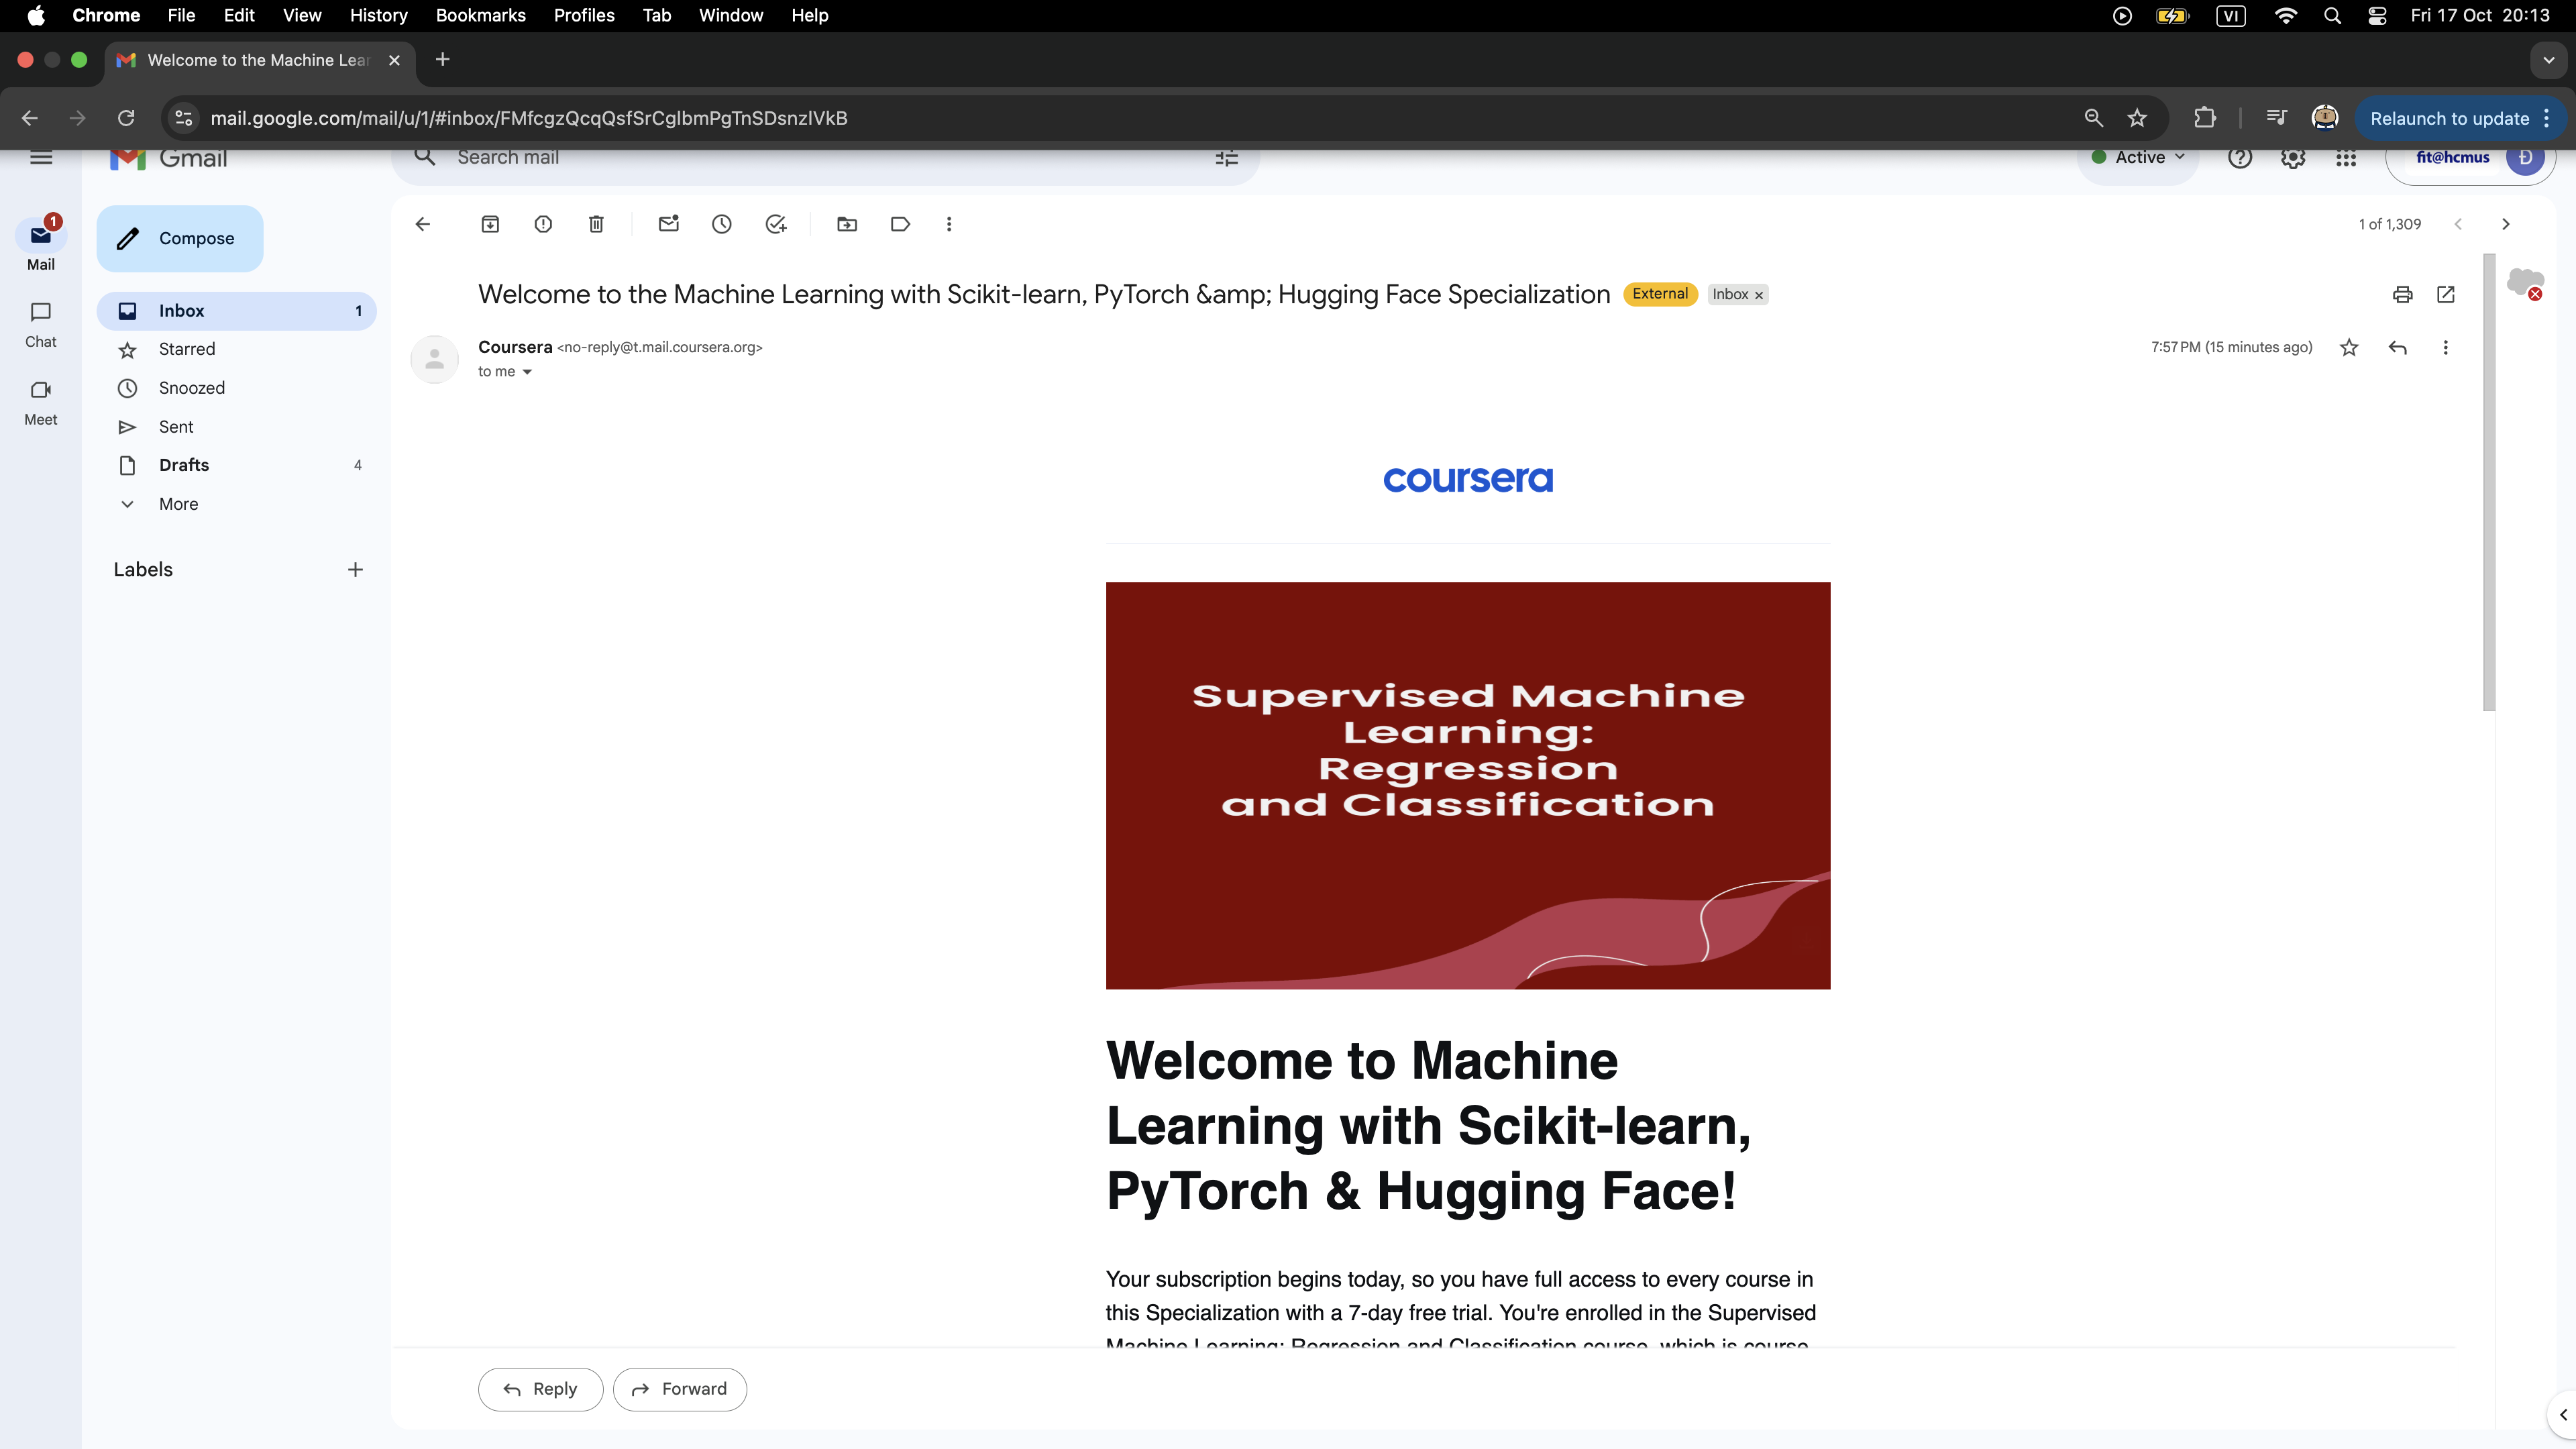
\includegraphics[scale=0.25]{Image/registration.png}
    \caption{Registration confirmation on Coursera (17/10/2025)}
\end{figure}
\section{Overview}

\subsection{Details of the Program}
%----------------------------------------

\indent\indent The \textbf{Machine Learning Specialization} is a foundational online program created in collaboration between \textbf{DeepLearning.AI} and \textbf{Stanford Online}. 
This beginner-friendly specialization teaches the fundamentals of machine learning and how to apply these techniques to build real-world AI applications.

This specialization is taught by \textbf{Andrew Ng}, an AI visionary who has led pioneering research at Stanford University and groundbreaking work at Google Brain, Baidu, and Landing.AI to advance the field of artificial intelligence.

This 3-course specialization is an updated version of Andrew Ng’s pioneering \emph{Machine Learning} course, rated 4.9 out of 5 and taken by over 4.8 million learners since it launched in 2012.

It provides a broad introduction to modern machine learning, including:
\begin{itemize}
    \item \textbf{Supervised Learning:} multiple linear regression, logistic regression, neural networks, and decision trees.
    \item \textbf{Unsupervised Learning:} clustering, dimensionality reduction, and recommender systems.
    \item \textbf{Best Practices:} evaluating and tuning models, and taking a data-centric approach to improving performance.
\end{itemize}

\noindent By the end of this specialization, learners will have mastered key concepts and gained the practical know-how to powerfully apply machine learning to challenging real-world problems. 
If you’re looking to break into AI or build a career in machine learning, this specialization is the ideal place to start.

\subsection{Projects in Specialization - 3 course series}

\begin{itemize}
    \item Build machine learning models in Python using popular machine learning libraries NumPy and scikit-learn.
    \item Build and train supervised machine learning models for prediction and binary classification tasks, including linear regression and logistic regression.
    \item Build and train a neural network with TensorFlow to perform multi-class classification.
    \item Apply best practices for machine learning development so that your models generalize to data and tasks in the real world.
    \item Build and use decision trees and tree ensemble methods, including random forests and boosted trees.
    \item Use unsupervised learning techniques for unsupervised learning: including clustering and anomaly detection.
    \item Build recommender systems with a collaborative filtering approach and a content-based deep learning method.
    \item Build a deep reinforcement learning model.
\end{itemize}
%----------------------------------------
\section{Supervised Machine Learning: Regression and Classification}
%----------------------------------------

This foundational course established the core principles of machine learning. It provided a comprehensive journey from the mathematical formulation of learning problems to the implementation of gradient-based optimization for both continuous (regression) and discrete (classification) prediction tasks.

\begin{figure}[H]
    \centering
    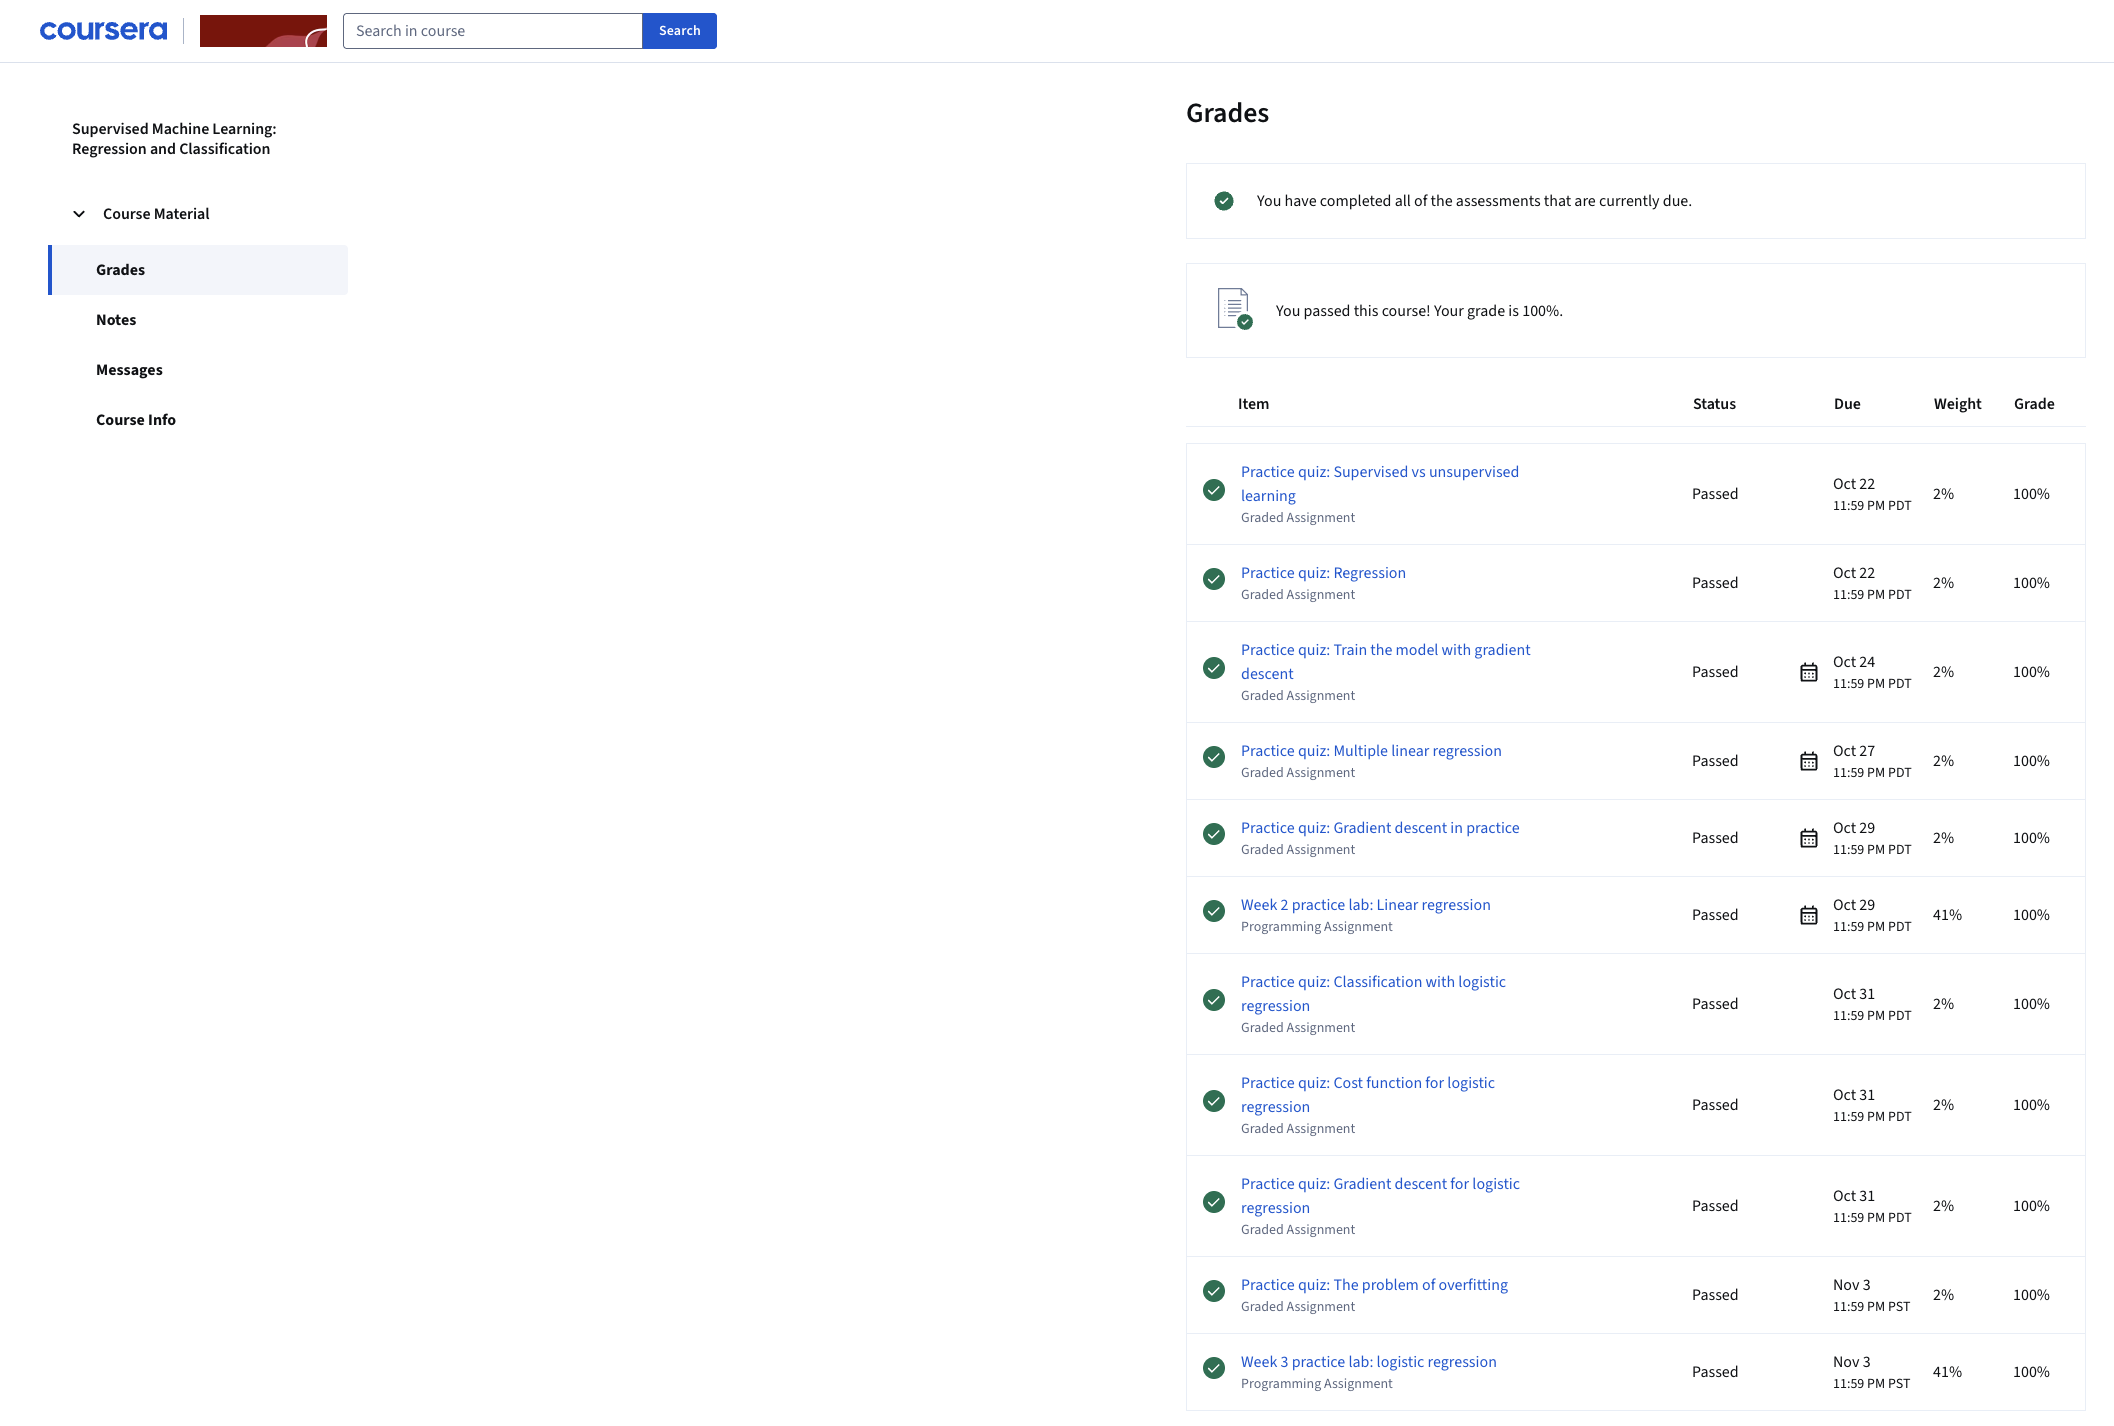
\includegraphics[scale=0.5]{Image/c1.png}
    \caption{Course 1 completed}
\end{figure}

%----------------------------------------
\subsection{Week 1: Introduction to Machine Learning}
%----------------------------------------

\subsubsection{Key Insights and Learnings}

This module introduced the fundamental paradigm shift from traditional programming to data-driven learning.

\begin{itemize}
    \item \textbf{The Supervised Learning Framework:} Structured the problem-solving approach around three core components:
    \begin{enumerate}
        \item \textbf{Model Representation:} Mathematically defined the relationship between inputs $x$ and output $y$ (e.g., Linear Regression $f_{w,b}(x) = wx + b$).
        \item \textbf{Cost Function ($J$):} Quantified the model's error. For regression, the \textbf{Mean Squared Error (MSE)} is used to measure the average squared difference between predictions and actual targets.
        \item \textbf{Gradient Descent Optimization:} Implemented an iterative algorithm that updates parameters ($w, b$) by moving against the gradient of the cost function ($\alpha \frac{\partial J}{\partial w}$) to reach the global minimum.
    \end{enumerate}

    \item \textbf{Learning Paradigms:}
    \begin{itemize}
        \item \textbf{Supervised Learning:} Training models on labeled data (Input $X$ $\rightarrow$ Output $Y$) to predict future outcomes.
        \item \textbf{Unsupervised Learning:} Extracting hidden structures or clusters from unlabeled data (explored deeply in later courses).
    \end{itemize}
\end{itemize}

\subsubsection{Learning Evidence}
\begin{figure}[H]
    \centering
    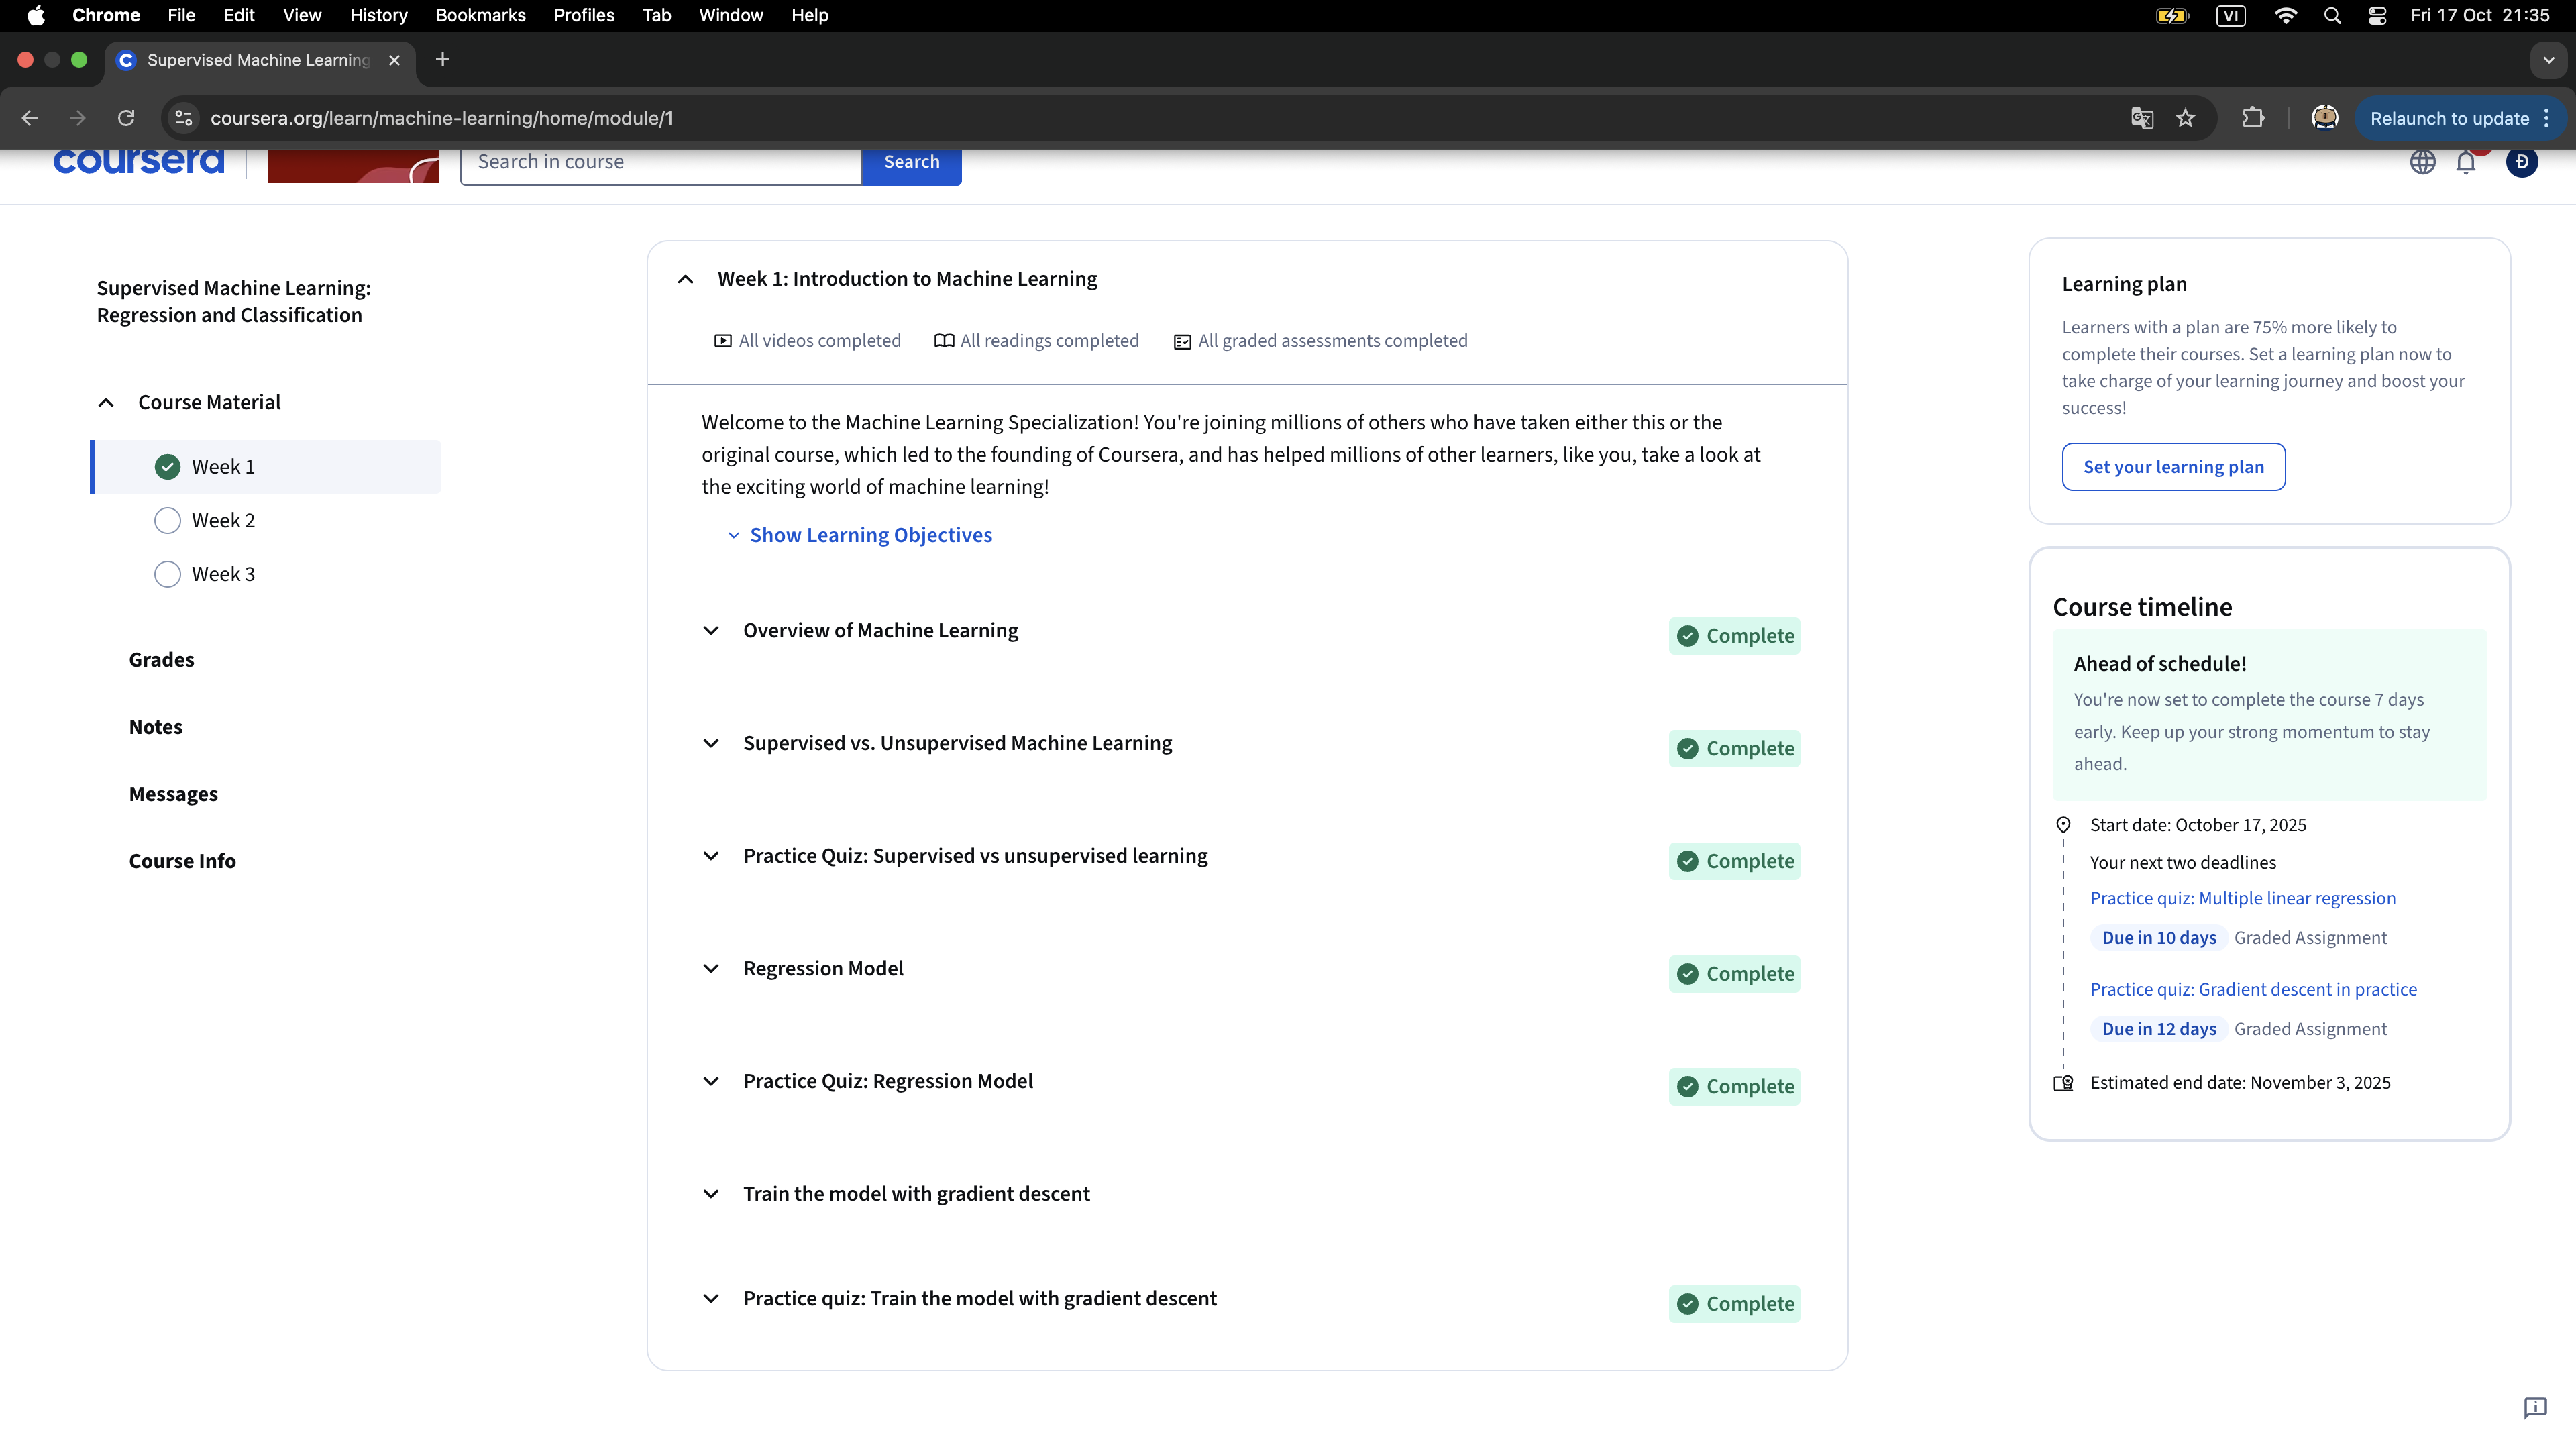
\includegraphics[scale=0.25]{Image/c1_w1.png}
    \caption{Lesson's completed date (17/10/2025)}
\end{figure}

\subsubsection{Graded Assignment Evidence}
\begin{figure}[H]
    \centering
    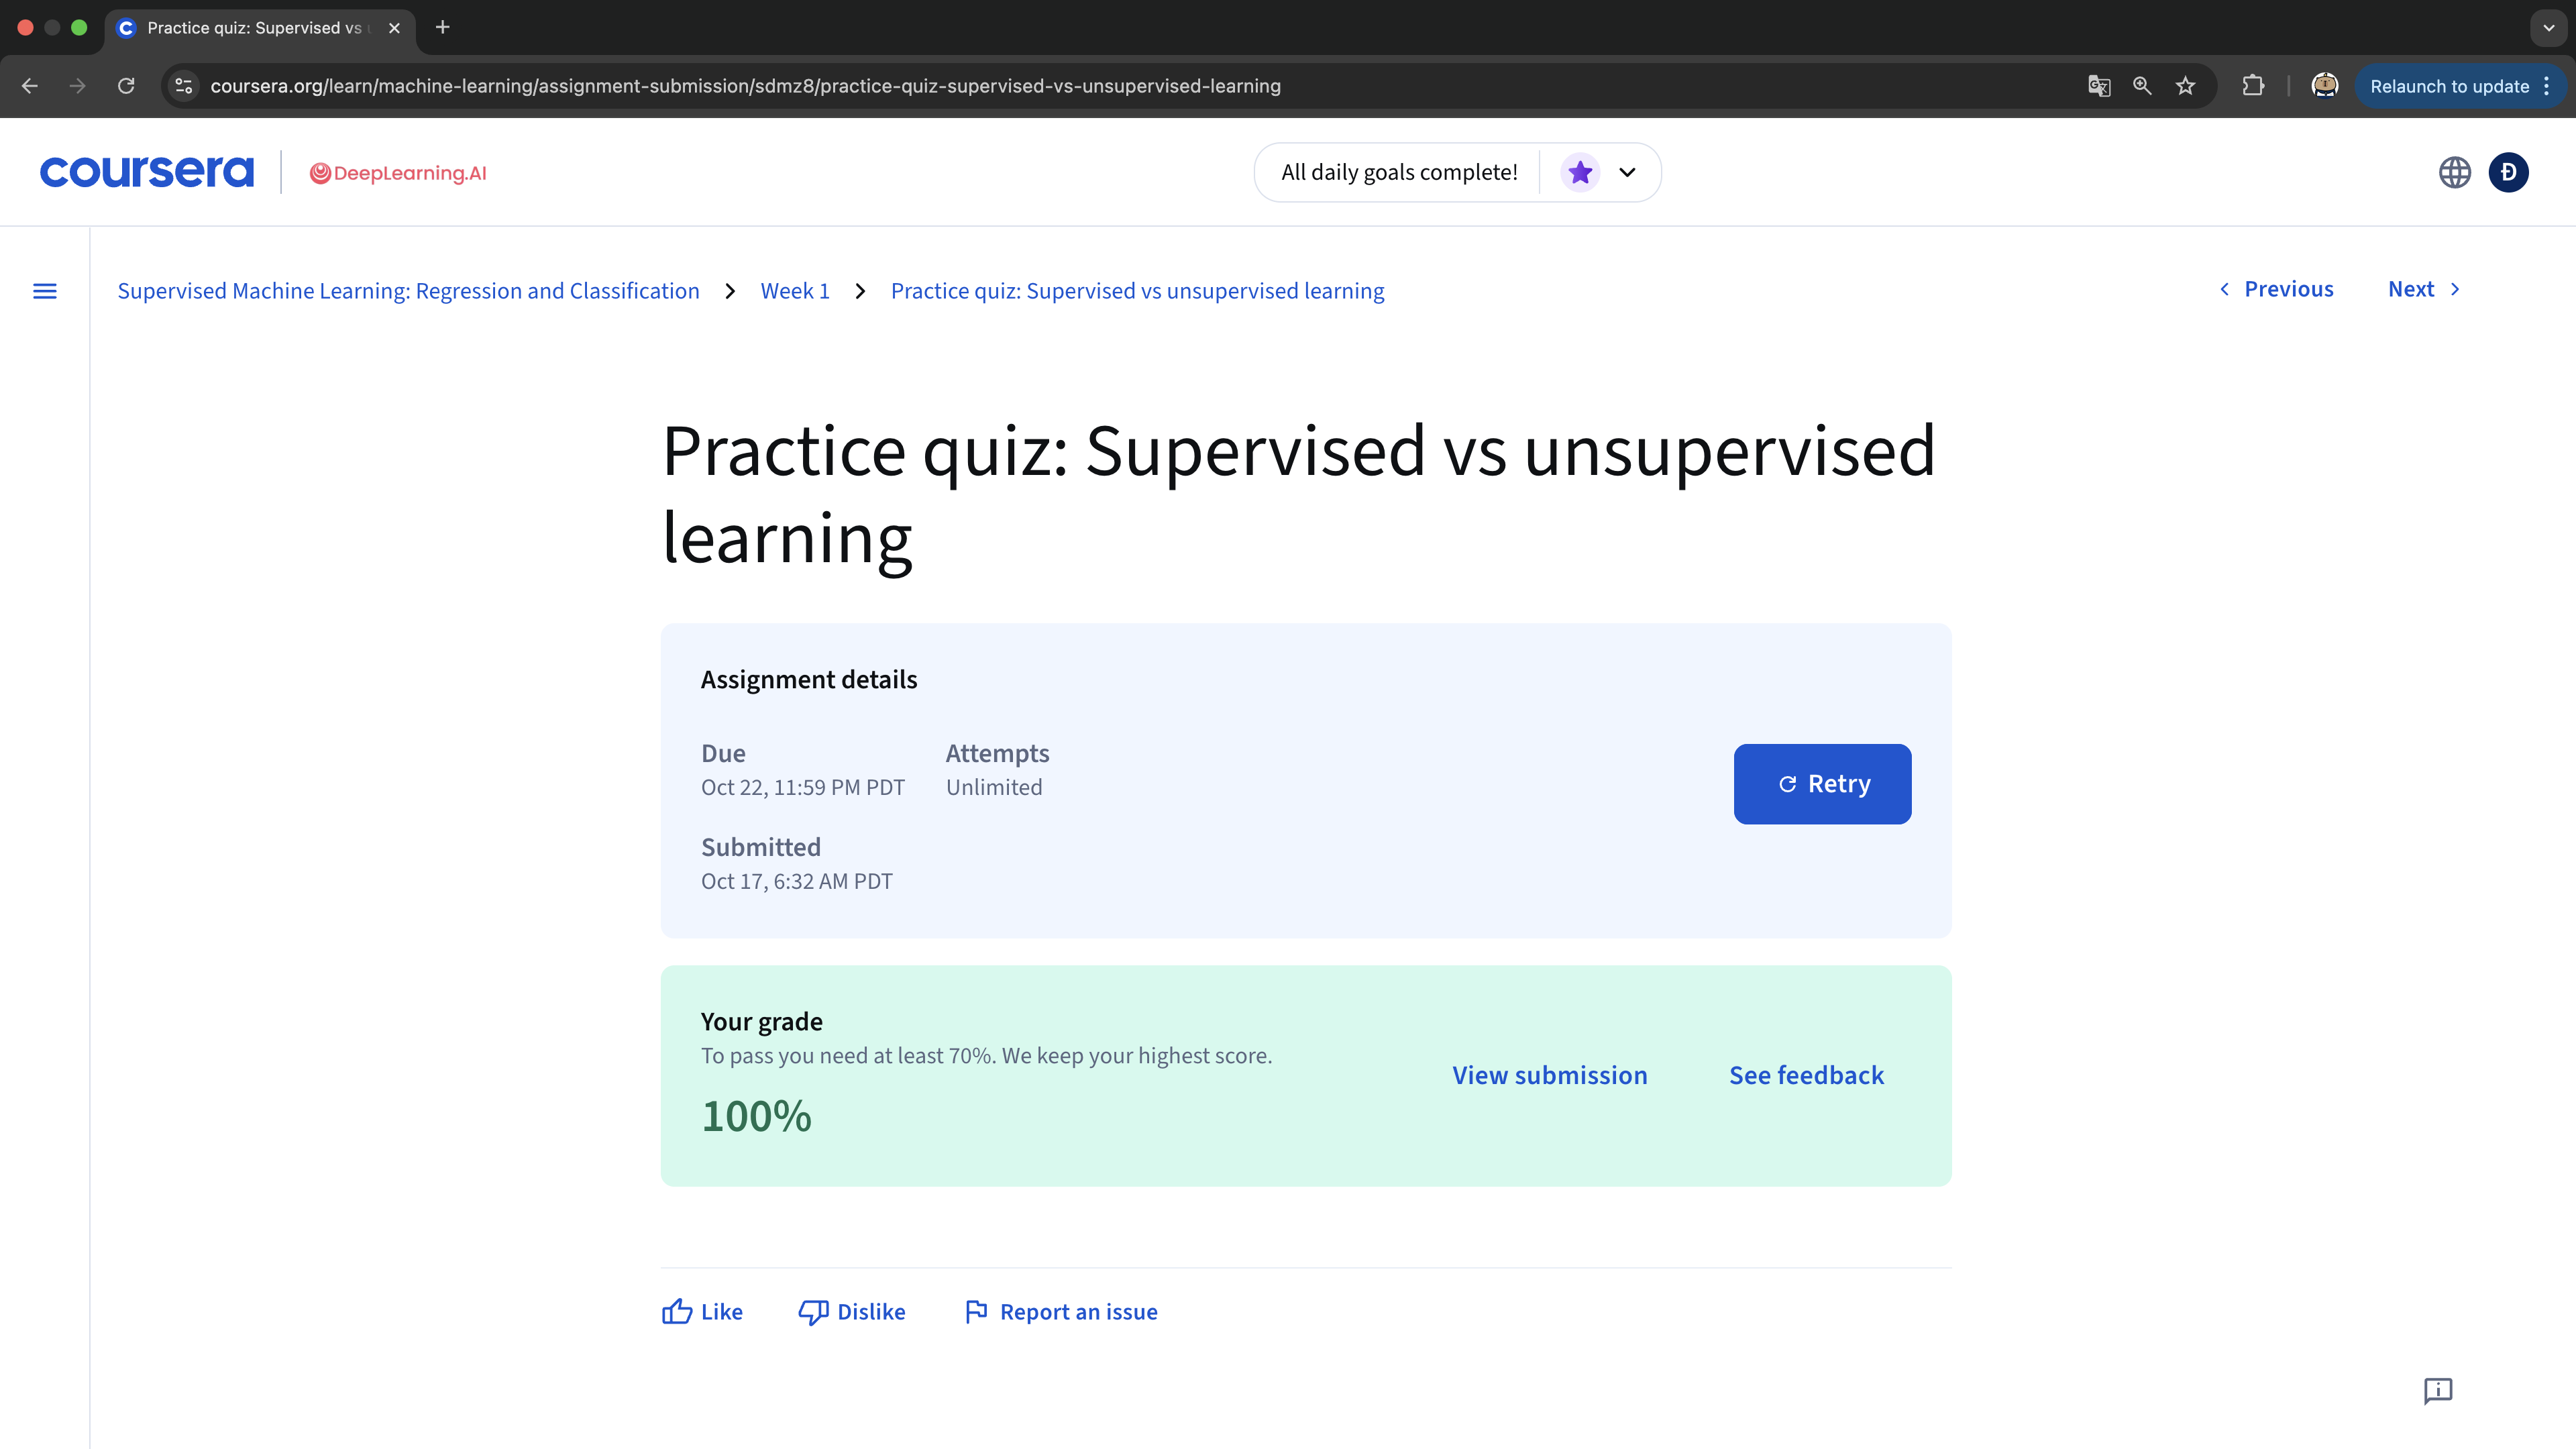
\includegraphics[scale=0.25]{Image/c1_w1_q1.png}
    \caption{Completed Graded Assignment 1 (Supervised vs unsupervised learning)}
\end{figure}

\begin{figure}[H]
    \centering
    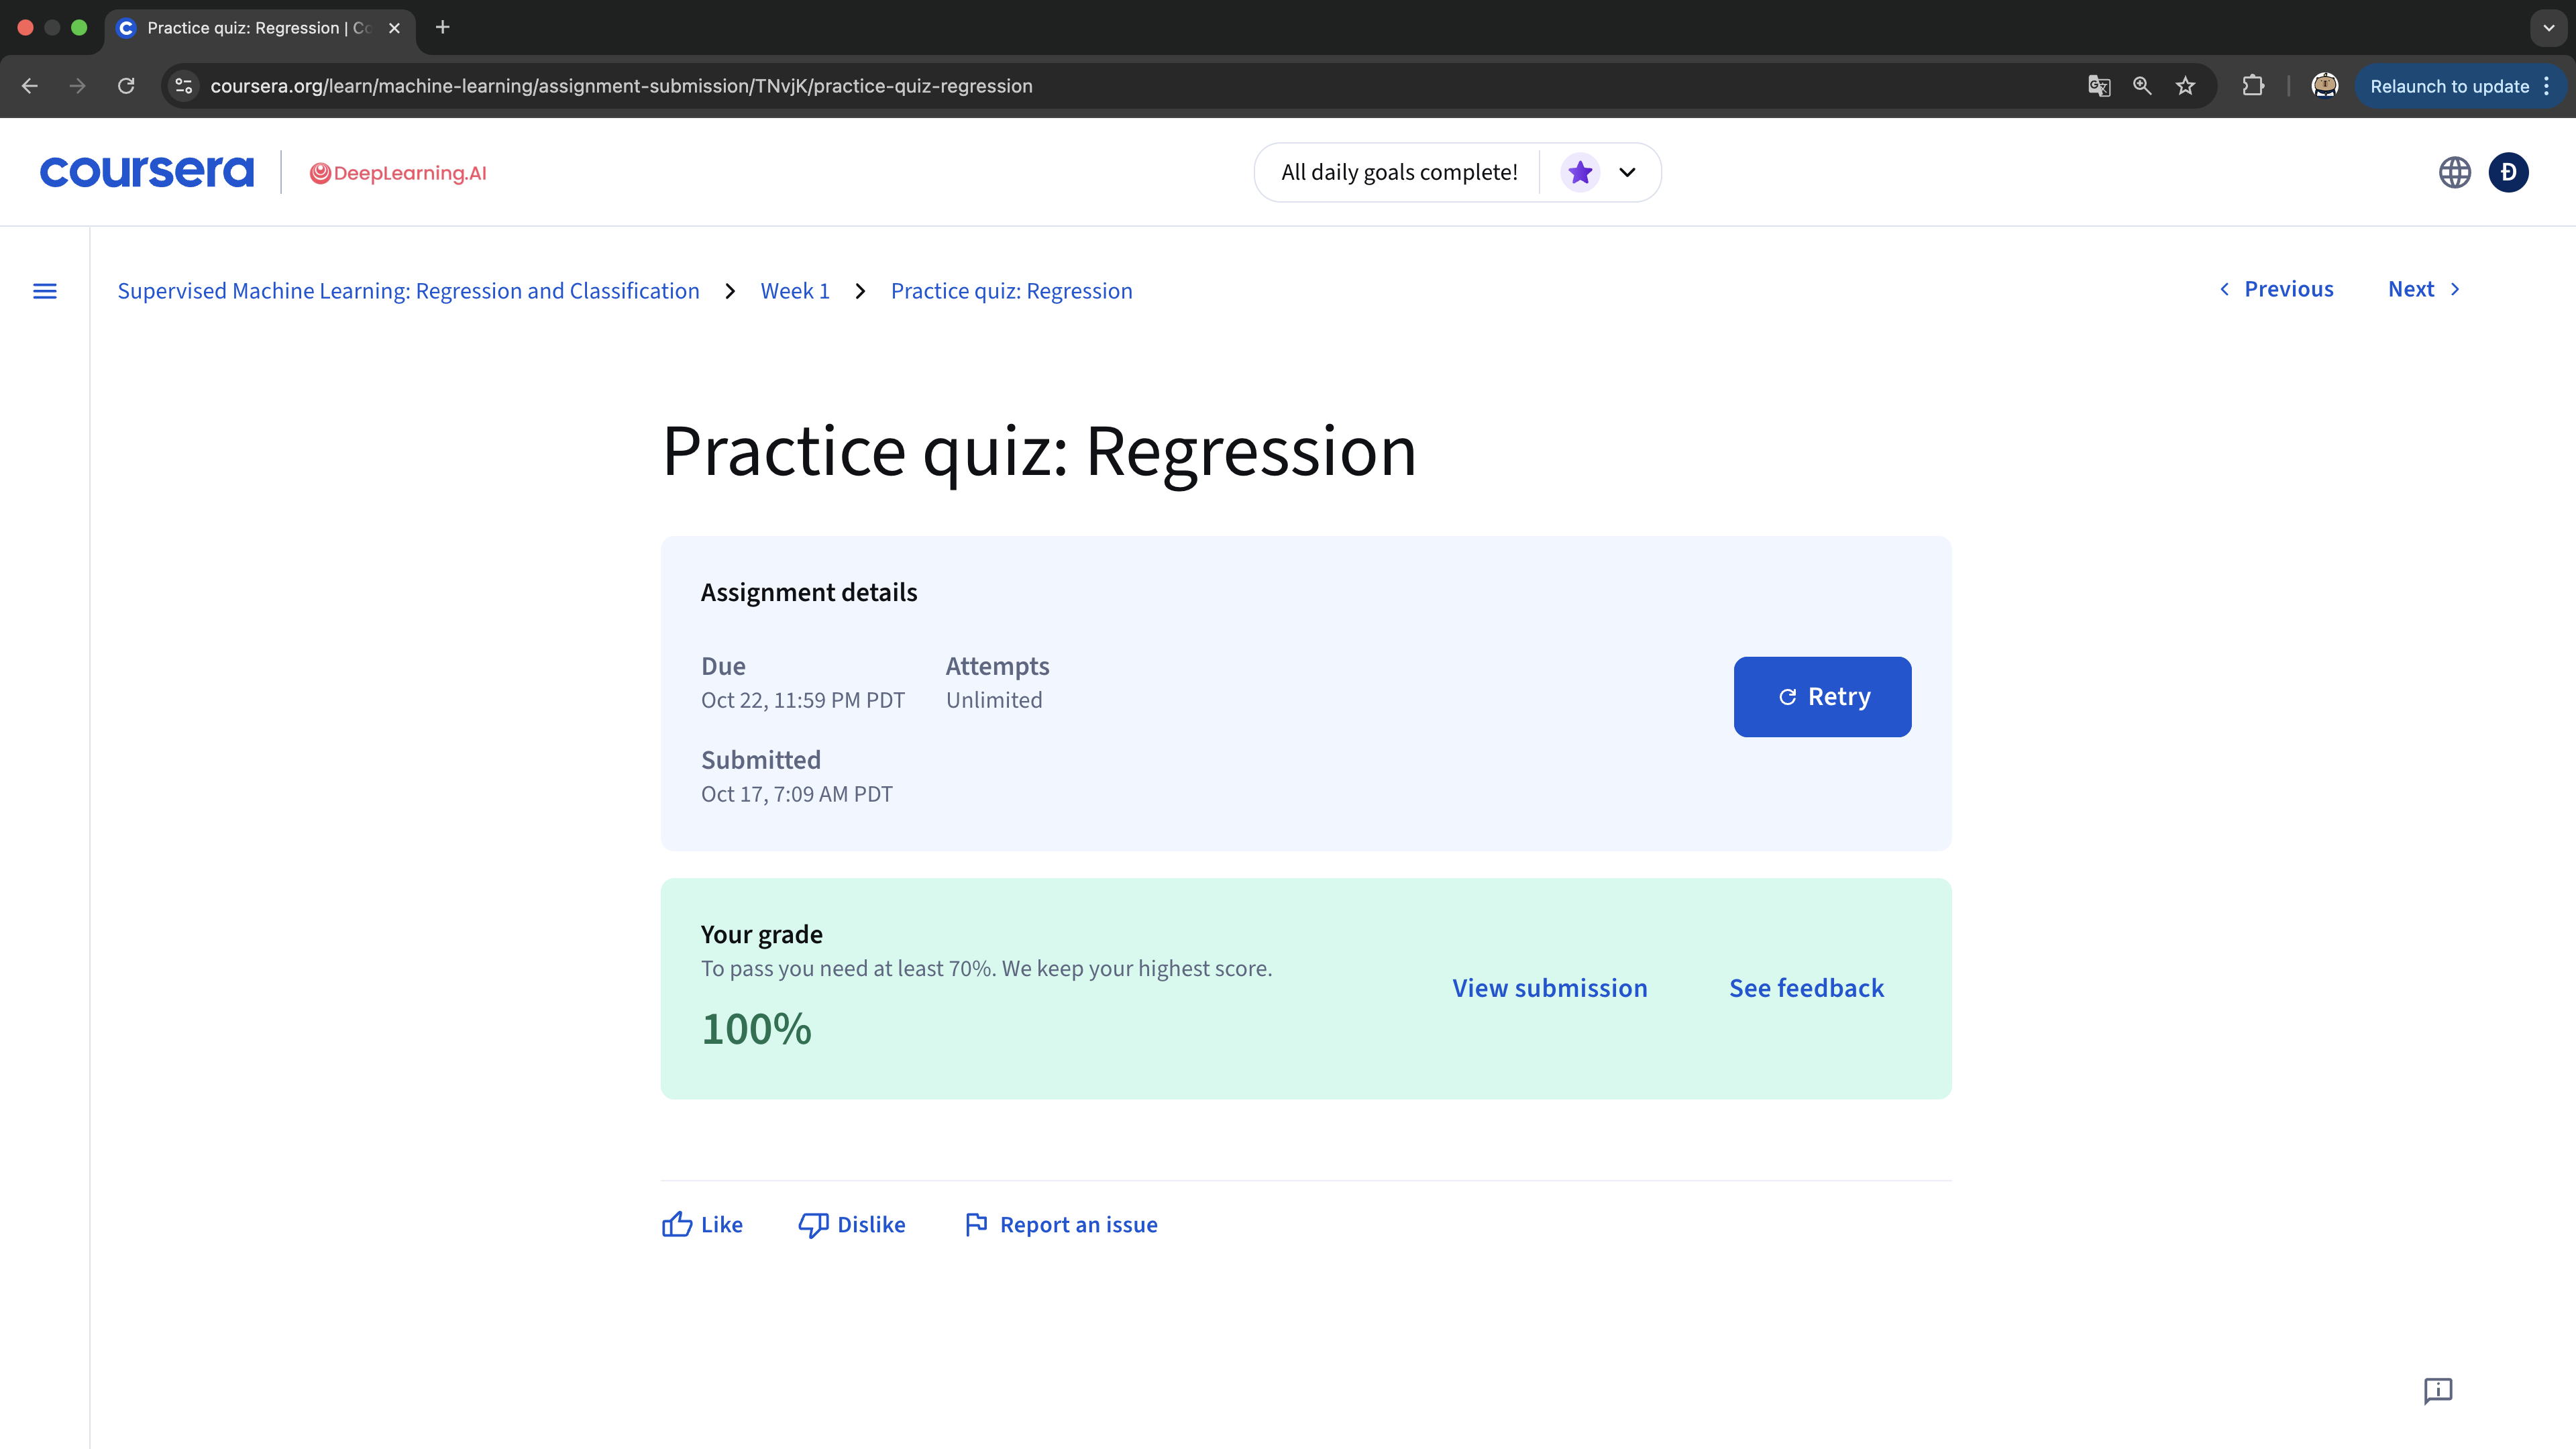
\includegraphics[scale=0.25]{Image/c1_w1_q2.png}
    \caption{Completed Graded Assignment 2 (Regression)}
\end{figure}

\begin{figure}[H]
    \centering
    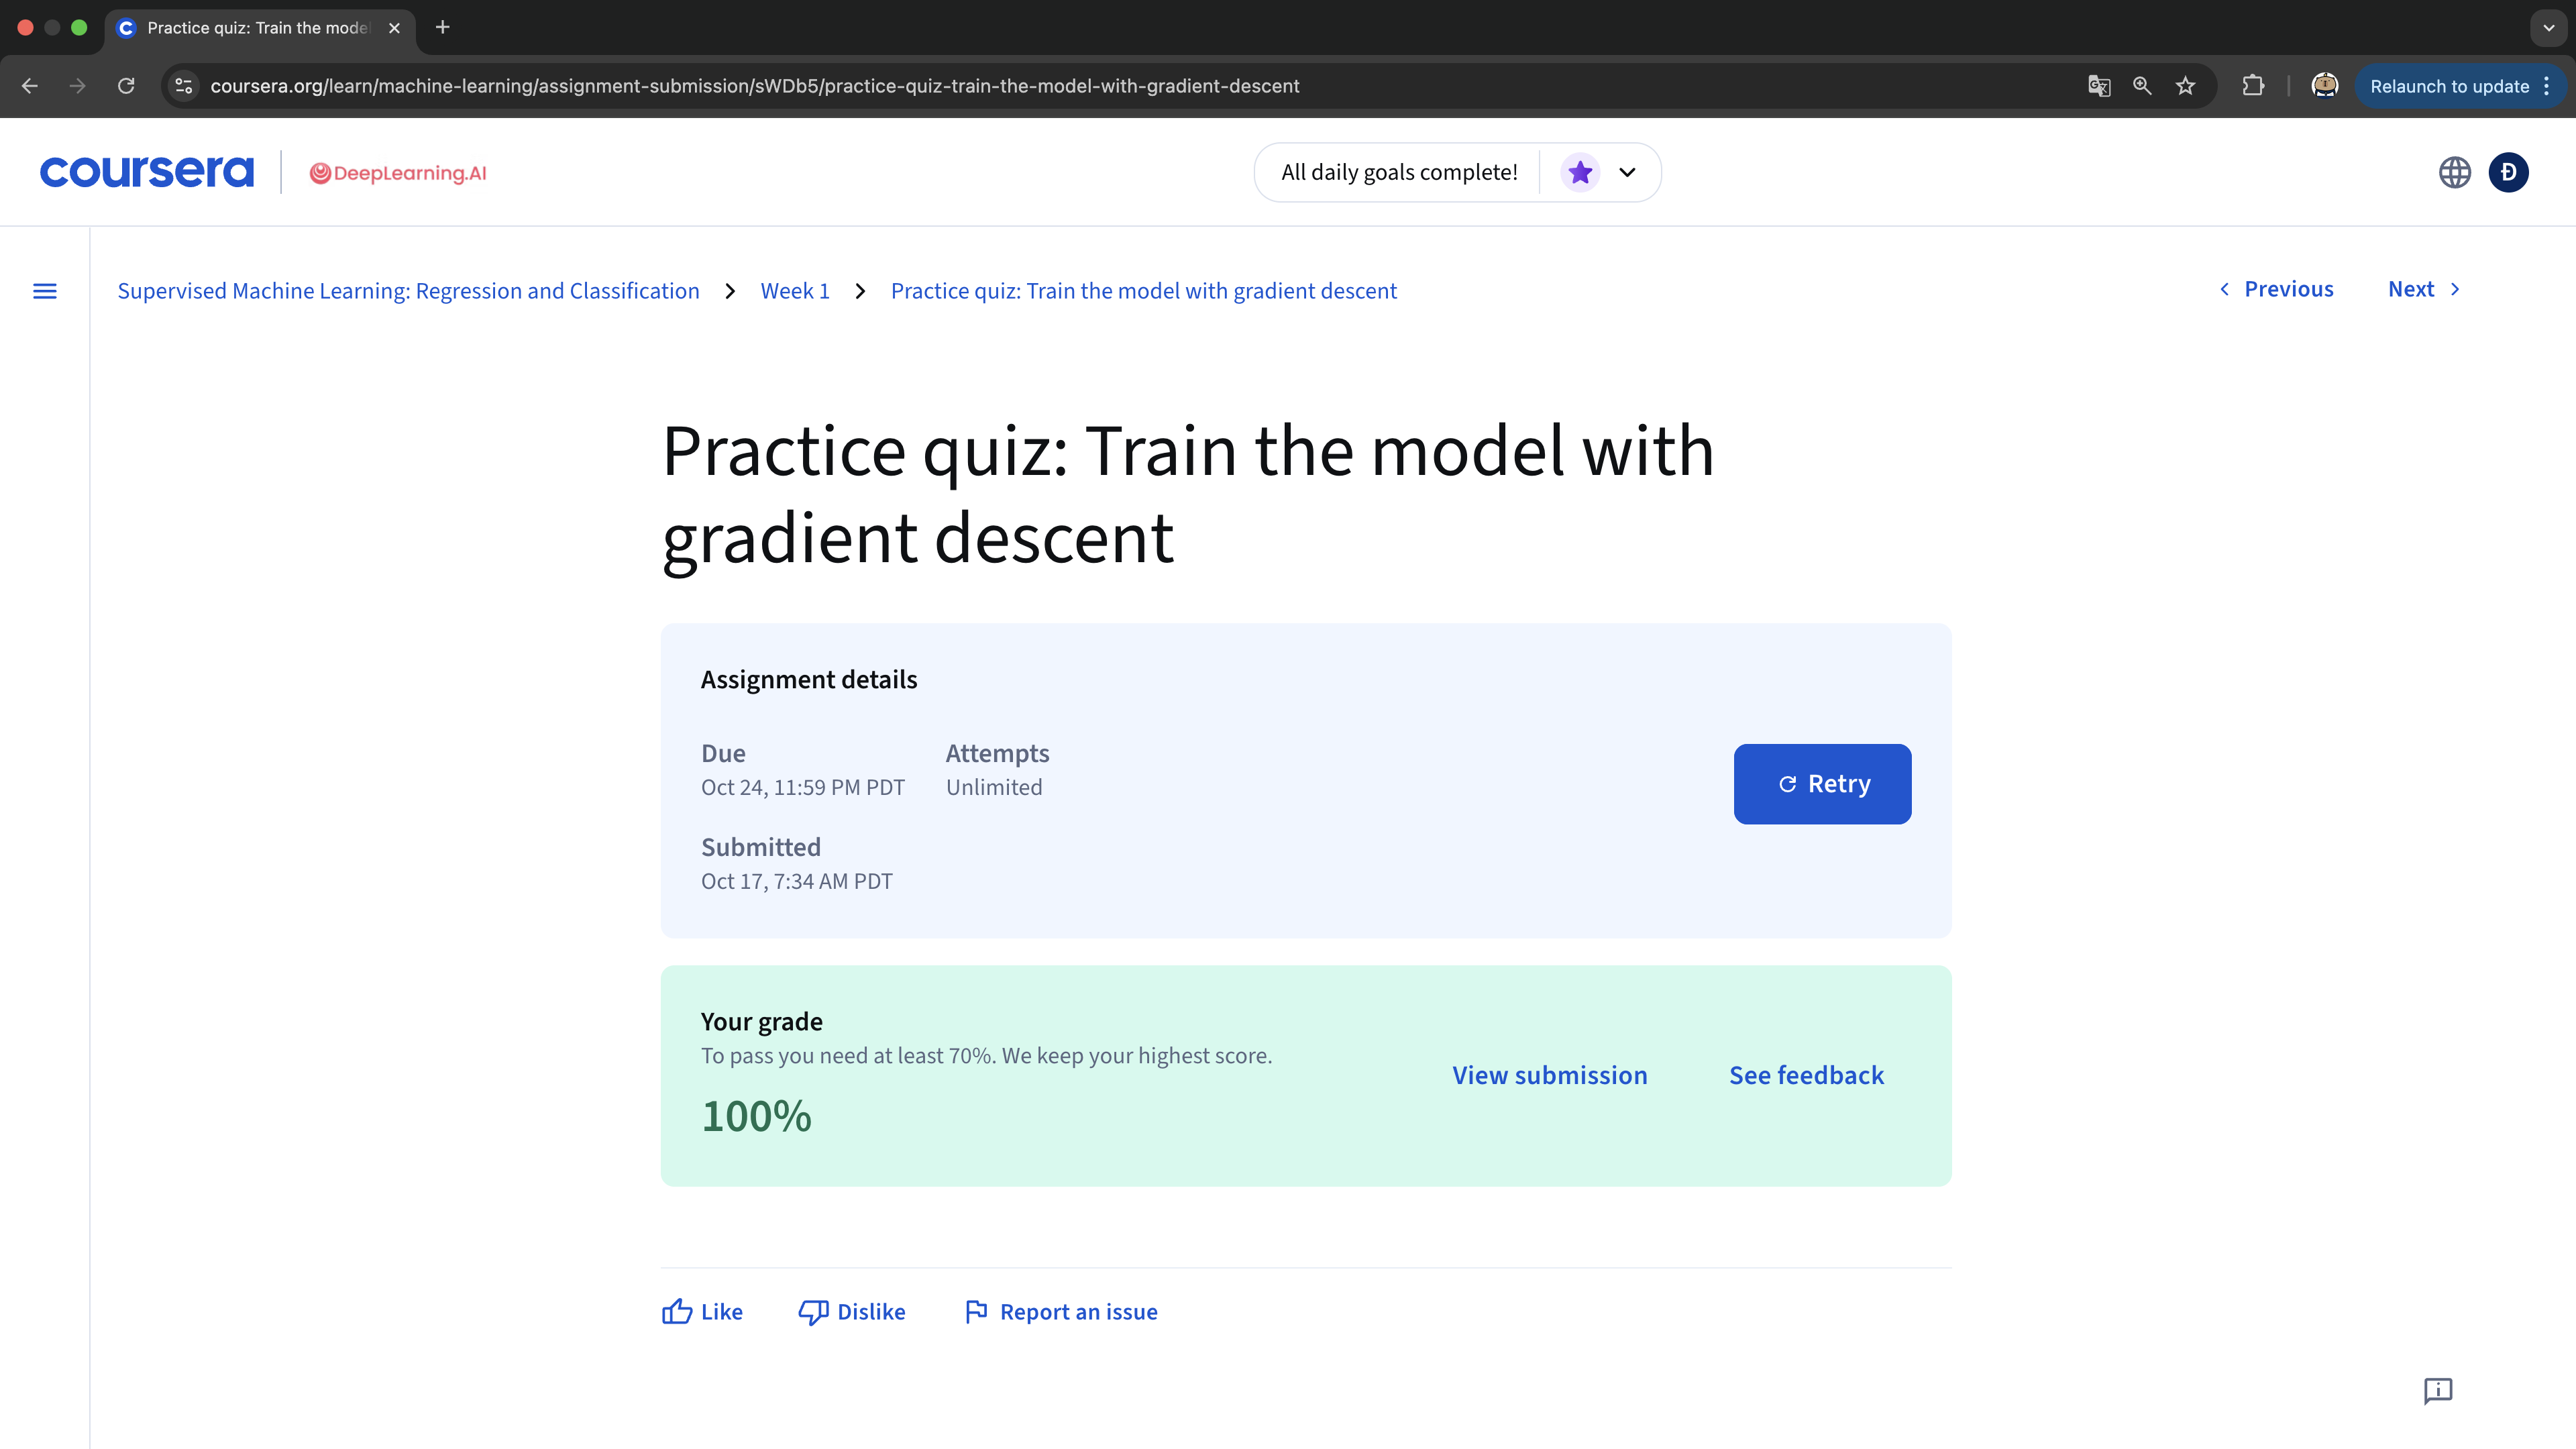
\includegraphics[scale=0.25]{Image/c1_w1_q3.png}
    \caption{Completed Graded Assignment 3 (Train the model with gradient descent)}
\end{figure}

%----------------------------------------
\subsection{Week 2: Regression with Multiple Input Variables}
%----------------------------------------

\subsubsection{Key Insights and Learnings}

This module expanded linear regression to handle complex, real-world datasets with multiple features, focusing on computational efficiency and convergence speed.

\begin{itemize}
    \item \textbf{Vectorization (NumPy):} Leveraged linear algebra principles to process large datasets. By replacing explicit \texttt{for} loops with vector/matrix operations ($np.dot$), computation time is drastically reduced, enabling the training of scalable models.

    \item \textbf{Feature Scaling \& Convergence:}
    \begin{itemize}
        \item \textbf{Problem:} When features have vastly different scales (e.g., price vs. number of bedrooms), the cost function contours become elongated (elliptical), causing Gradient Descent to oscillate and converge slowly.
        \item \textbf{Solution:} Applied \textbf{Z-score Normalization} to rescale features. This transforms the cost function contours into circles, allowing Gradient Descent to take a direct path to the minimum.
    \end{itemize}

    \item \textbf{Feature Engineering and Polynomial Regression:} Learned that model power isn't limited by linear features. By engineering new features (e.g., $x^2, x^3, \sqrt{x}$), a linear model can be adapted to fit non-linear curves, enhancing flexibility without changing the underlying optimization algorithm.
\end{itemize}

\subsubsection{Learning Evidence}
\begin{figure}[H]
    \centering
    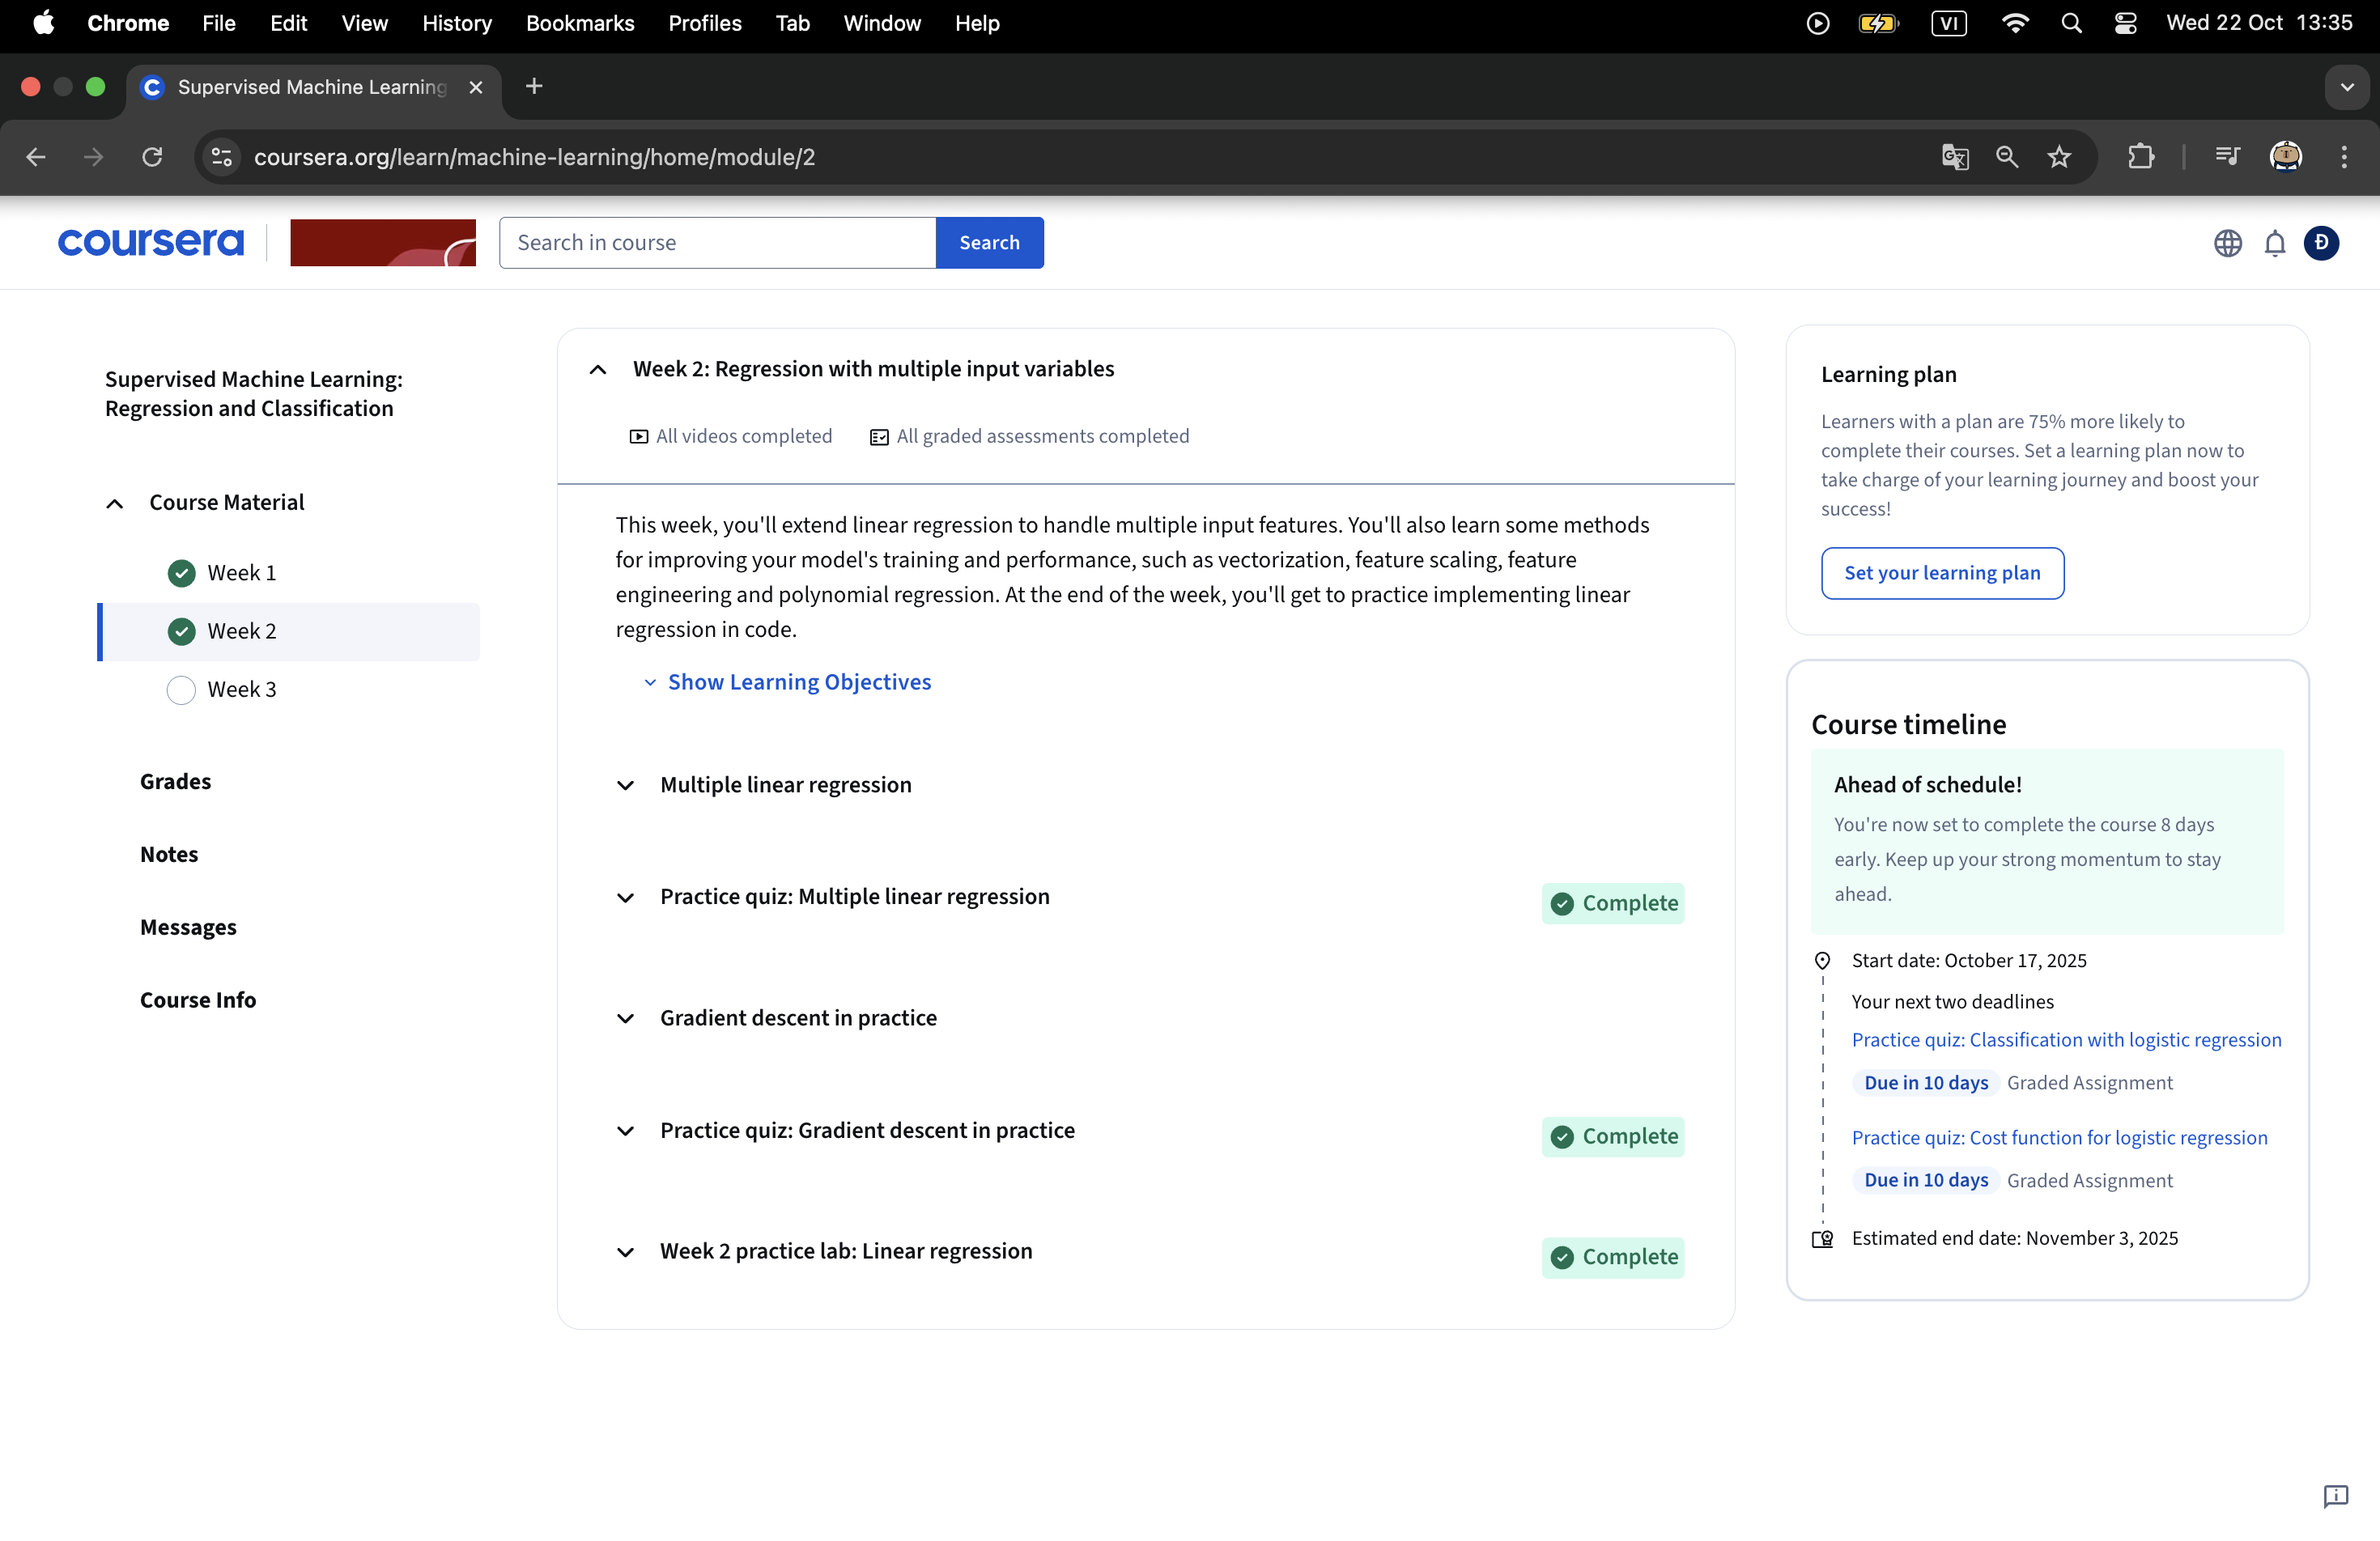
\includegraphics[scale=0.25]{Image/c1_w2.png}
    \caption{Lesson's completed date (22/10/2025)}
\end{figure}

\subsubsection{Graded Assignment Evidence}
\begin{figure}[H]
    \centering
    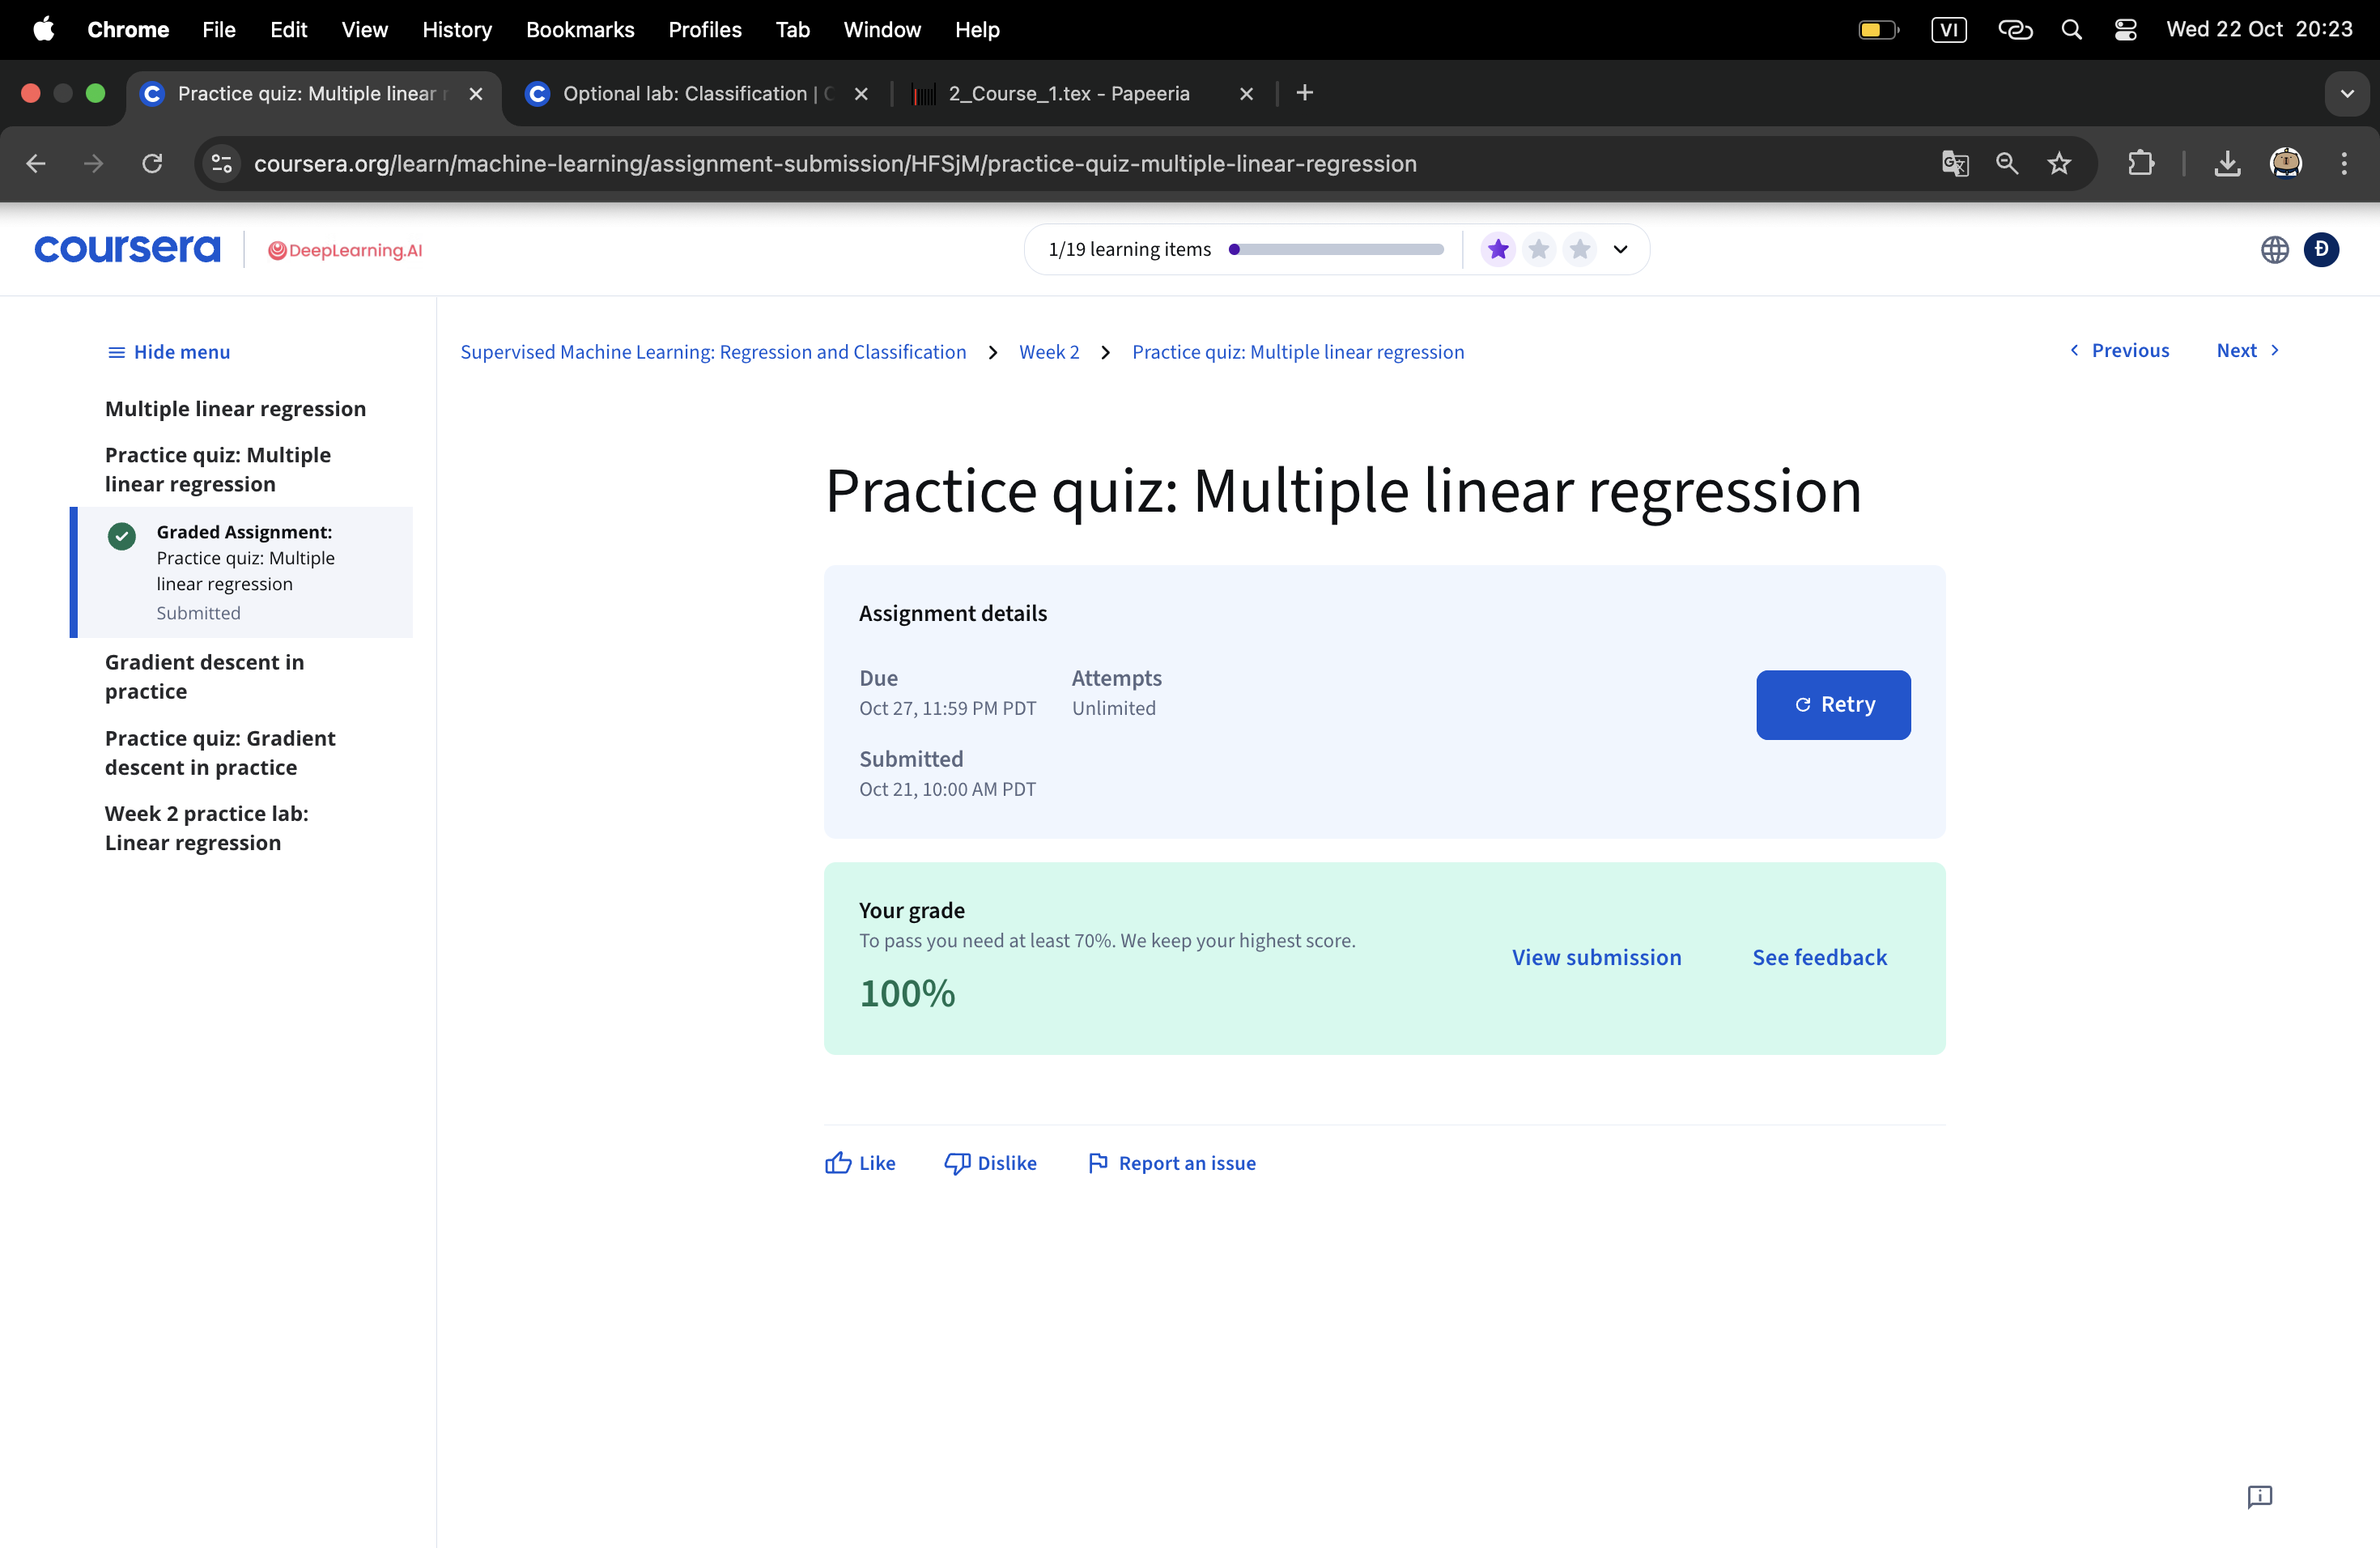
\includegraphics[scale=0.25]{Image/c1_w2_q1.png}
    \caption{Completed Graded Assignment 1 (Multiple linear regression)}
\end{figure}

\begin{figure}[H]
    \centering
    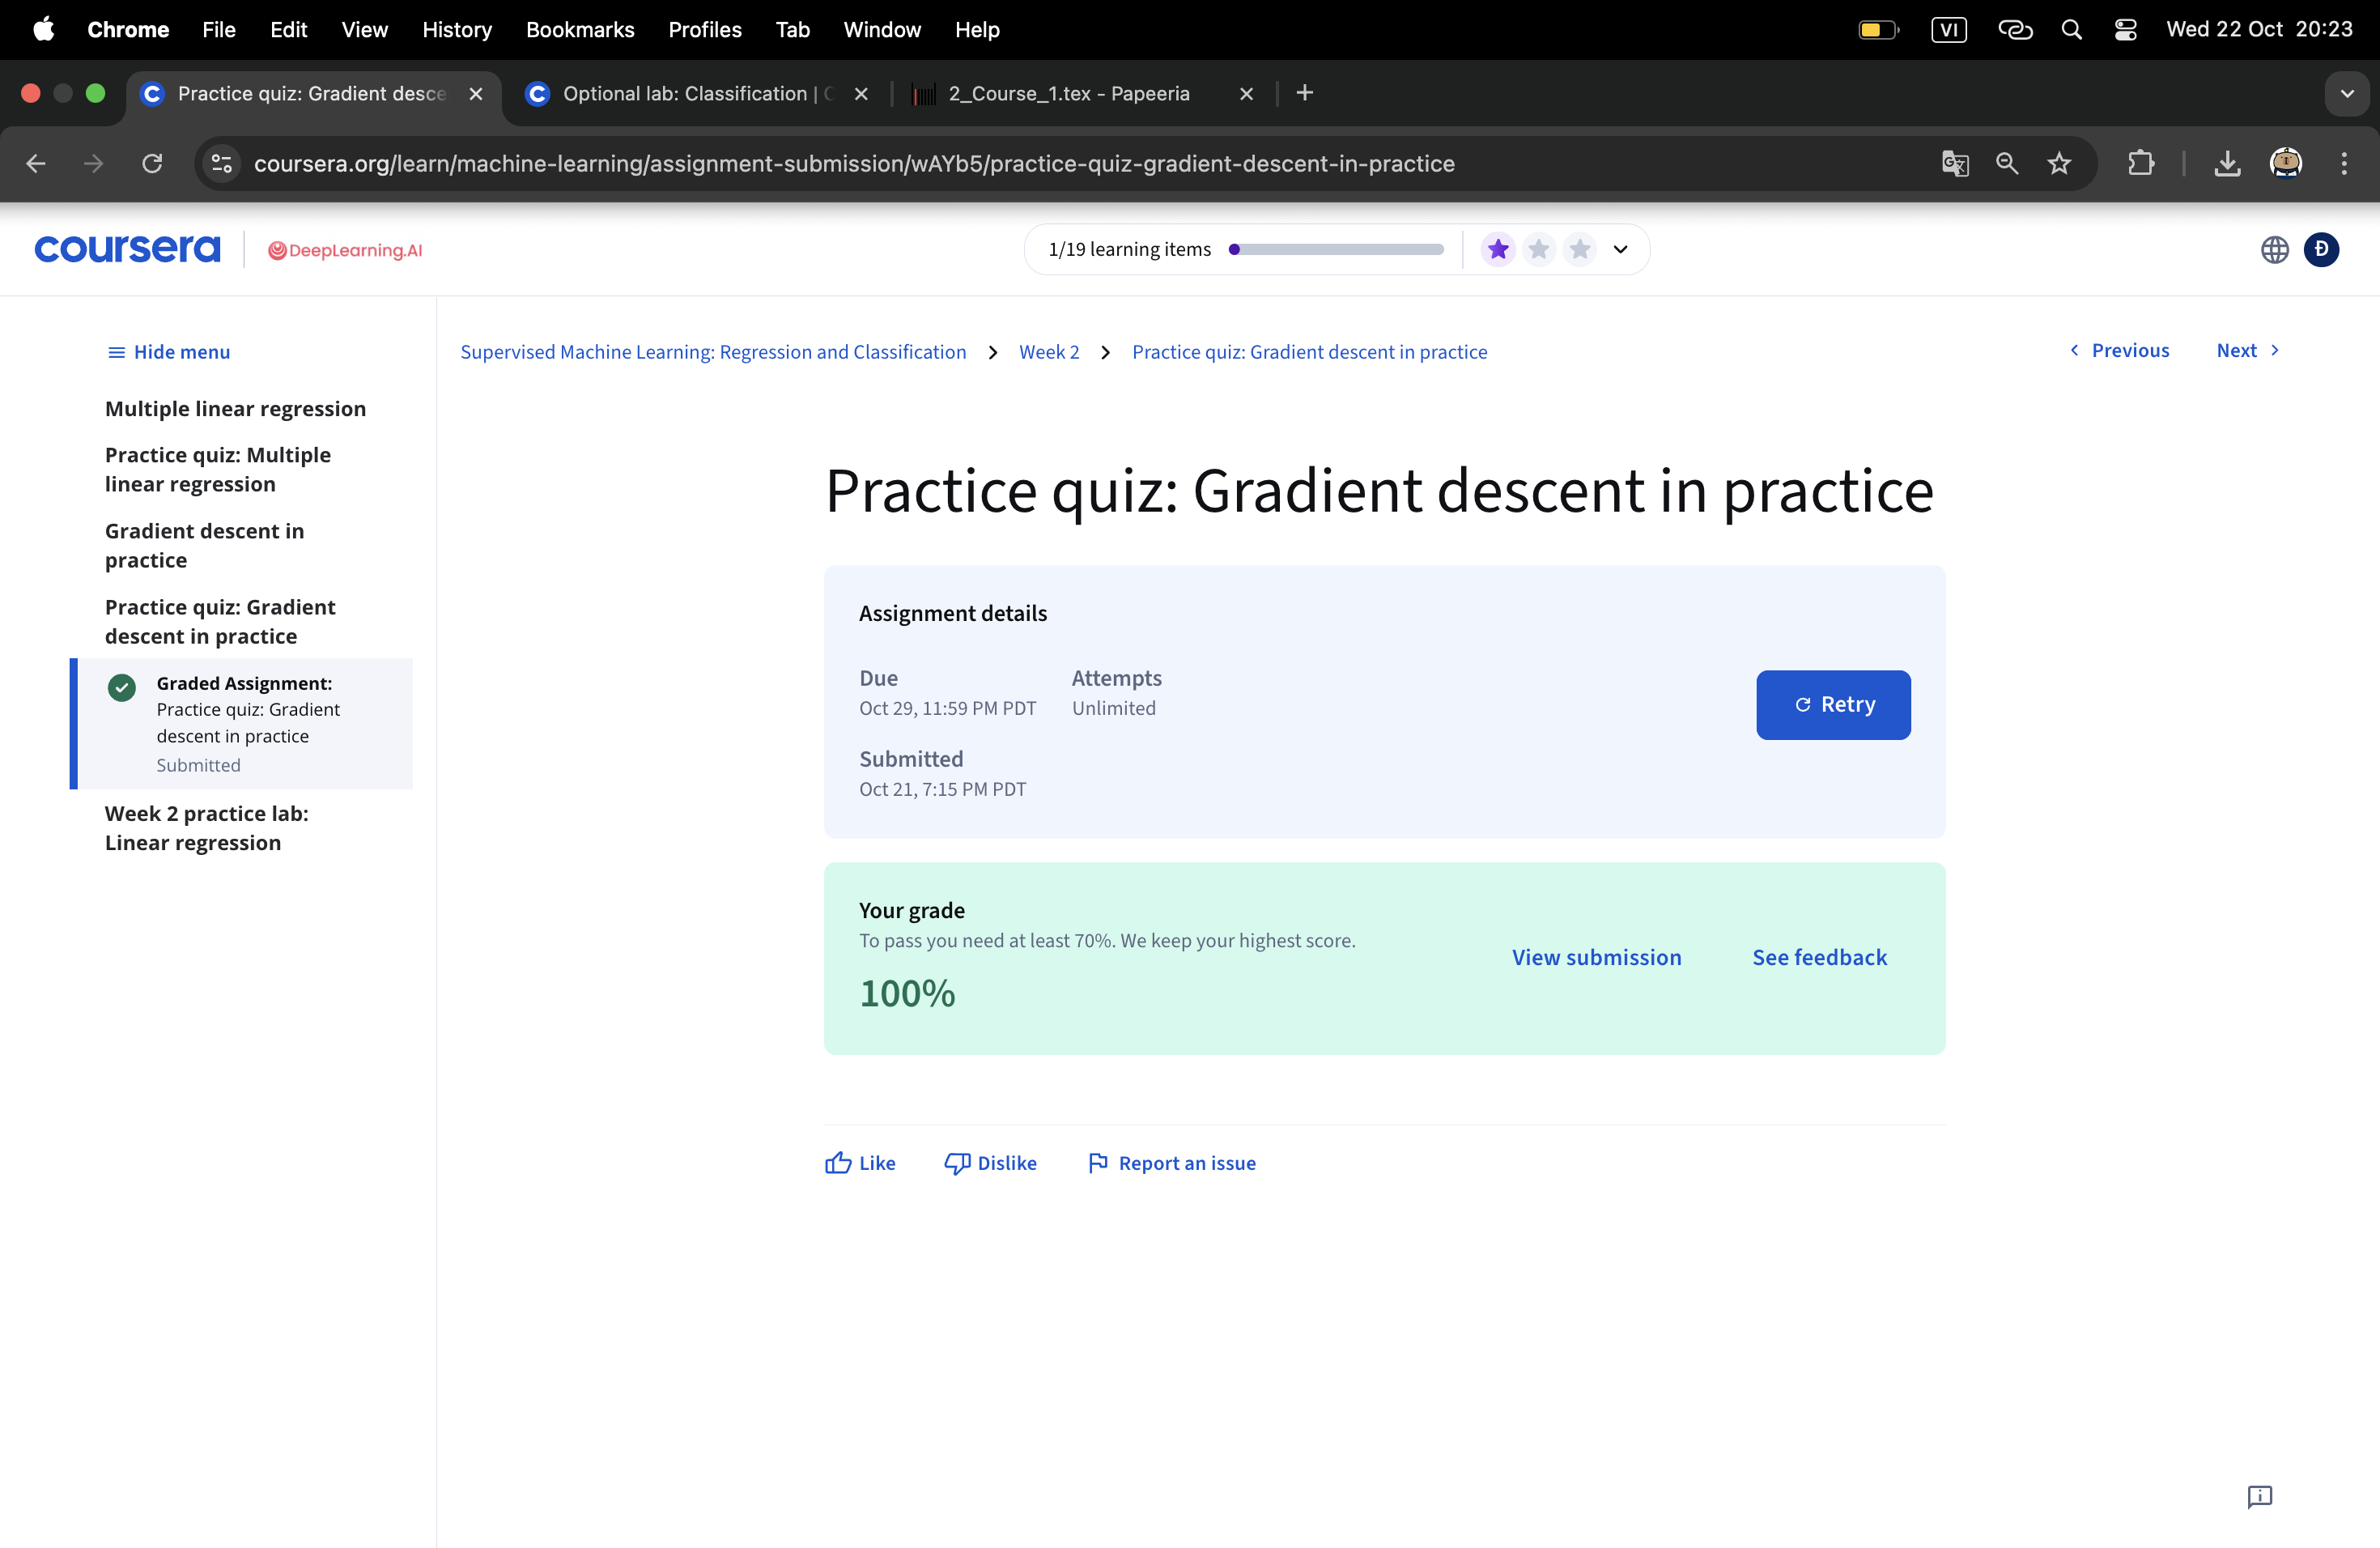
\includegraphics[scale=0.25]{Image/c1_w2_q2.png}
    \caption{Completed Graded Assignment 2 (Gradient descent in practice)}
\end{figure}

\begin{figure}[H]
    \centering
    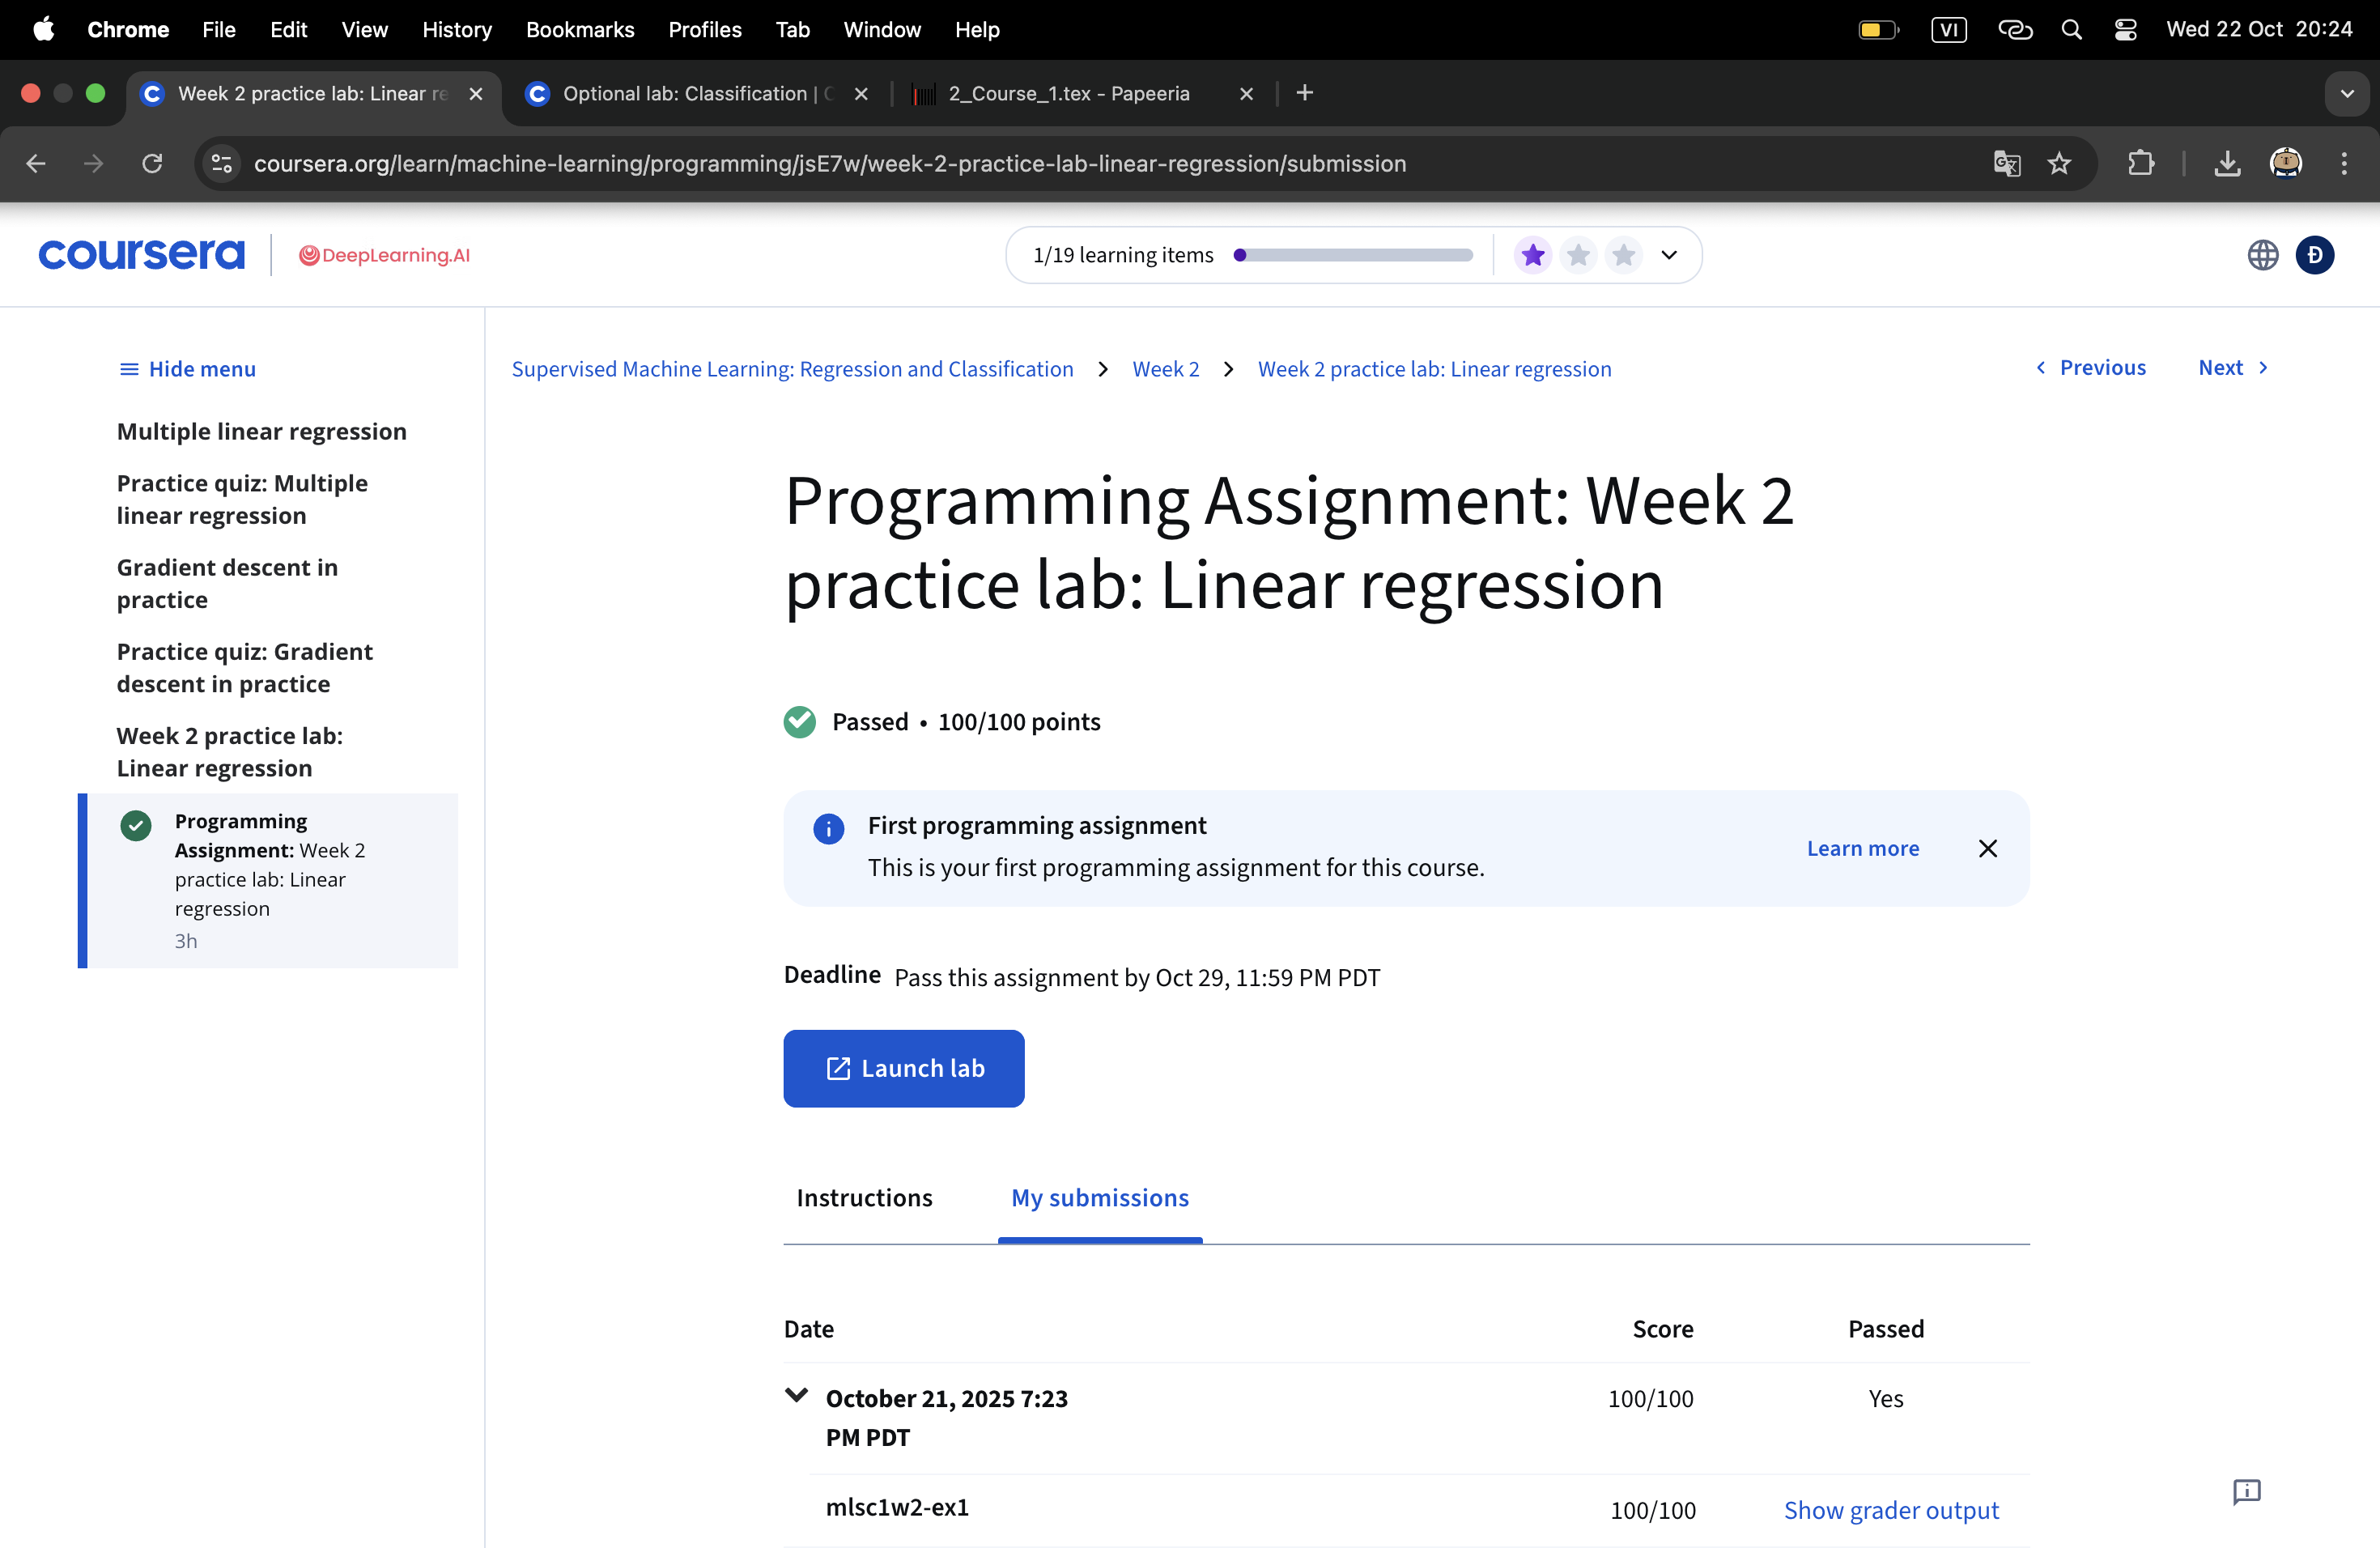
\includegraphics[scale=0.25]{Image/c1_w2_q3.png}
    \caption{Completed Programming Assignment (Linear regression)}
\end{figure}

%----------------------------------------
\subsection{Week 3: Classification}
%----------------------------------------

\subsubsection{Key Insights and Learnings}

This module introduced the mathematical adaptations required to predict categories rather than continuous numbers.

\begin{itemize}
    \item \textbf{Logistic Regression and The Sigmoid Function:} 
    \begin{itemize}
        \item Addressed the limitations of linear regression for classification (unbounded output).
        \item Applied the \textbf{Sigmoid Function} ($g(z) = \frac{1}{1+e^{-z}}$) to map predictions to a probability range $[0, 1]$, interpreting the output as $P(y=1|x)$.
    \end{itemize}

    \item \textbf{Decision Boundaries:} Visualized classification not just as a prediction task, but as finding a geometric boundary (line or polynomial curve) that separates different classes in the feature space.

    \item \textbf{The Logistic Loss Function:} 
    \begin{itemize}
        \item Learned that using MSE for Logistic Regression results in a \textbf{non-convex} cost function (many local minima).
        \item Implemented the \textbf{Log Loss (Binary Cross-Entropy)} function to ensure the cost function is convex, guaranteeing that Gradient Descent can find the global optimum.
    \end{itemize}

    \item \textbf{Overfitting and Regularization:} 
    \begin{itemize}
        \item \textbf{The Problem:} Models that fit training data too closely (high variance) fail to generalize to new data.
        \item \textbf{The Solution:} Implemented \textbf{L2 Regularization}. By adding a penalty term ($\lambda \sum w_j^2$) to the cost function, the model is forced to keep weights small, resulting in a simpler, smoother decision boundary that generalizes better.
    \end{itemize}
\end{itemize}

\subsubsection{Learning Evidence}
\begin{figure}[H]
    \centering
    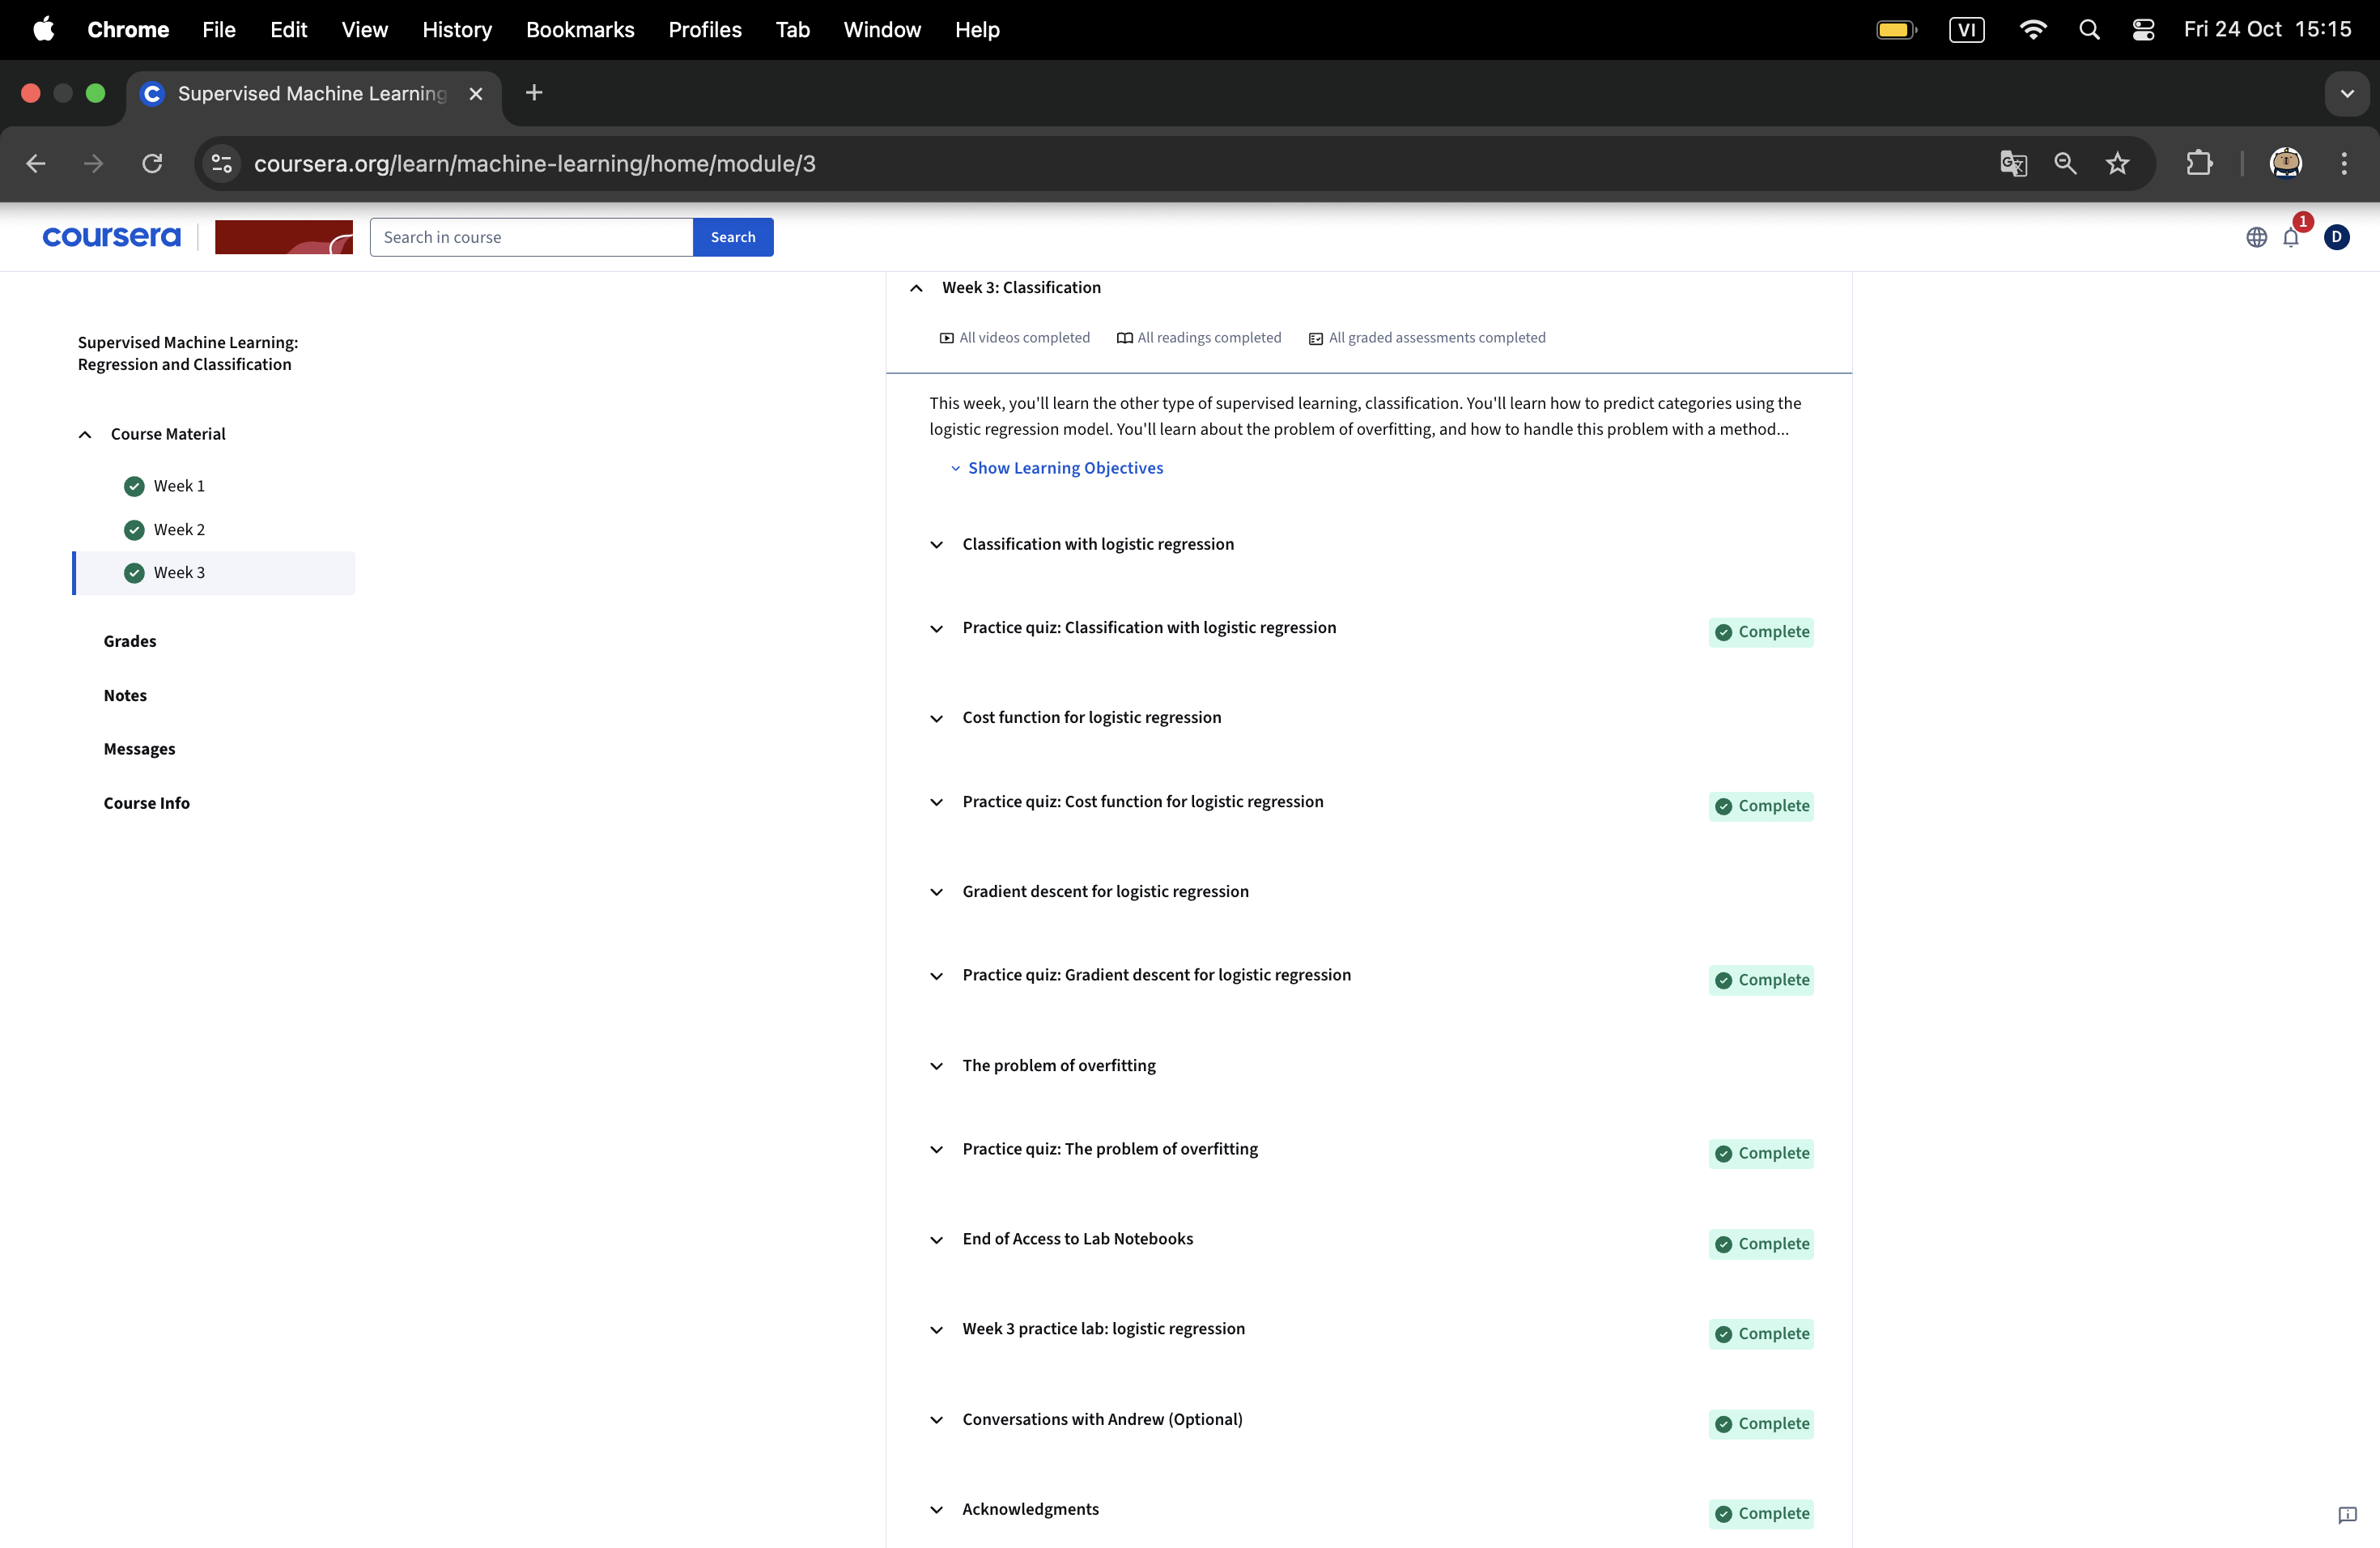
\includegraphics[scale=0.25]{Image/c1_w3.png}
    \caption{Lesson's completed date (24/10/2025)}
\end{figure}

\subsubsection{Graded Assignment Evidence}
\begin{figure}[H]
    \centering
    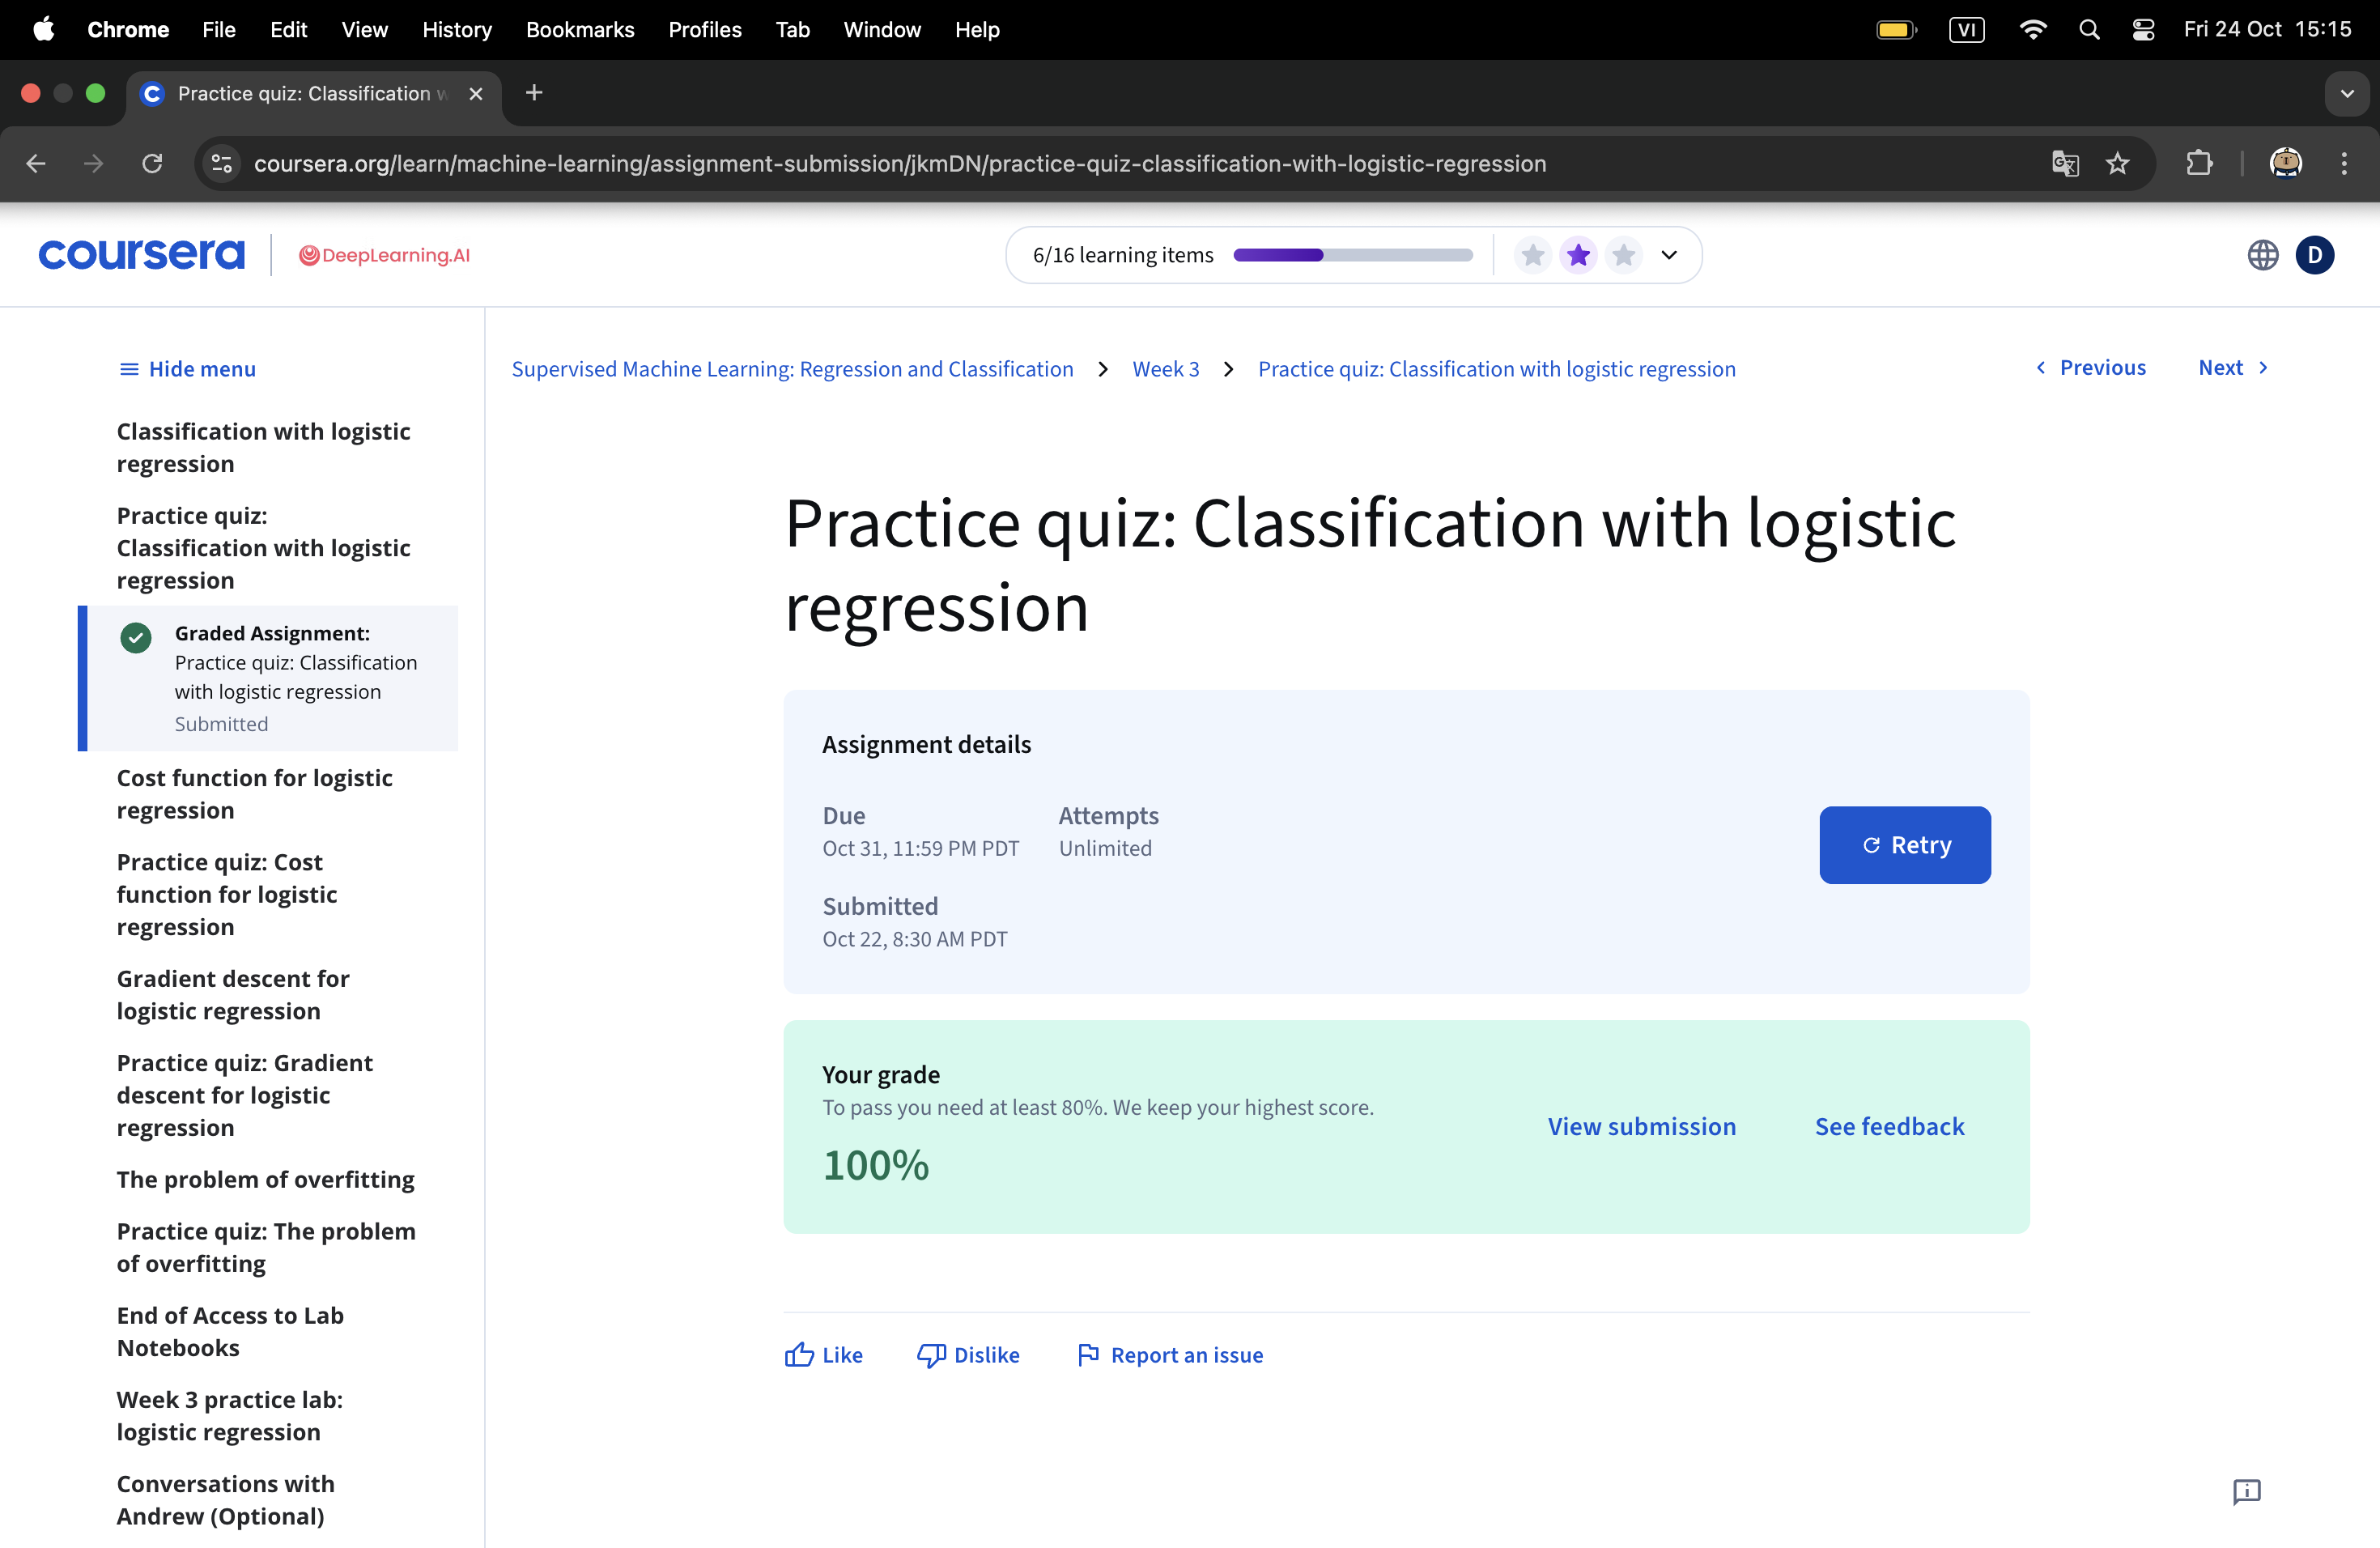
\includegraphics[scale=0.25]{Image/c1_w3_q1.png}
    \caption{Completed Graded Assignment 1 (Classification with logistic regression)}
\end{figure}

\begin{figure}[H]
    \centering
    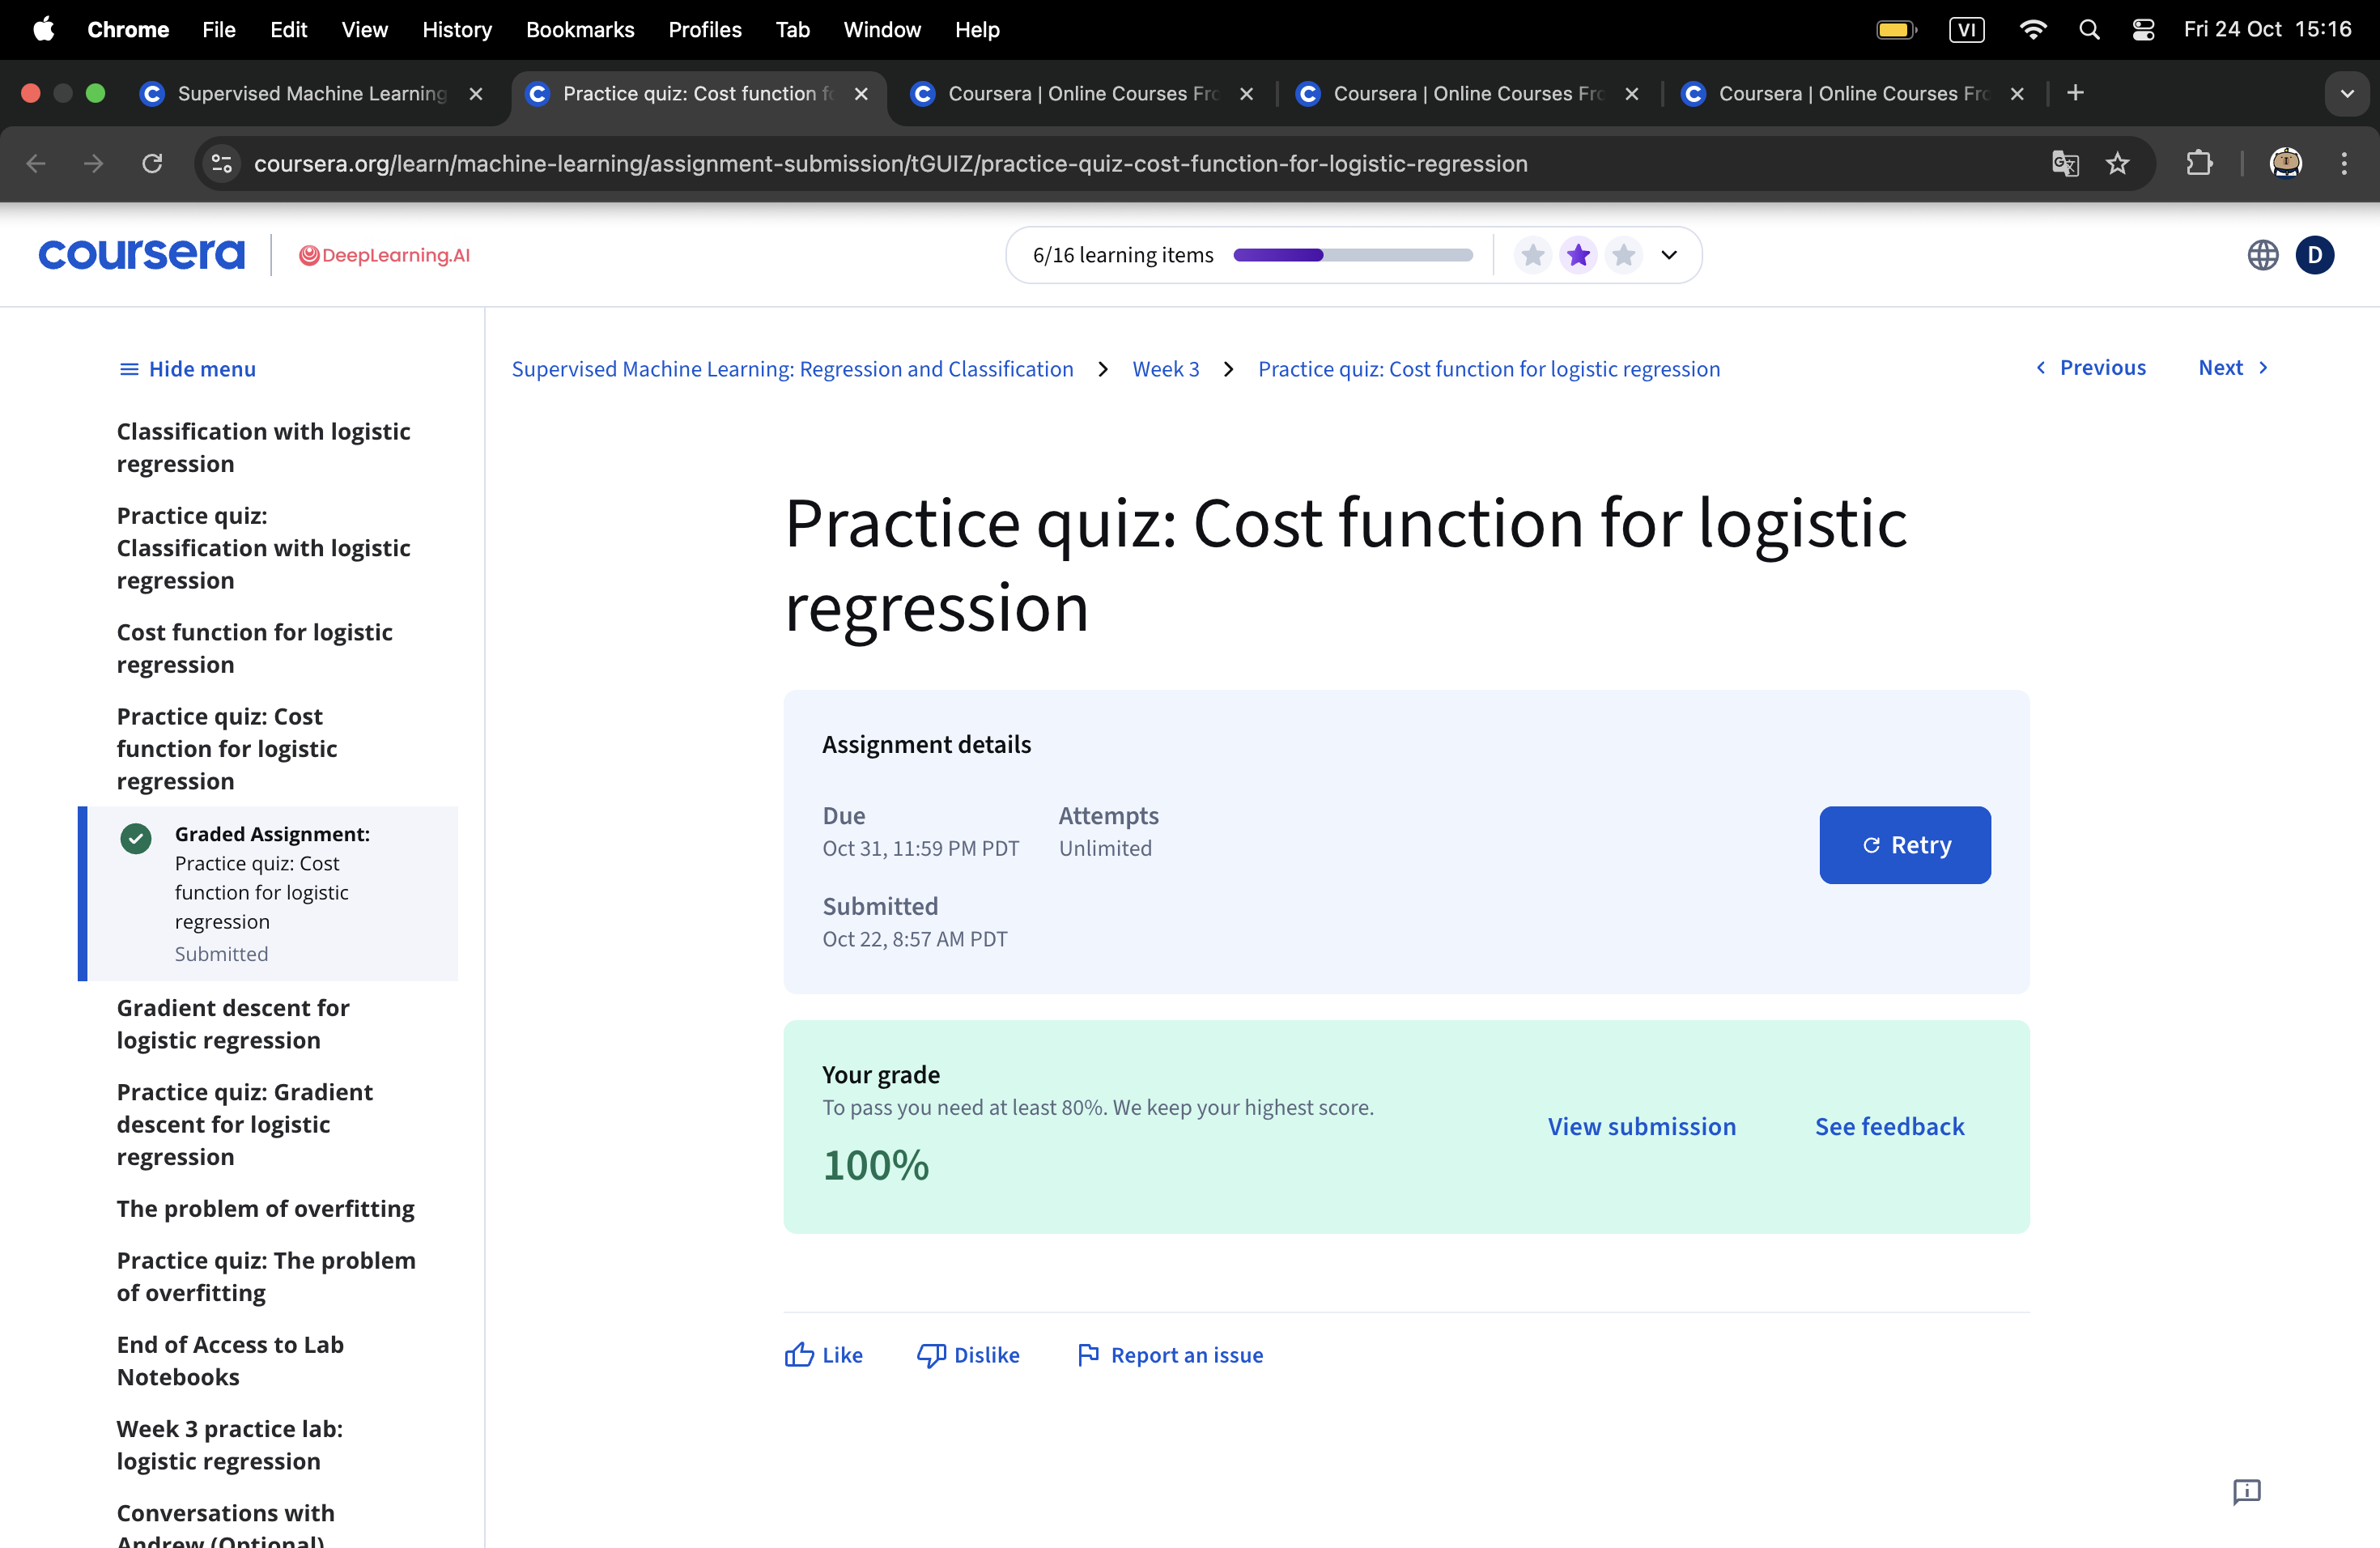
\includegraphics[scale=0.25]{Image/c1_w3_q2.png}
    \caption{Completed Graded Assignment 2 (Cost function for logistic regression)}
\end{figure}

\begin{figure}[H]
    \centering
    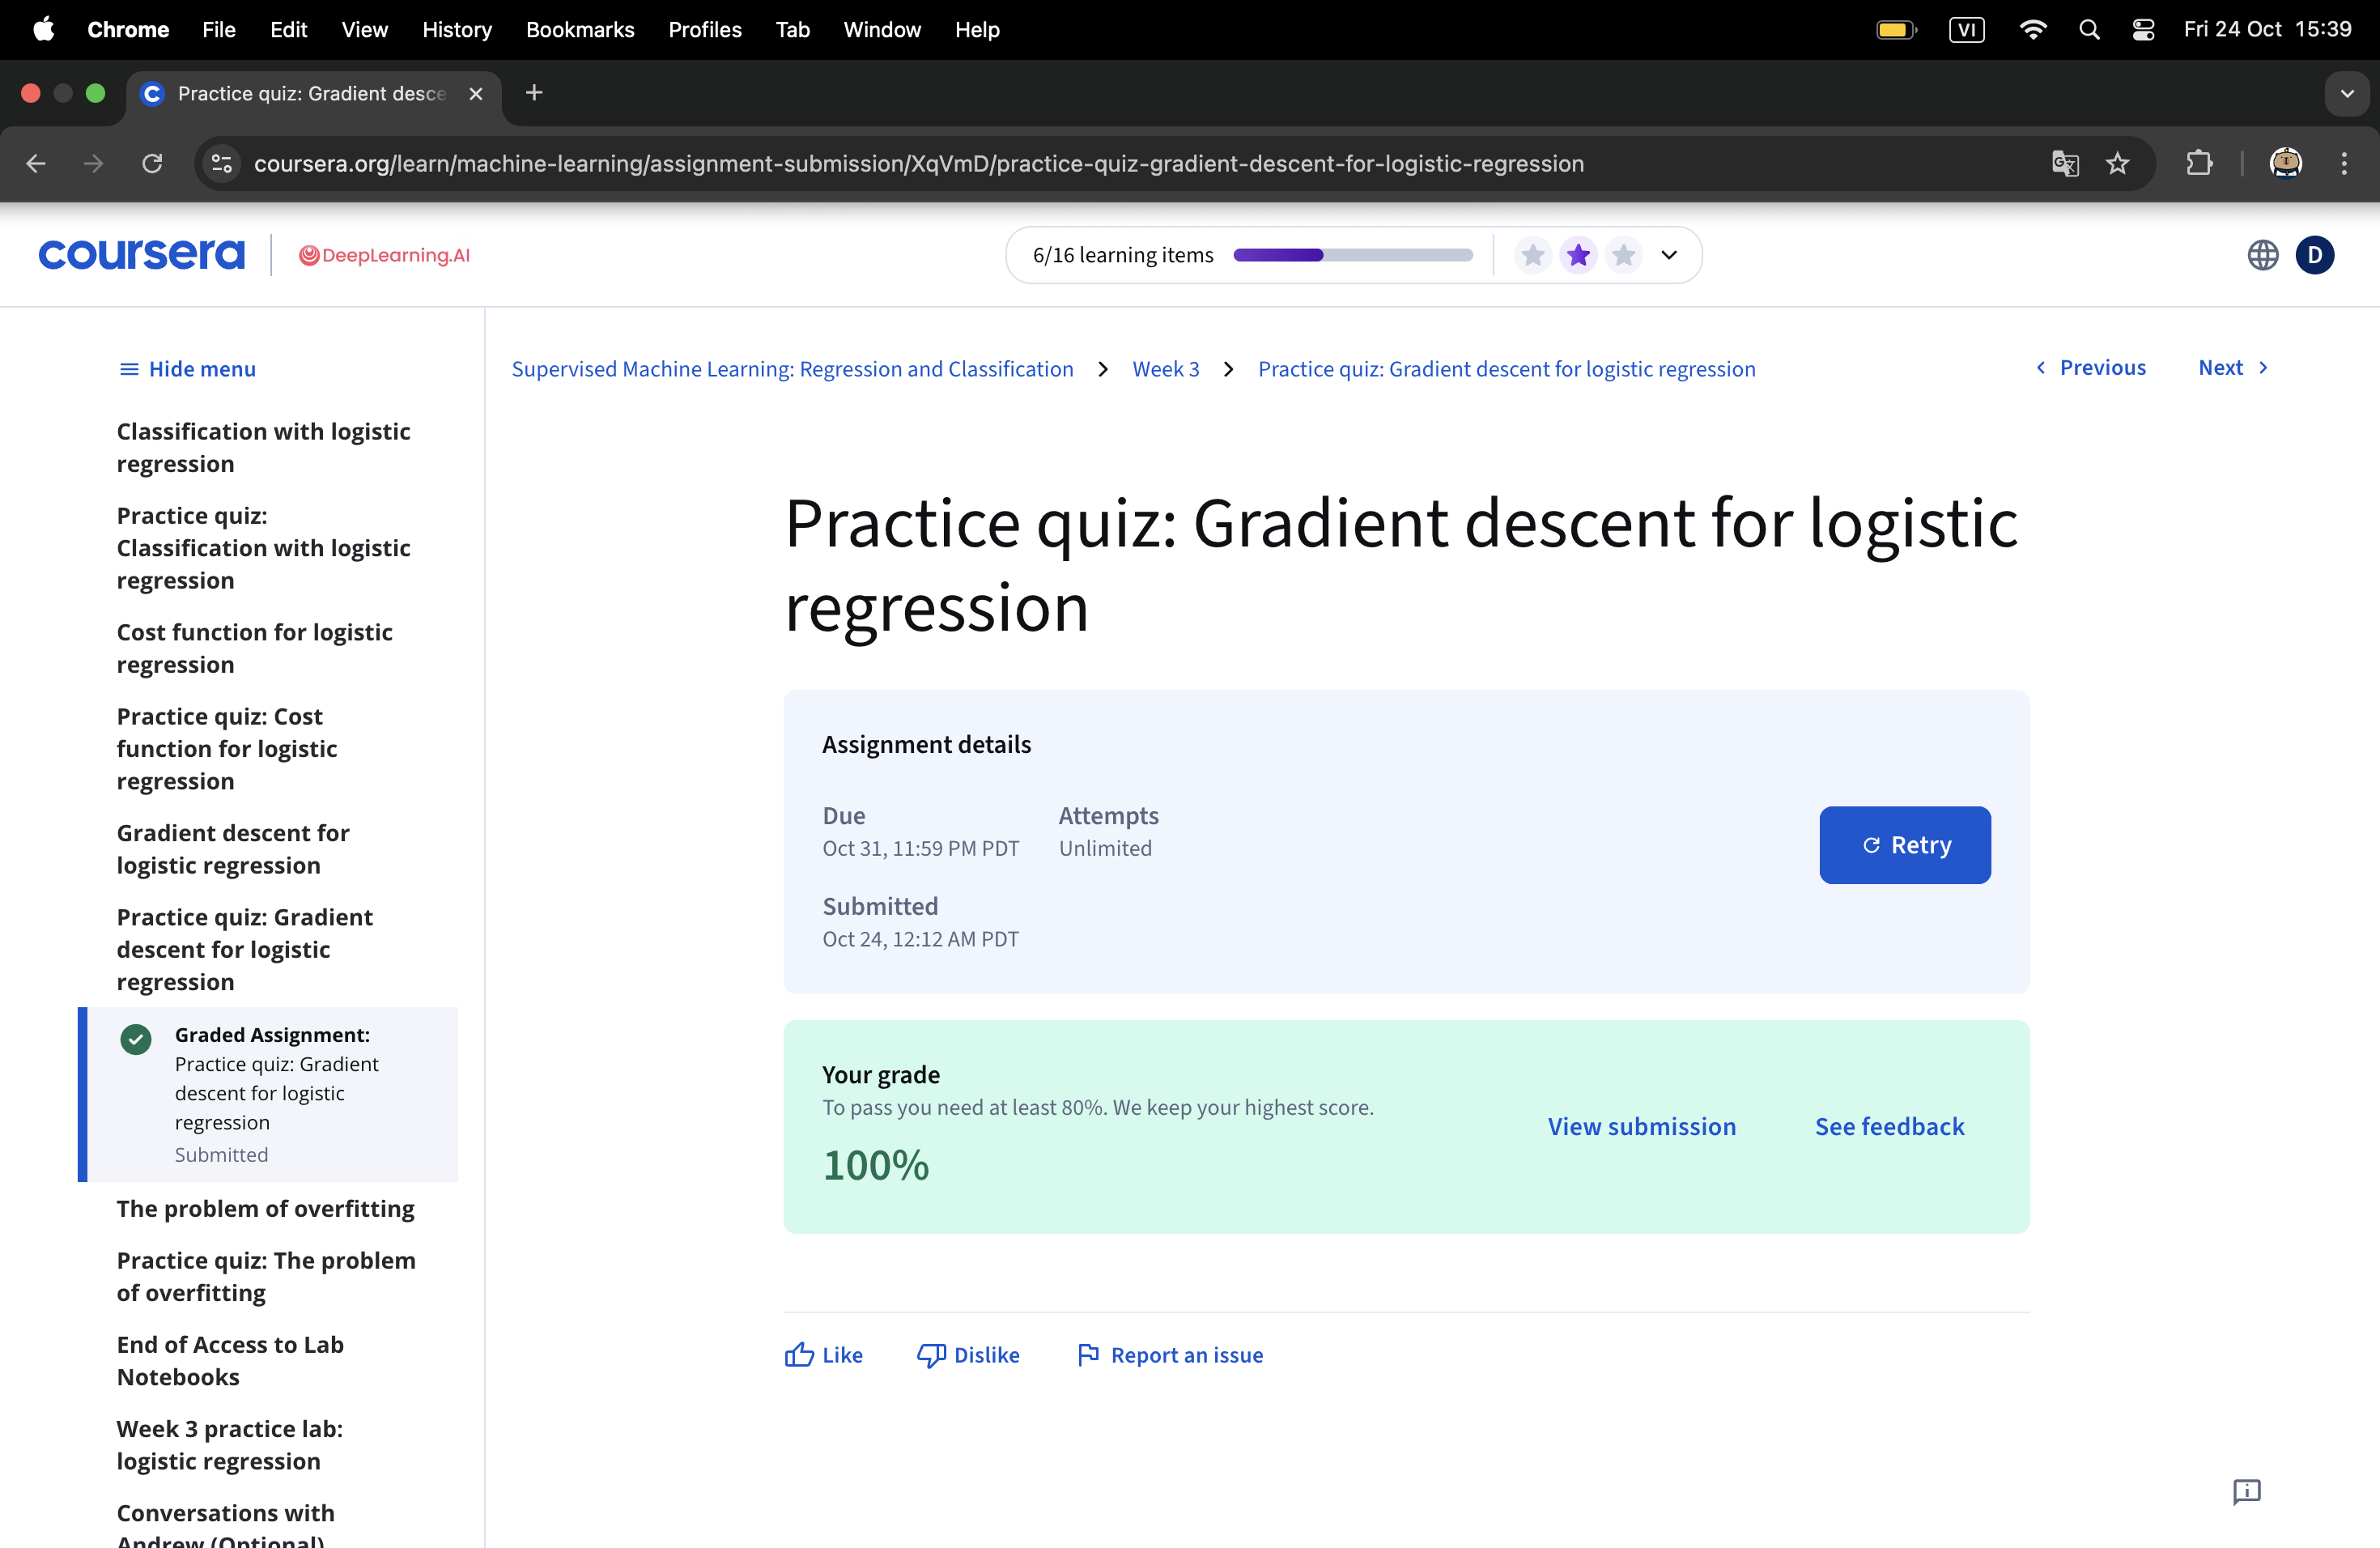
\includegraphics[scale=0.25]{Image/c1_w3_q3.png}
    \caption{Completed Graded Assignment 3 (Gradient descent for logistic regression)}
\end{figure}

\begin{figure}[H]
    \centering
    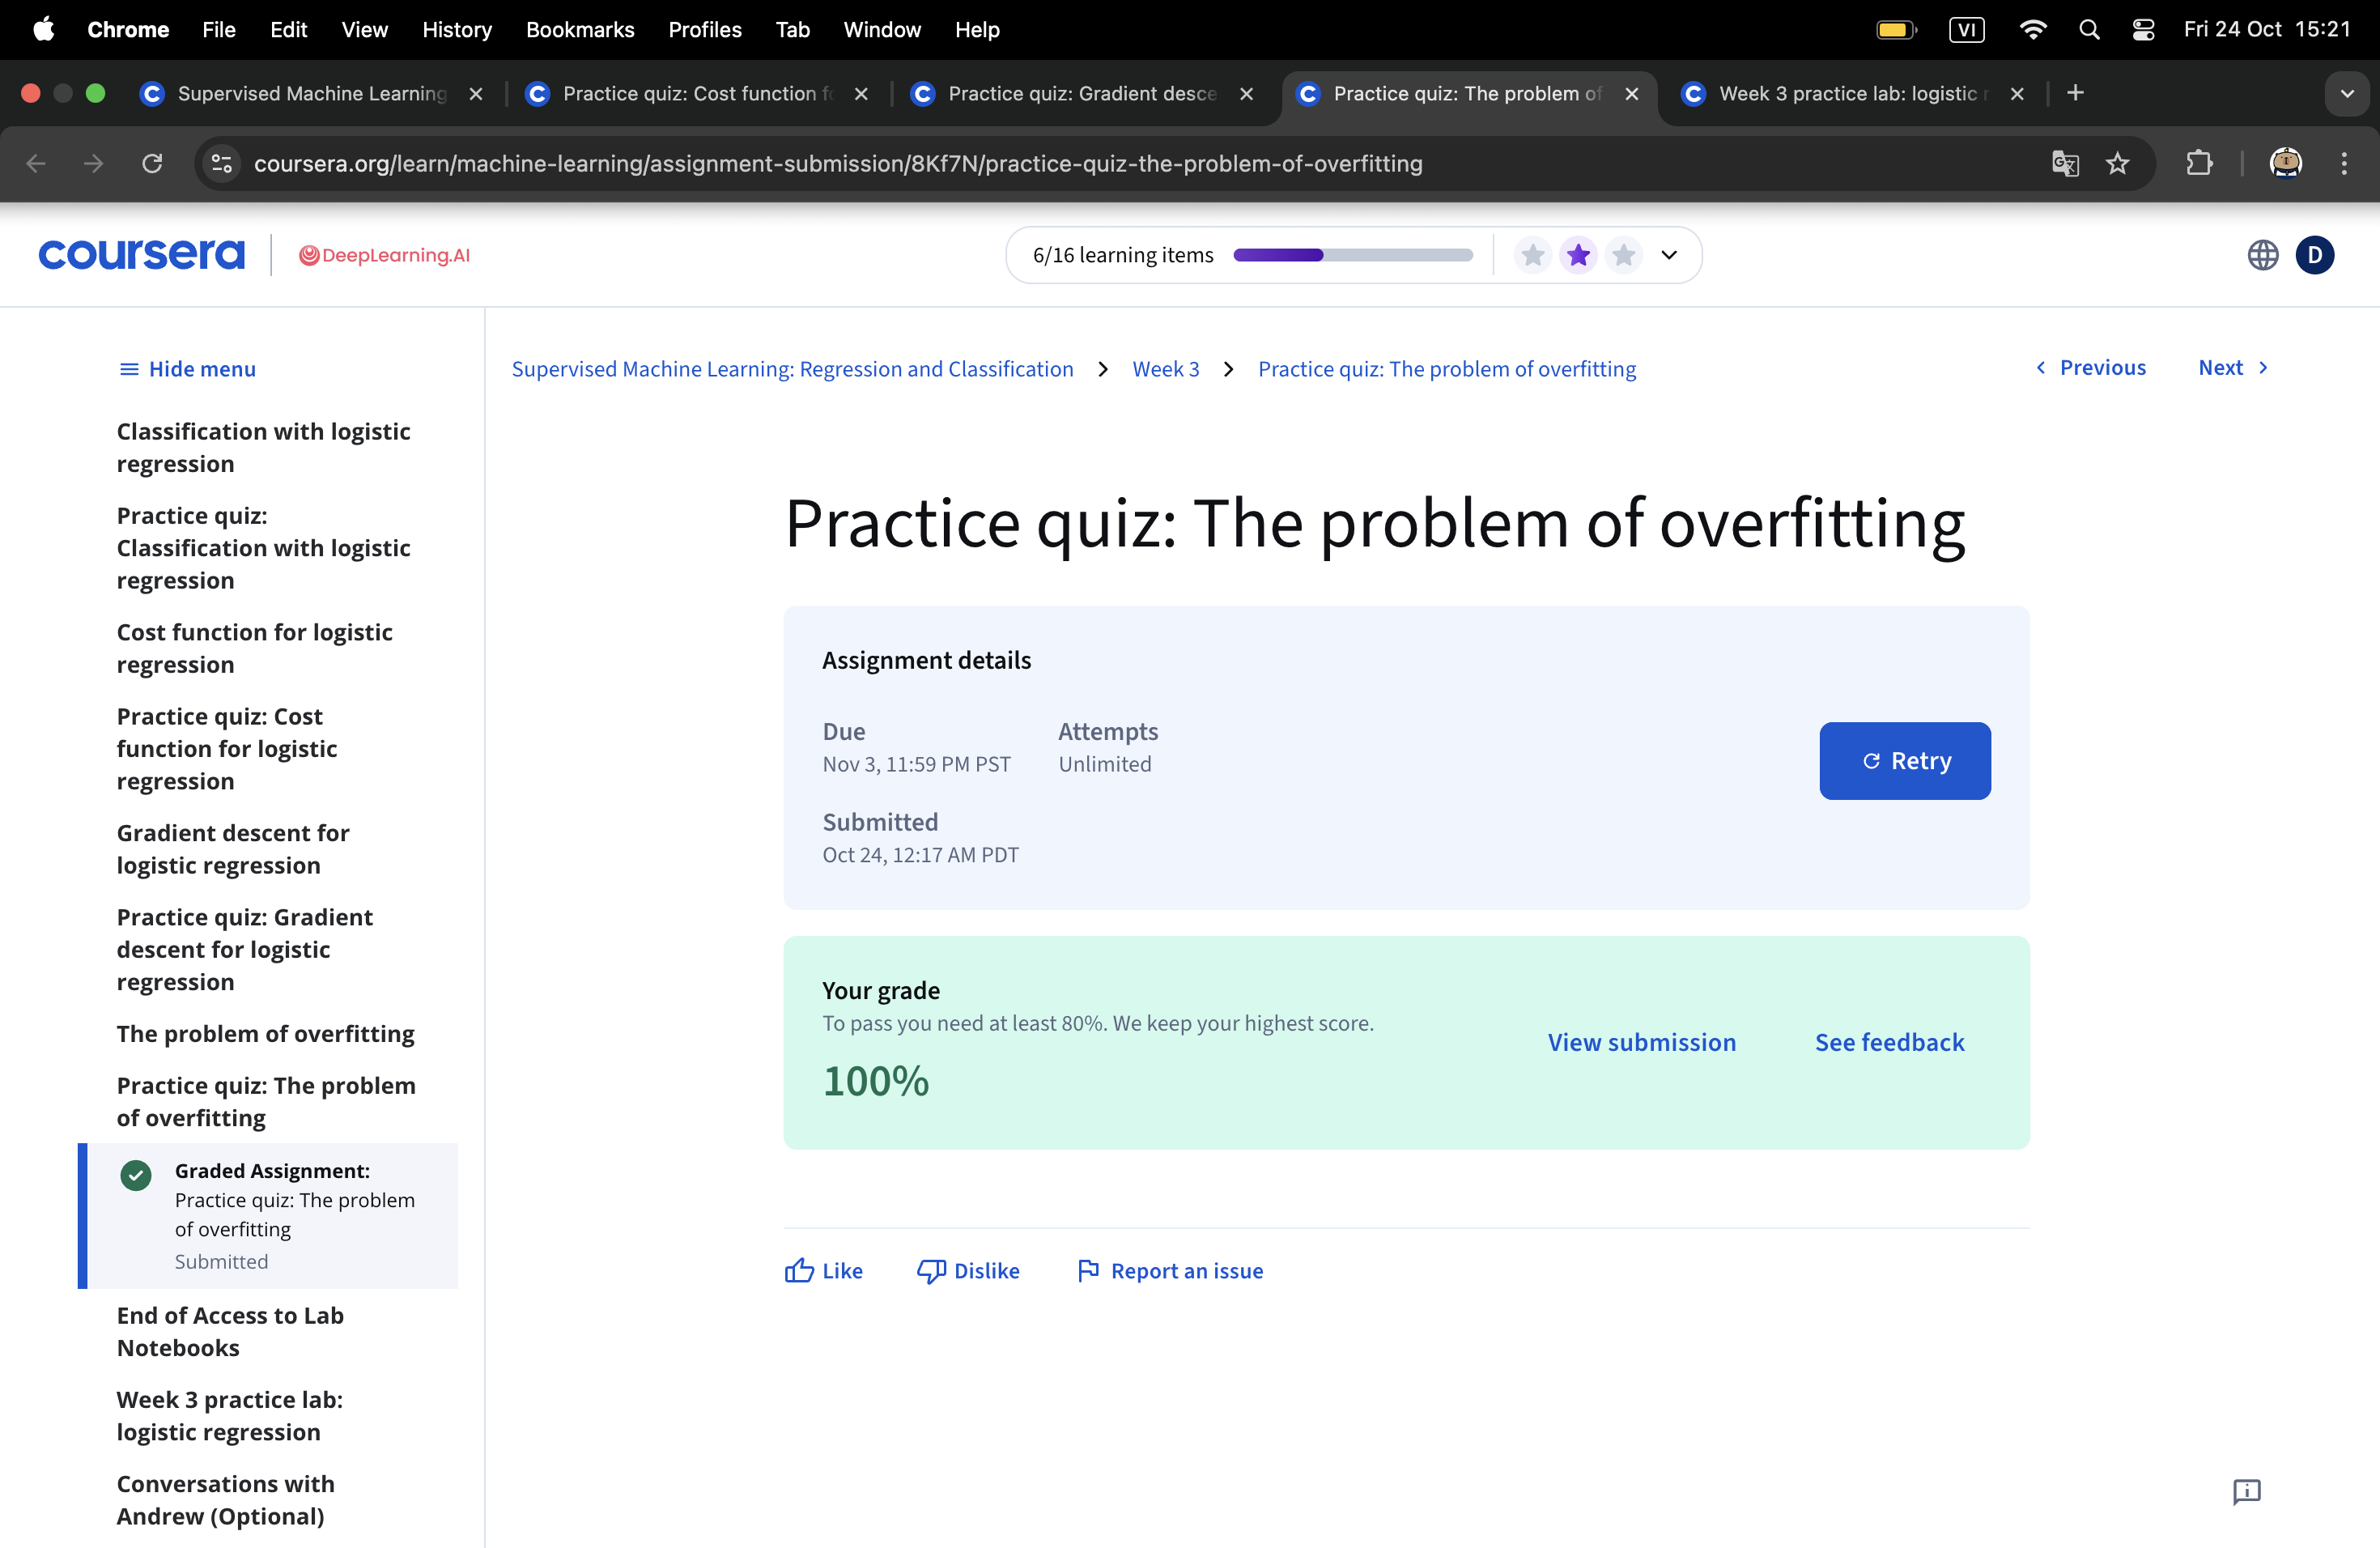
\includegraphics[scale=0.25]{Image/c1_w3_q4.png}
    \caption{Completed Graded Assignment 4 (The problem of overfitting)}
\end{figure}

\begin{figure}[H]
    \centering
    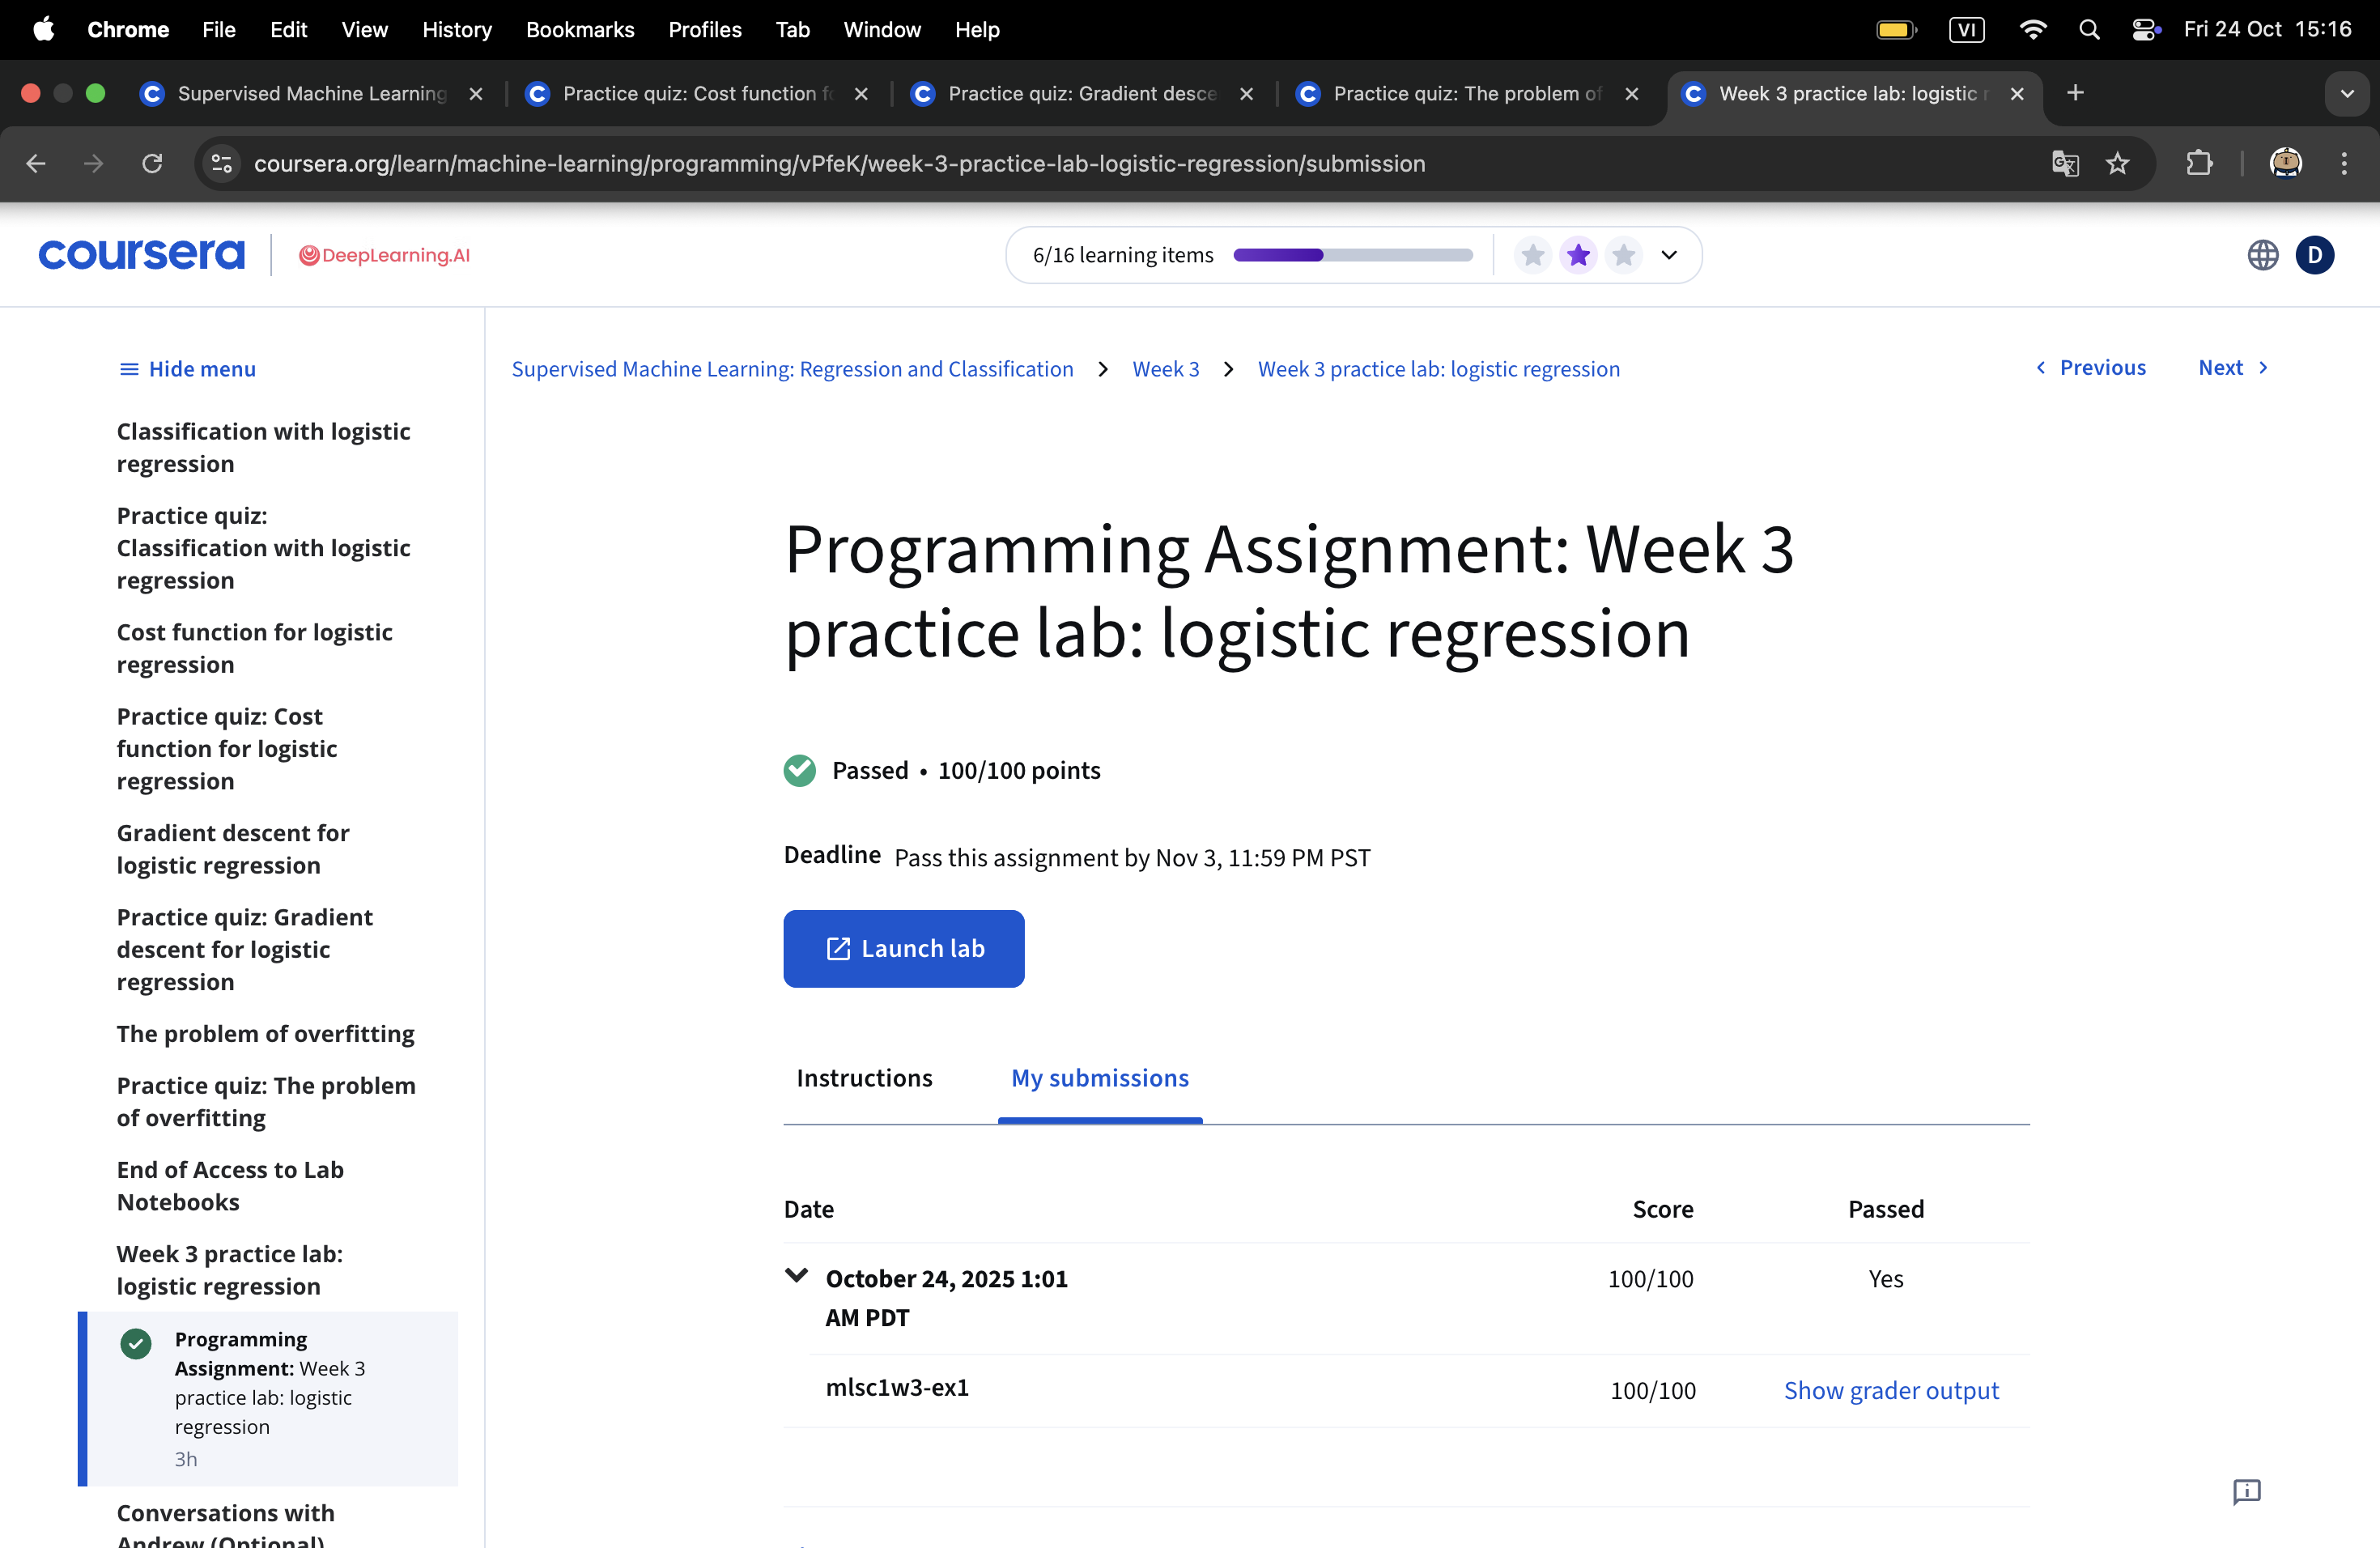
\includegraphics[scale=0.25]{Image/c1_w3_q5.png}
    \caption{Completed Programming Assignment (Logistic regression)}
\end{figure}

\subsection{Certificate for Completion}
\begin{figure}[H]
    \centering
    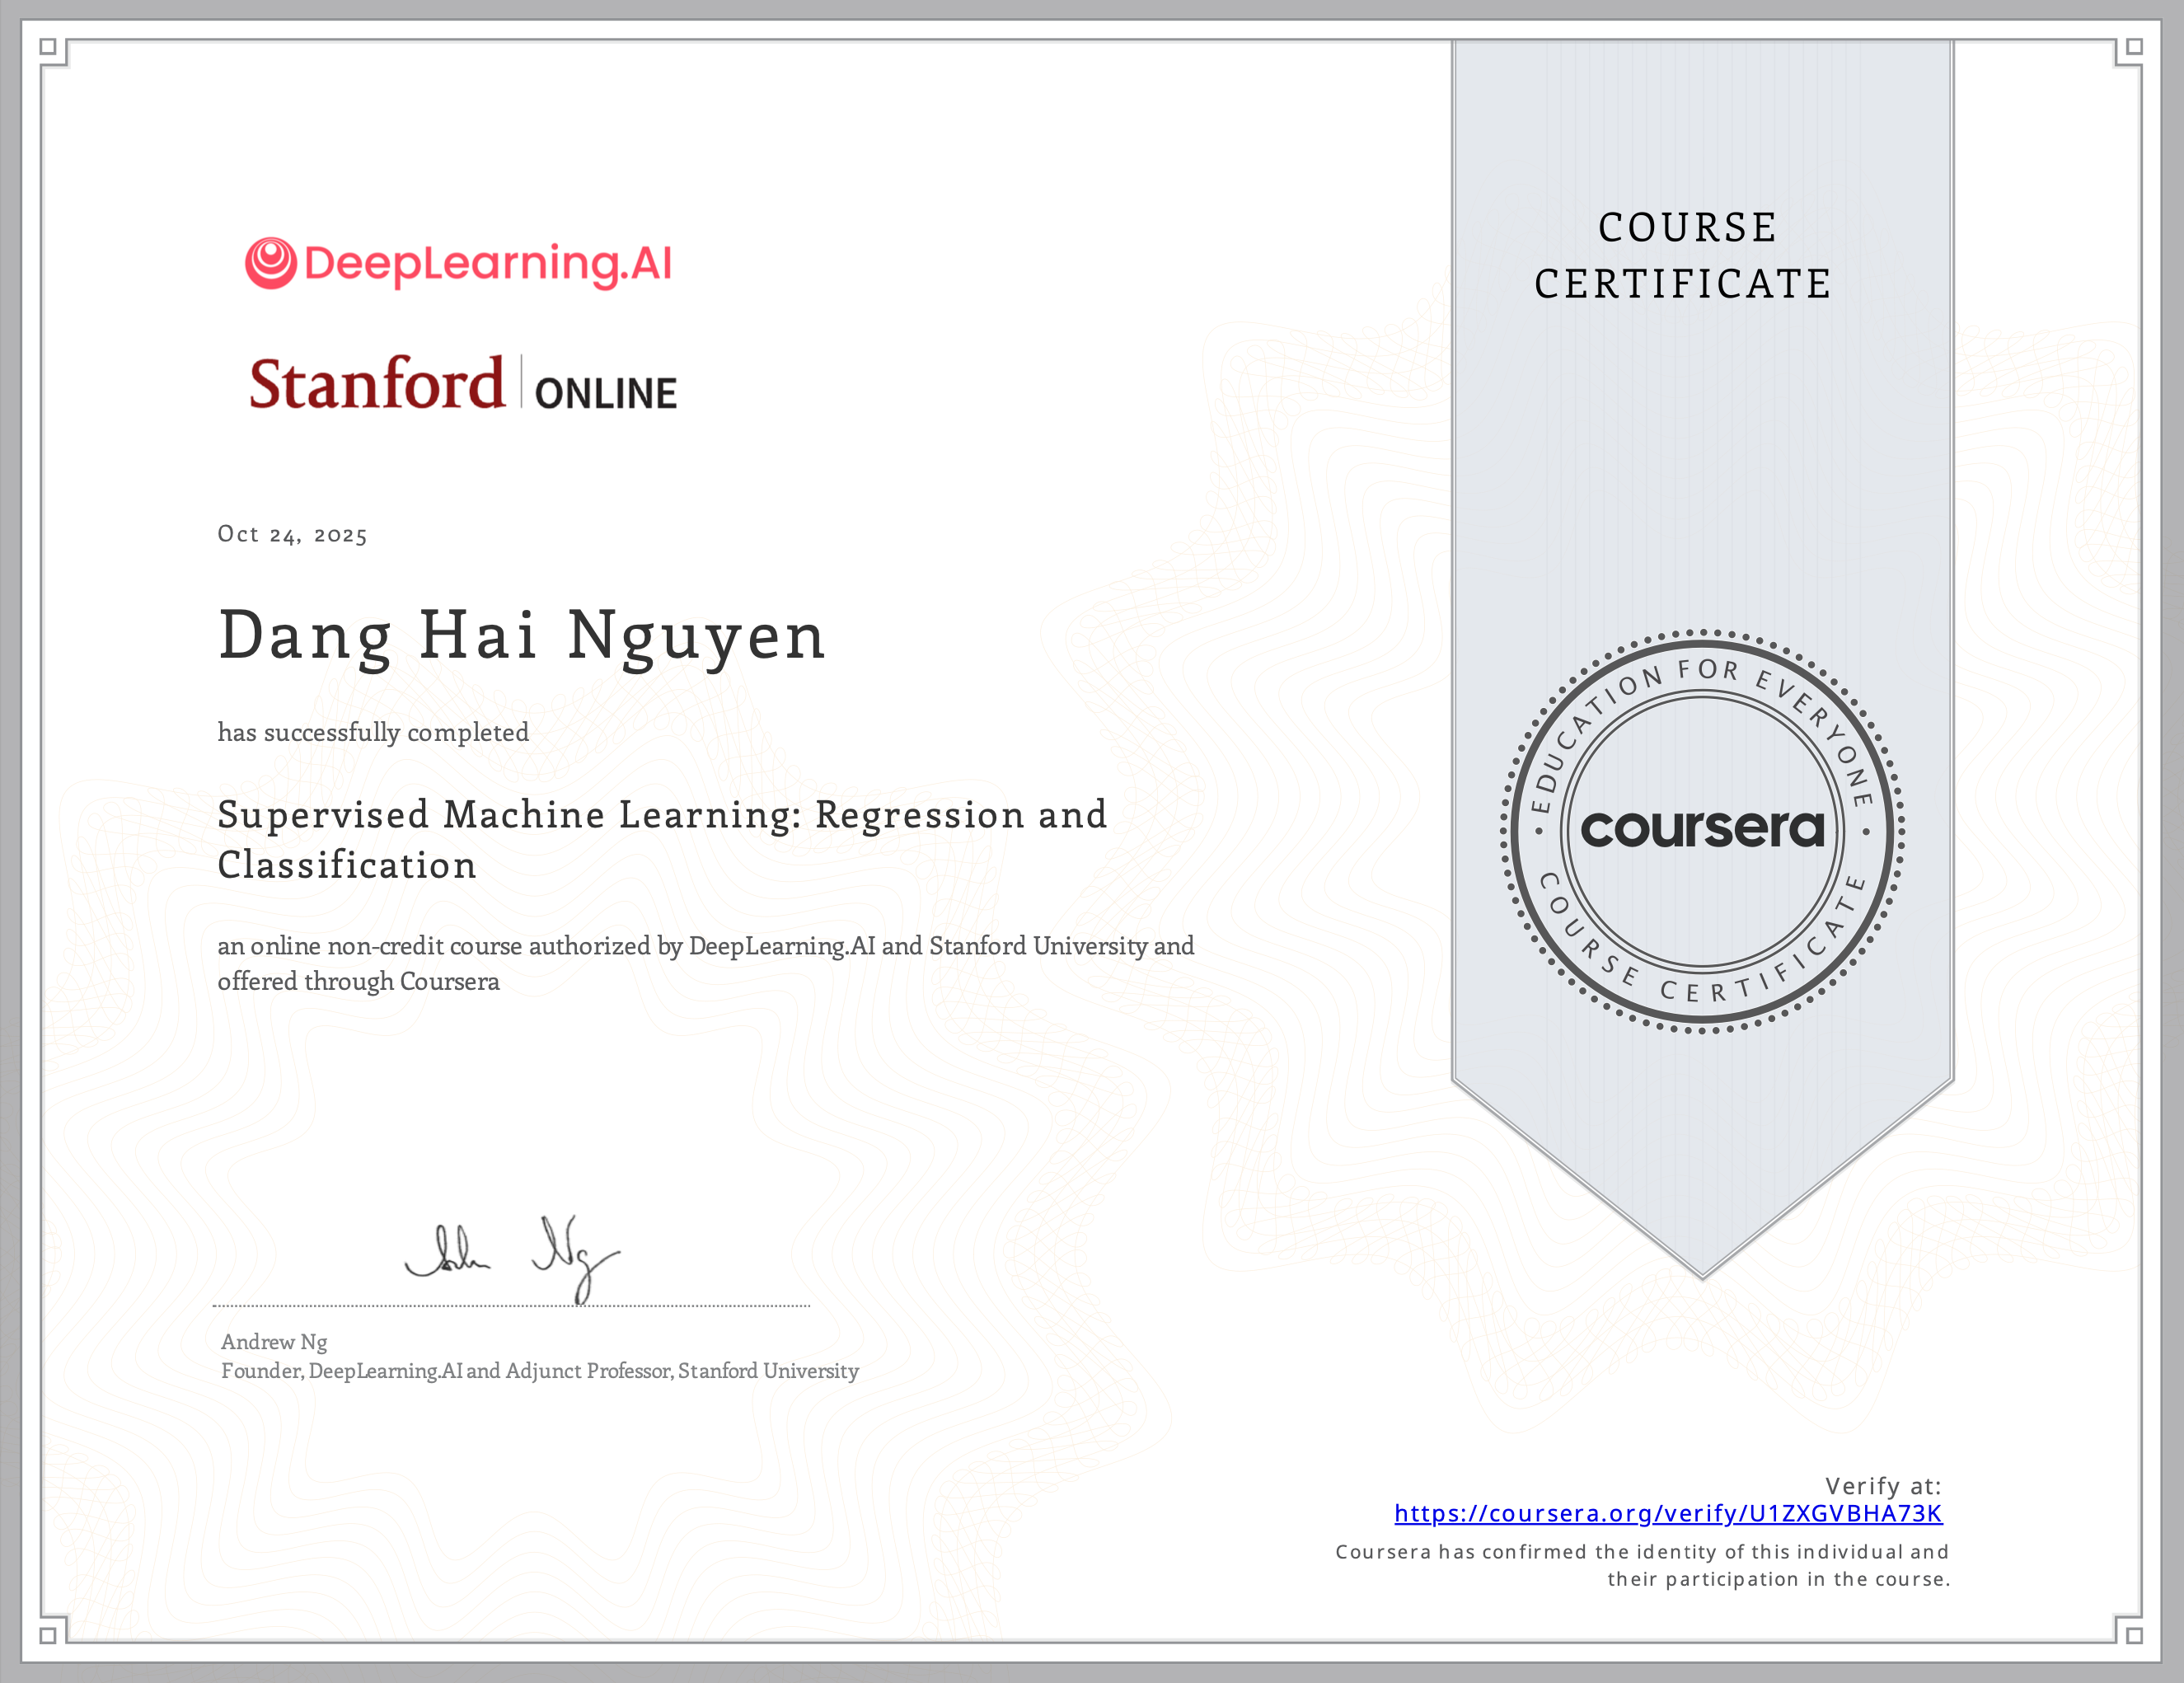
\includegraphics[scale=0.25]{Image/c1_certi.png}
    \caption{Certificate of completion for the course \textit{Supervised Machine Learning: Regression and Classification}.}
\end{figure}


%----------------------------------------
\section{Advanced Learning Algorithms}
%----------------------------------------

Building upon the foundational regression and classification models, this course delves into high-capacity models capable of capturing complex, non-linear patterns. It moves from the theoretical underpinnings of Neural Networks to the practical methodology of building, diagnosing, and optimizing real-world machine learning systems.

\begin{figure}[H]
    \centering
    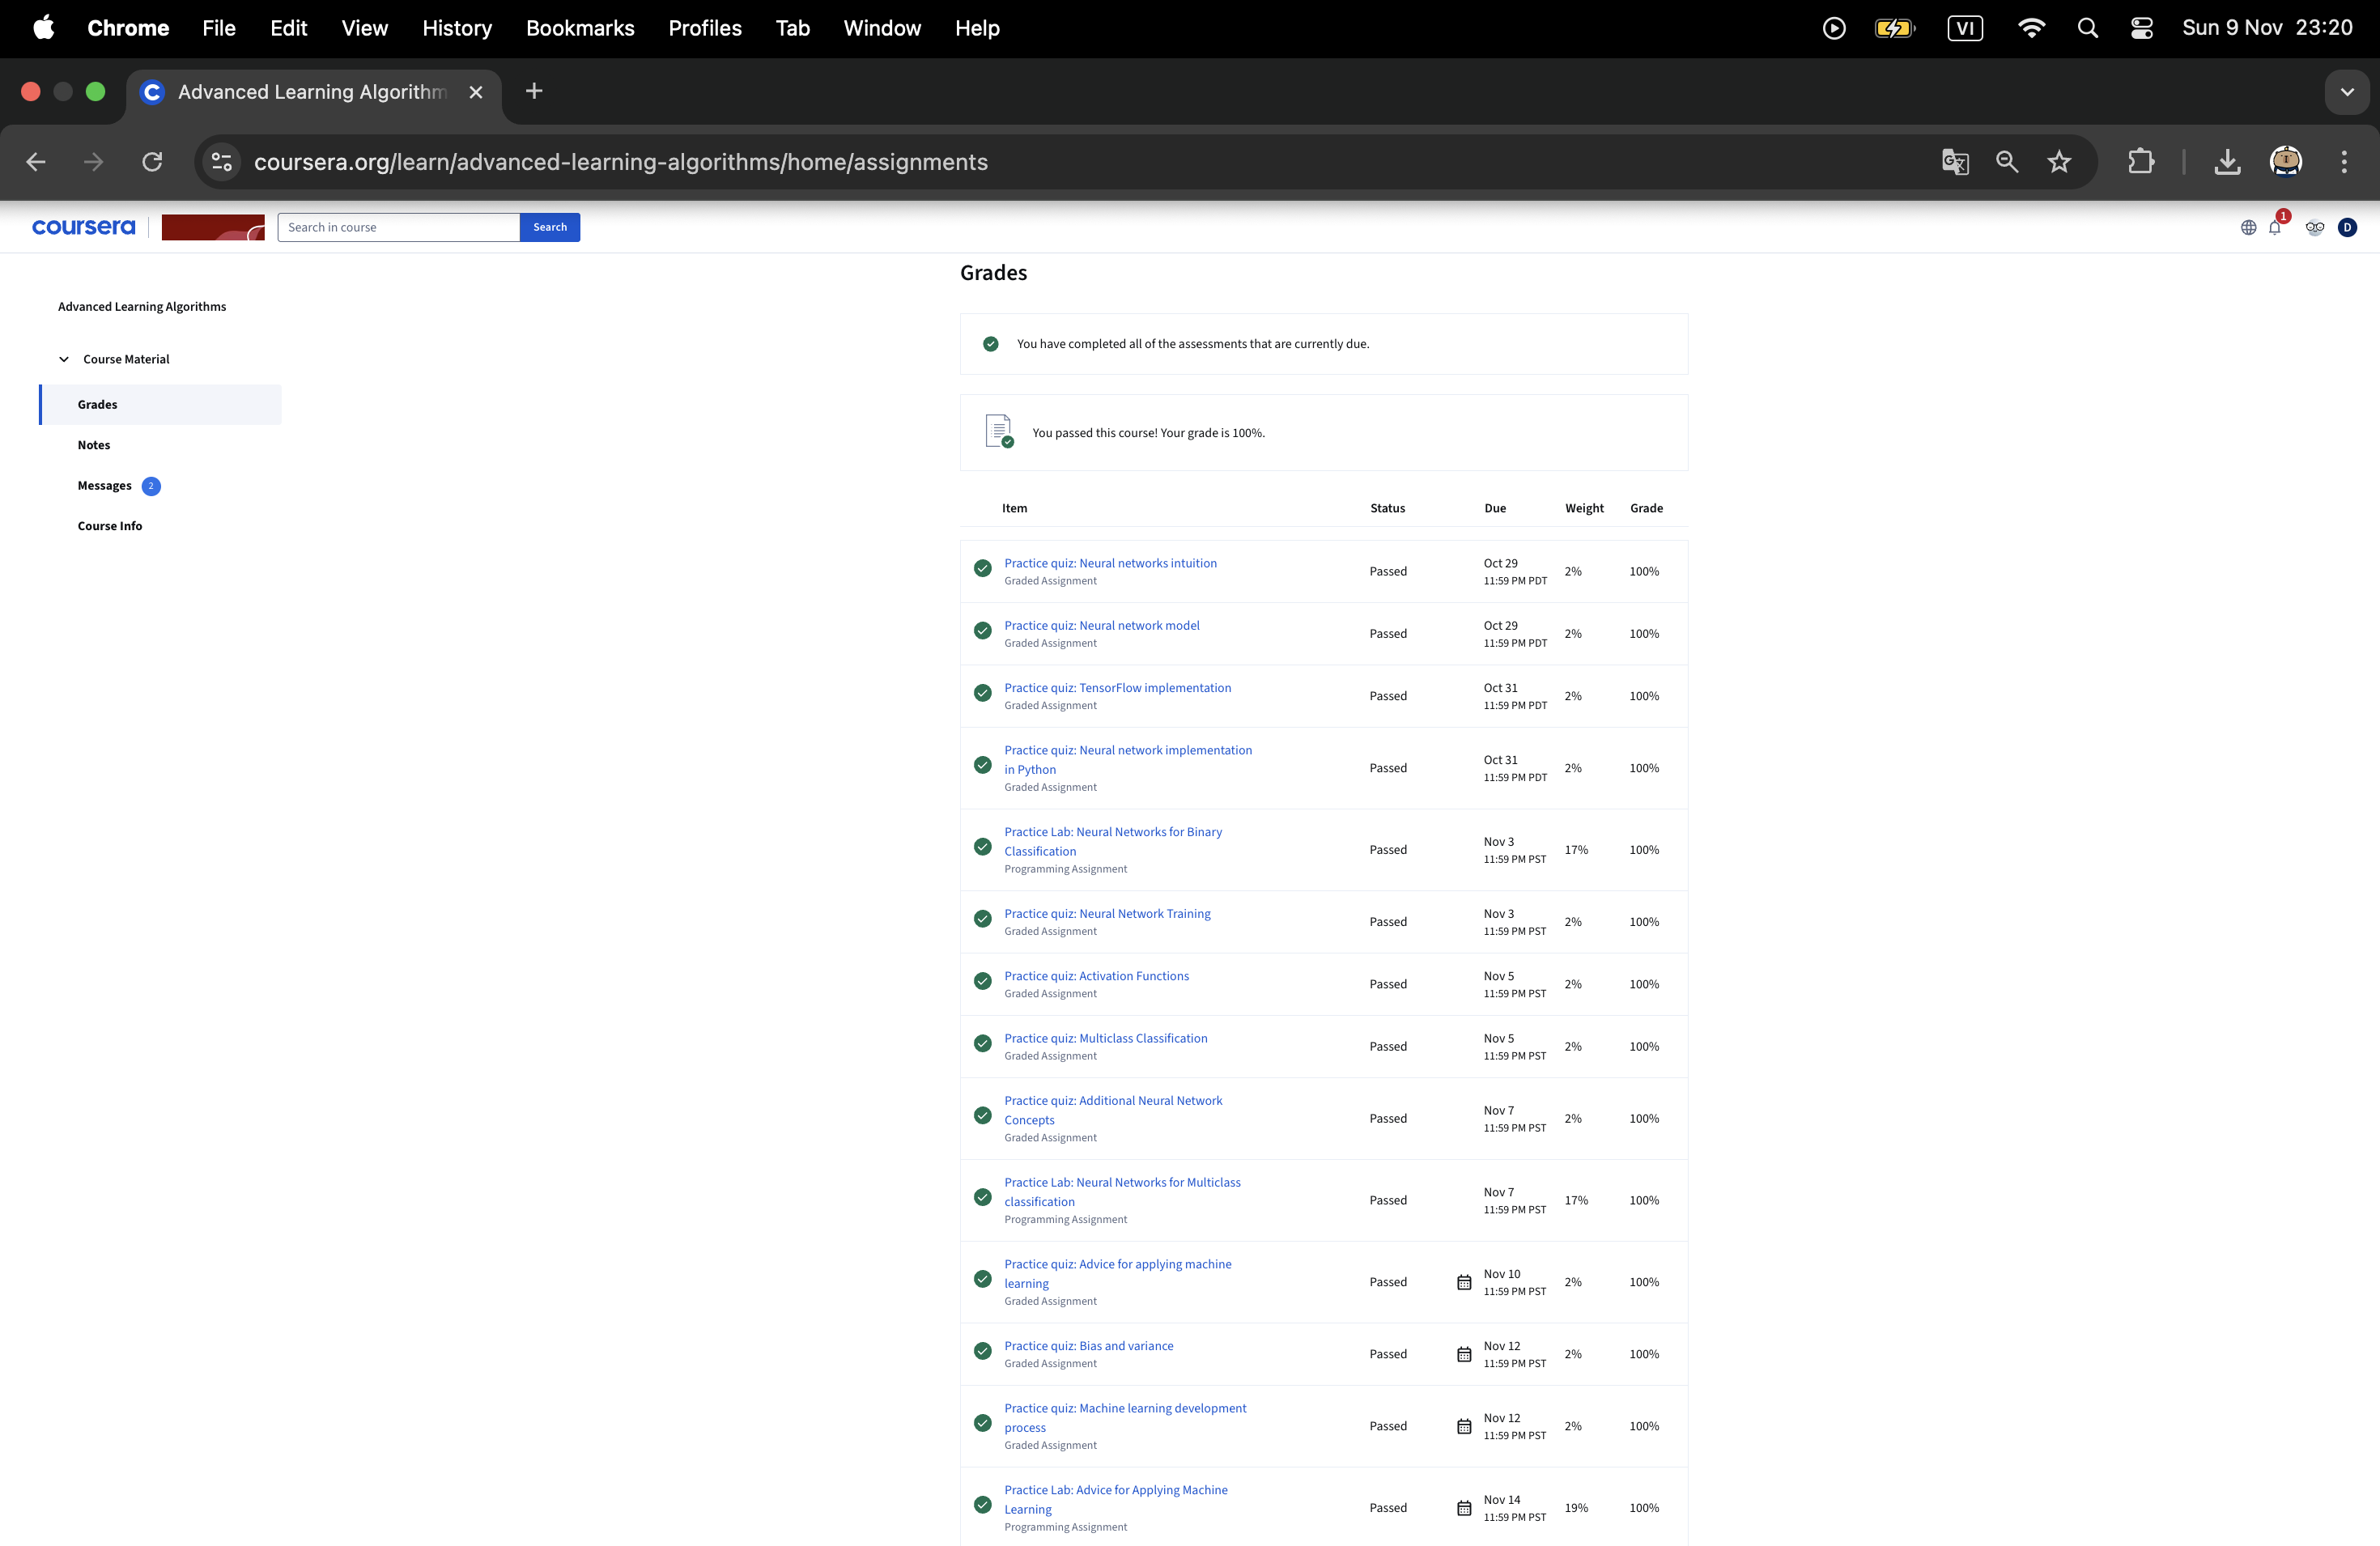
\includegraphics[scale=0.3]{Image/c2.png}
    \caption{Course 2 completed}
\end{figure}

%----------------------------------------
\subsection{Week 1: Neural Networks}
%----------------------------------------

\subsubsection{Key Insights and Learnings}

This module marked the transition from traditional algorithms to Deep Learning, utilizing biological inspiration to solve complex computational problems.

\begin{itemize}
    \item \textbf{Neural Network Architecture:} Understood how stacking layers of logistic regression units creates a "Multi-Layer Perceptron."
    \begin{itemize}
        \item \textbf{Activation Functions:} Analyzed the role of non-linear functions like \textbf{ReLU} (Rectified Linear Unit) for hidden layers to avoid the "vanishing gradient" problem and \textbf{Sigmoid} for binary output.
        \item \textbf{Vectorization:} Leveraged matrix multiplication (via TensorFlow/NumPy) to perform forward propagation efficiently over large datasets.
    \end{itemize}

    \item \textbf{Multiclass Classification (Softmax):} Extended binary classification to multiple categories using the \textbf{Softmax Regression} function, which outputs a probability distribution across $N$ classes (ensuring $\sum P(y=k) = 1$).
    
    \item \textbf{Hierarchical Feature Learning:} Recognized that deep networks learn representations hierarchically—lower layers detect simple edges, while deeper layers assemble them into complex shapes and objects.
\end{itemize}

\subsubsection{Learning Evidence}
\begin{figure}[H]
    \centering
    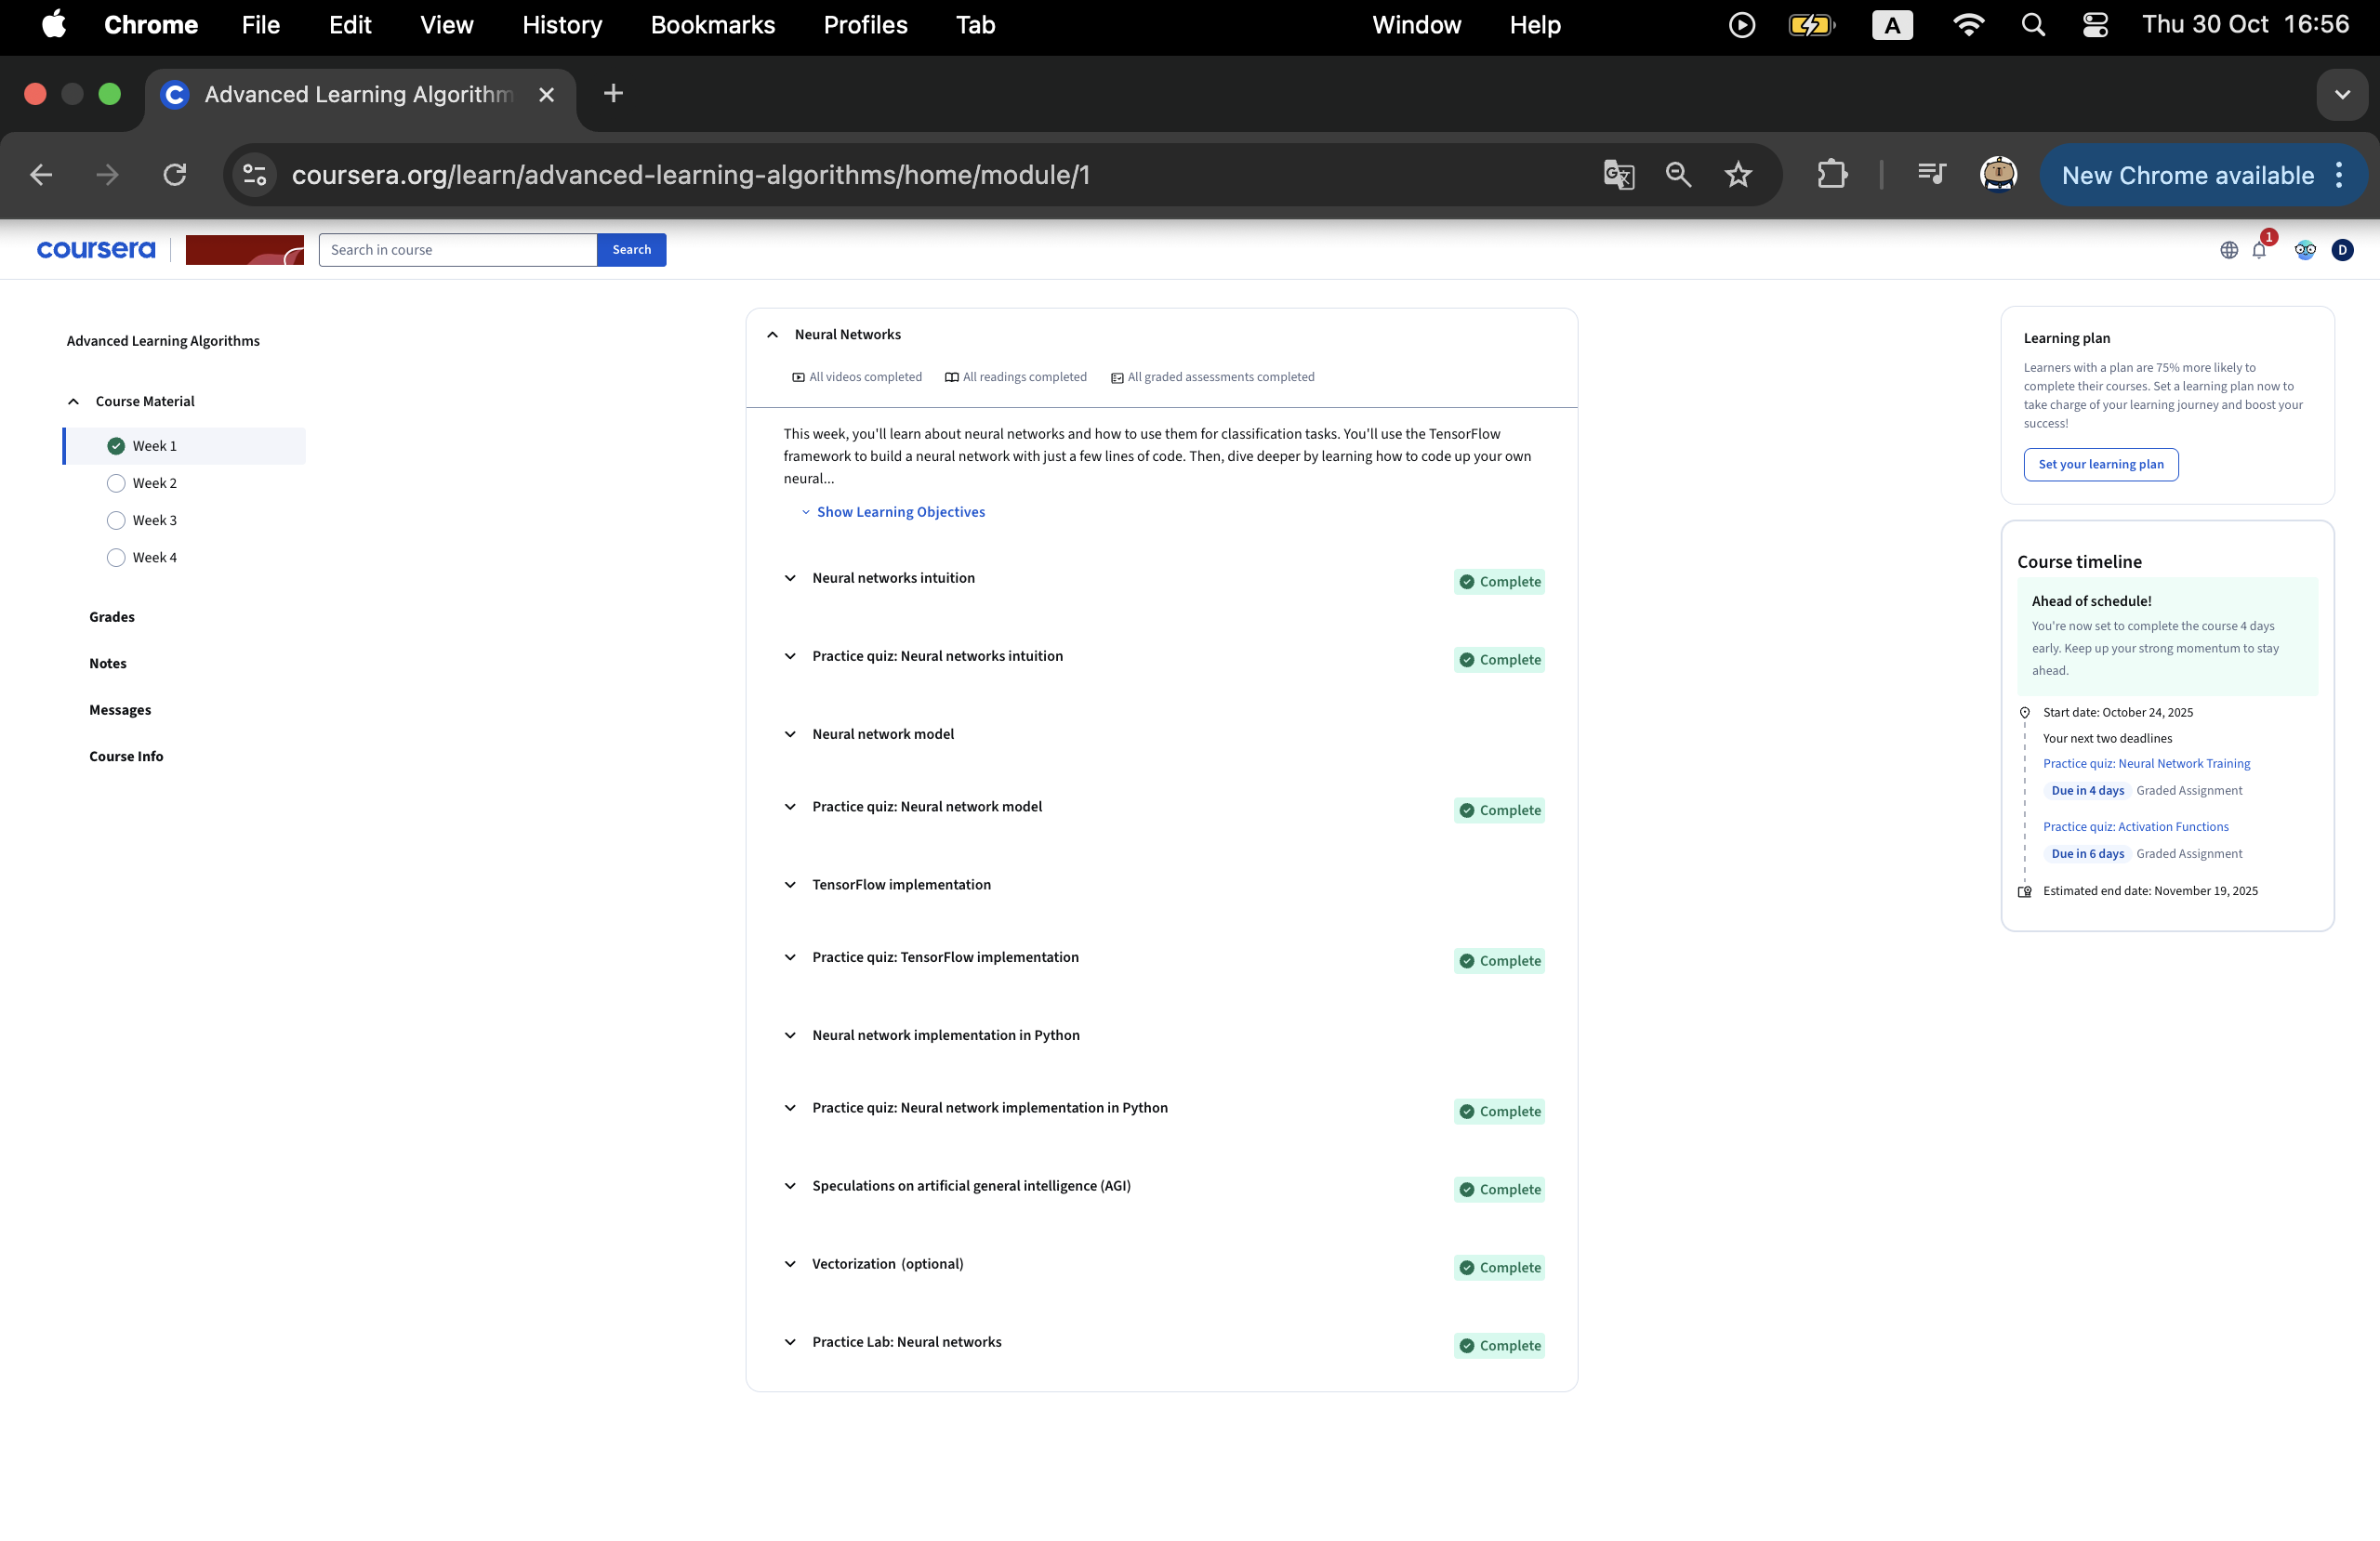
\includegraphics[scale=0.25]{Image/c2_w1.png}
    \caption{Lesson's completed date (30/10/2025)}
\end{figure}

\subsubsection{Graded Assignment Evidence}
\begin{figure}[H]
    \centering
    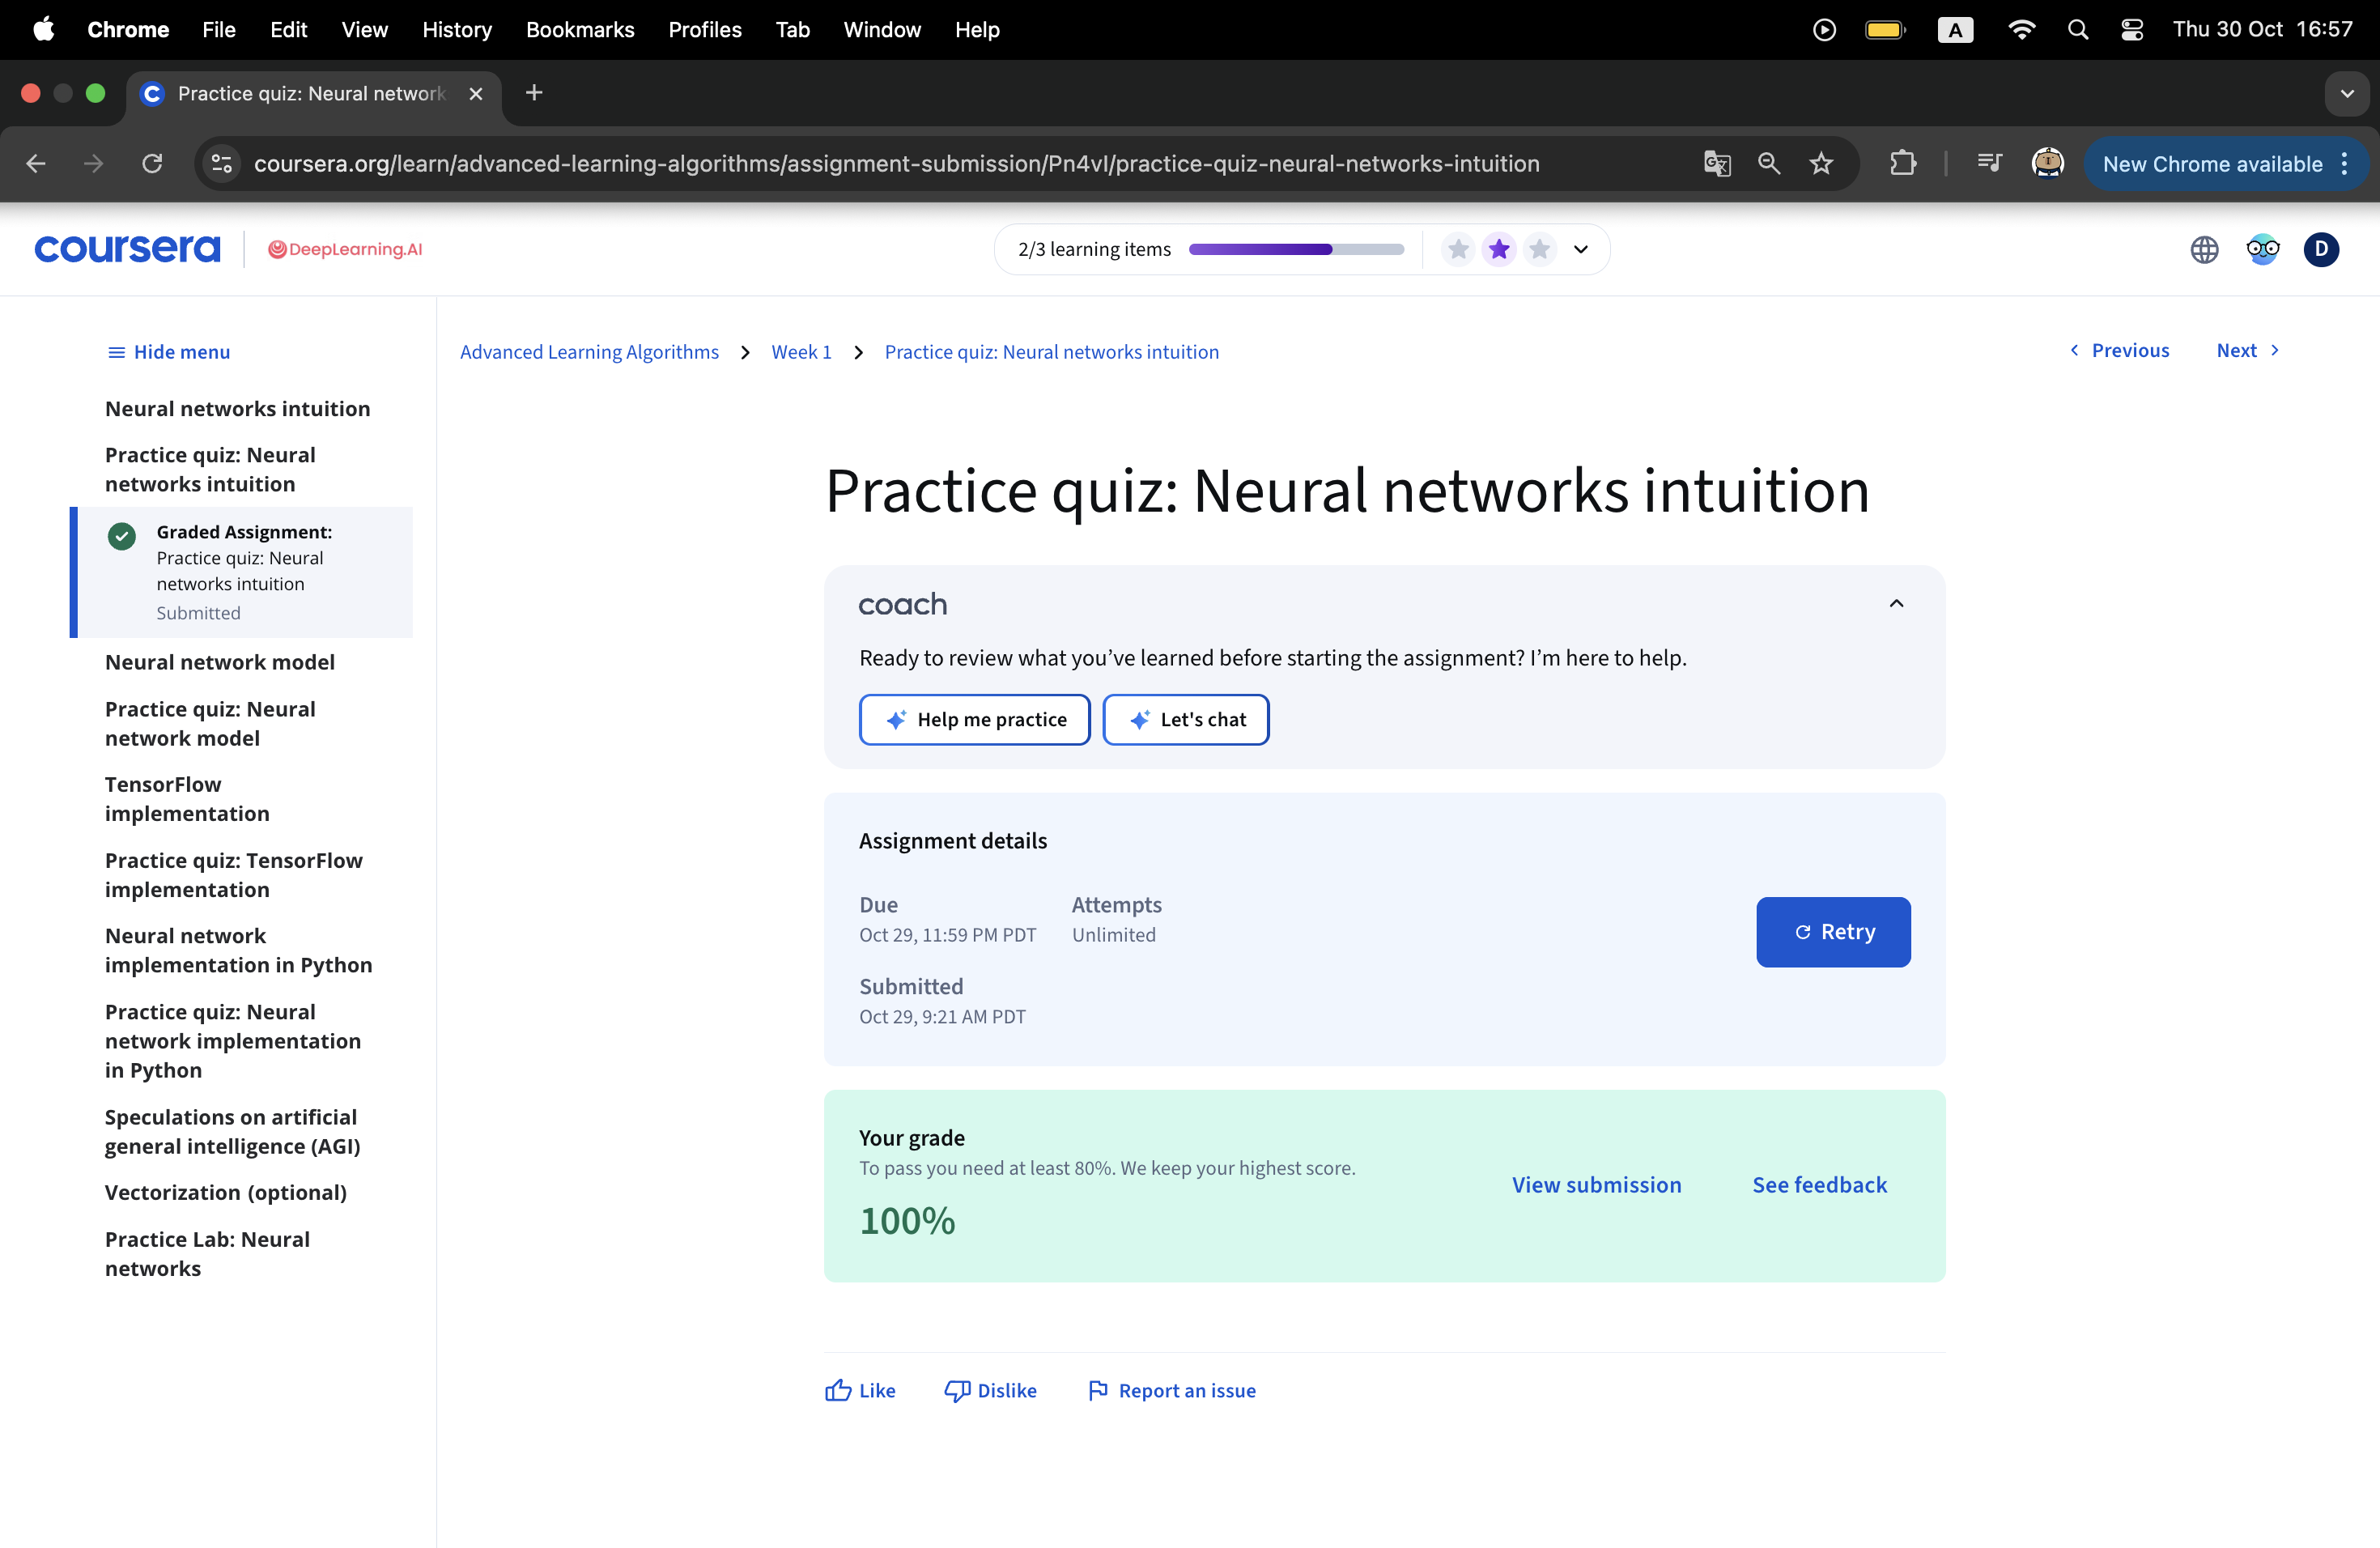
\includegraphics[scale=0.27]{Image/c2_w1_q1.png}
    \caption{Completed Graded Assignment 1 (Neural networks intuition)}
\end{figure}

\begin{figure}[H]
    \centering
    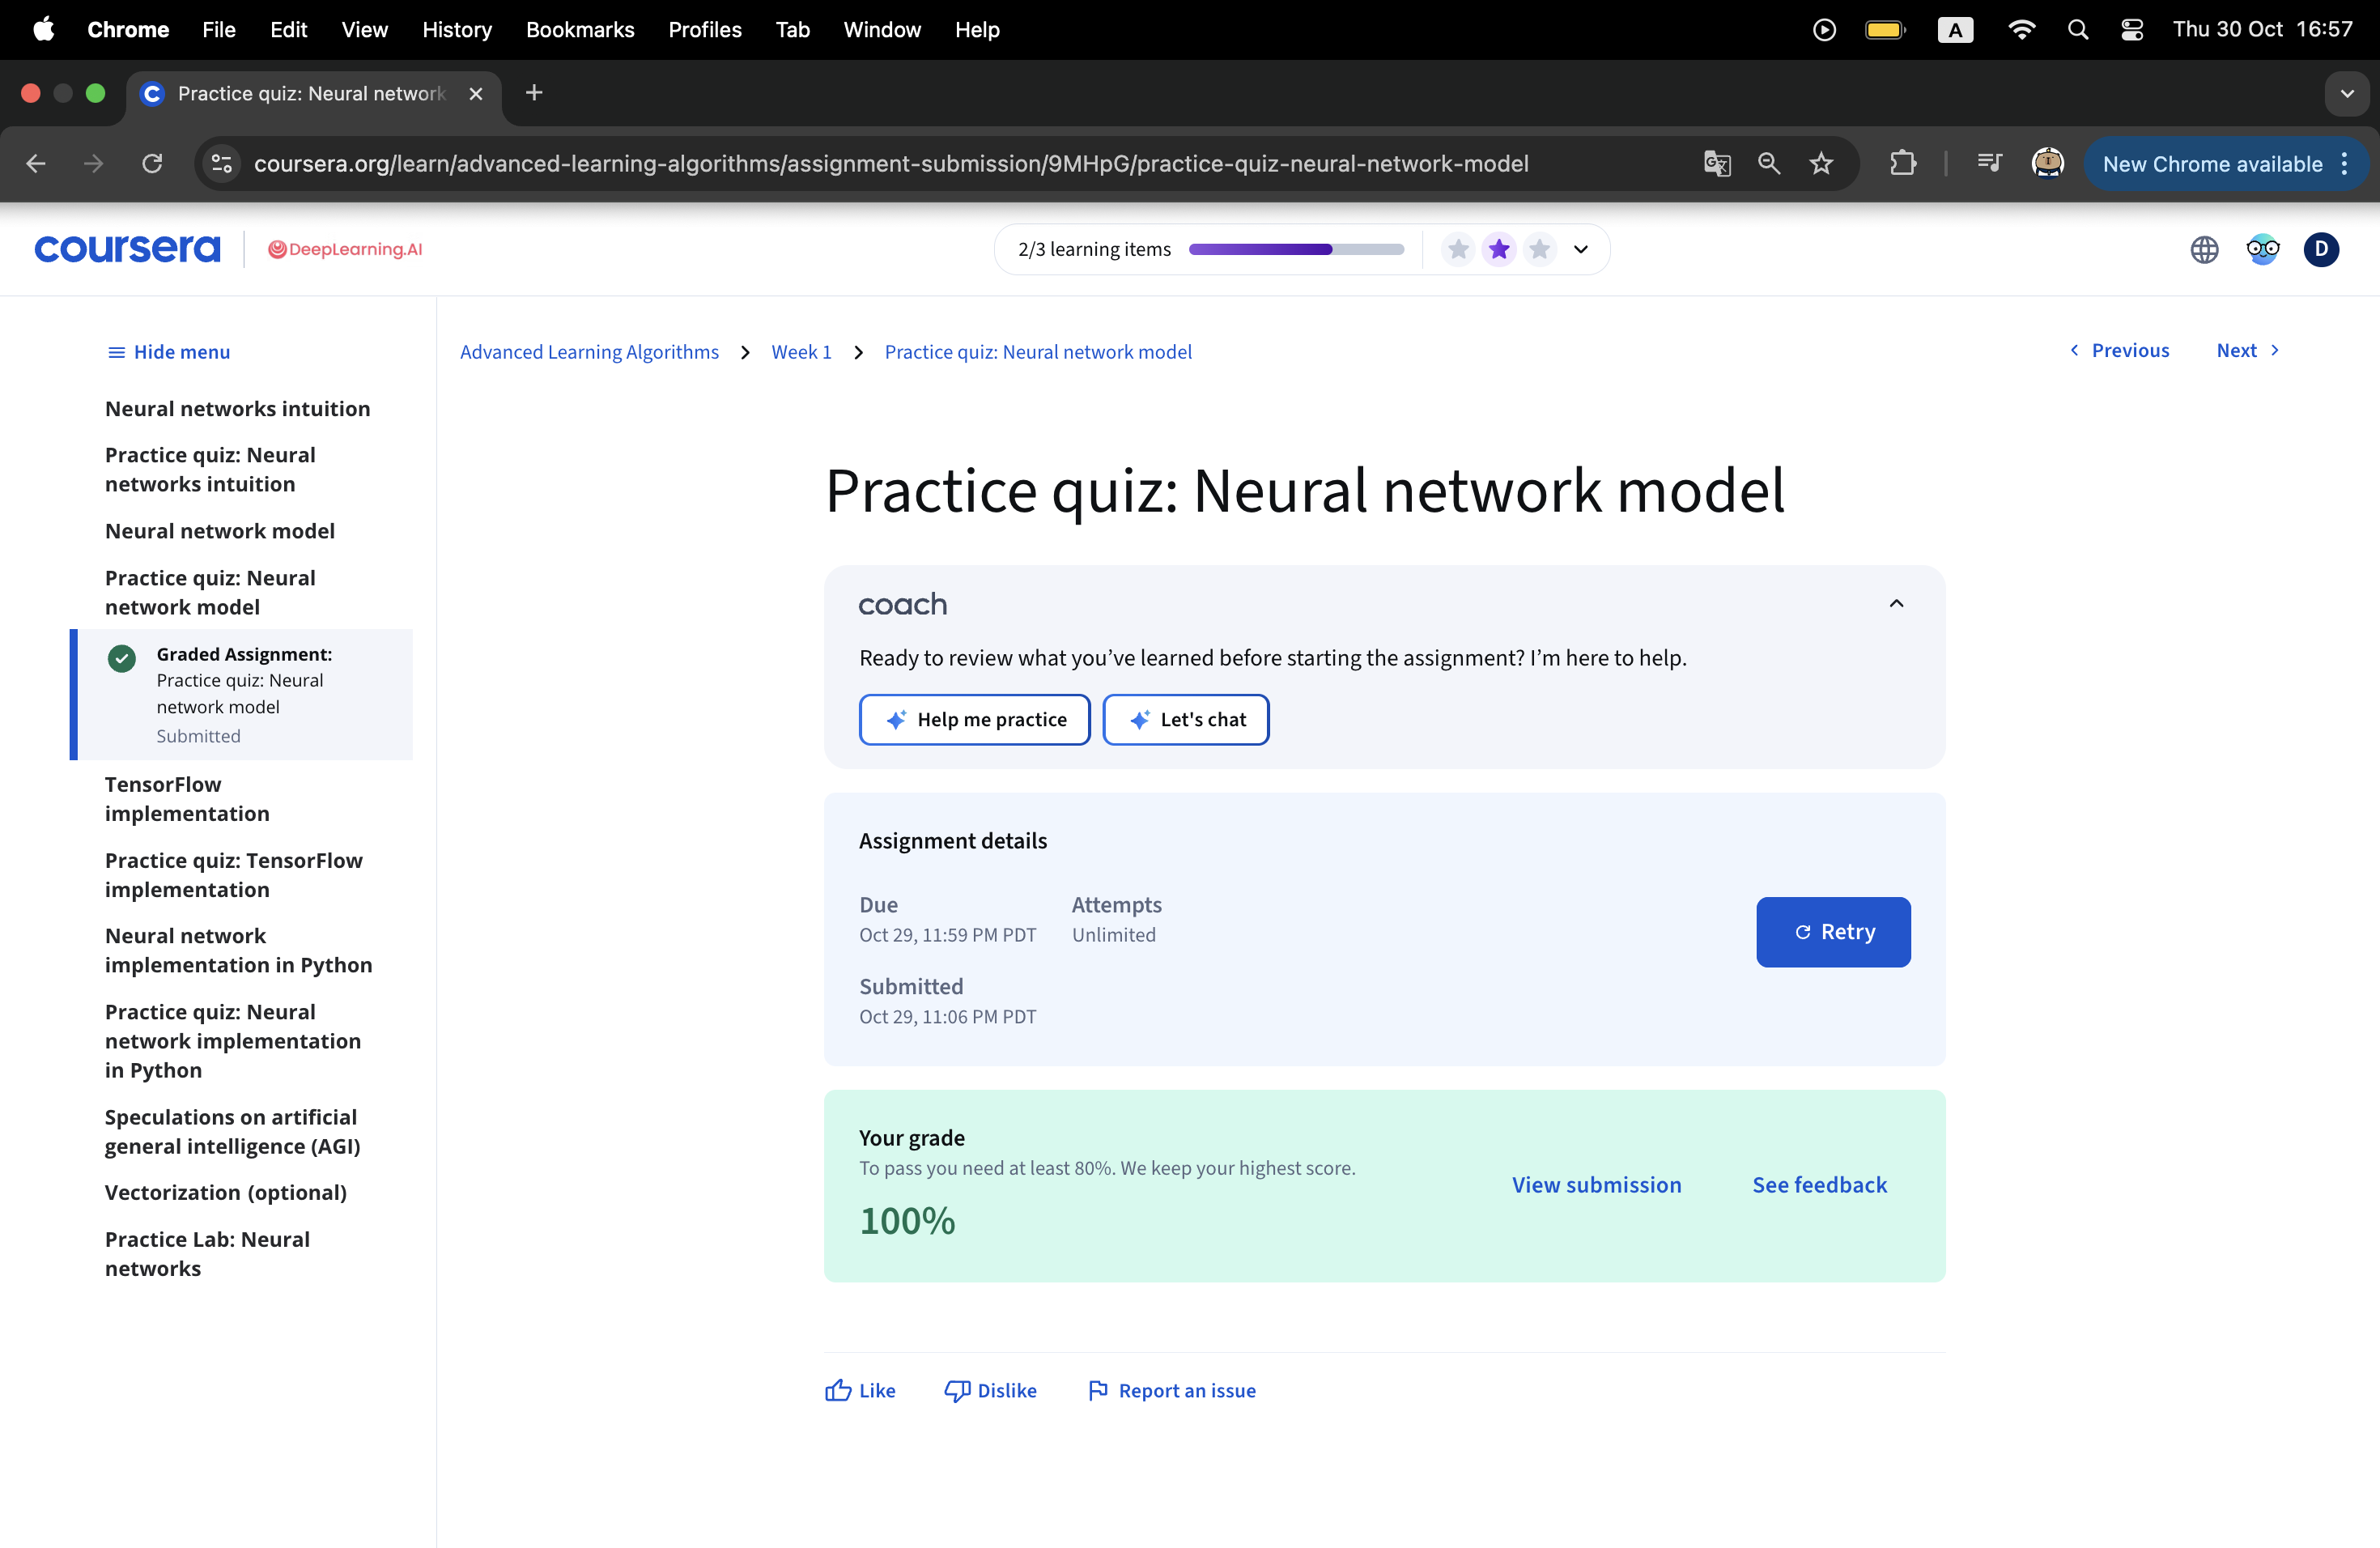
\includegraphics[scale=0.27]{Image/c2_w1_q2.png}
    \caption{Completed Graded Assignment 2 (Neural network model)}
\end{figure}

\begin{figure}[H]
    \centering
    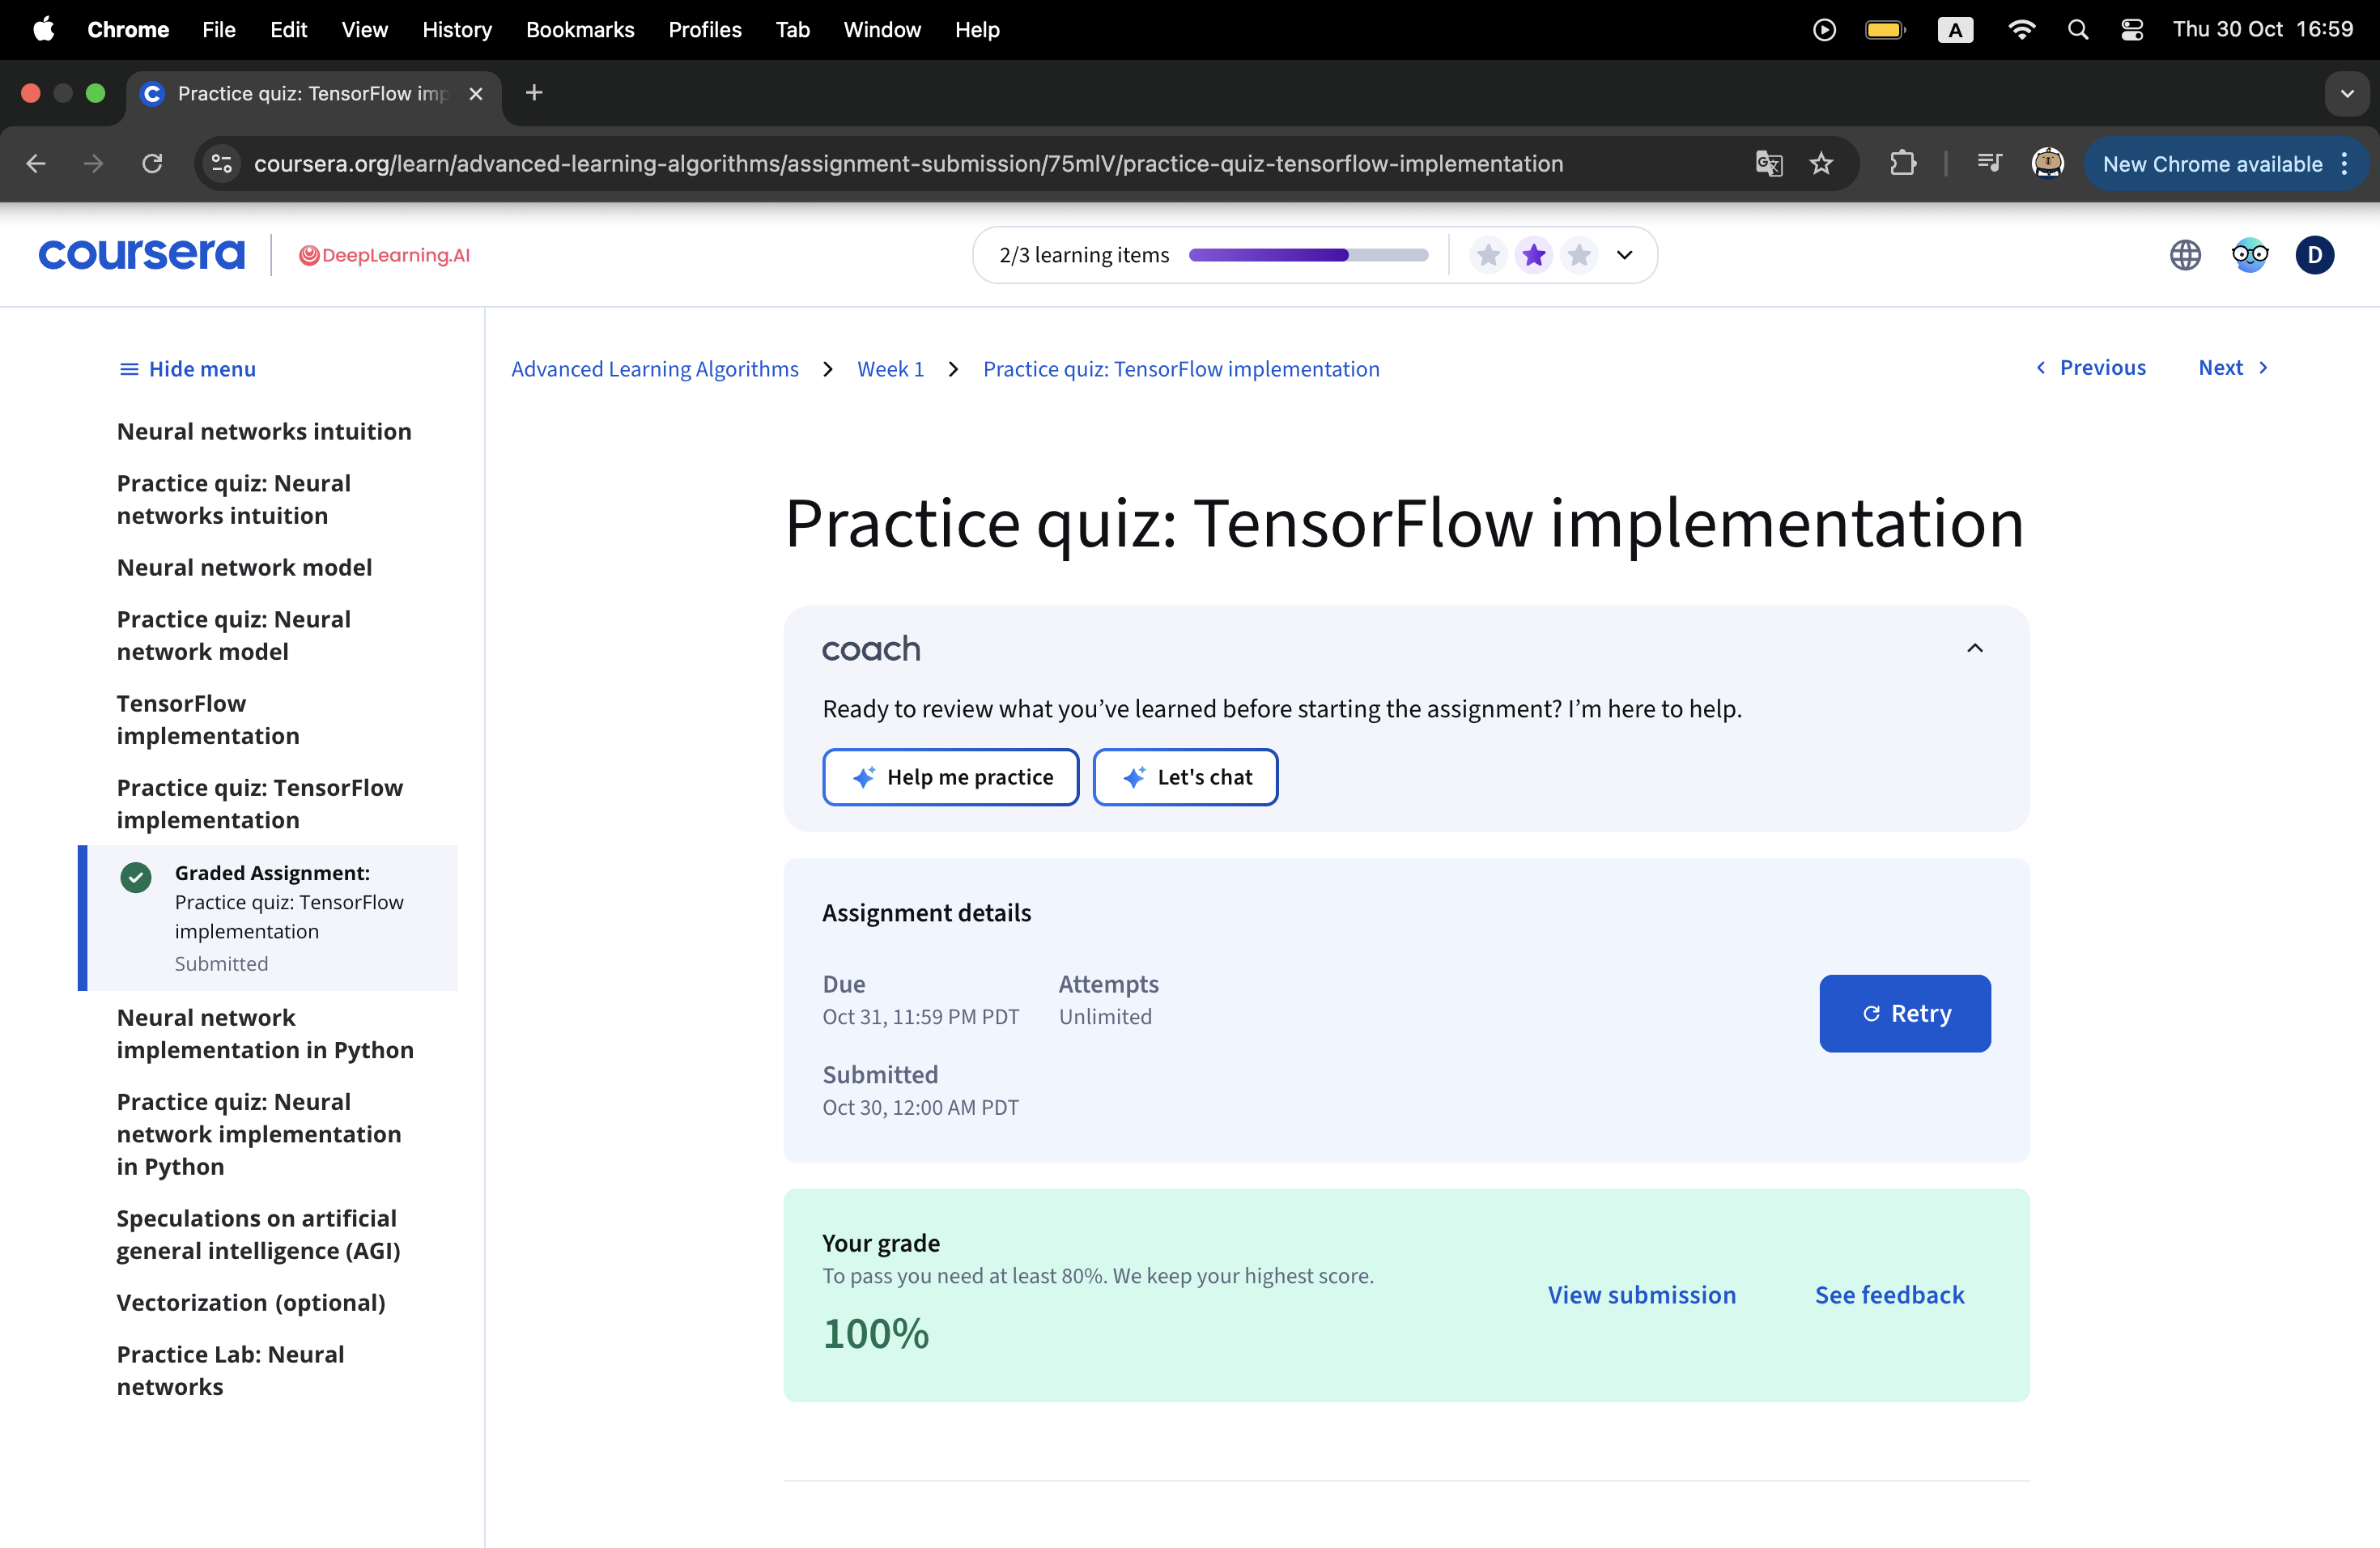
\includegraphics[scale=0.27]{Image/c2_w1_q3.png}
    \caption{Completed Graded Assignment 3 (TensorFlow implementation)}
\end{figure}

\begin{figure}[H]
    \centering
    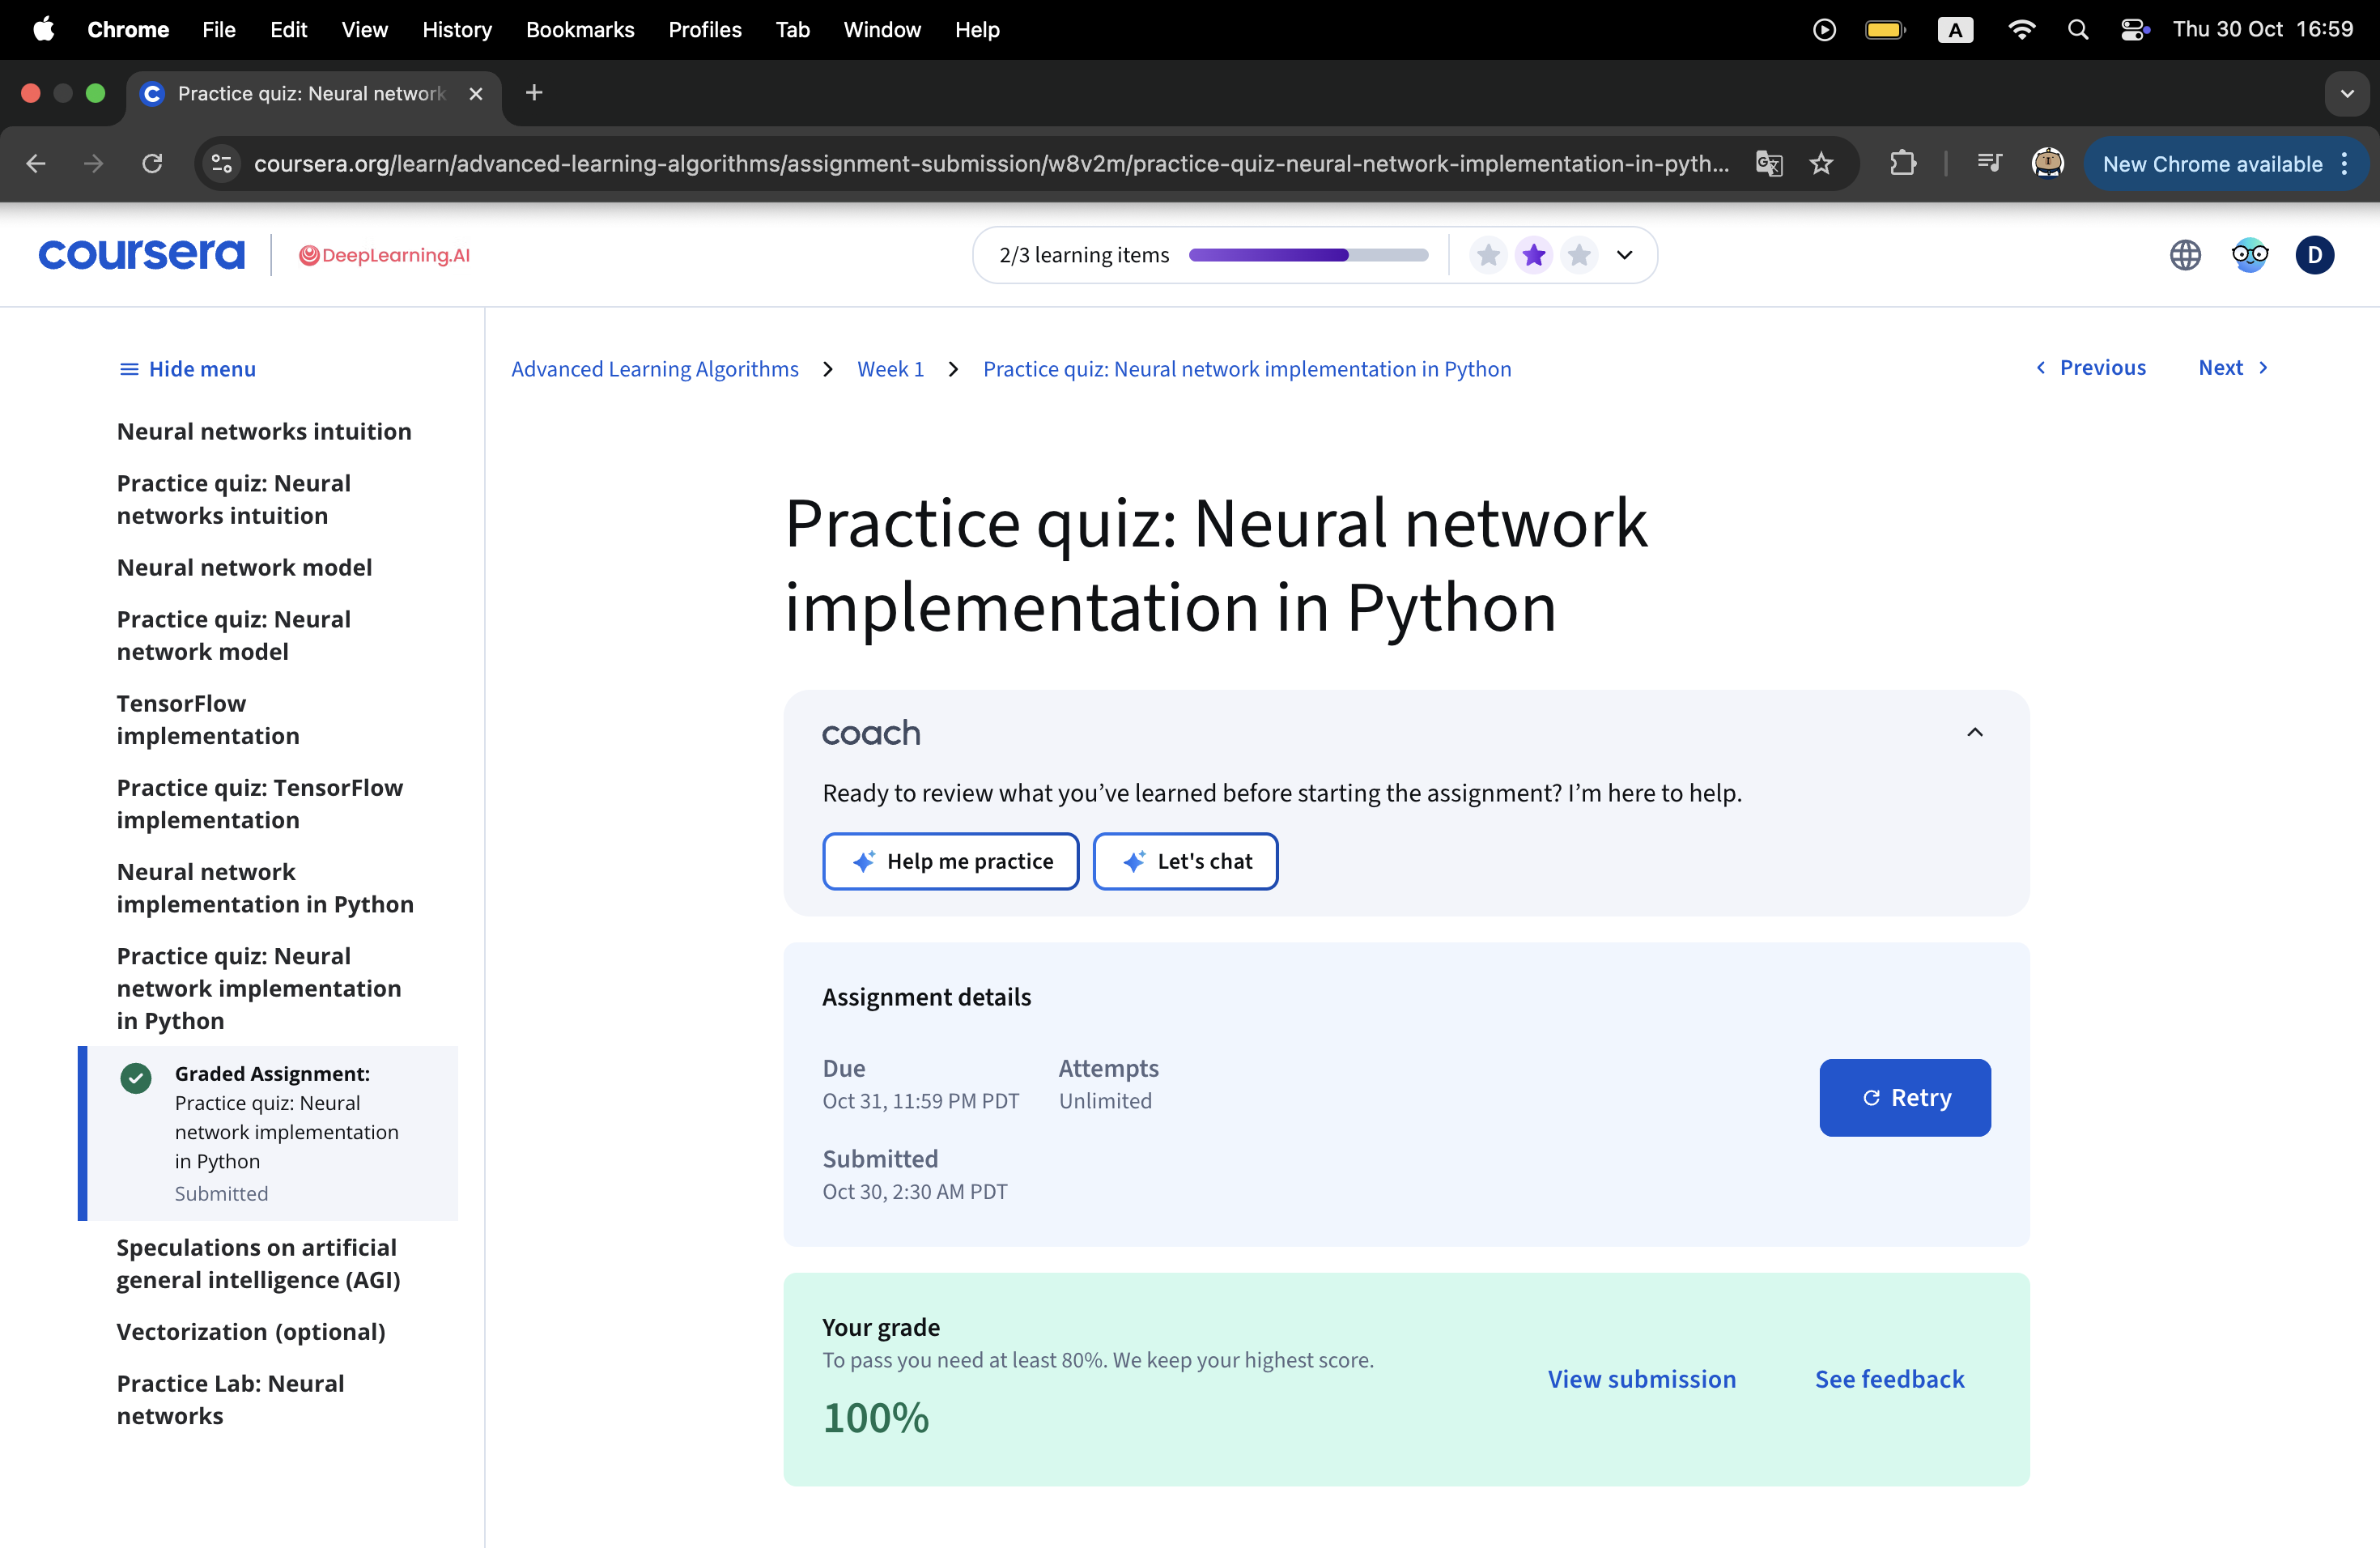
\includegraphics[scale=0.27]{Image/c2_w1_q4.png}
    \caption{Completed Graded Assignment 4 (Neural network implementation in Python)}
\end{figure}

\begin{figure}[H]
    \centering
    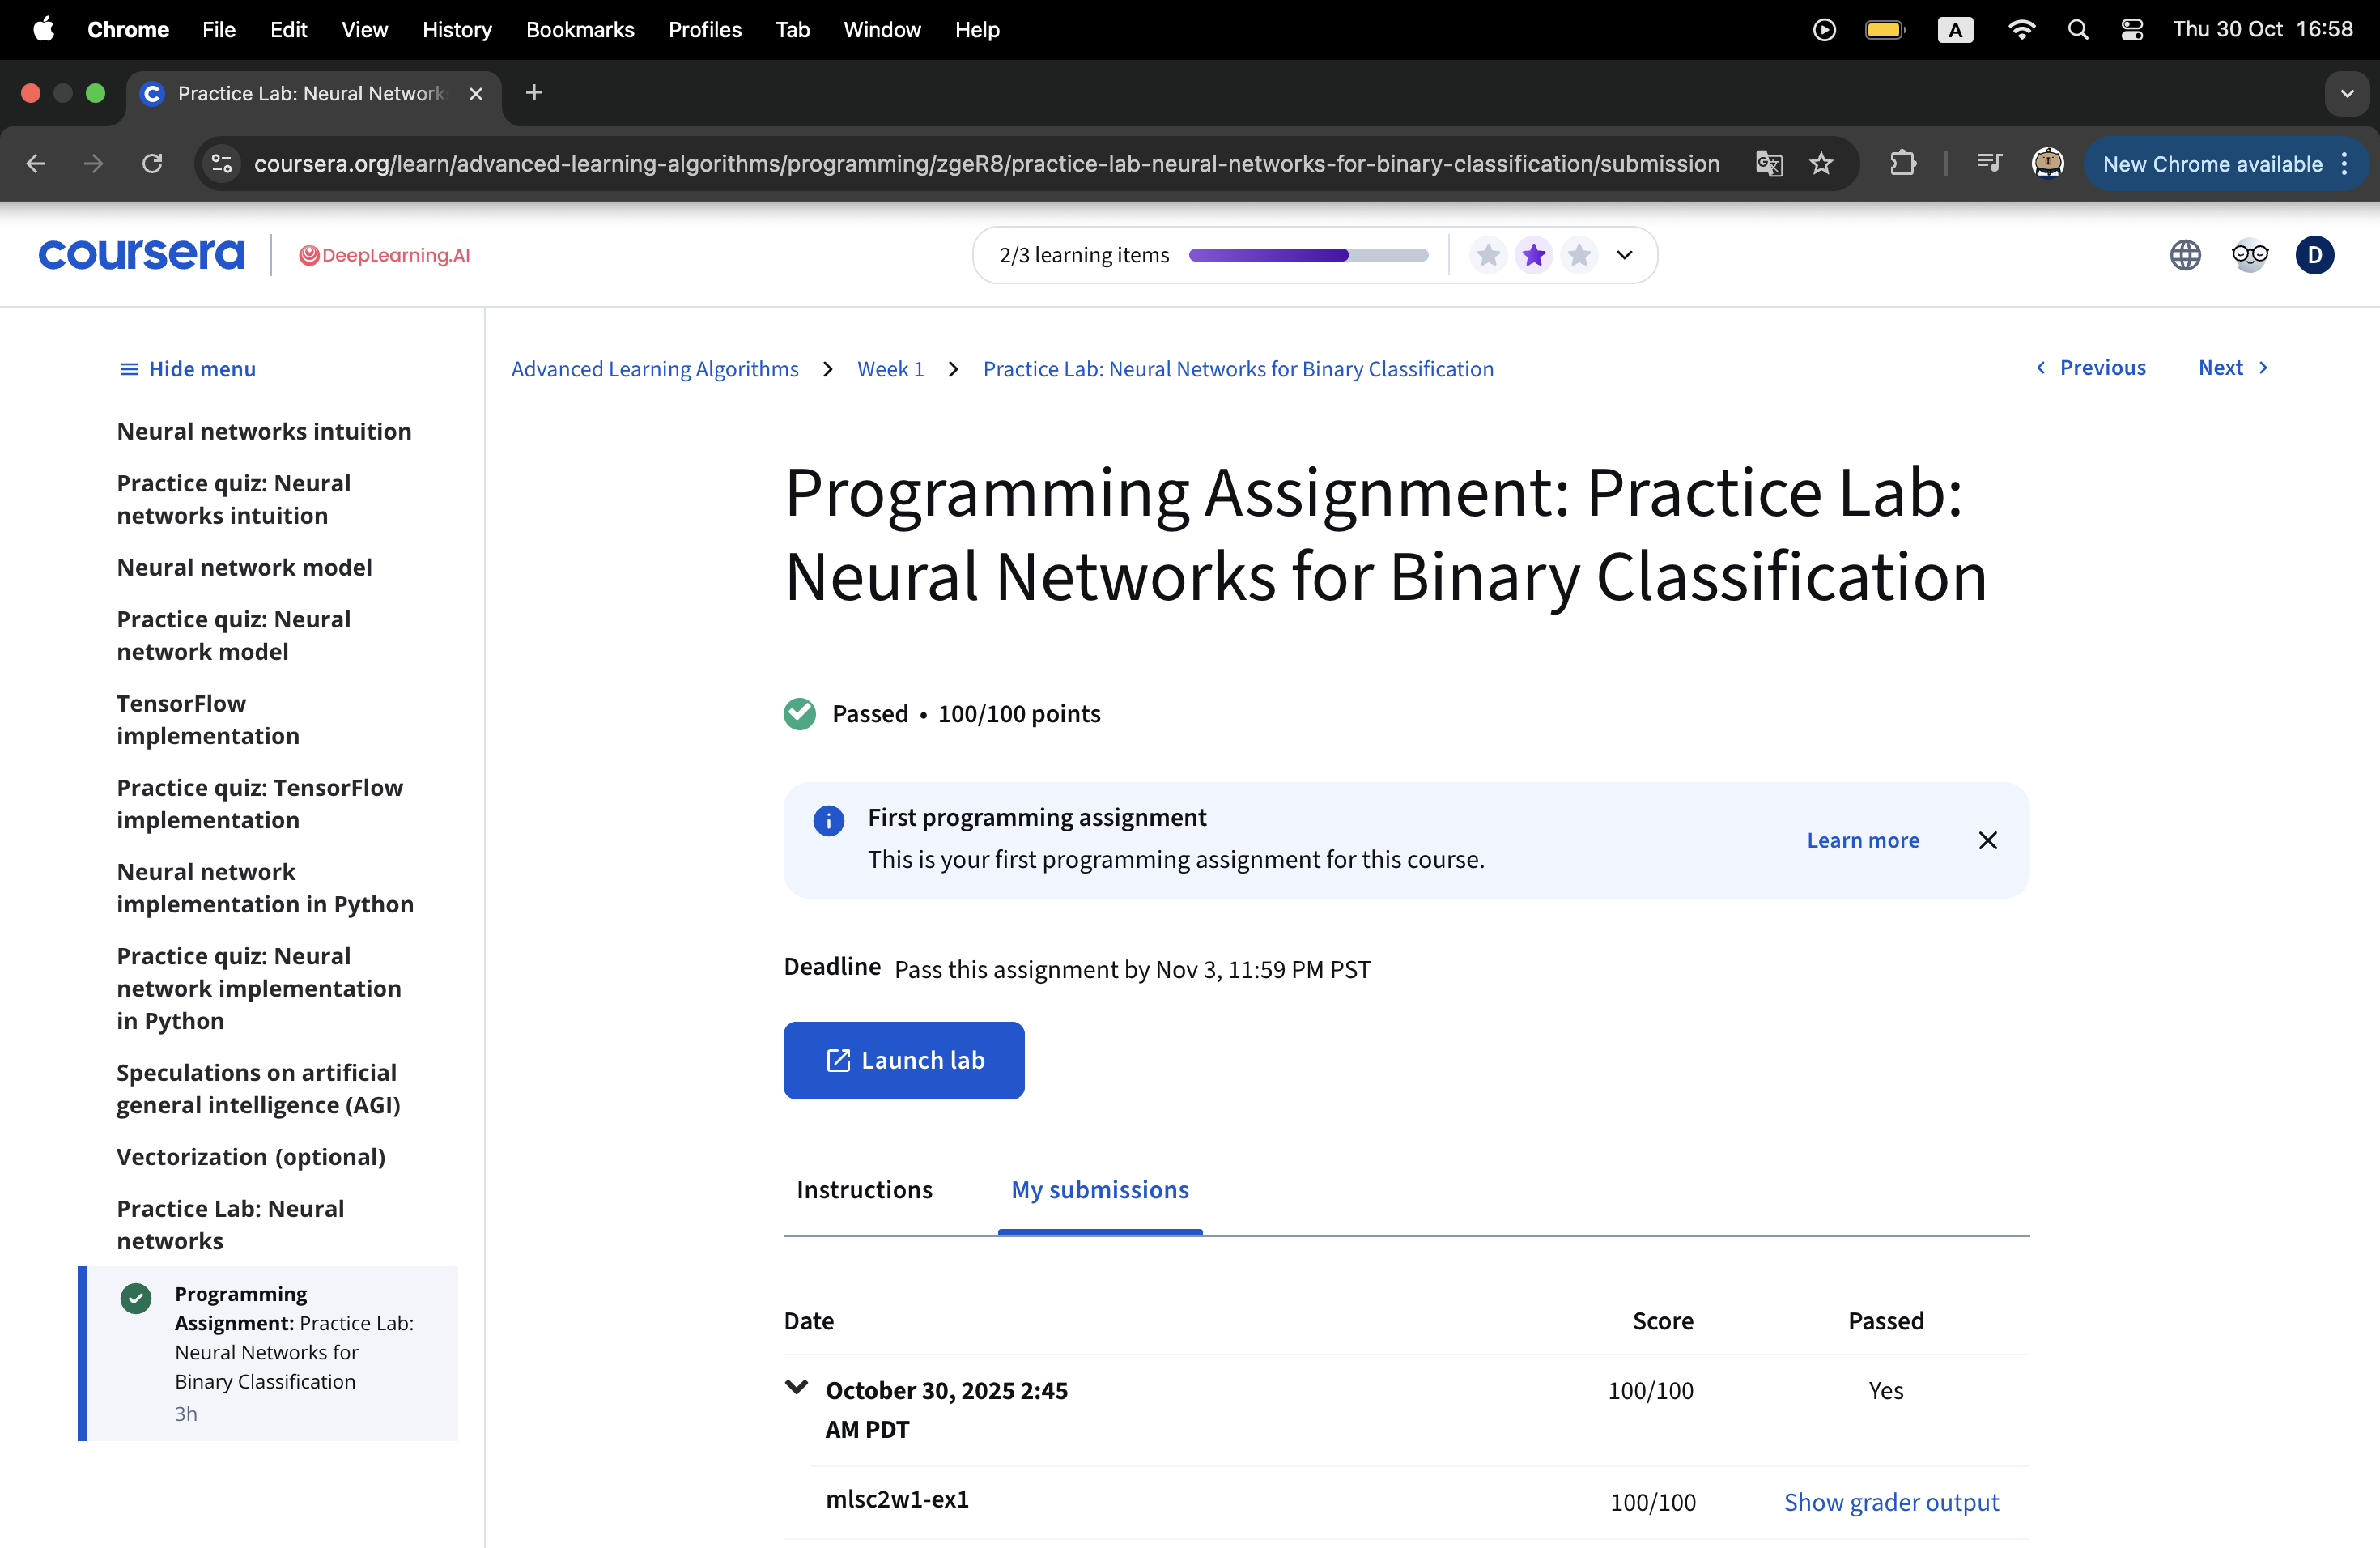
\includegraphics[scale=0.27]{Image/c2_w1_q5.png}
    \caption{Completed Programming Assignment (Neural Networks for Binary Classification)}
\end{figure}

%----------------------------------------
\subsection{Week 2: Neural Network Training}
%----------------------------------------

\subsubsection{Key Insights and Learnings}

This module demystified the "black box" of training, focusing on the mathematical optimization and advanced techniques required for convergence.

\begin{itemize}
    \item \textbf{Backpropagation Algorithm:} Mastered the chain rule application in computation graphs. This algorithm efficiently computes the partial derivatives ($\frac{\partial J}{\partial w}$) of the cost function, guiding the network on how to adjust weights to minimize error.
    
    \item \textbf{Advanced Optimization:} 
    \begin{itemize}
        \item Moved beyond standard Gradient Descent to \textbf{Adam (Adaptive Moment Estimation)}.
        \item \textbf{Adam} adjusts learning rates individually for each parameter, resulting in faster convergence and better handling of local optima compared to standard SGD.
    \end{itemize}

    \item \textbf{Handling Overfitting (Regularization):} Implemented strategies to improve model generalization:
    \begin{itemize}
        \item \textbf{L2 Regularization:} Penalizing large weights in the cost function.
        \item \textbf{Dropout:} Randomly deactivating neurons during training to prevent over-reliance on specific features.
    \end{itemize}
\end{itemize}

\subsubsection{Learning Evidence}
\begin{figure}[H]
    \centering
    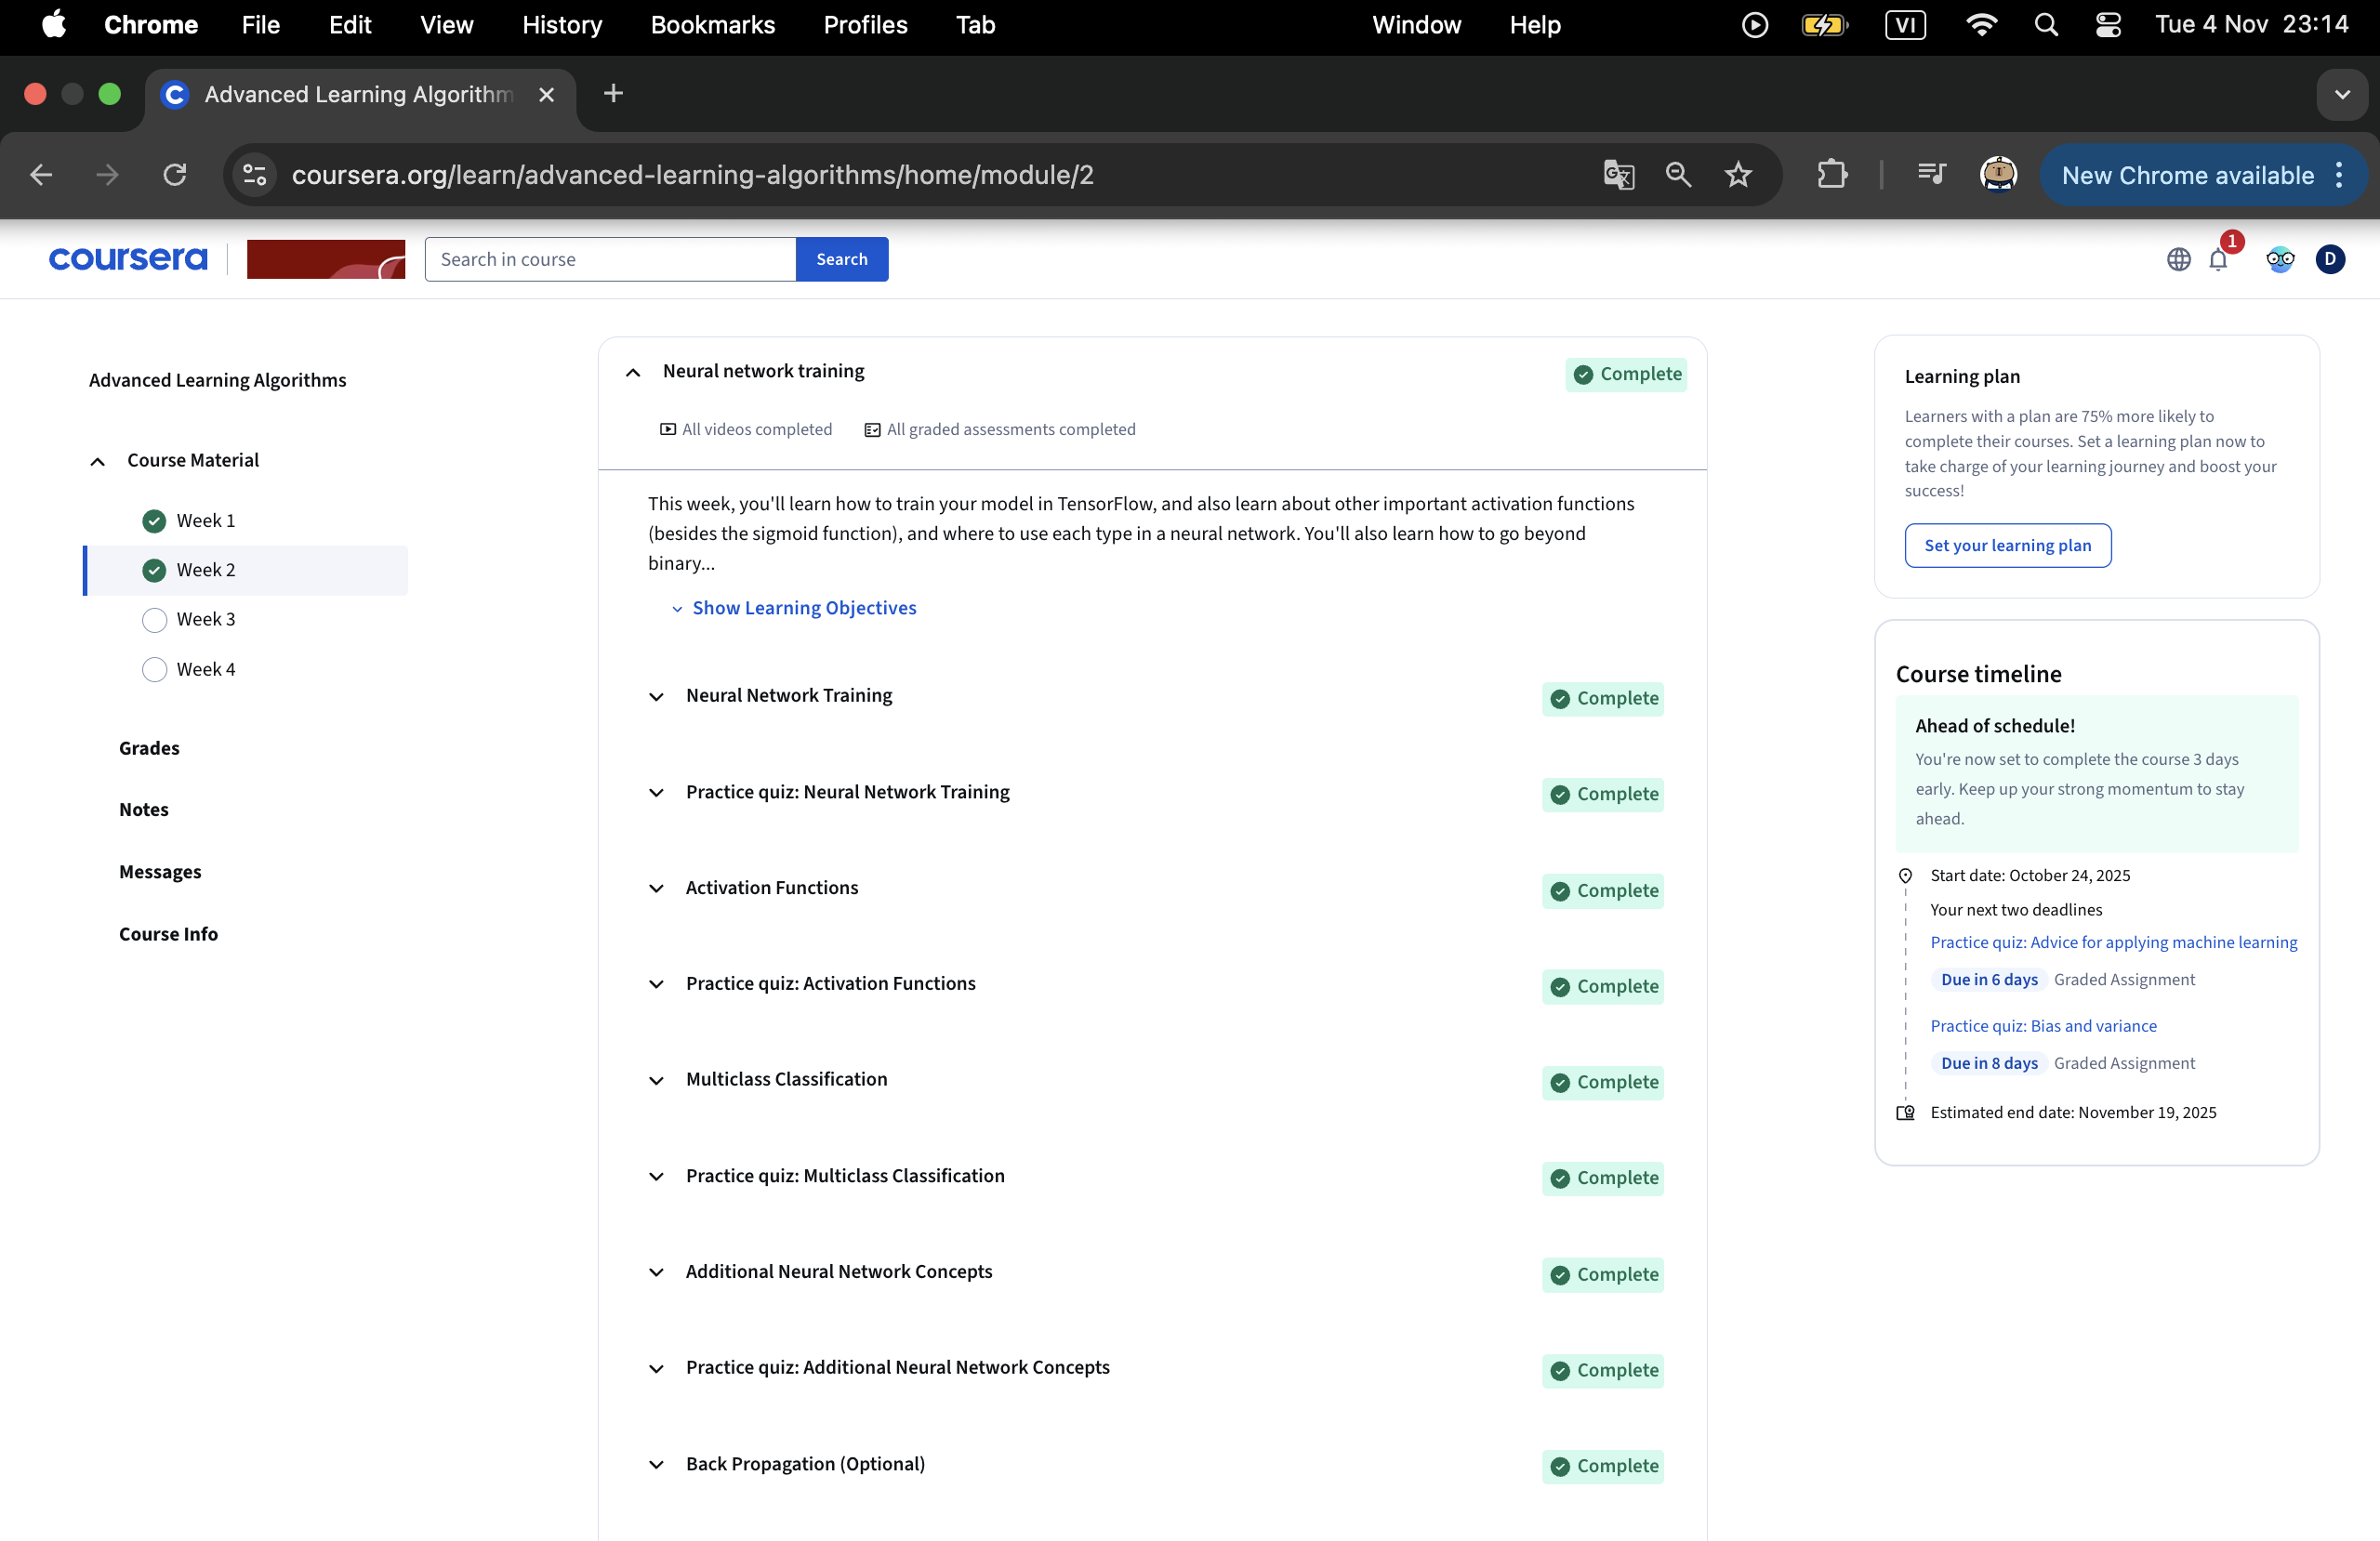
\includegraphics[scale=0.27]{Image/c2_w2.png}
    \caption{Lesson's completed date (04/11/2025)}
\end{figure}

\subsubsection{Graded Assignment Evidence}
\begin{figure}[H]
    \centering
    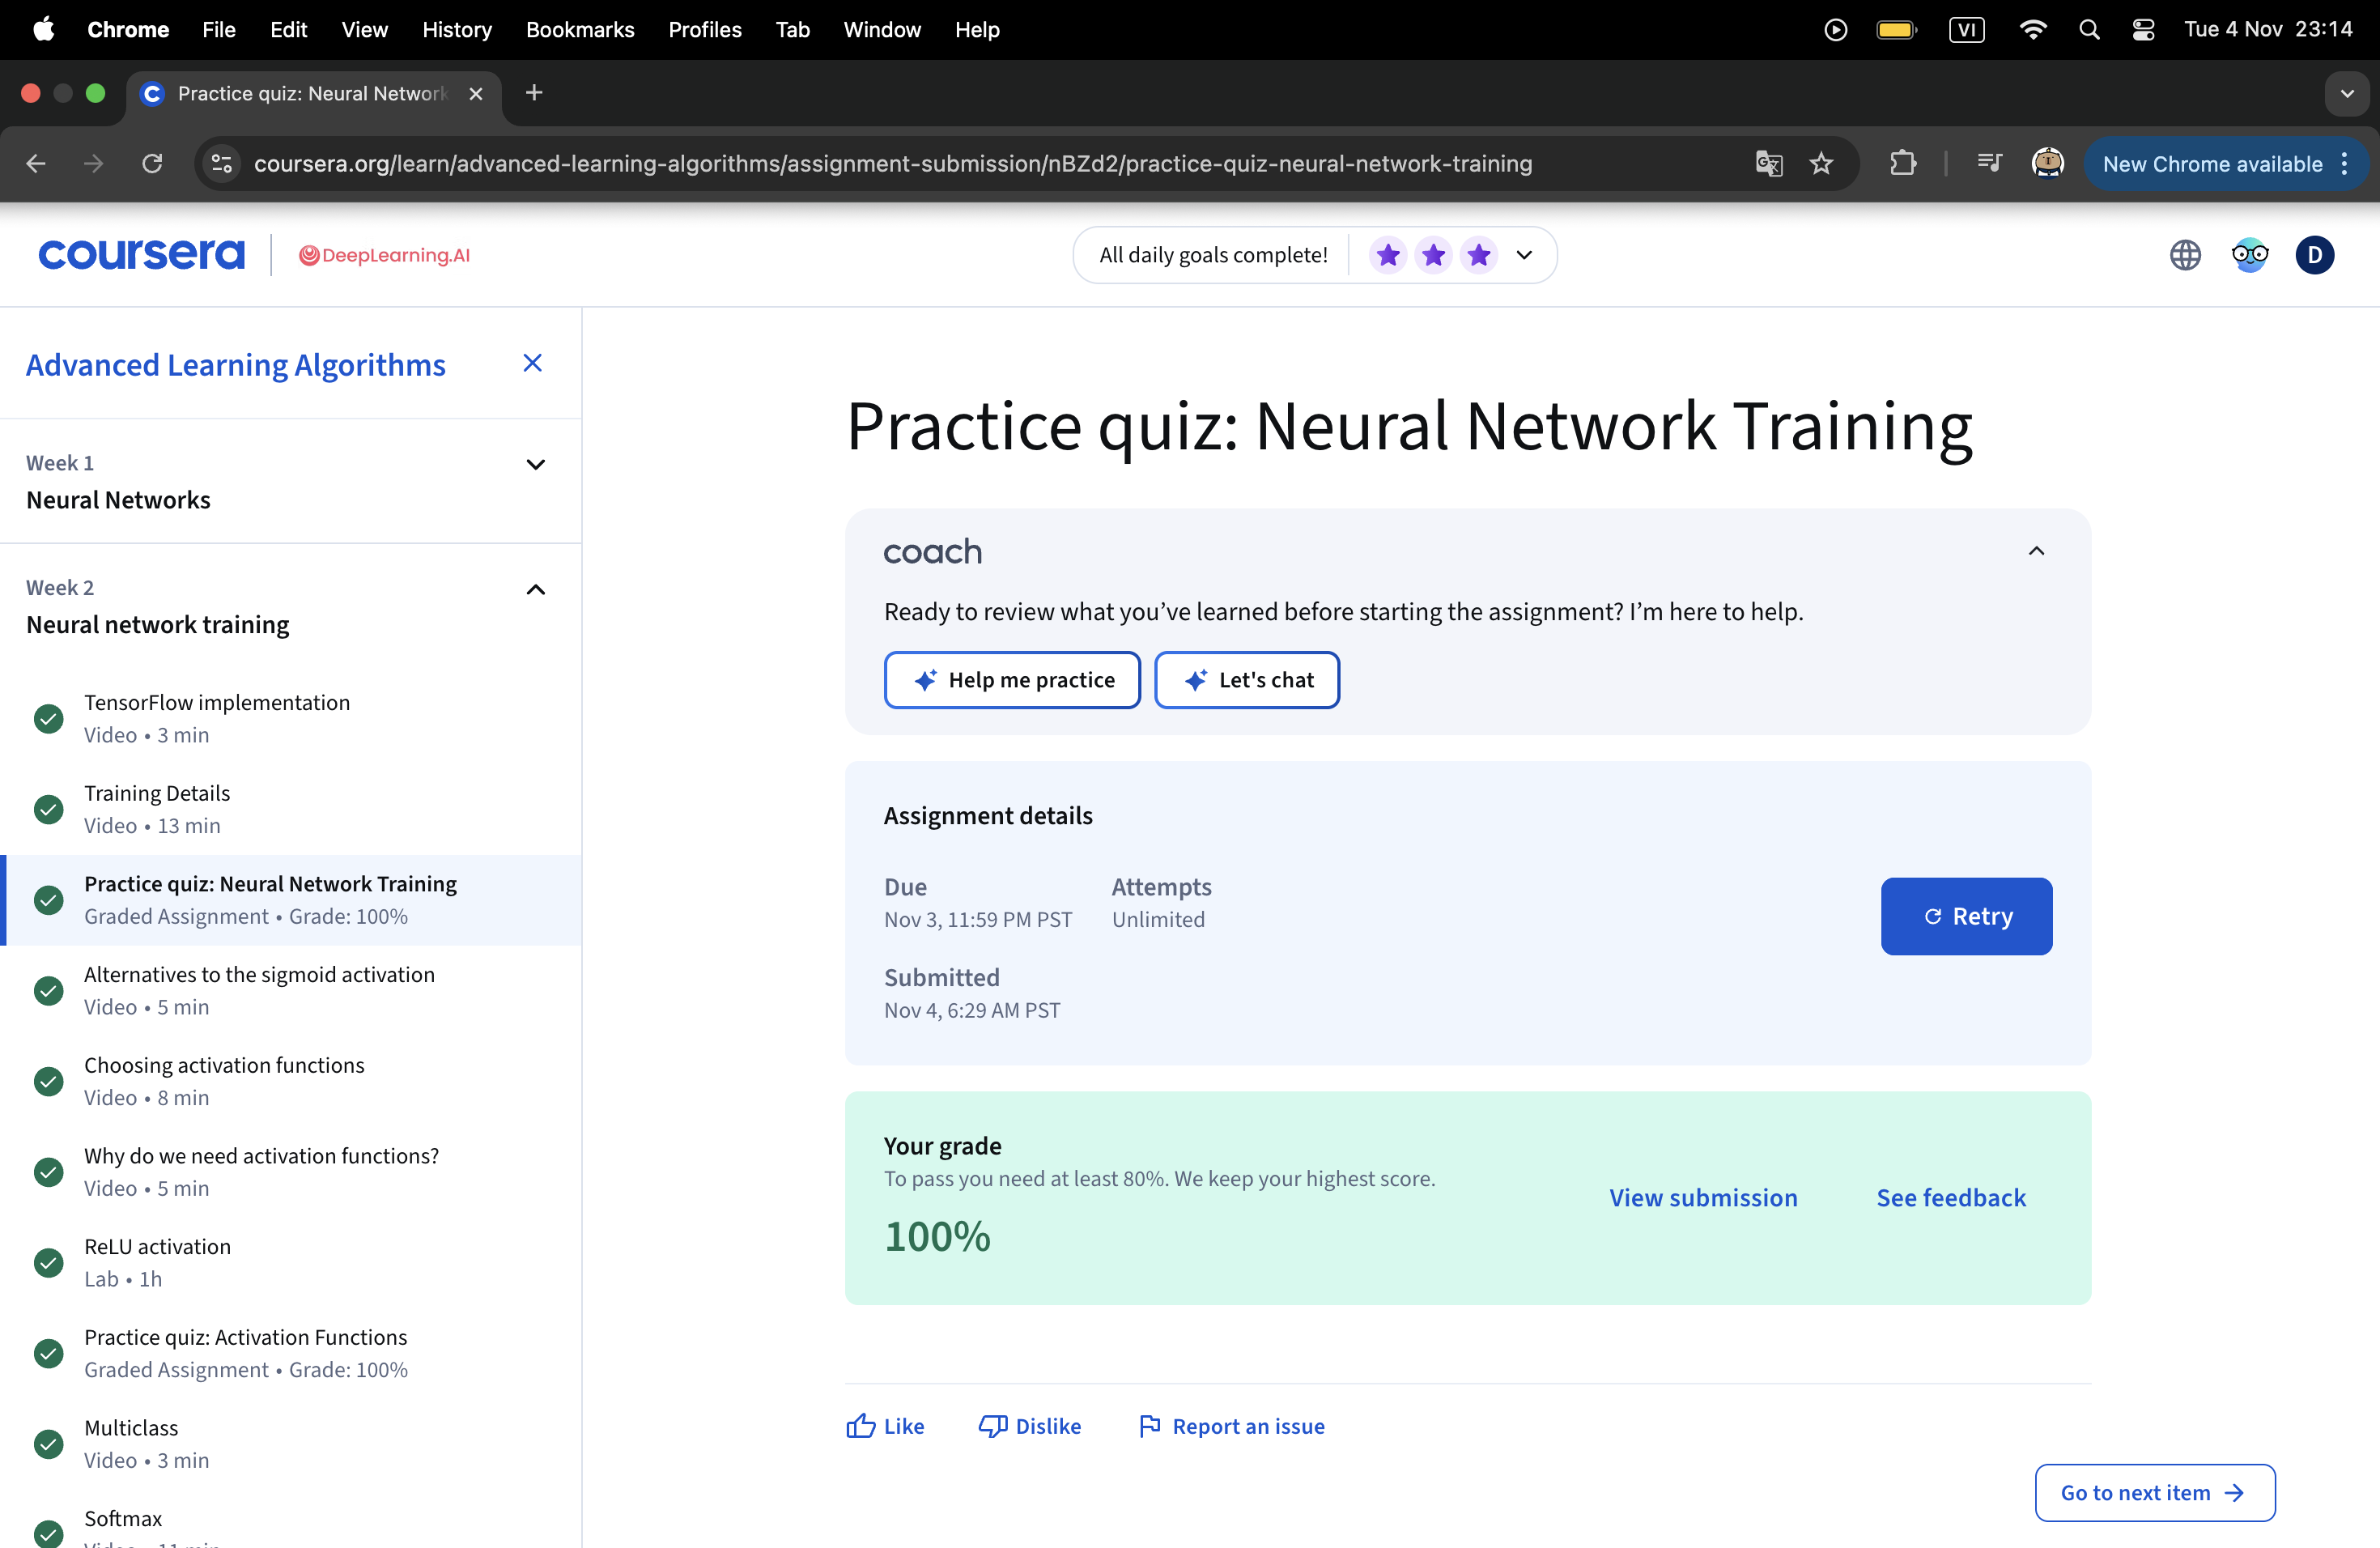
\includegraphics[scale=0.25]{Image/c2_w2_q1.png}
    \caption{Completed Graded Assignment 1 (Neural Network Training)}
\end{figure}

\begin{figure}[H]
    \centering
    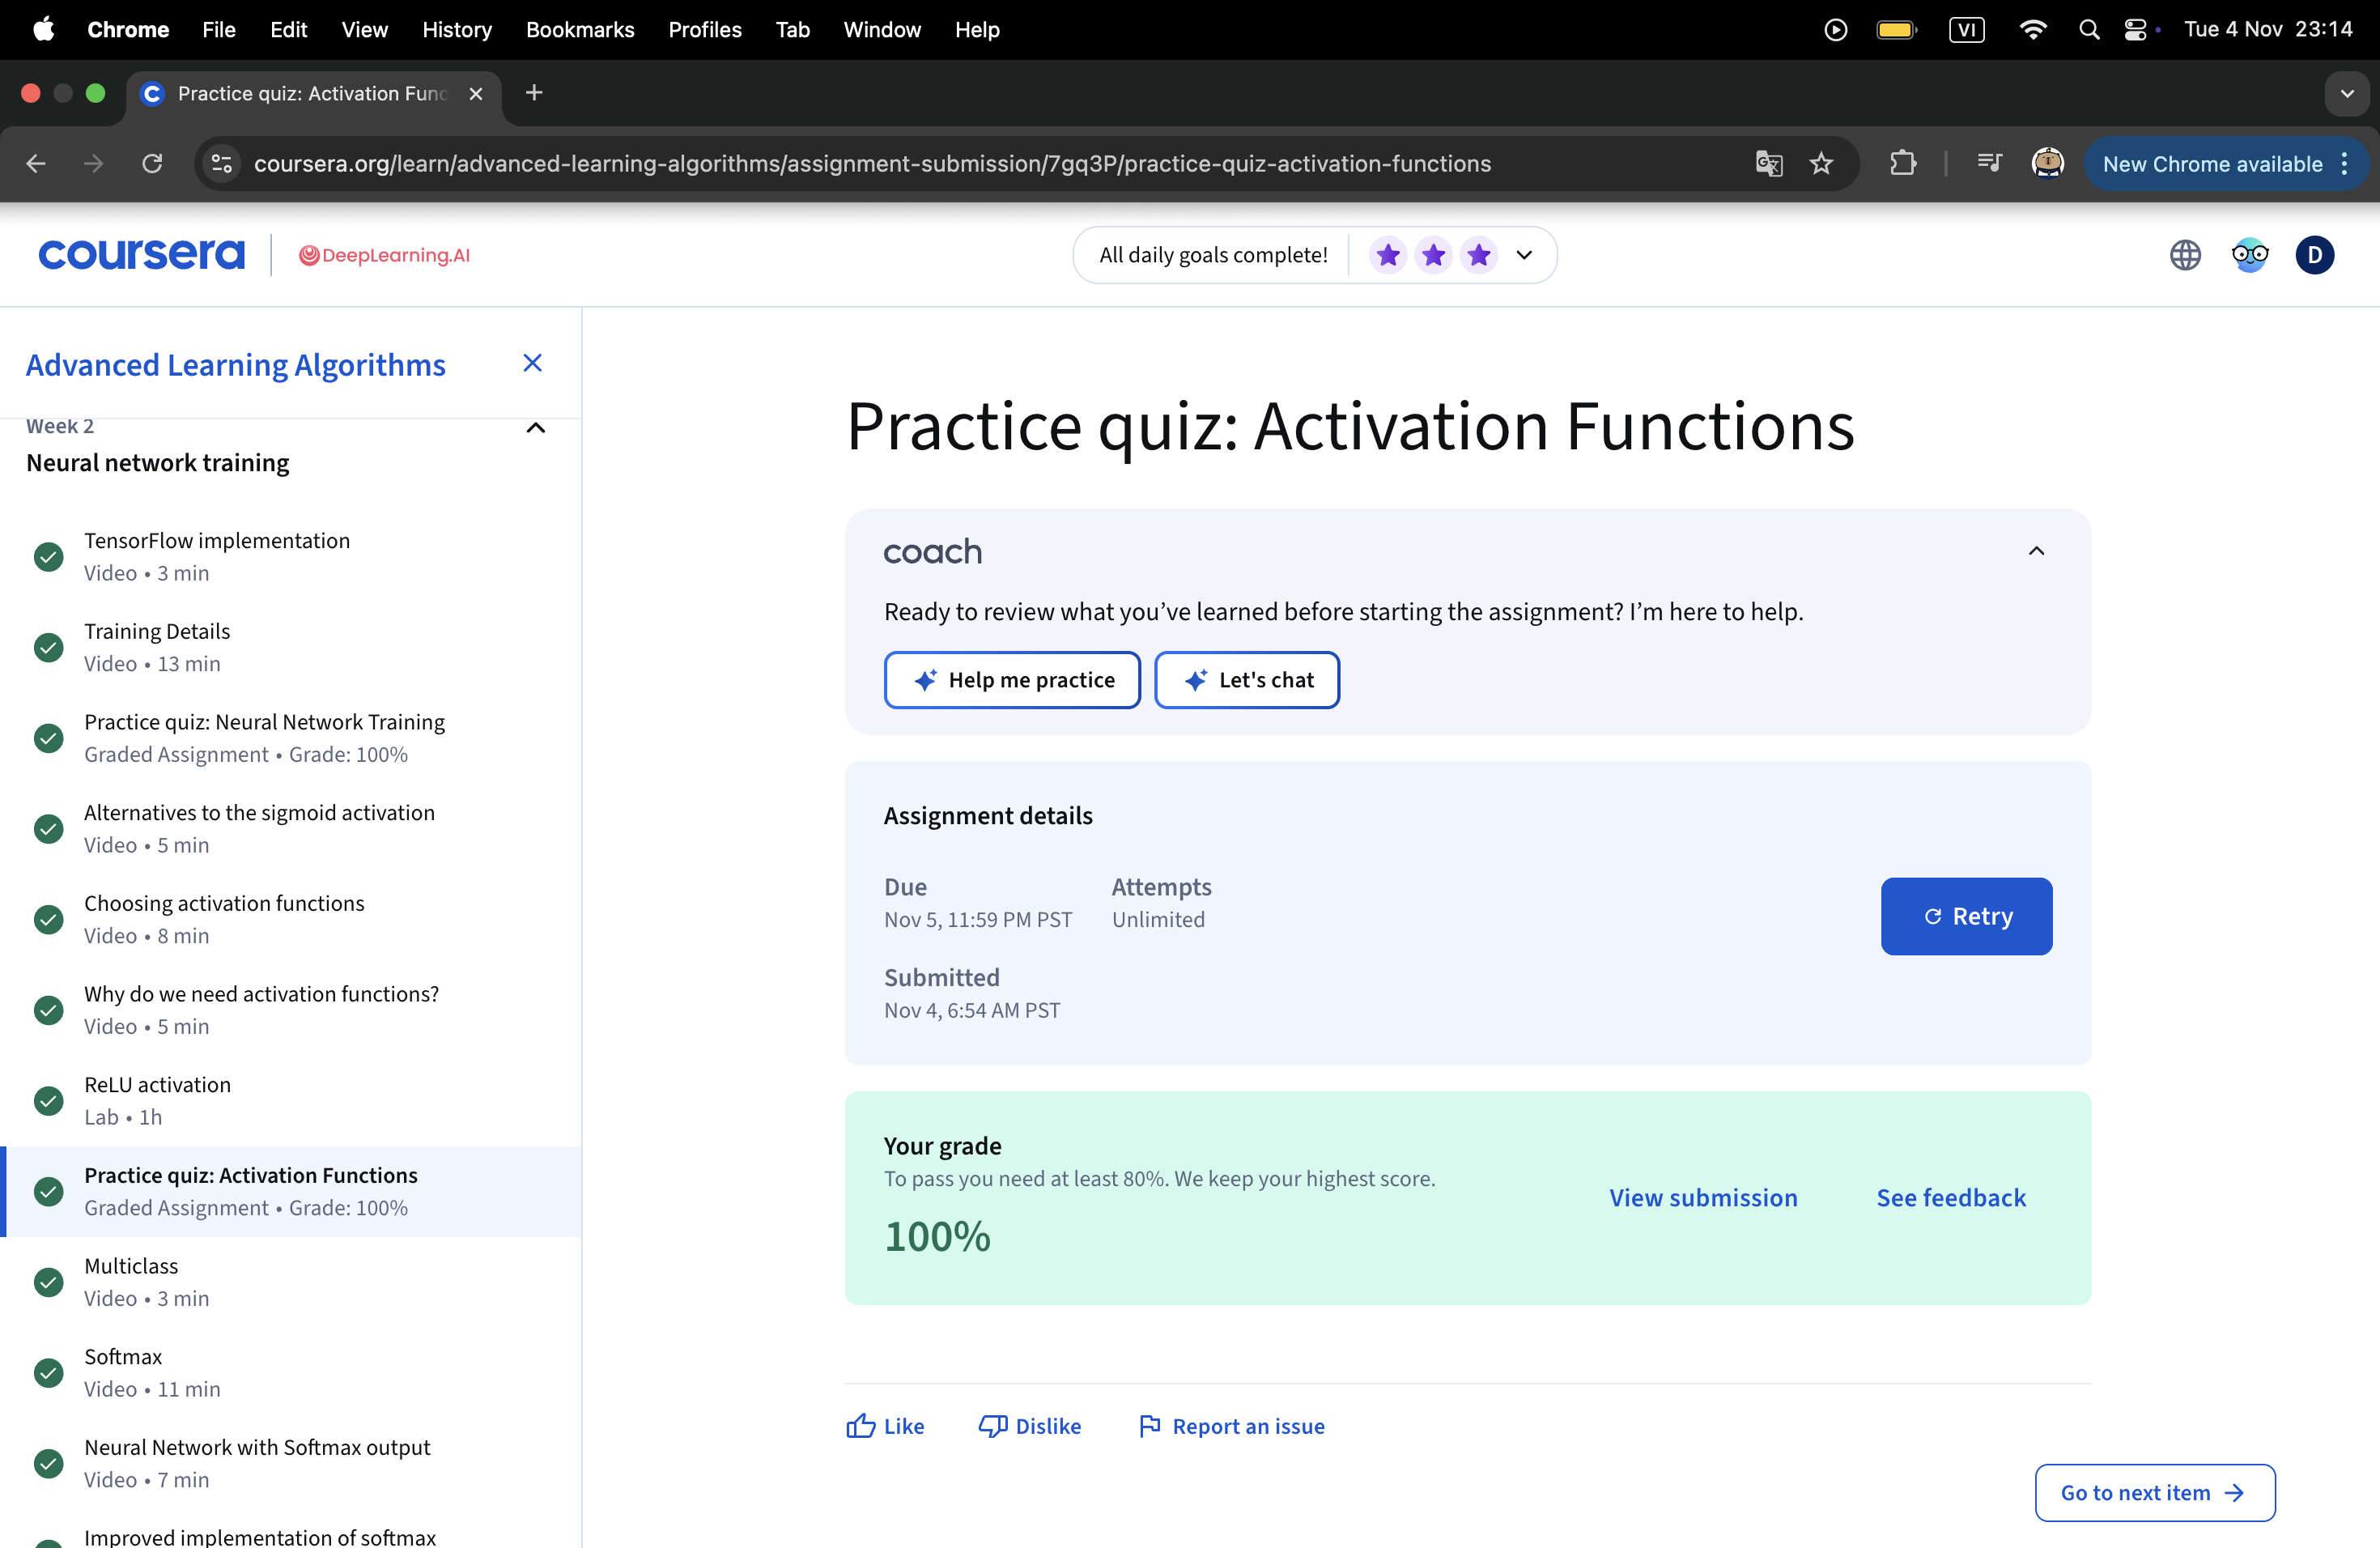
\includegraphics[scale=0.27]{Image/c2_w2_q2.png}
    \caption{Completed Graded Assignment 2 (Activation Functions)}
\end{figure}

\begin{figure}[H]
    \centering
    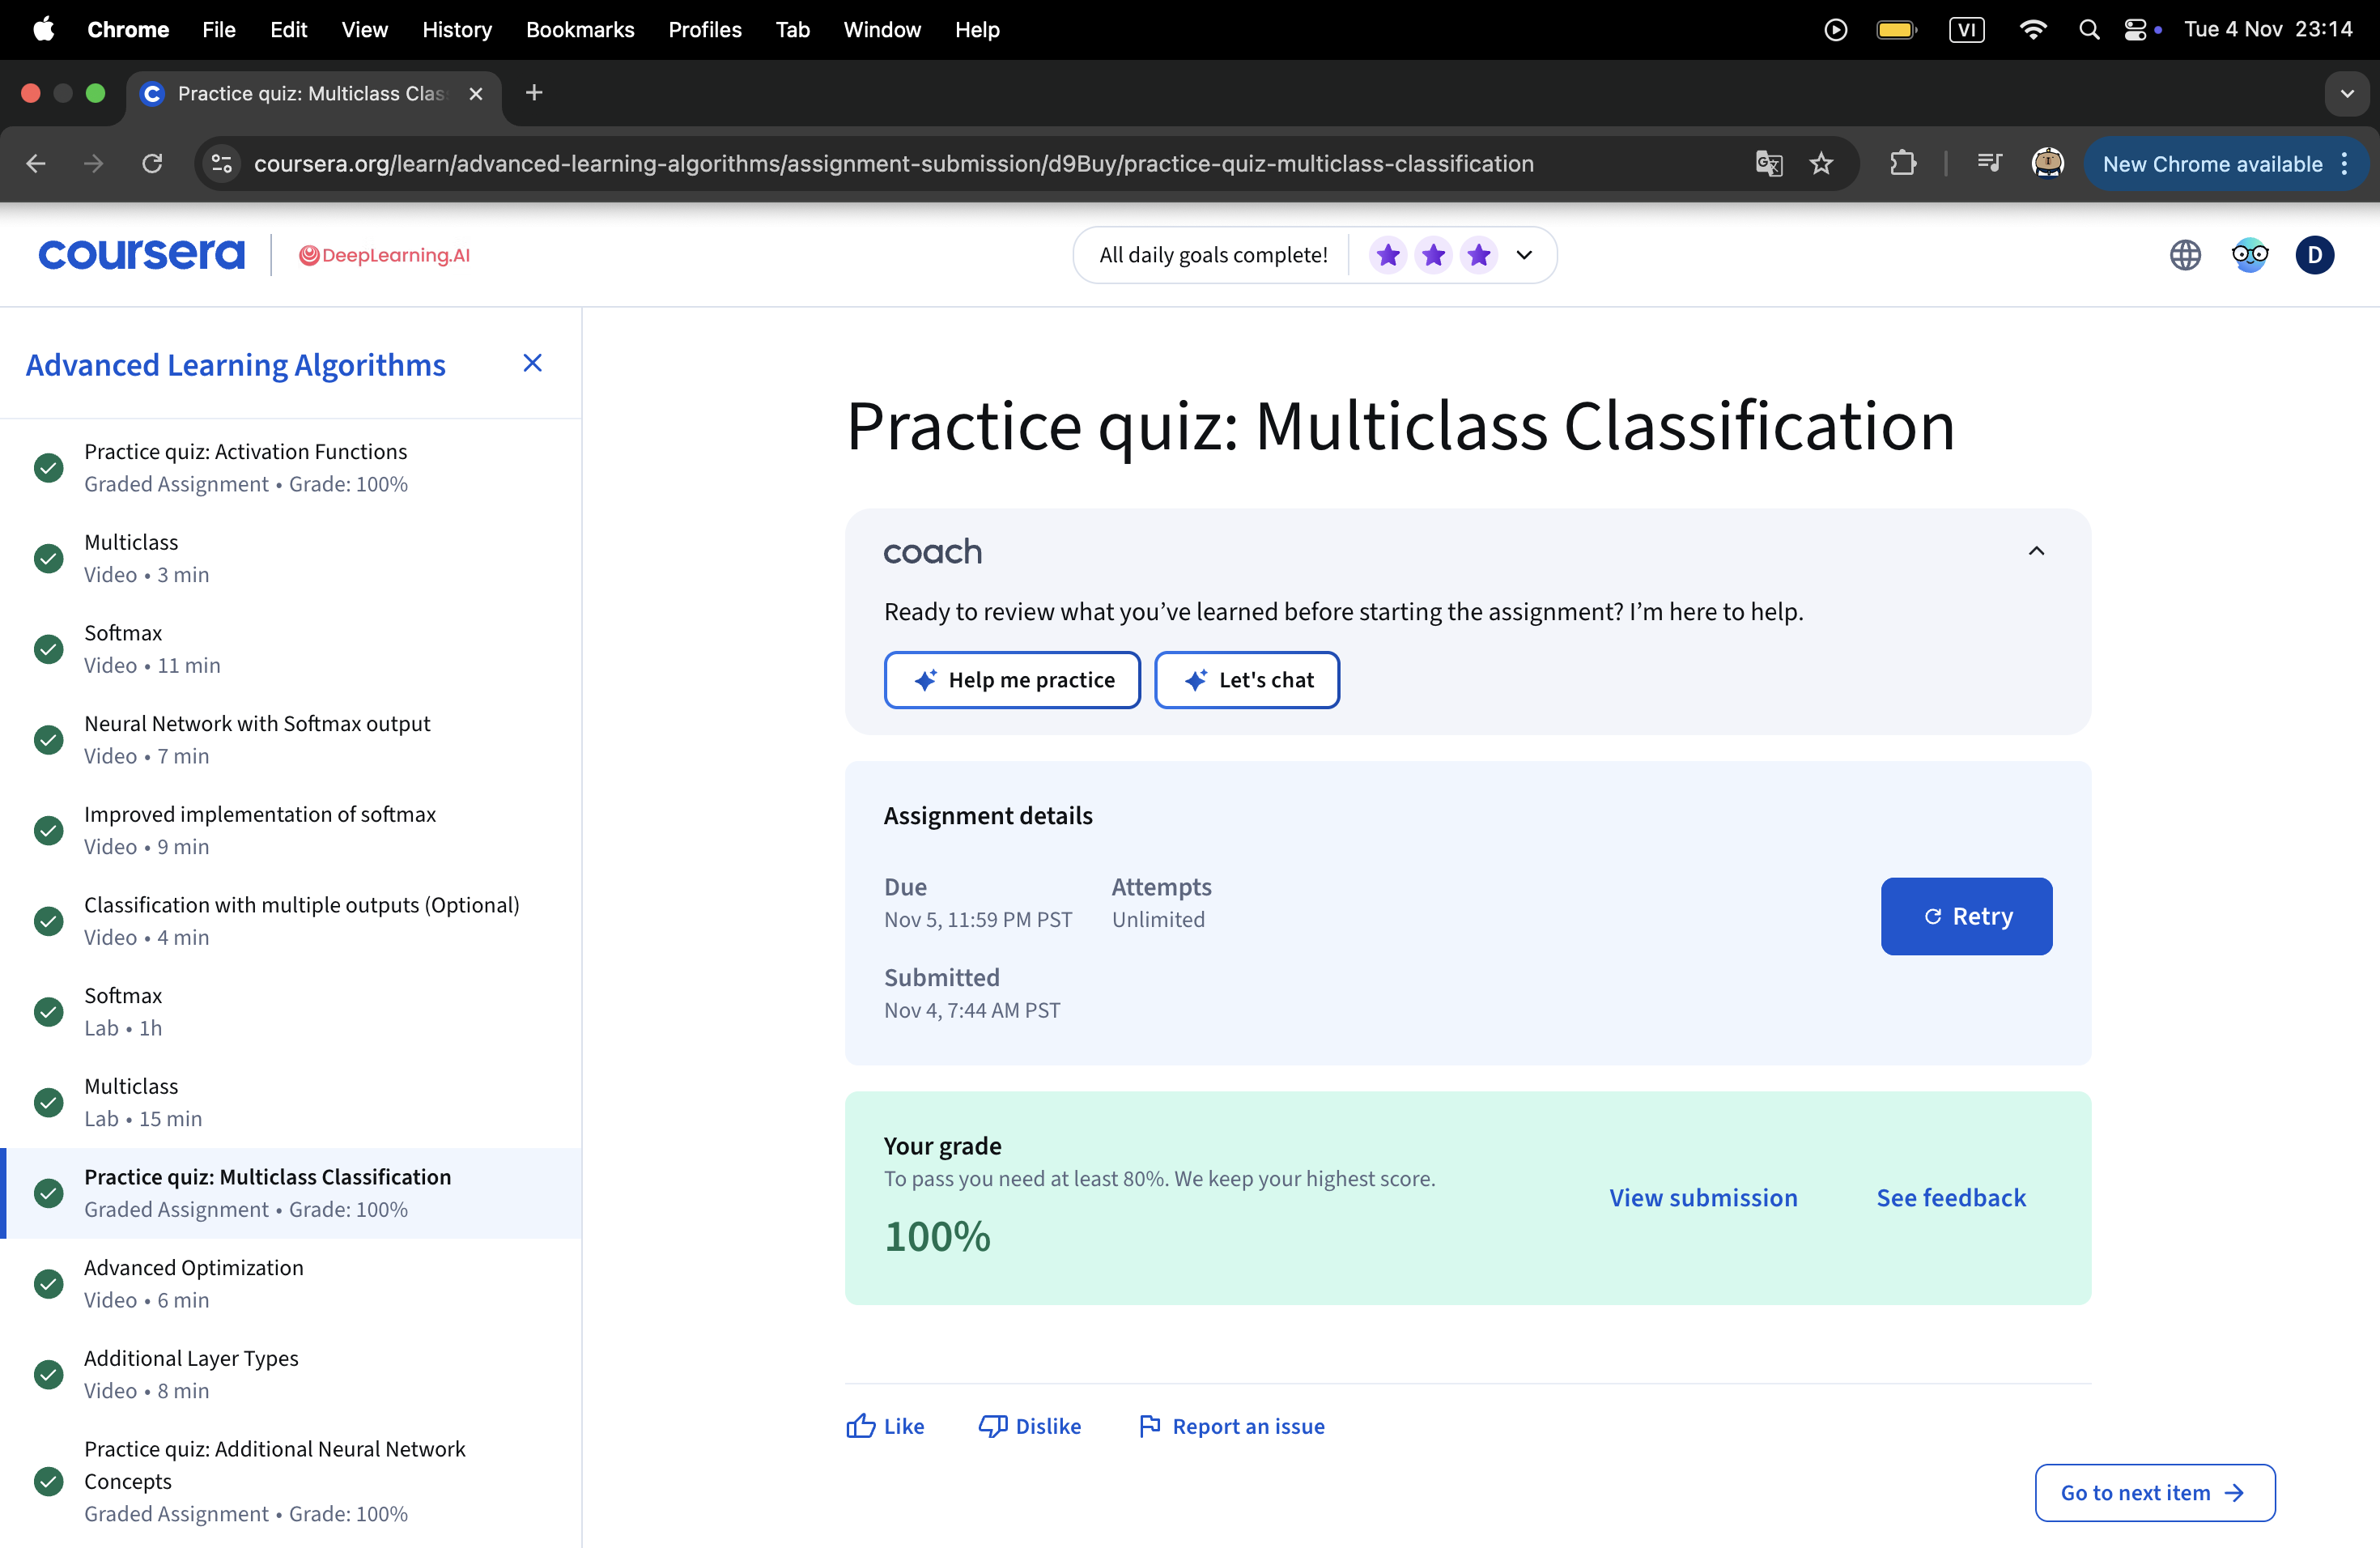
\includegraphics[scale=0.27]{Image/c2_w2_q3.png}
    \caption{Completed Graded Assignment 3 (Multiclass Classification)}
\end{figure}

\begin{figure}[H]
    \centering
    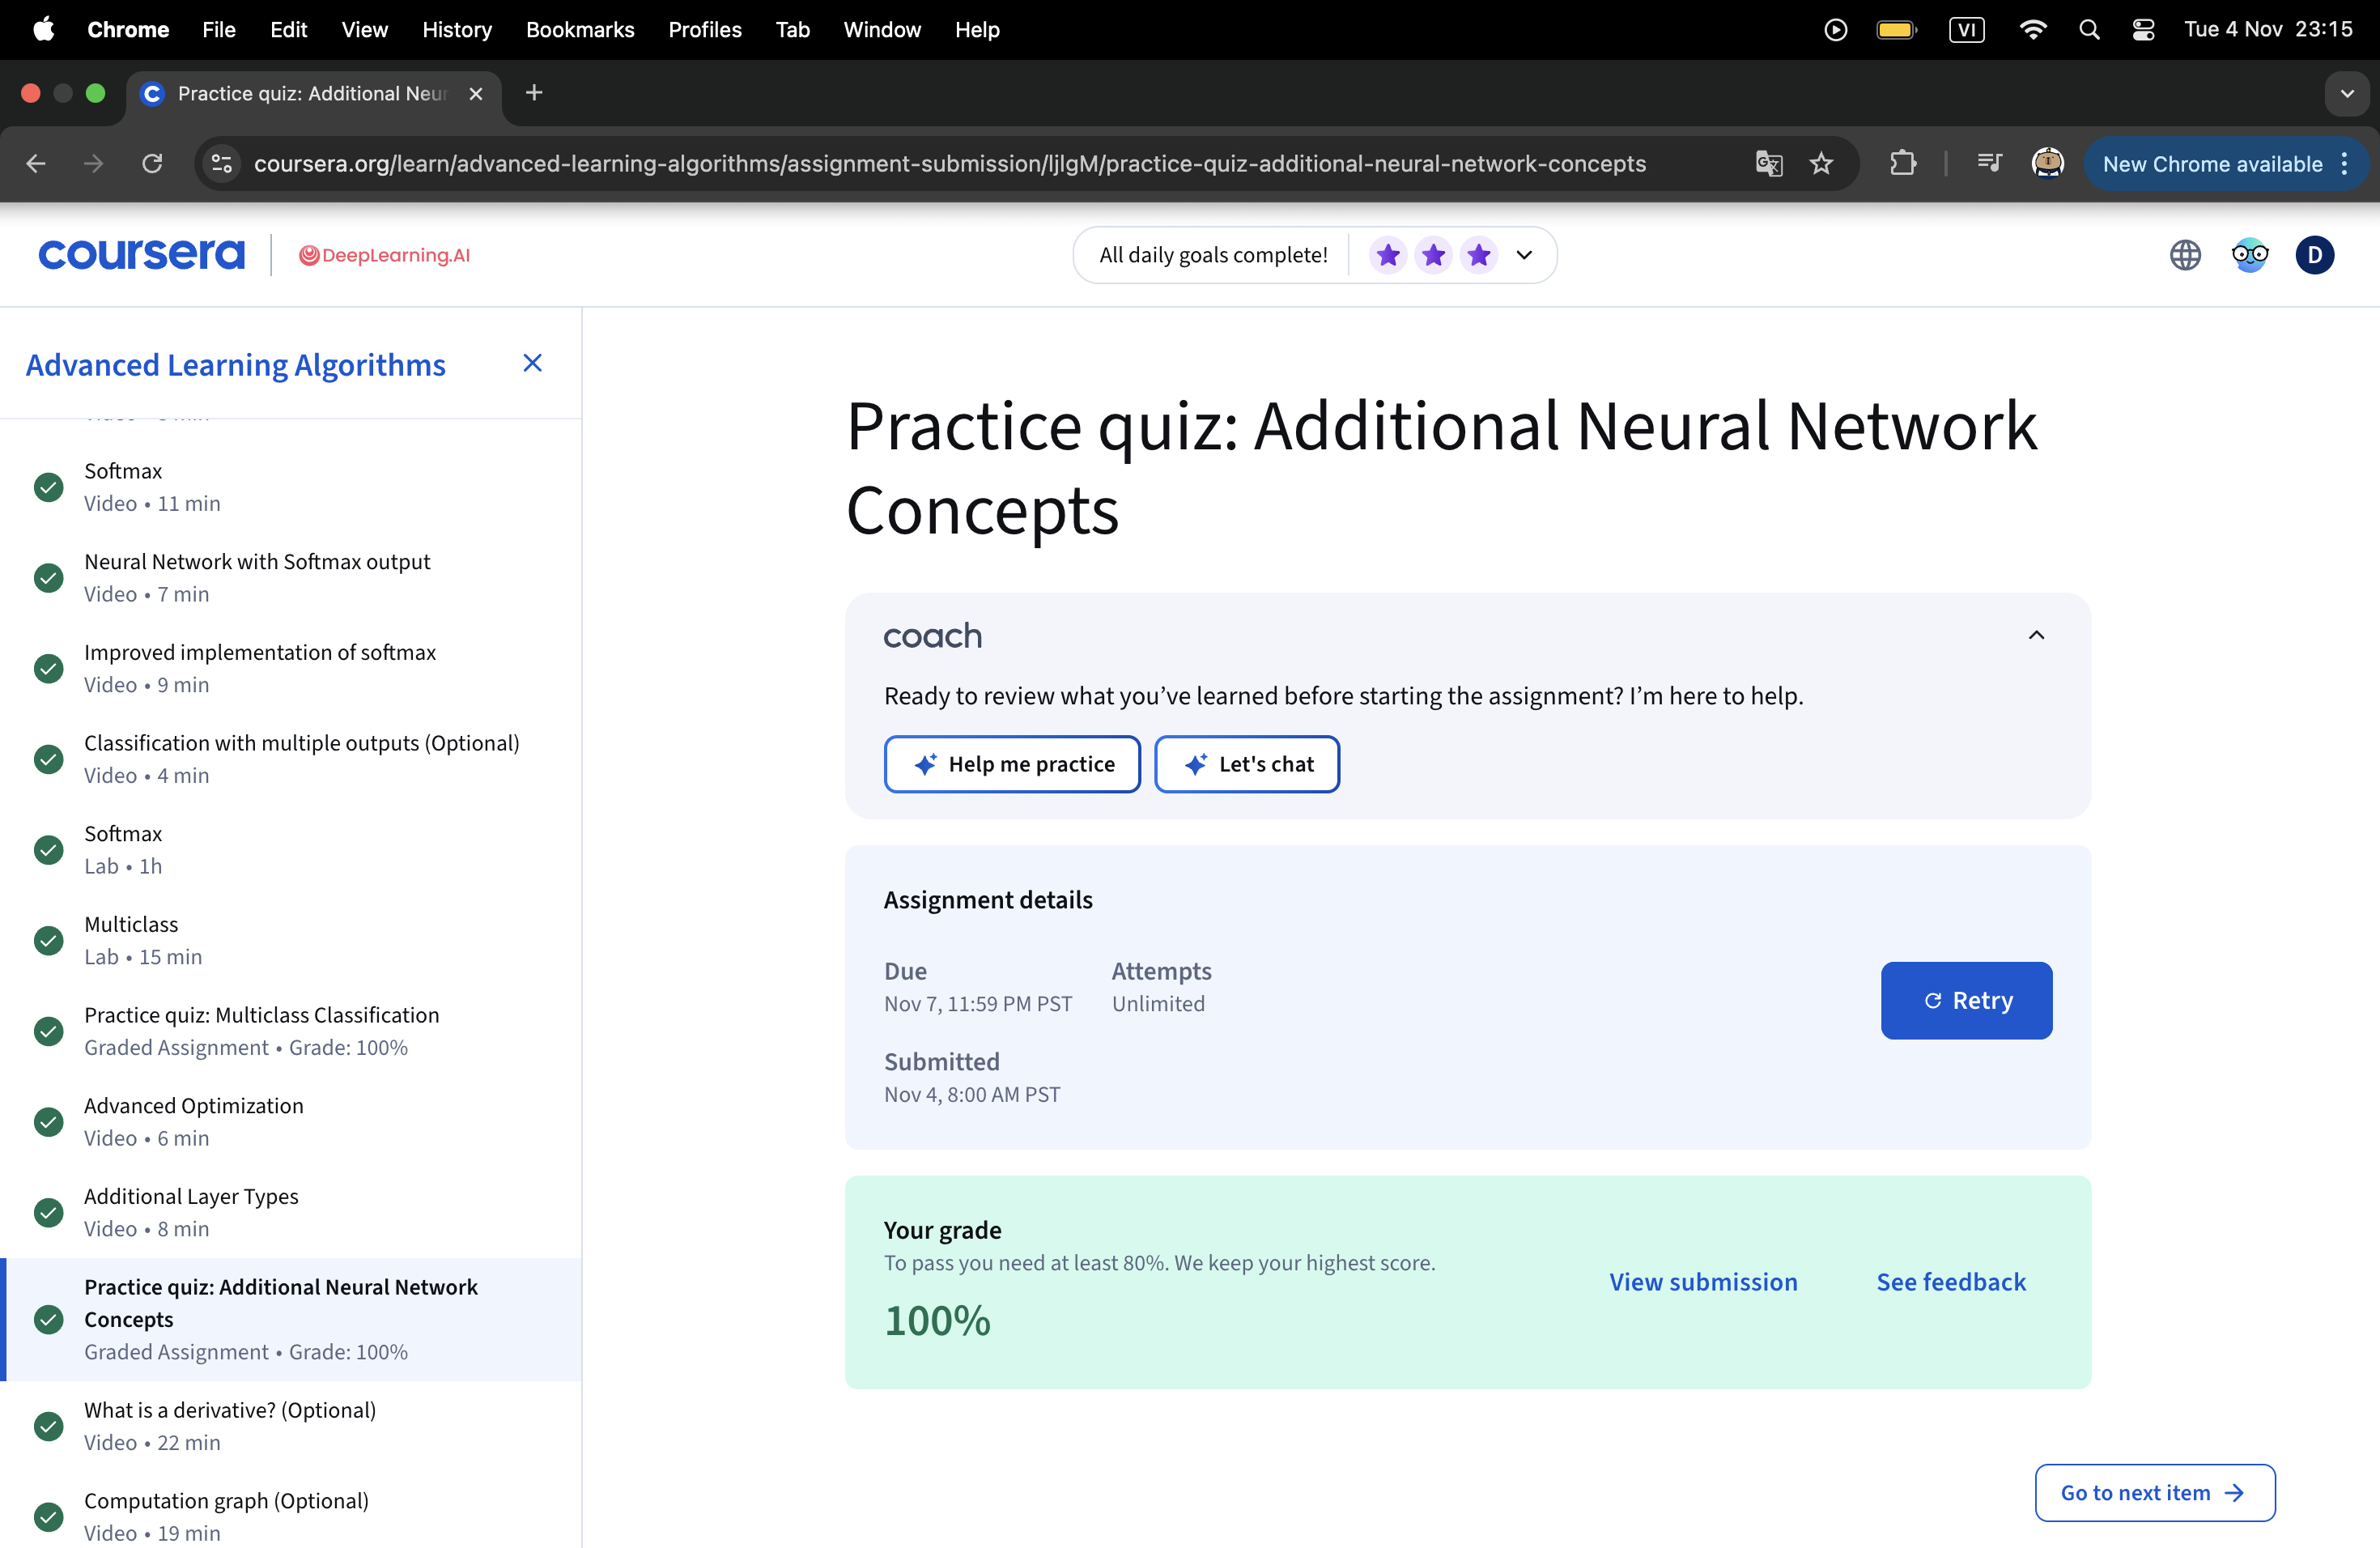
\includegraphics[scale=0.27]{Image/c2_w2_q4.png}
    \caption{Completed Graded Assignment 4 (Additional Neural Network Concepts)}
\end{figure}

\begin{figure}[H]
    \centering
    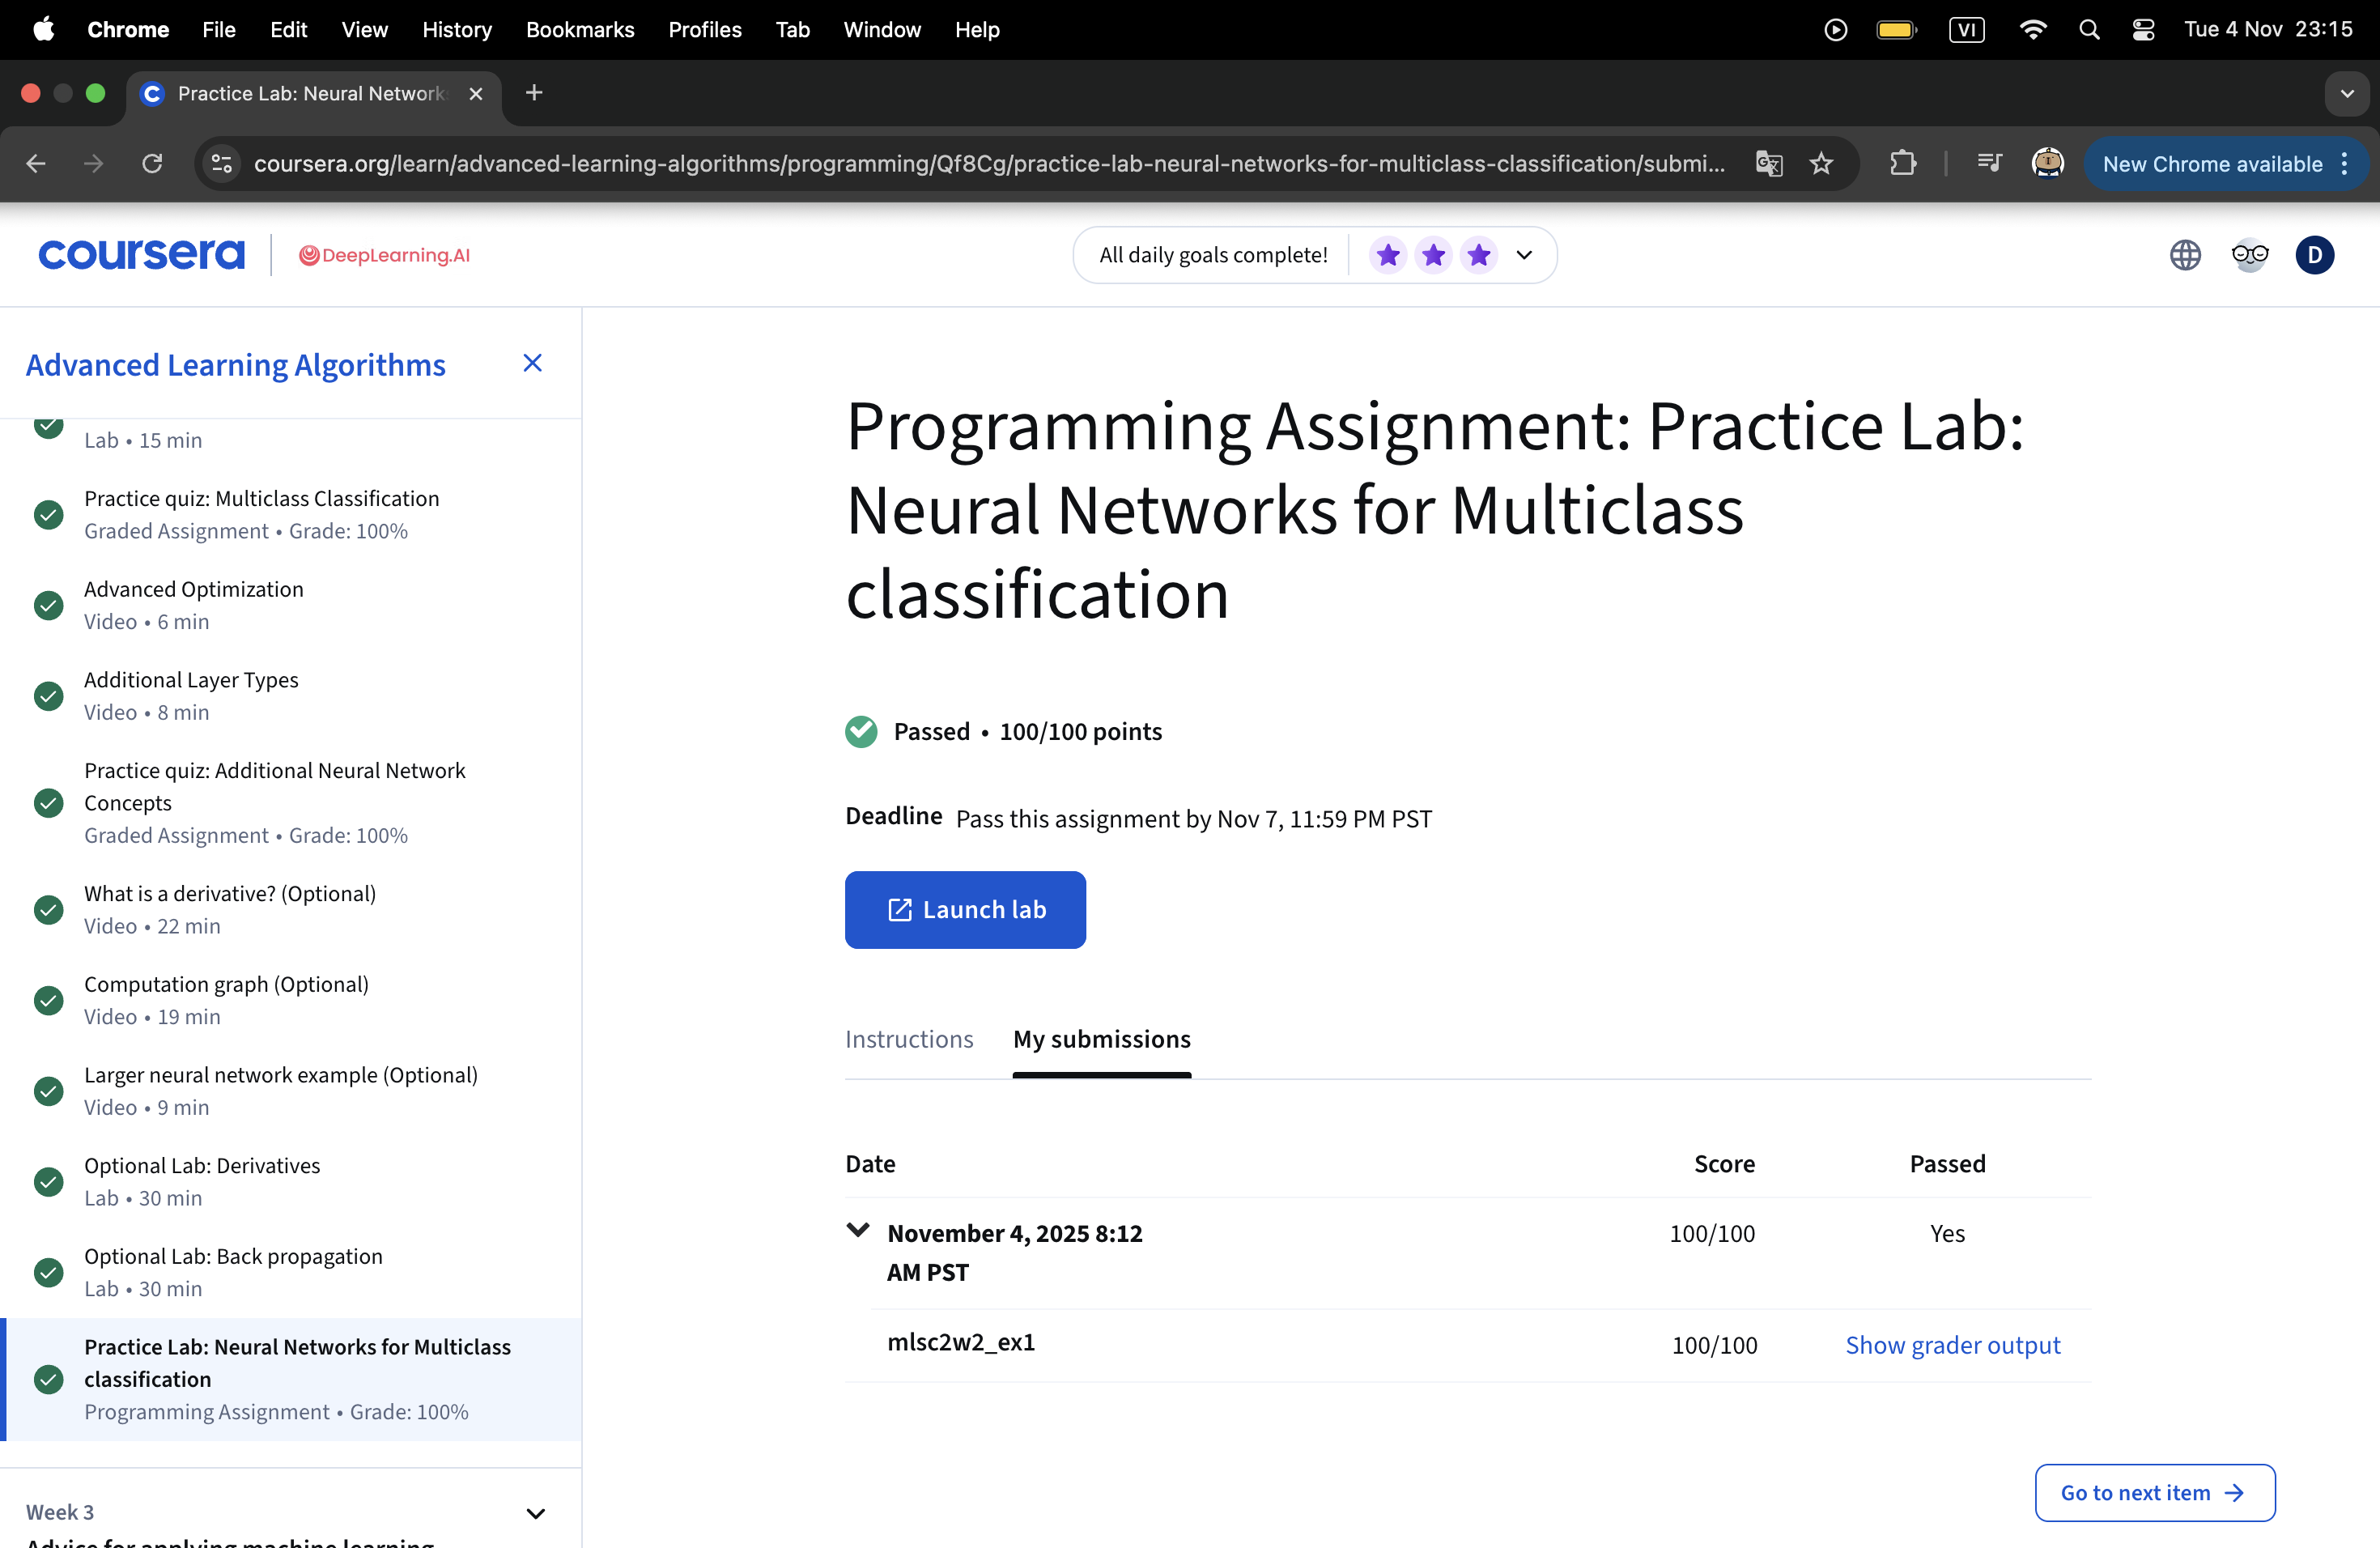
\includegraphics[scale=0.27]{Image/c2_w2_q5.png}
    \caption{Completed Programming Assignment (Neural Networks for Multiclass classification)}
\end{figure}

%----------------------------------------
\subsection{Week 3: Advice for Applying Machine Learning}
%----------------------------------------

\subsubsection{Key Insights and Learnings}

Often considered the most valuable part of the specialization, this module provided a strategic framework for diagnosing and improving model performance.

\begin{itemize}
    \item \textbf{Model Diagnostics (Bias vs. Variance):}
    \begin{itemize}
        \item Utilized \textbf{Learning Curves} to visualize training and cross-validation errors.
        \item \textbf{High Bias (Underfitting):} Addressed by increasing model complexity (adding layers/neurons) or reducing regularization.
        \item \textbf{High Variance (Overfitting):} Addressed by collecting more data or adding regularization/dropout.
    \end{itemize}
    
    \item \textbf{Error Metrics for Skewed Datasets:} Learned that accuracy is misleading for imbalanced classes (e.g., rare disease detection). Adopted \textbf{Precision, Recall}, and the \textbf{F1-Score} as robust evaluation metrics.
    
    \item \textbf{Iterative Loop of ML Development:} Embraced the cycle of \texttt{Idea -> Code -> Experiment}. The systematic split of data into \textbf{Train/Dev (Cross-Validation)/Test} sets is crucial for unbiased tuning.
\end{itemize}

\subsubsection{Learning Evidence}
\begin{figure}[H]
    \centering
    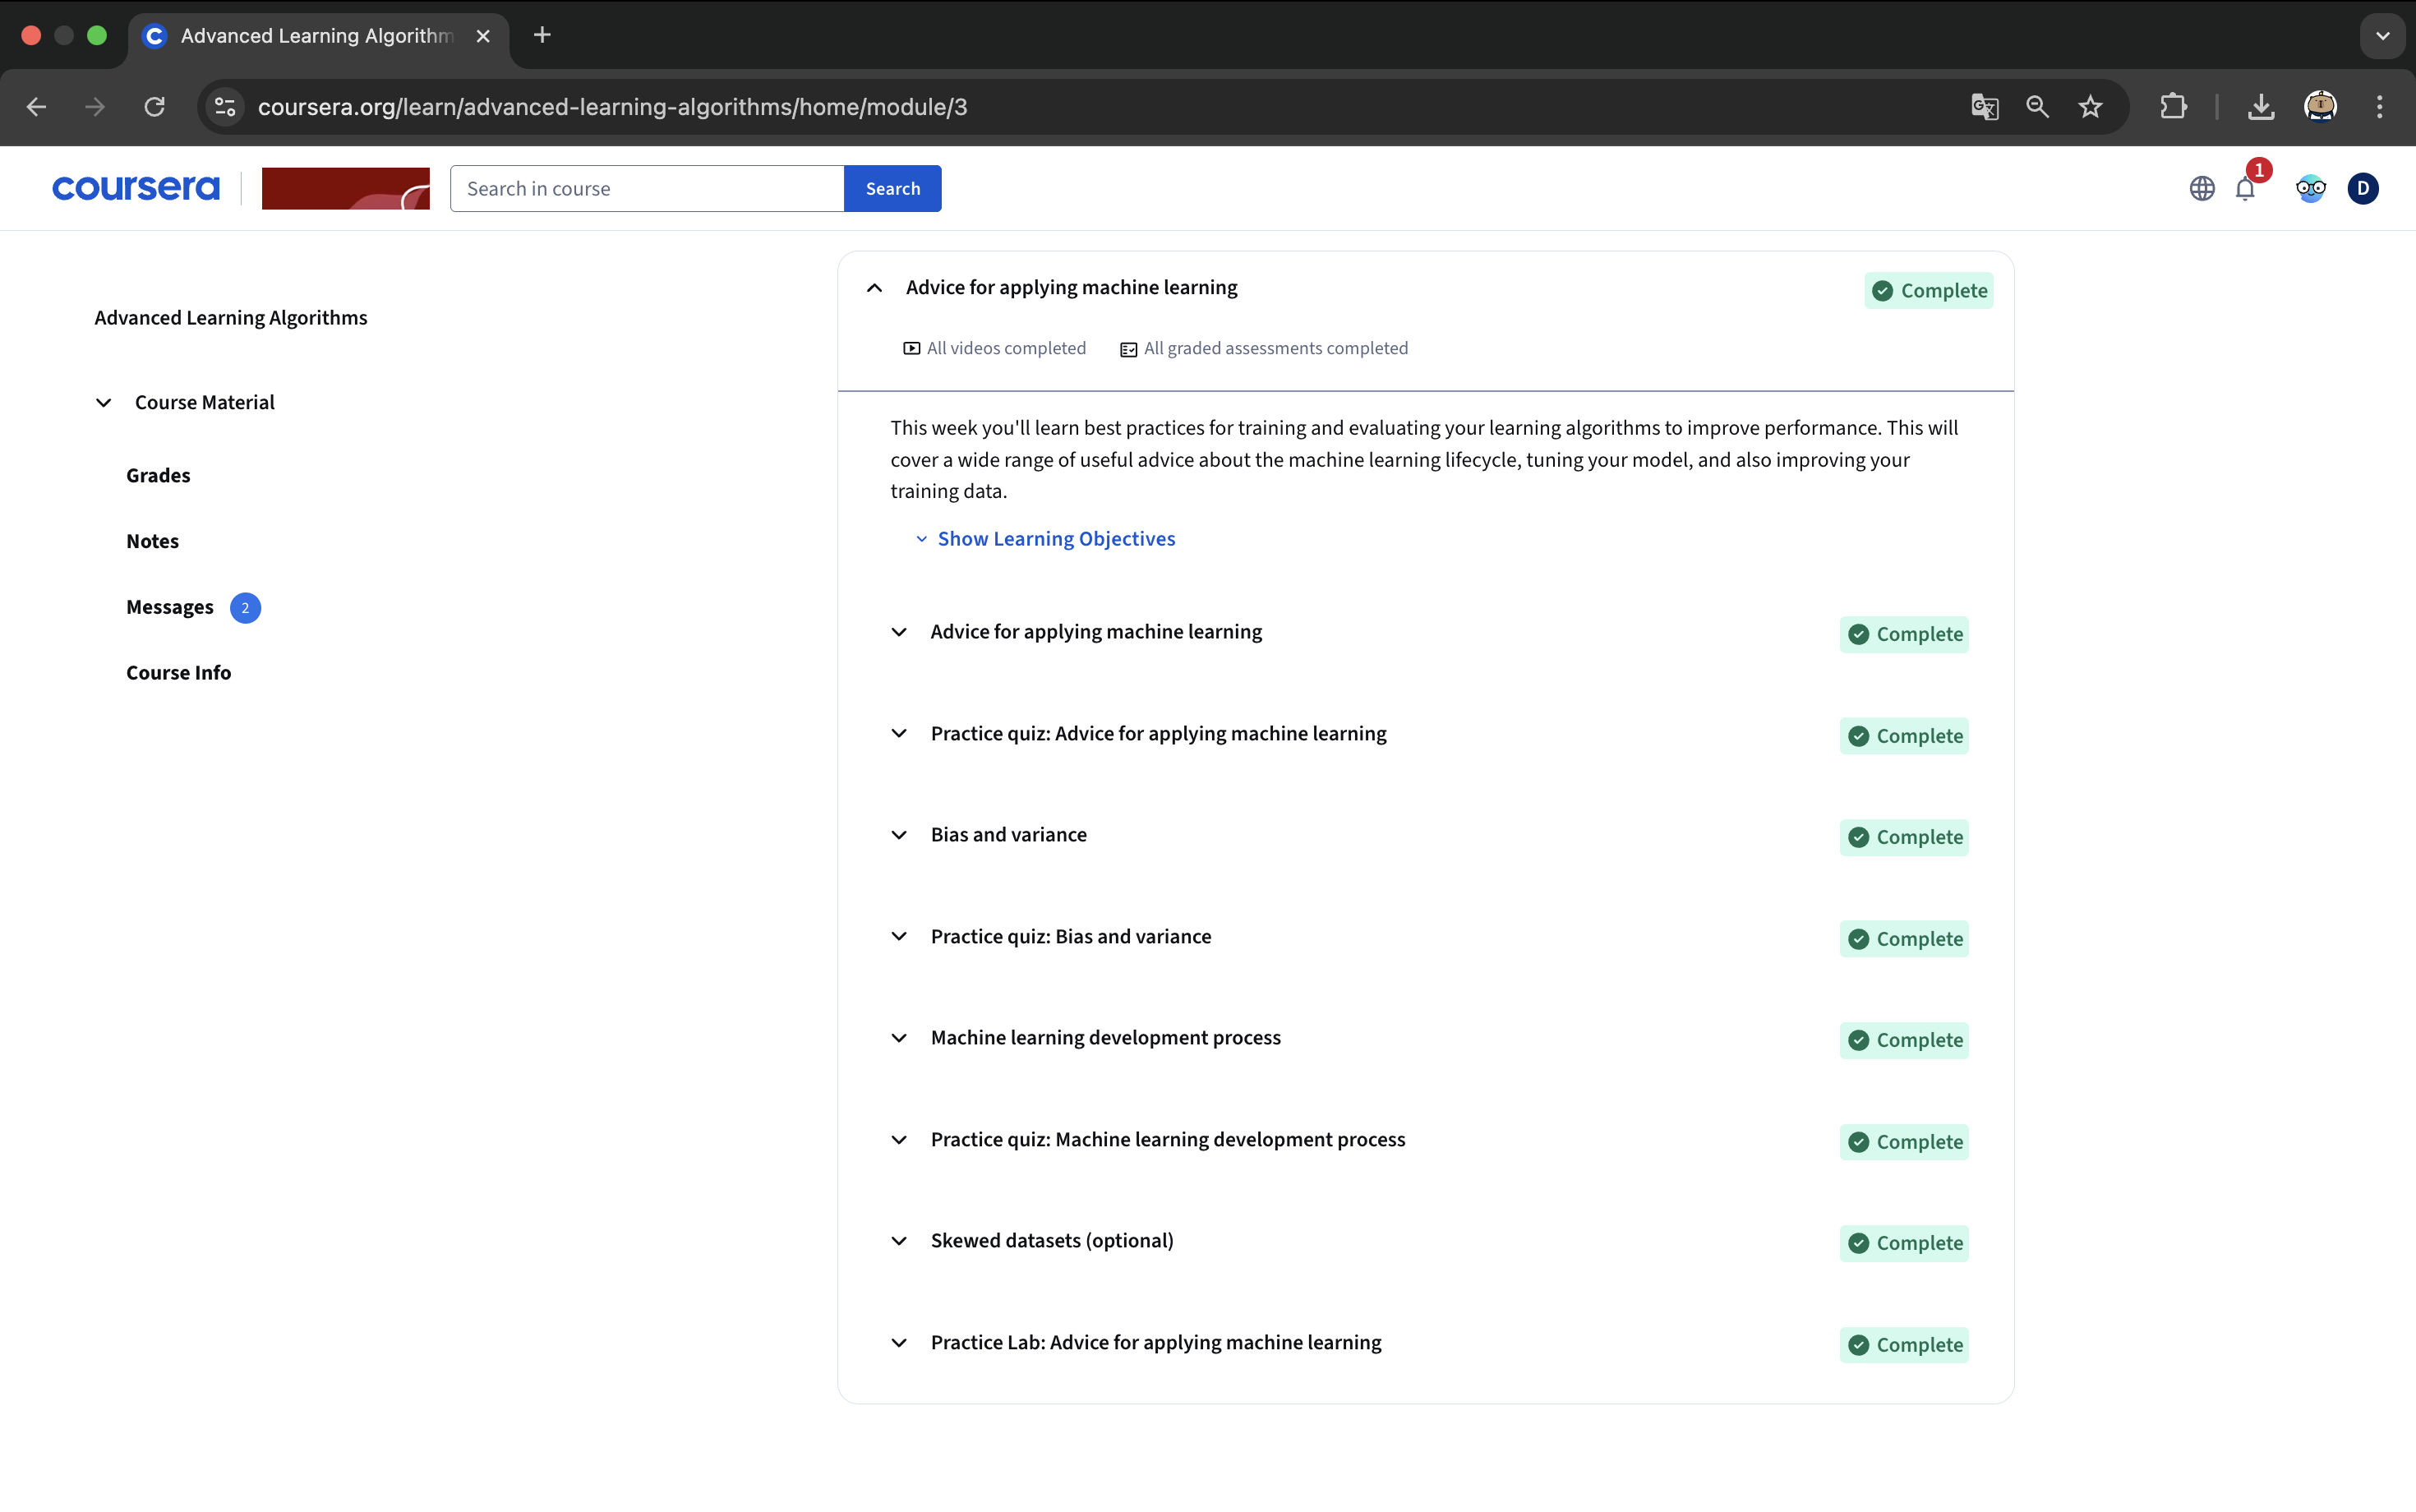
\includegraphics[scale=0.27]{Image/c2_w3.png}
    \caption{Lesson's completed date (07/11/2025)}
\end{figure}

\subsubsection{Graded Assignment Evidence}
\begin{figure}[H]
    \centering
    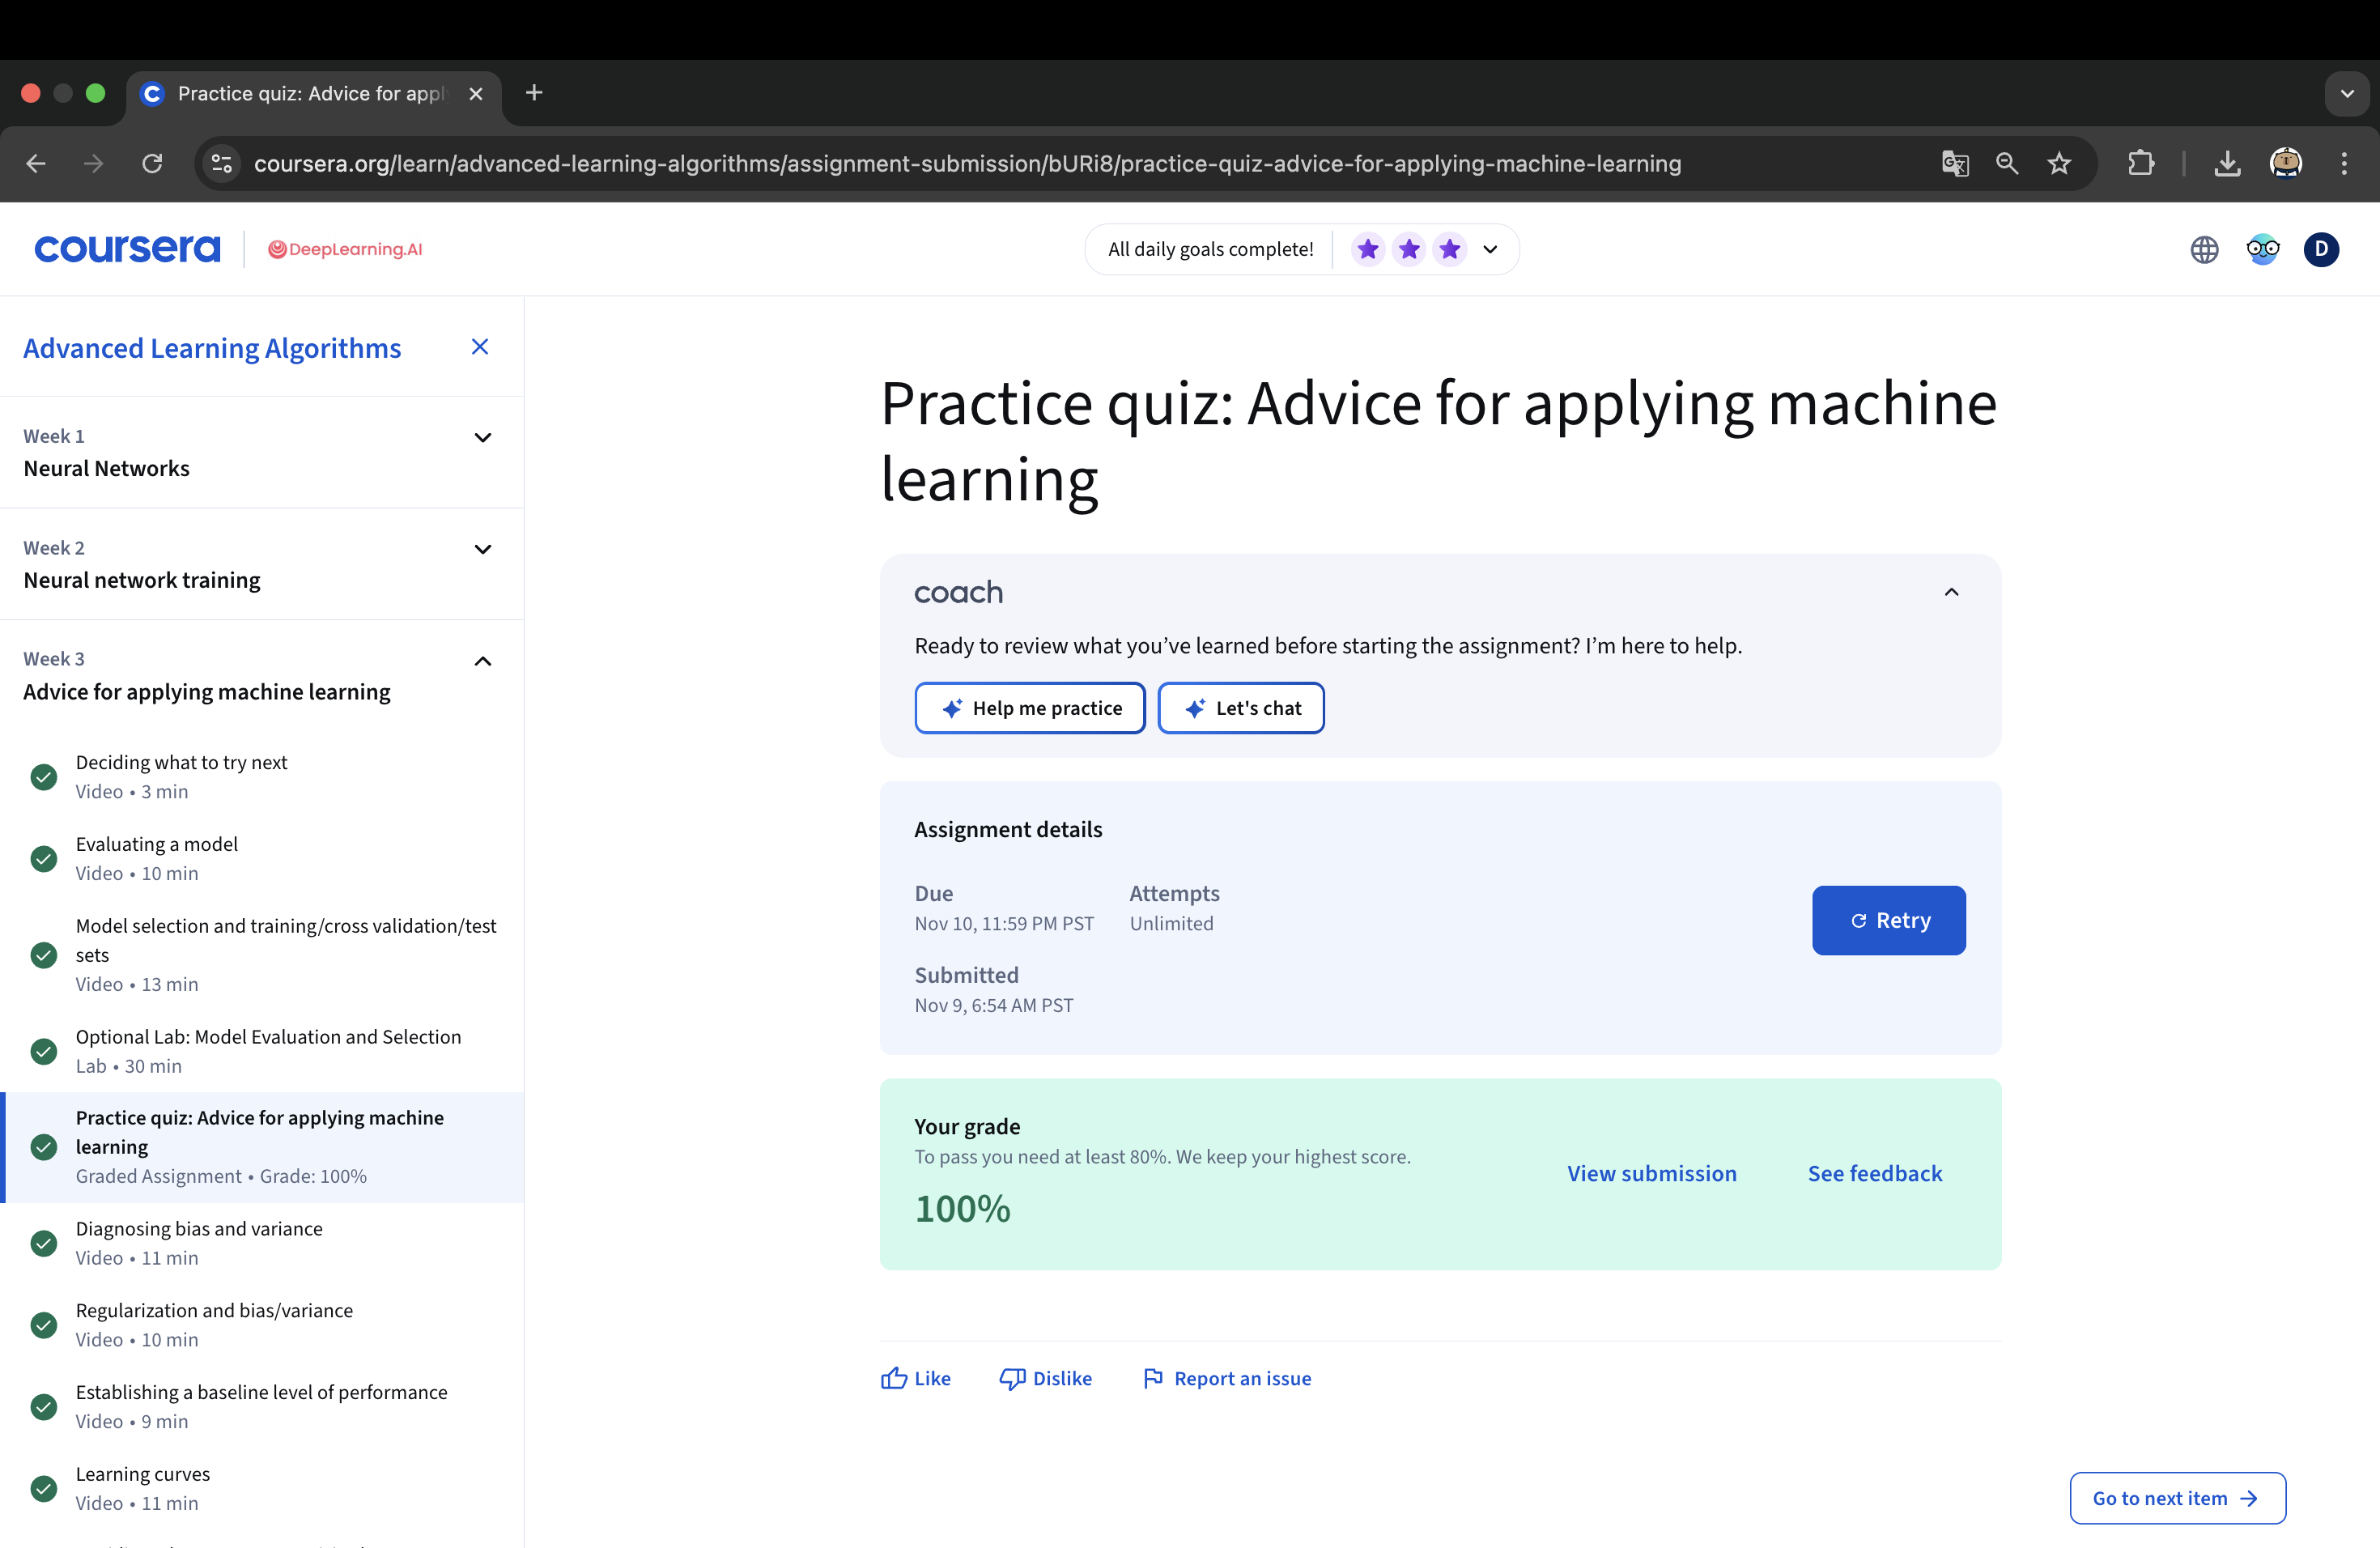
\includegraphics[scale=0.25]{Image/c2_w3_q1.png}
    \caption{Completed Graded Assignment 1 (Advice for applying machine learning)}
\end{figure}

\begin{figure}[H]
    \centering
    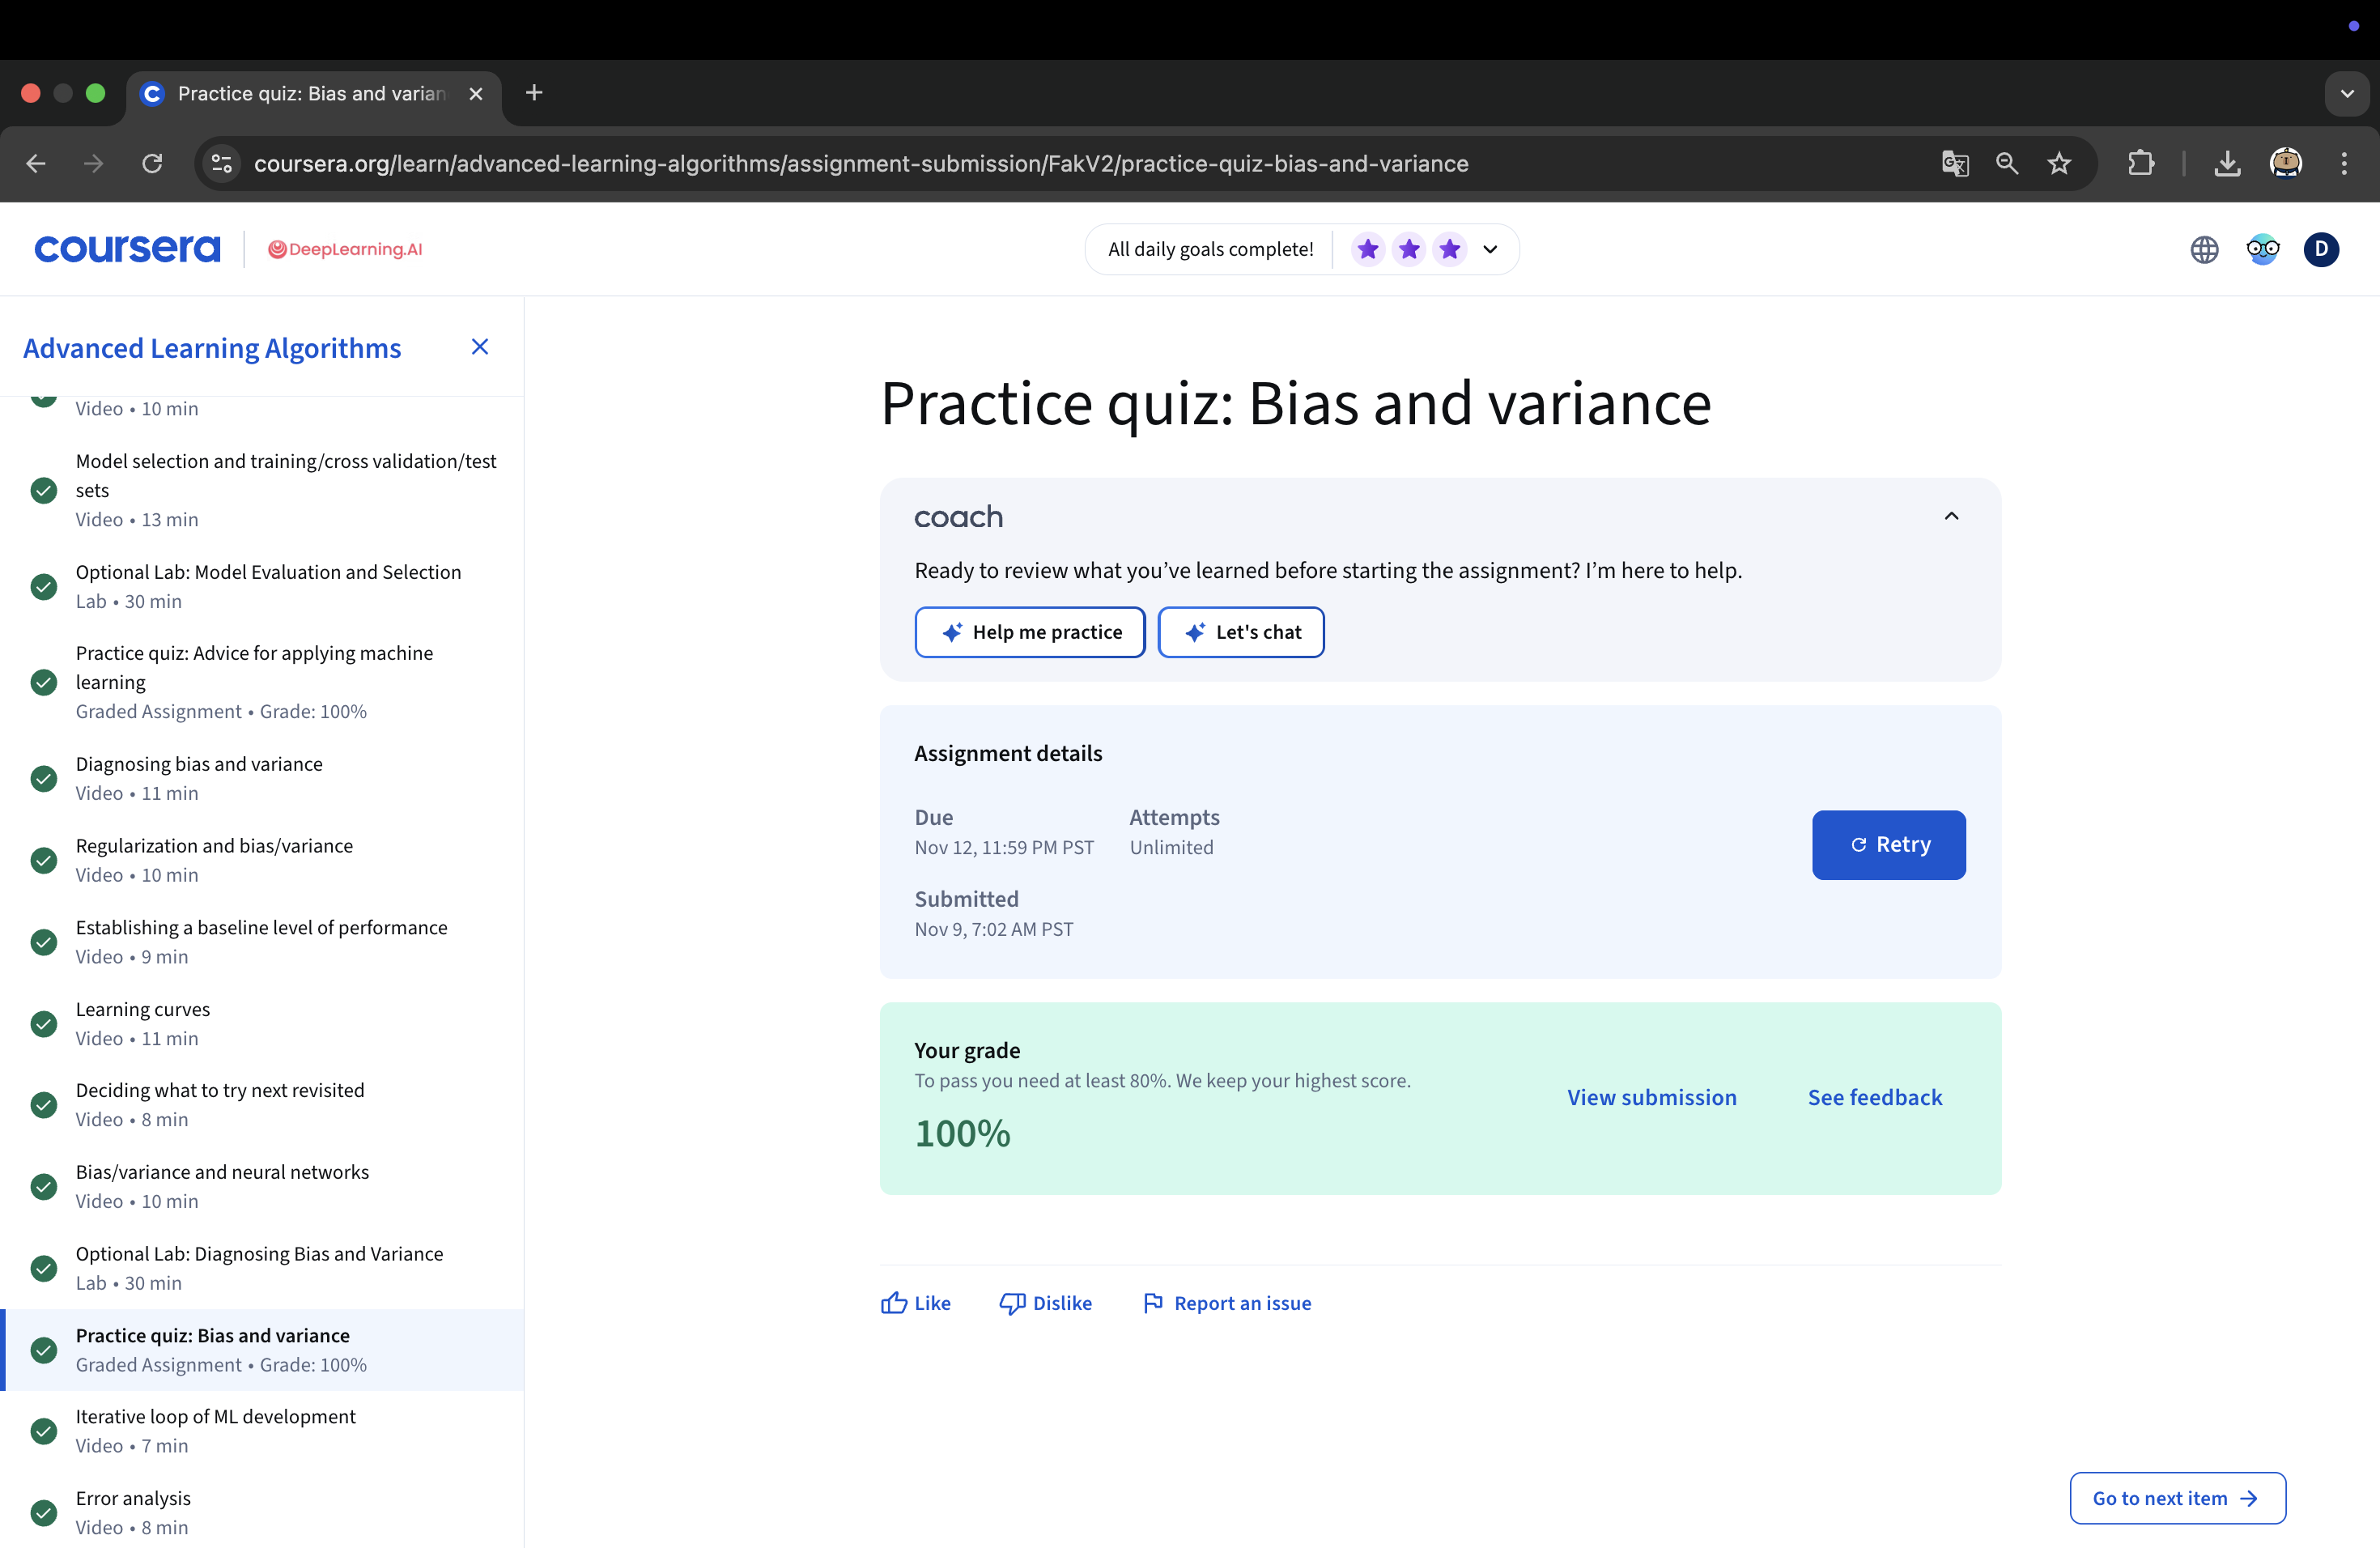
\includegraphics[scale=0.27]{Image/c2_w3_q2.png}
    \caption{Completed Graded Assignment 2 (Bias and variance)}
\end{figure}

\begin{figure}[H]
    \centering
    
\includegraphics[scale=0.27]{Image/c2_w3_q3.png}
    \caption{Completed Graded Assignment 3 (Machine learning development process)}
\end{figure}

\begin{figure}[H]
    \centering
    
\includegraphics[scale=0.27]{Image/c2_w3_q4.png}
    \caption{Completed Programming Assignment (Advice for Applying Machine Learning)}
\end{figure}

%----------------------------------------
\subsection{Week 4: Decision Trees and Ensemble Methods}
%----------------------------------------

\subsubsection{Key Insights and Learnings}

This module introduced robust alternatives to Neural Networks, particularly effective for structured (tabular) data.

\begin{itemize}
    \item \textbf{Decision Trees Mechanics:}
    \begin{itemize}
        \item The learning process involves recursively splitting data to maximize \textbf{Information Gain} (reducing Entropy).
        \item Highly interpretable models where decision paths can be visualized and explained to non-technical stakeholders.
    \end{itemize}
    
    \item \textbf{Ensemble Methods (The Wisdom of Crowds):}
    \begin{itemize}
        \item \textbf{Random Forests (Bagging):} Builds multiple trees on random subsets of data (sampling with replacement). It averages predictions to reduce \textbf{variance} and prevent overfitting.
        \item \textbf{XGBoost (Boosting):} A state-of-the-art algorithm that trains trees sequentially. Each new tree focuses on correcting the residual errors of the previous ones. It is currently the industry standard for tabular data competitions (e.g., Kaggle).
    \end{itemize}
\end{itemize}

\subsubsection{Learning Evidence}
\begin{figure}[H]
    \centering
    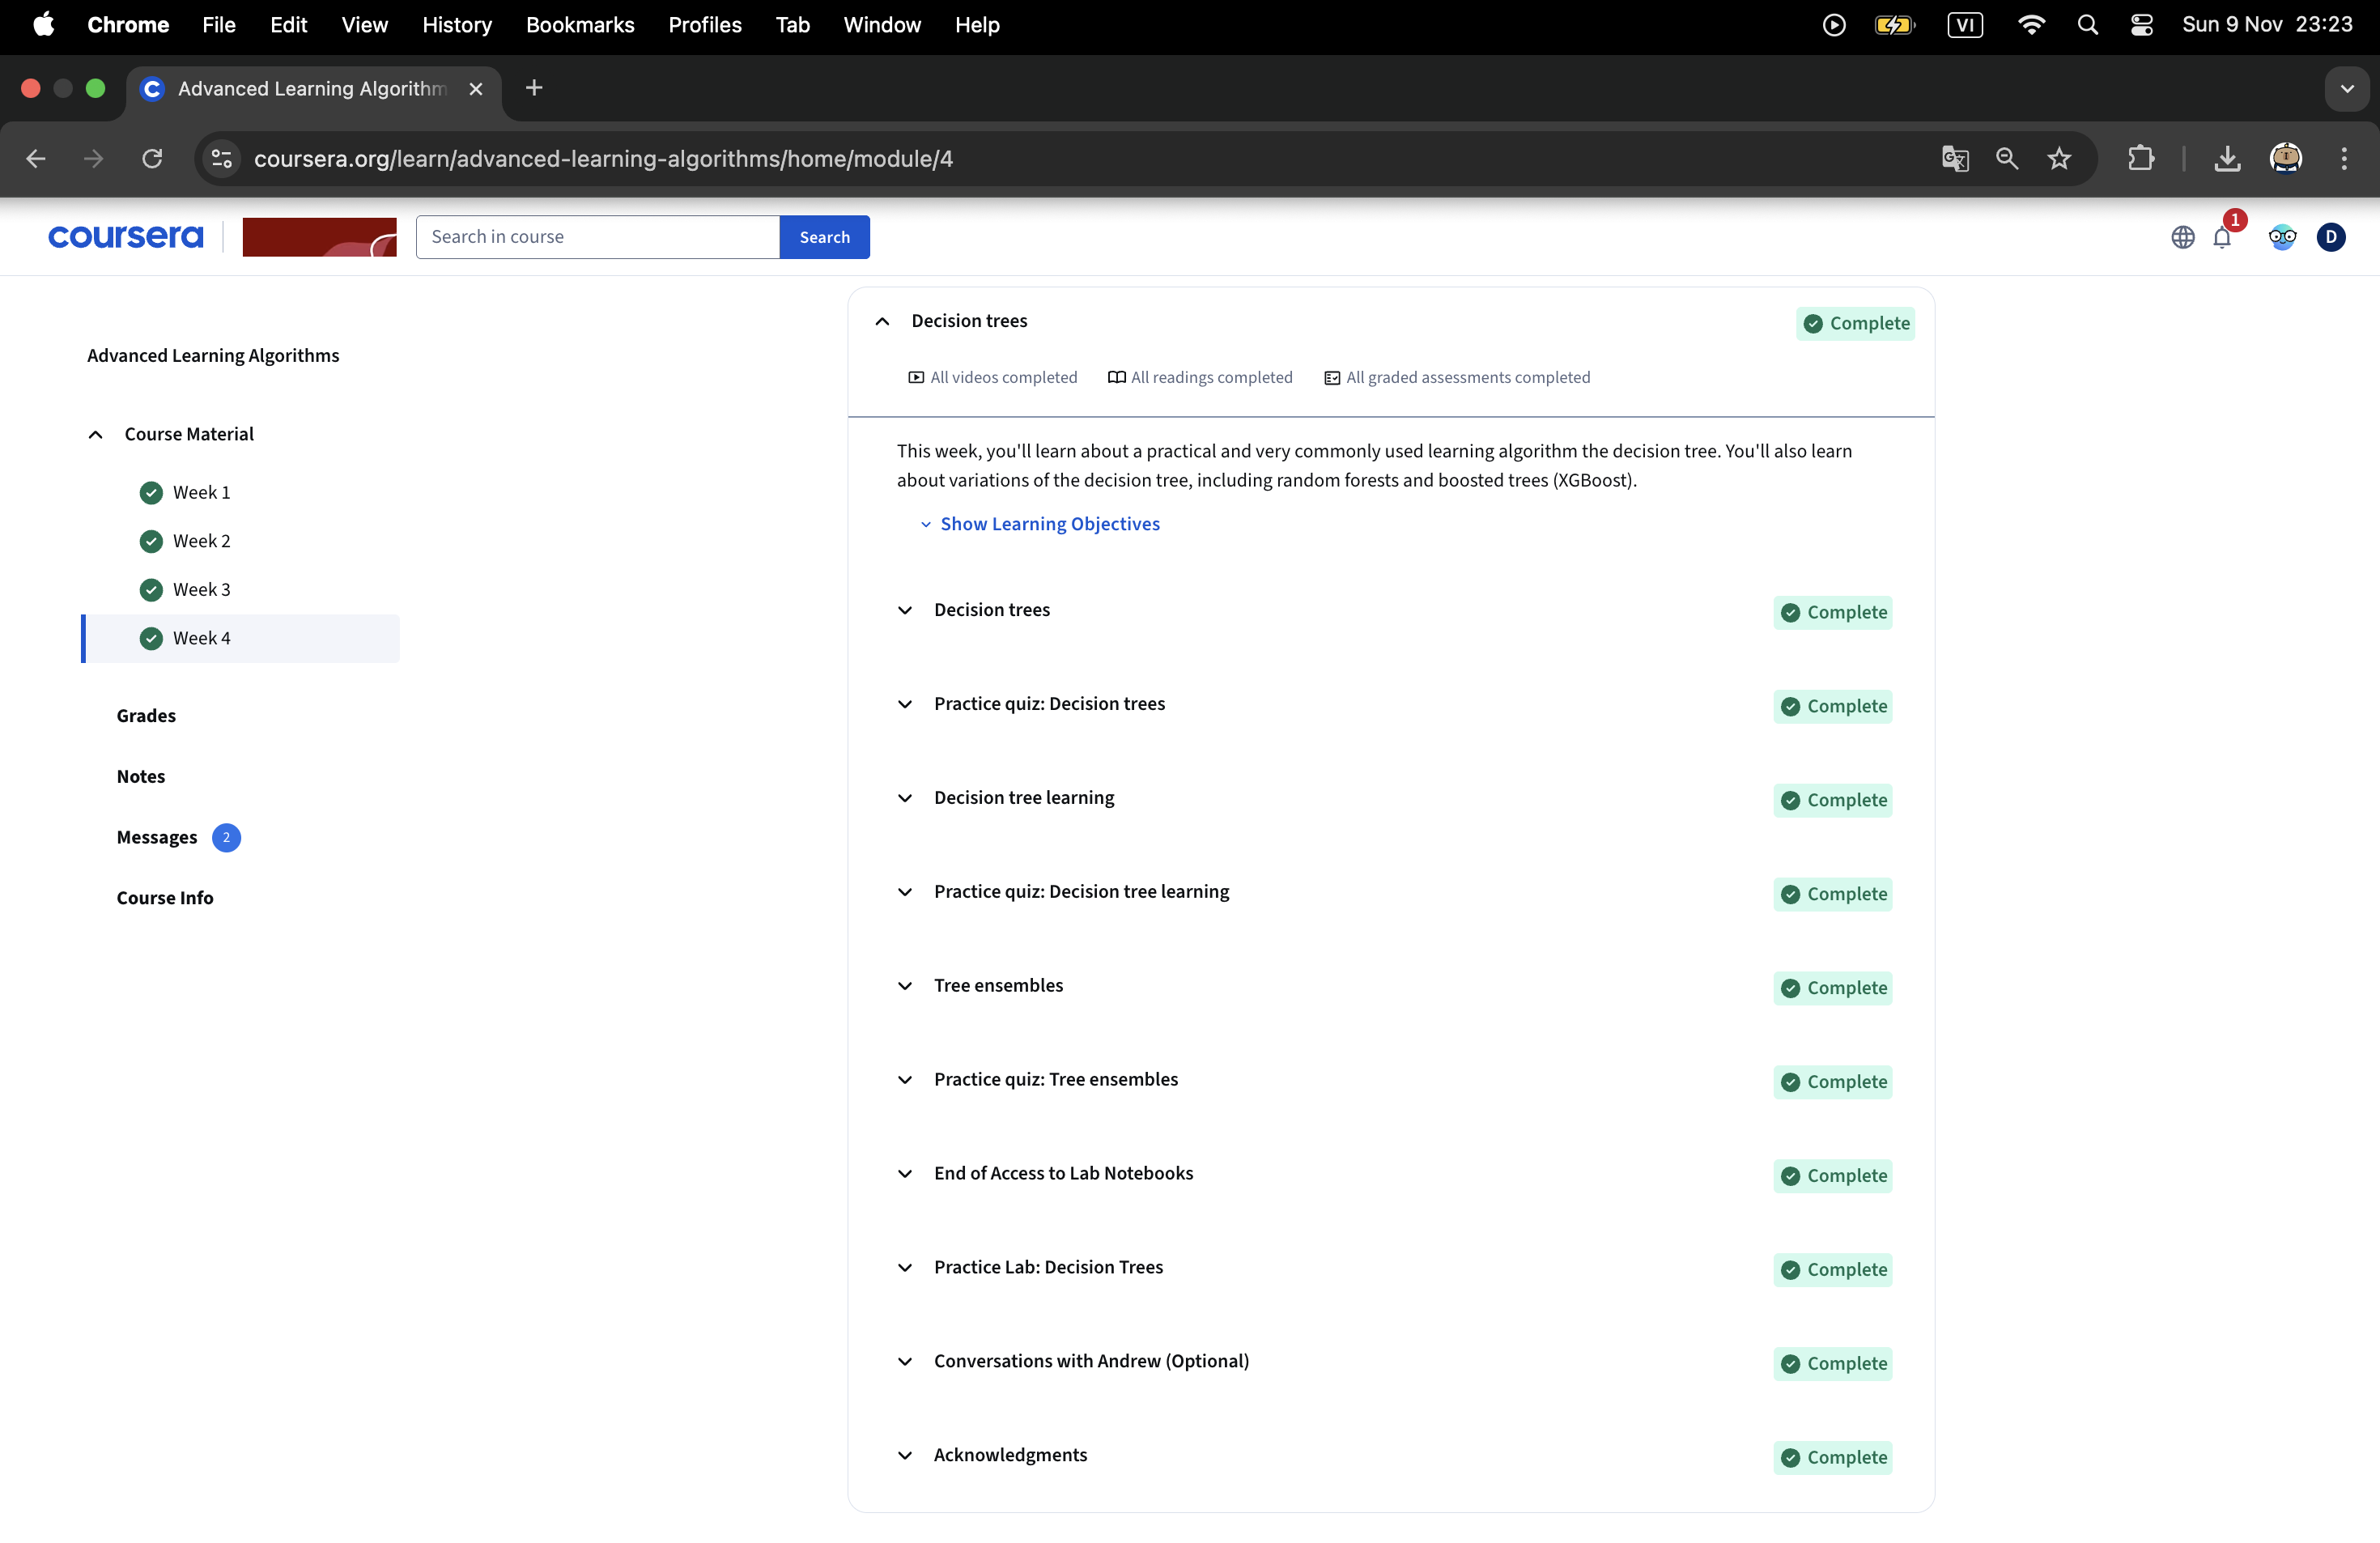
\includegraphics[scale=0.25]{Image/c2_w4.png}
    \caption{Lesson's completed date (09/11/2025)}
\end{figure}

\subsubsection{Graded Assignment Evidence}
\begin{figure}[H]
    \centering
    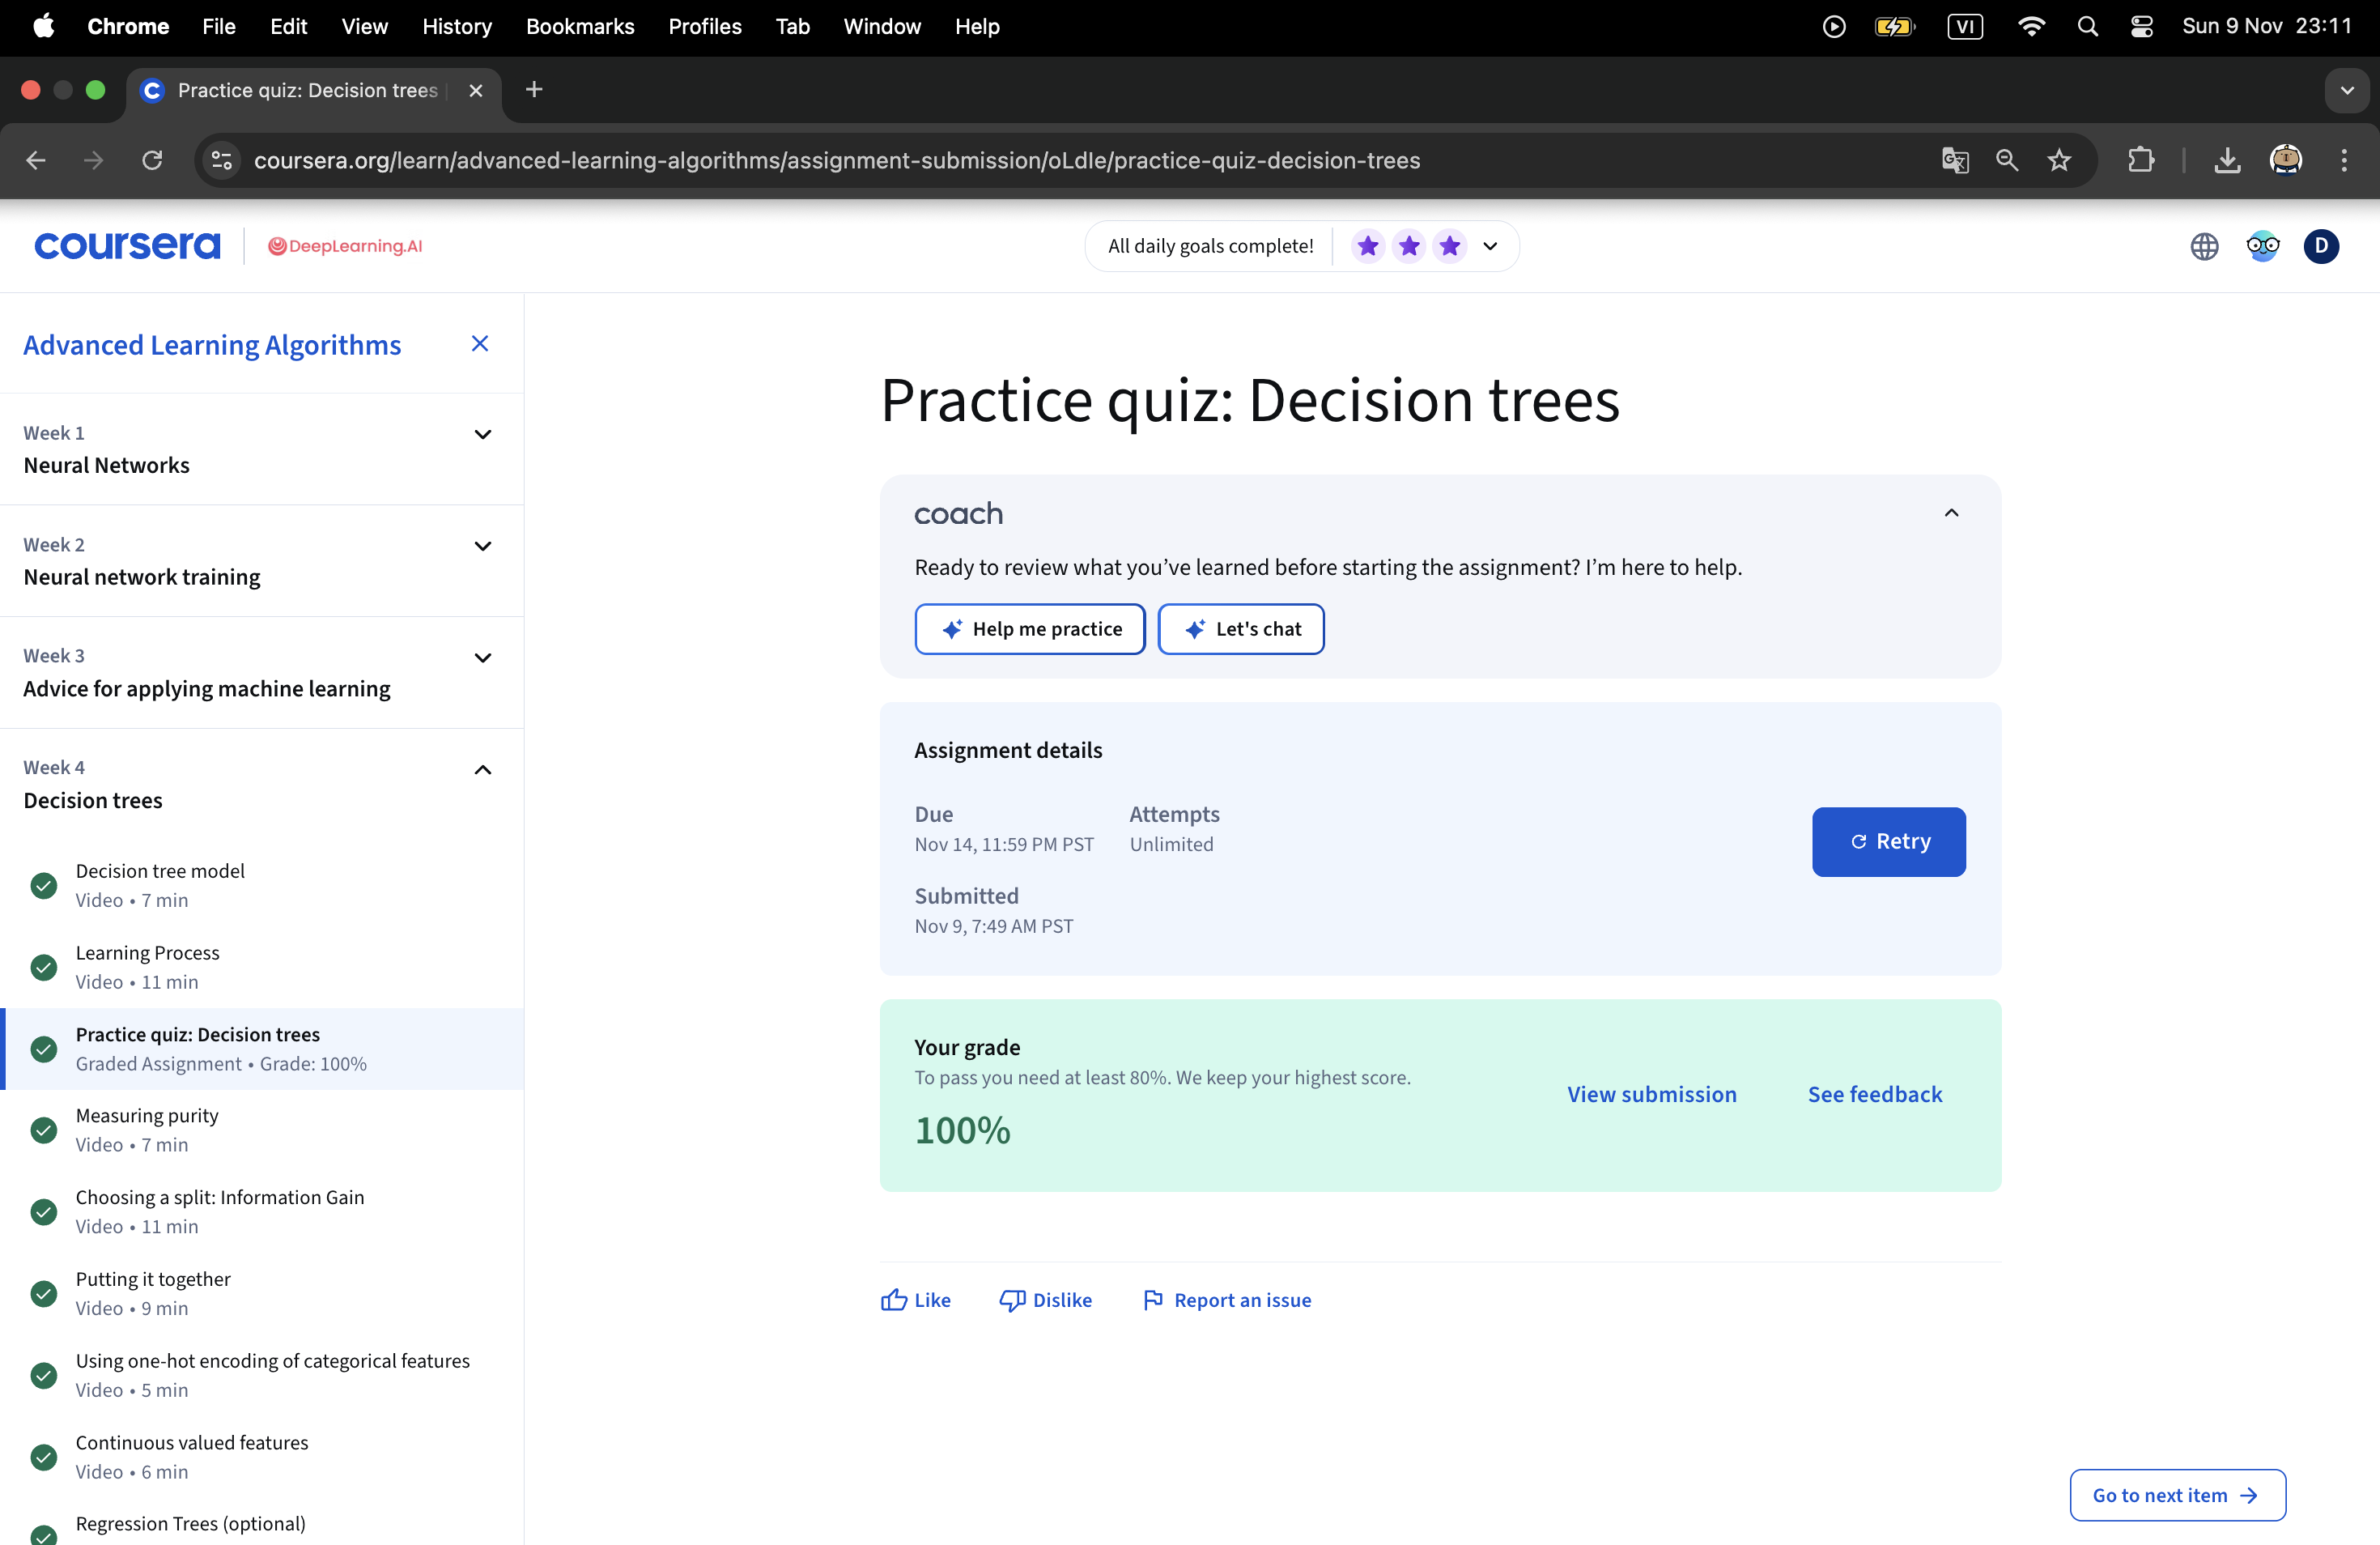
\includegraphics[scale=0.25]{Image/c2_w4_q1.png}
    \caption{Completed Graded Assignment 1 (Decision trees)}
\end{figure}

\begin{figure}[H]
    \centering
    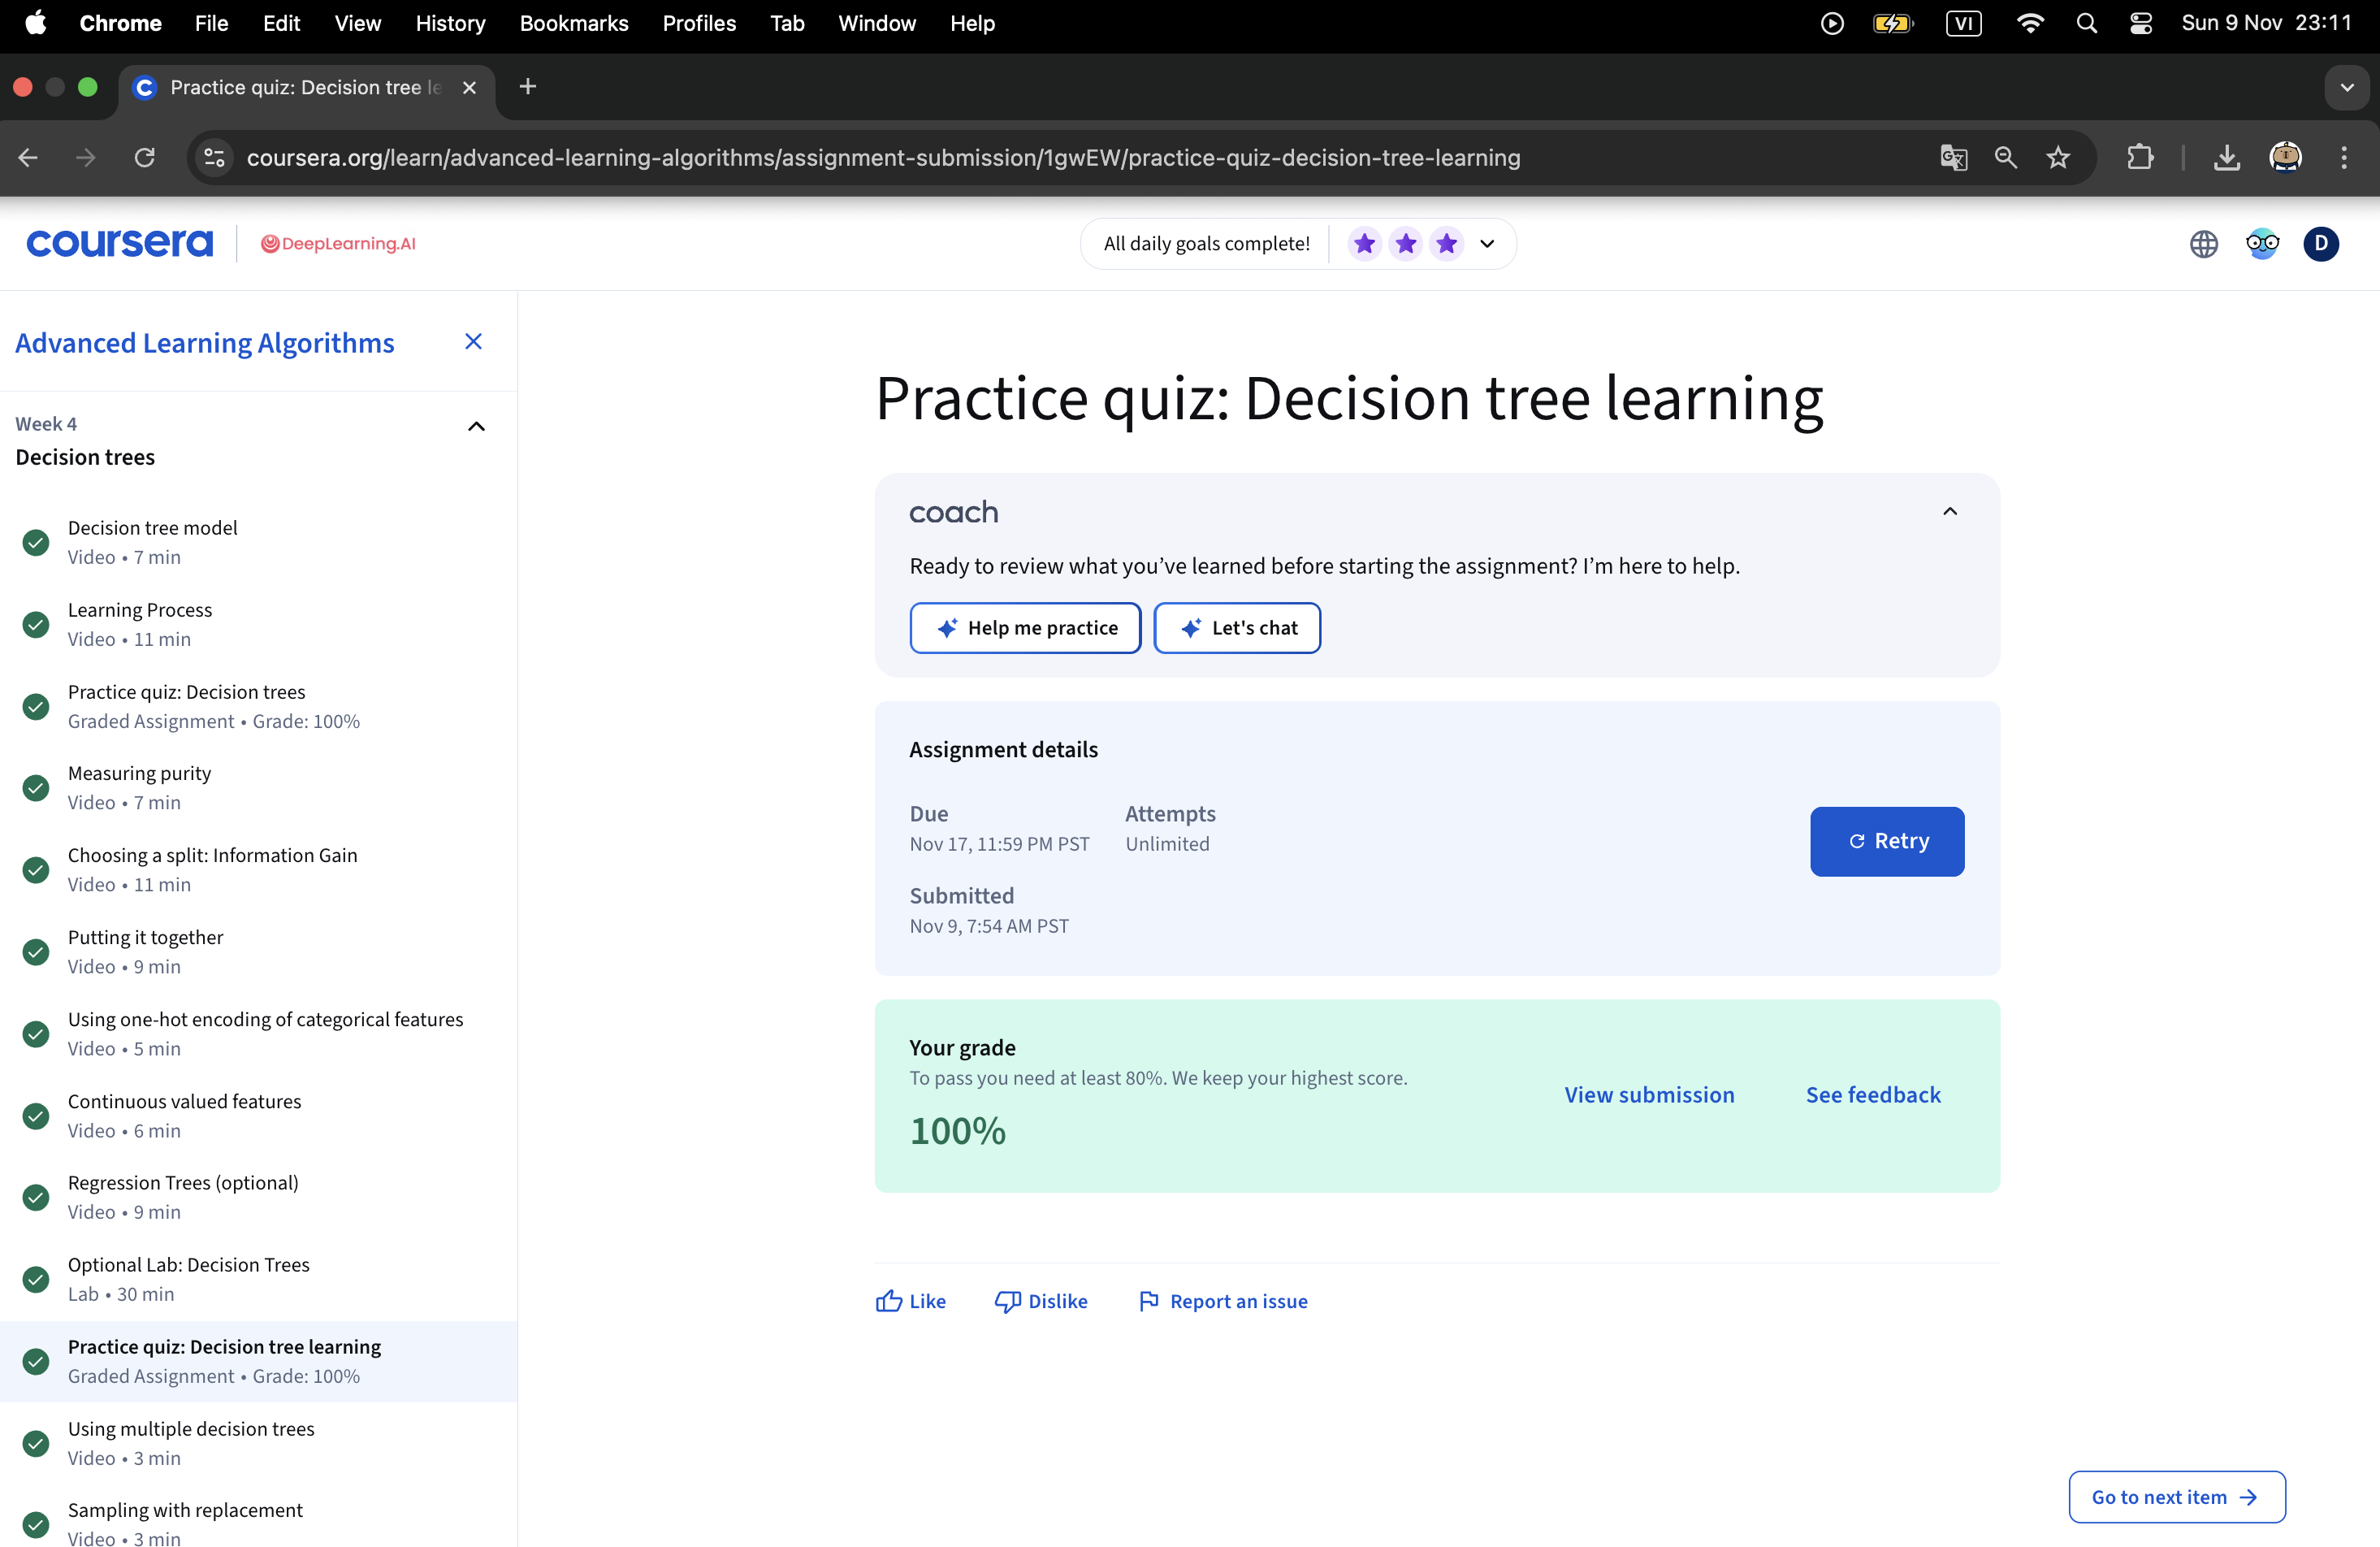
\includegraphics[scale=0.25]{Image/c2_w4_q2.png}
    \caption{Completed Graded Assignment 2 (Decision tree learning)}
\end{figure}

\begin{figure}[H]
    \centering
    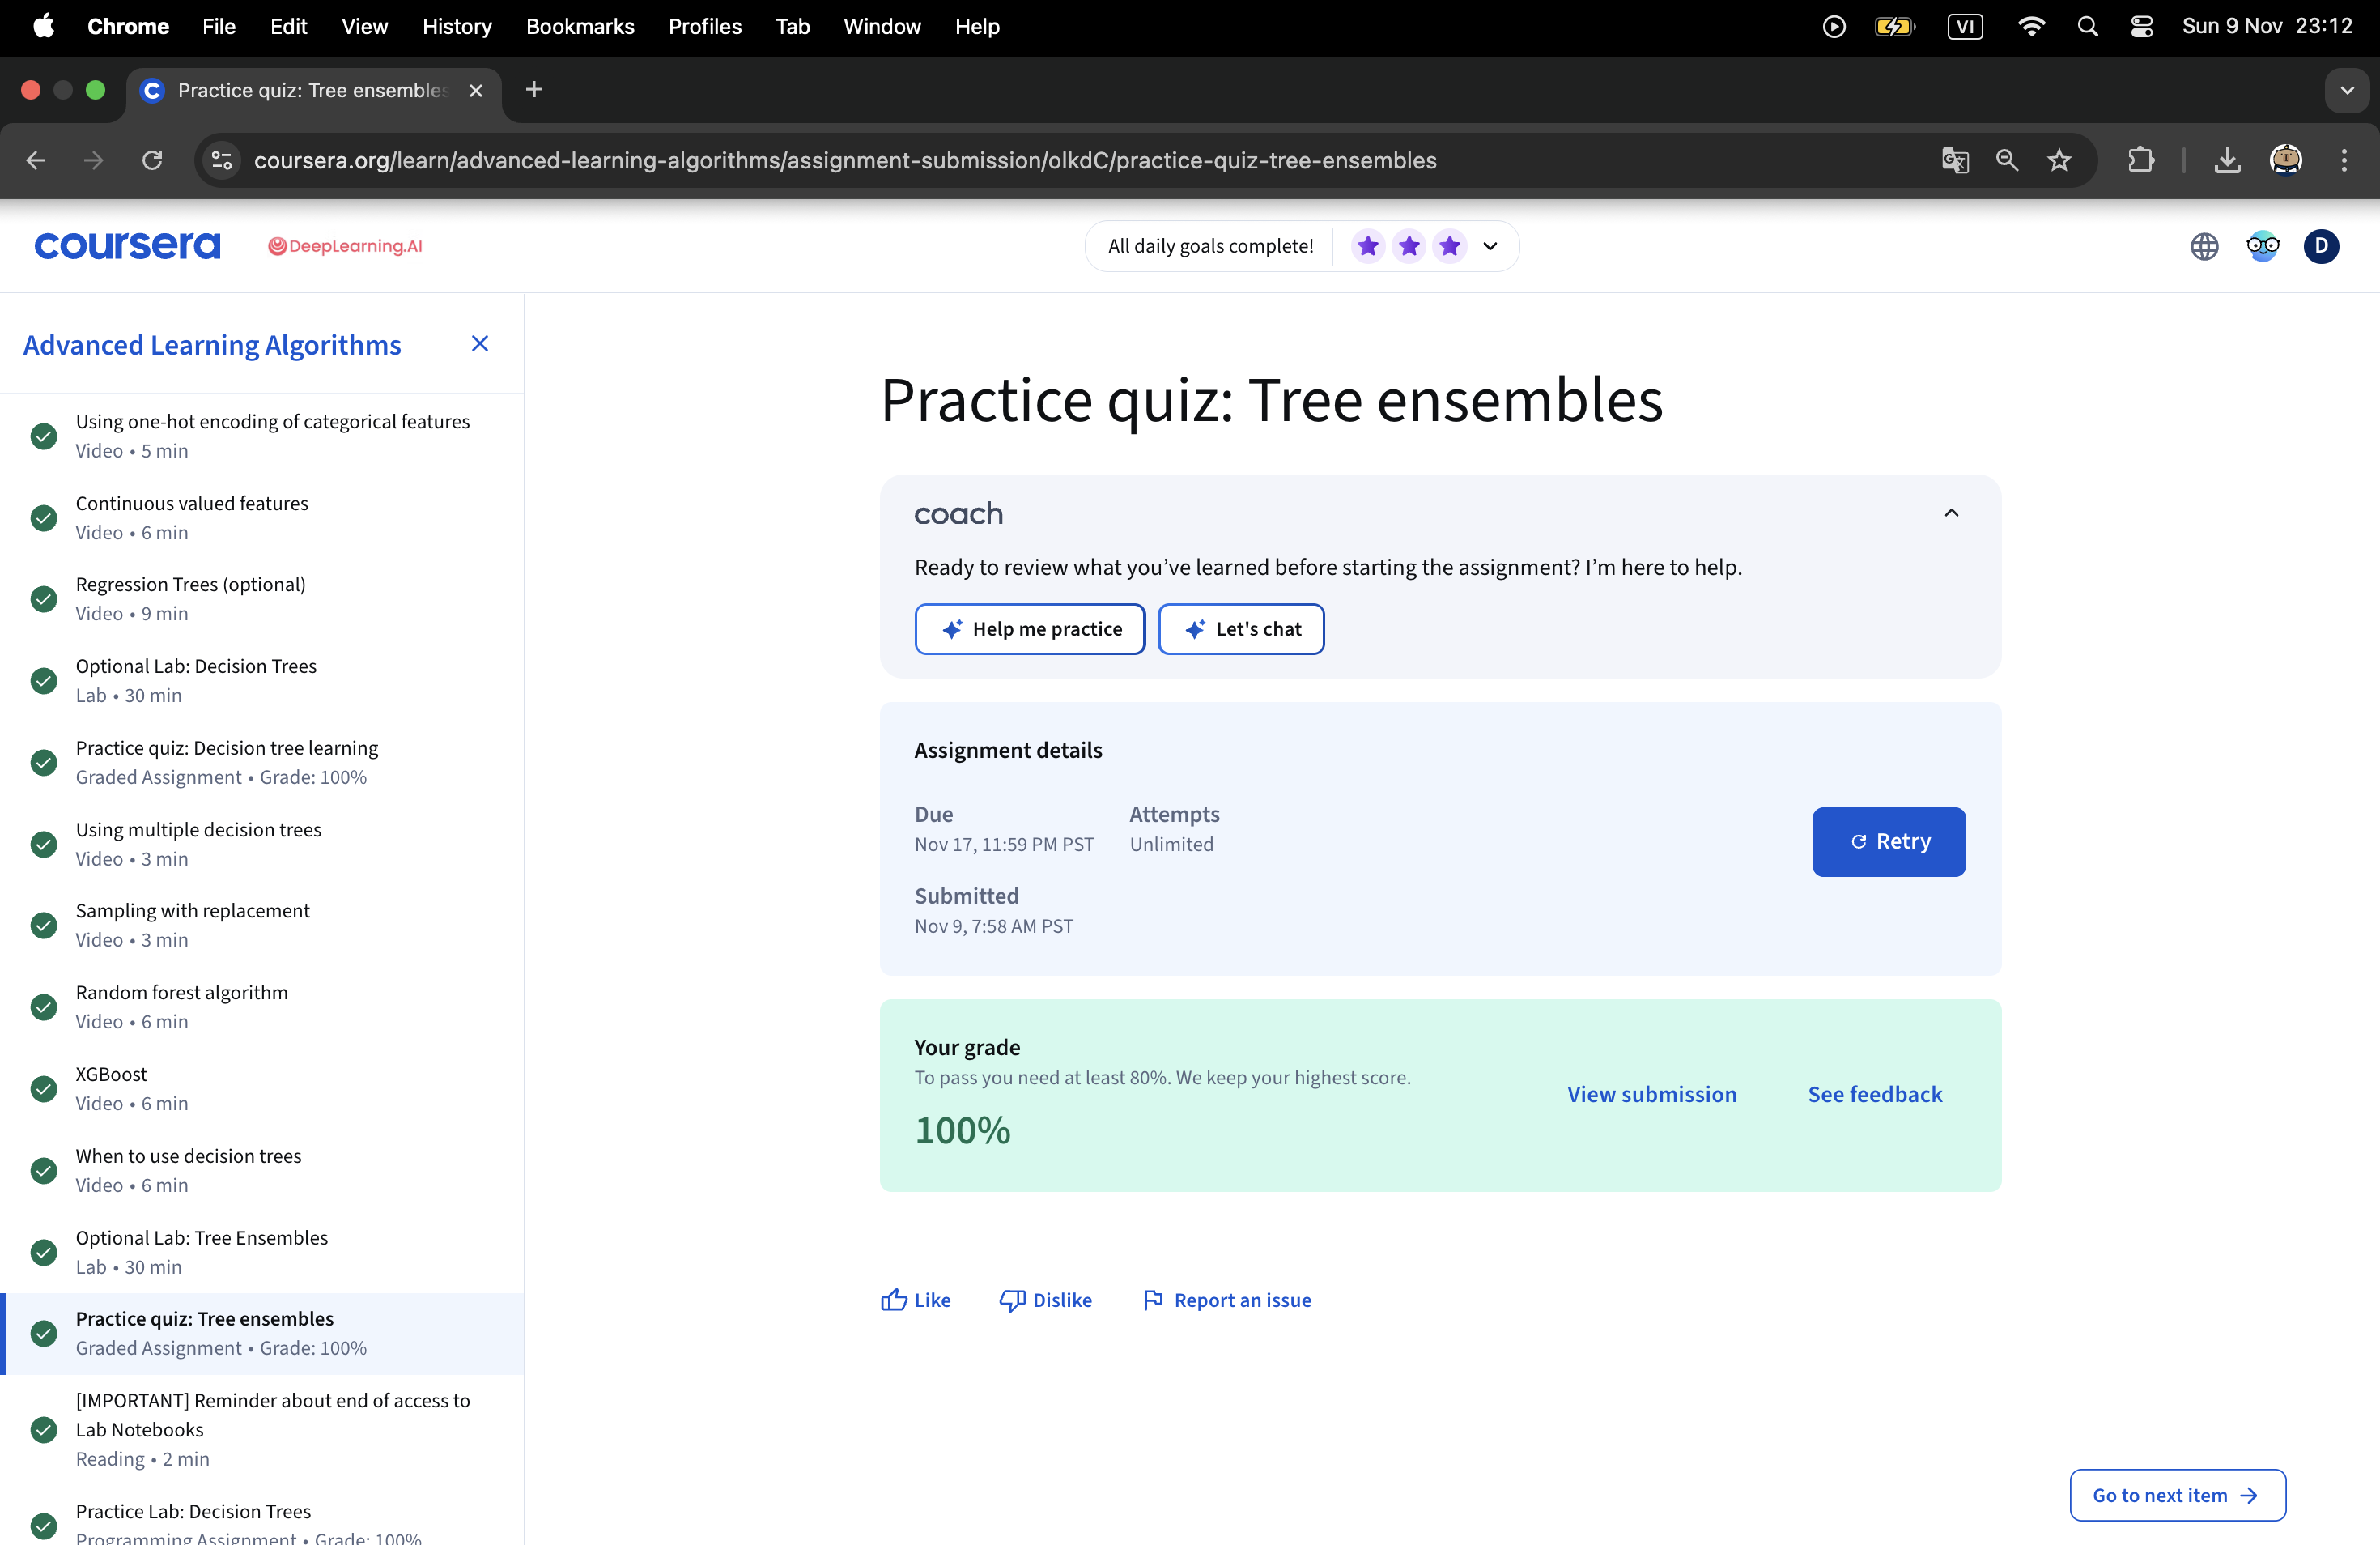
\includegraphics[scale=0.25]{Image/c2_w4_q3.png}
    \caption{Completed Graded Assignment 3 (Tree ensembles)}
\end{figure}


\begin{figure}[H]
    \centering
    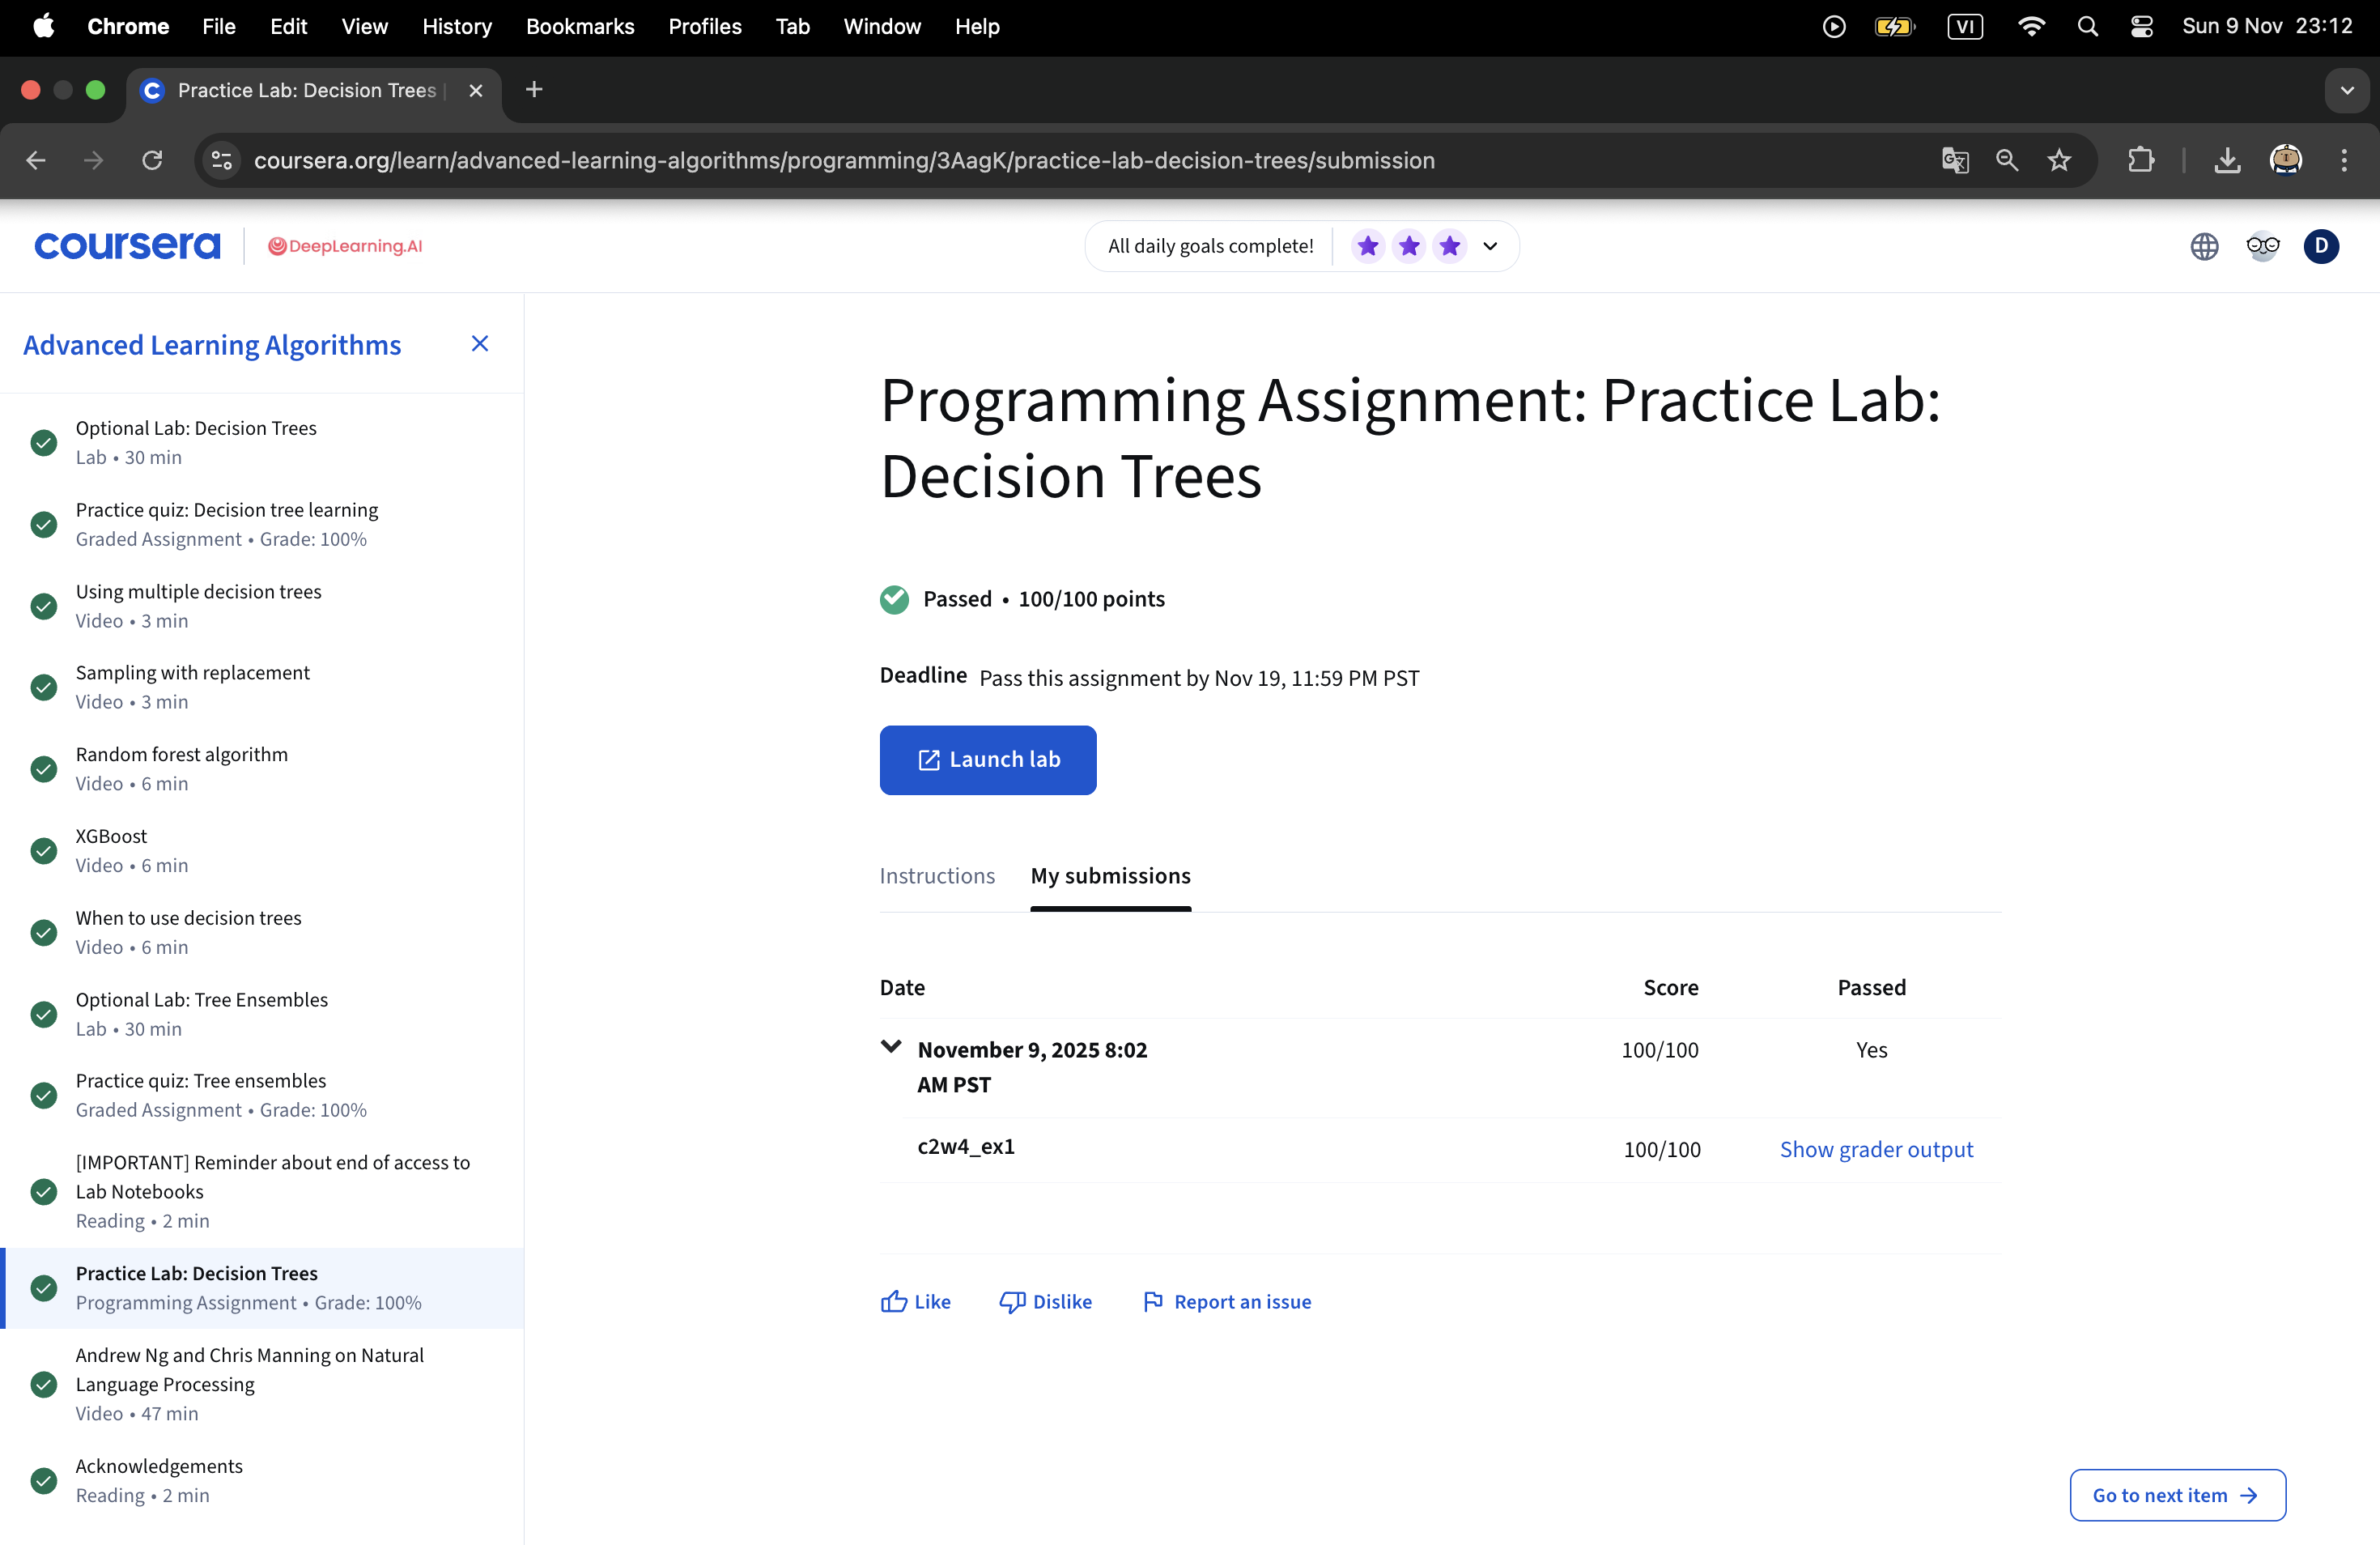
\includegraphics[scale=0.25]{Image/c2_w4_q4.png}
    \caption{Completed Programming Assignment (Decision Trees)}
\end{figure}

\subsection{Certificate for Completion}
\begin{figure}[H]
    \centering
    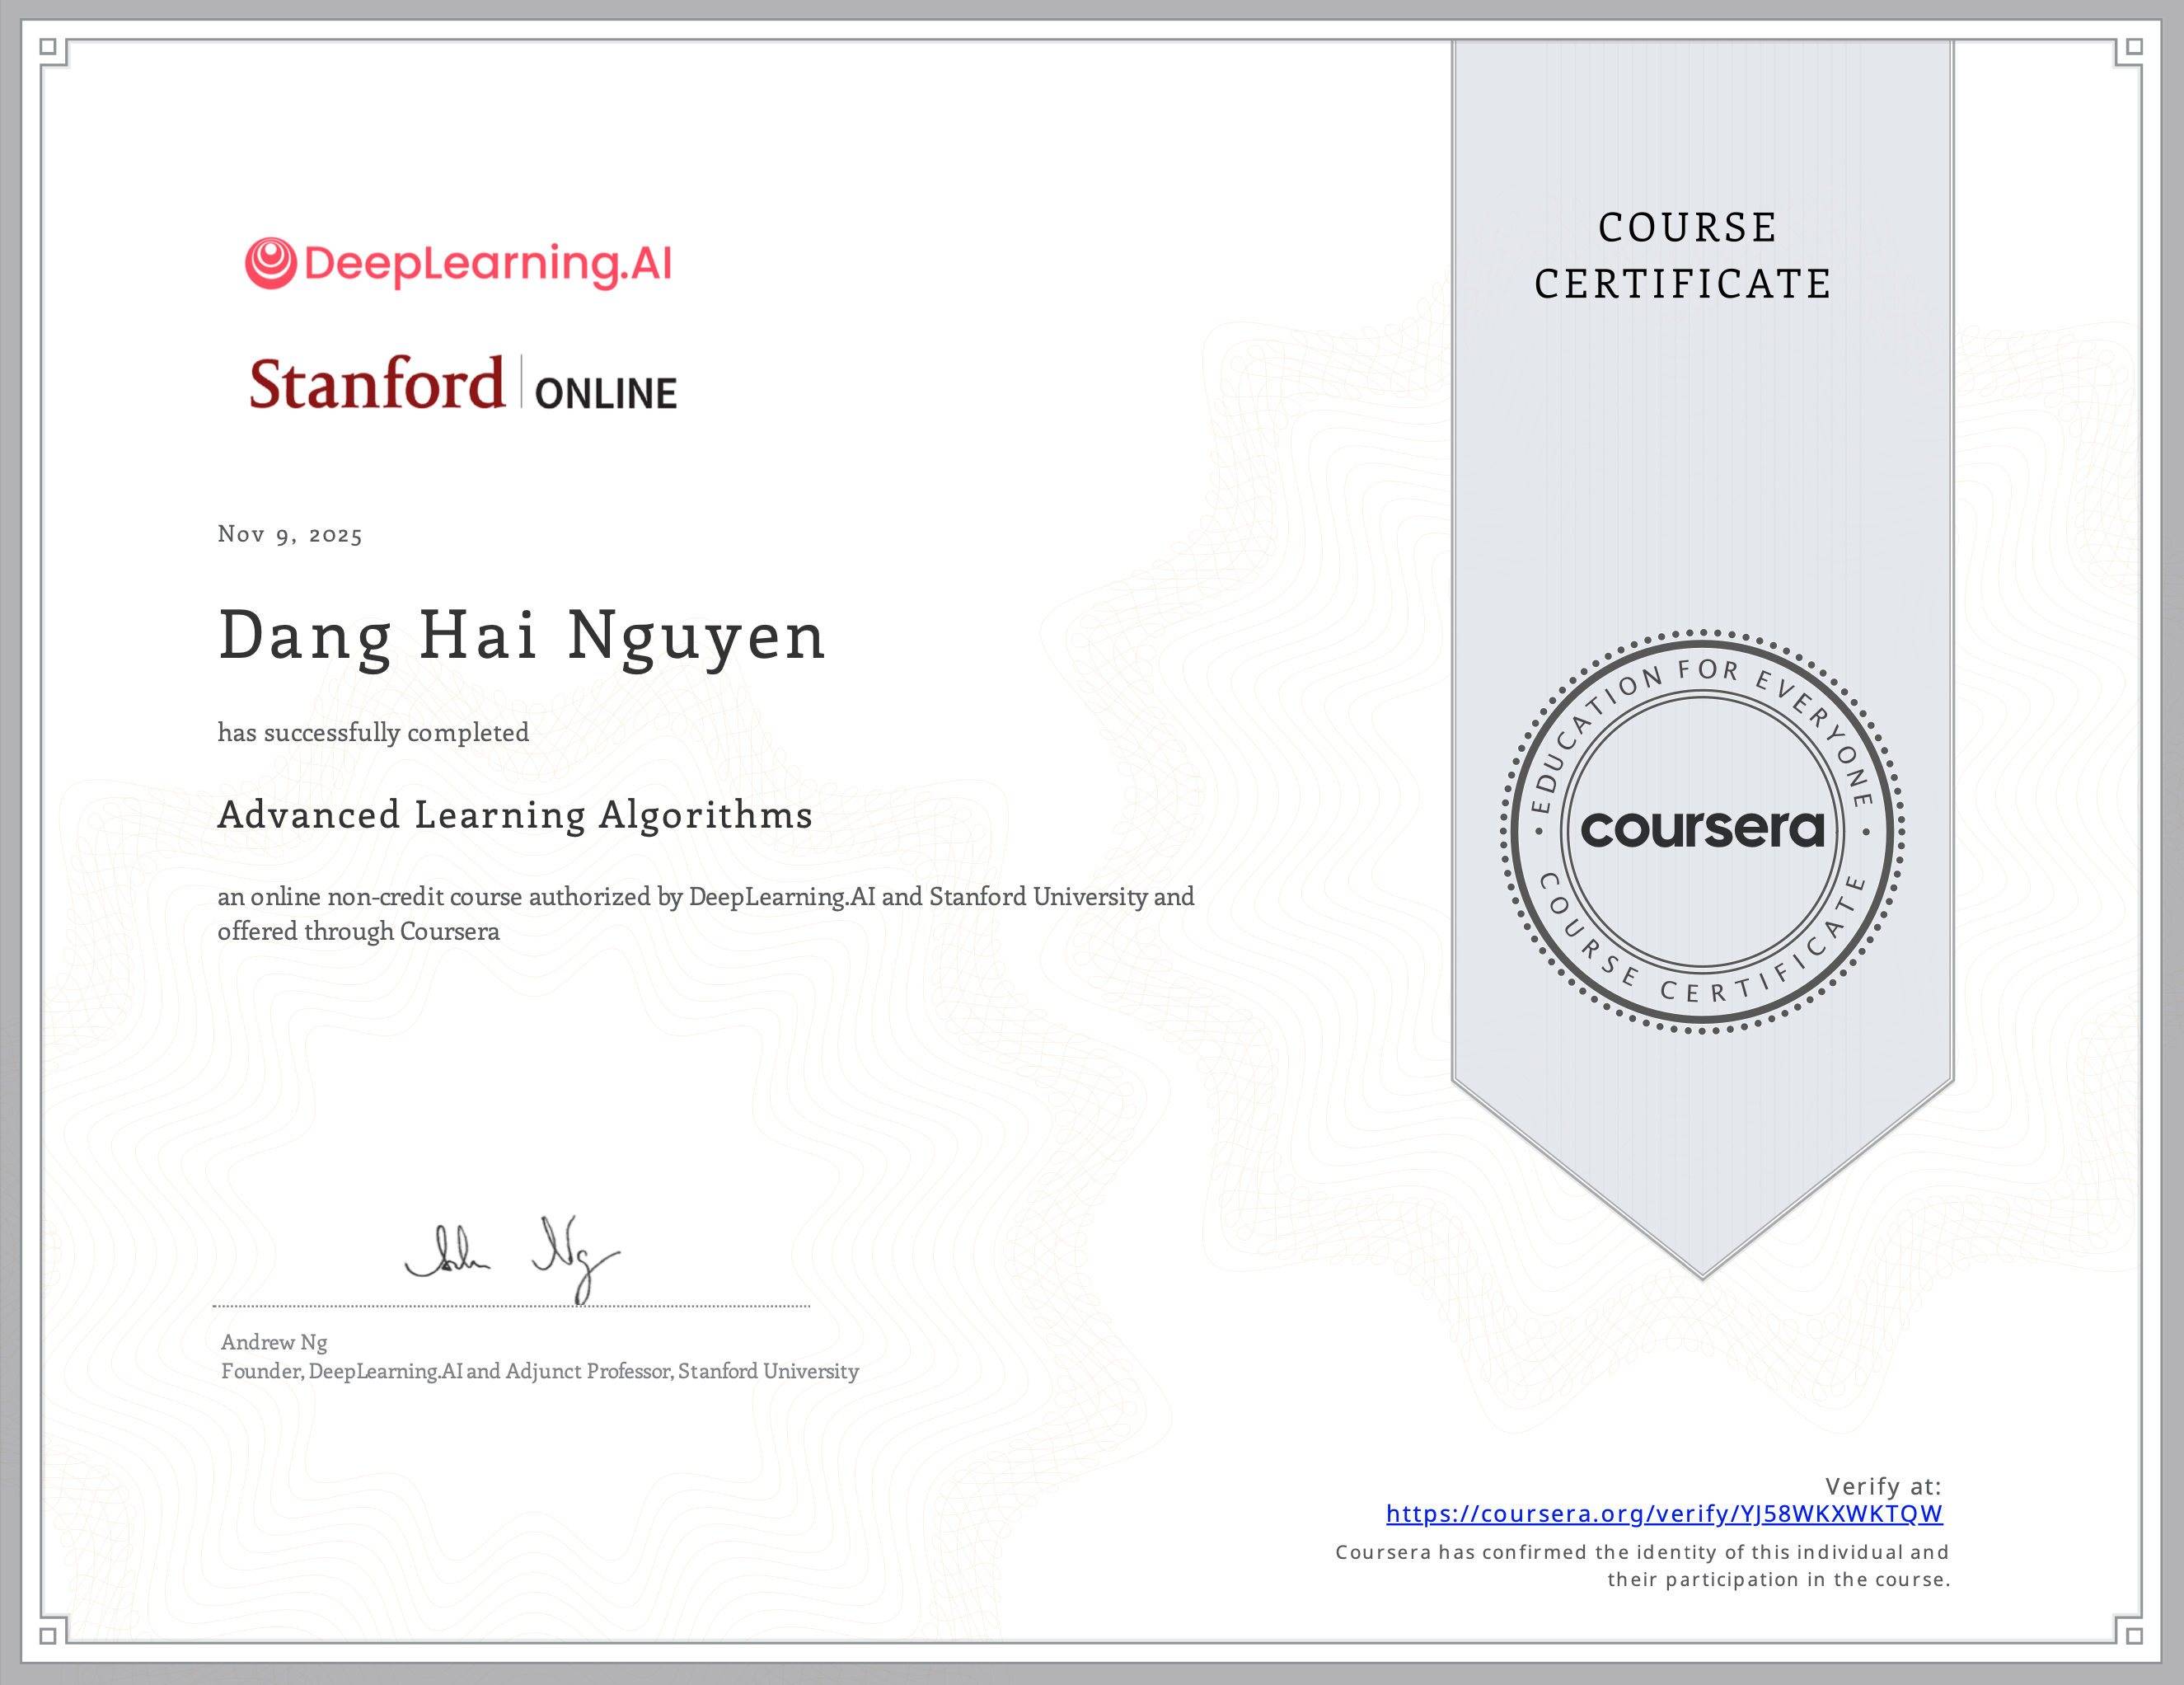
\includegraphics[scale=0.25]{Image/c2_certi.png}
    \caption{Certificate of completion for the course \textit{Advanced Learning Algorithms}.}
\end{figure}


%----------------------------------------
\section{Unsupervised Learning, Recommenders, and Reinforcement Learning}
%----------------------------------------

This final course bridges the gap between standard supervised prediction and autonomous decision-making. It explores how machines uncover hidden patterns in unlabeled data, personalize user experiences through recommendation engines, and learn optimal strategies through interaction with dynamic environments.

\begin{figure}[H]
    \centering
    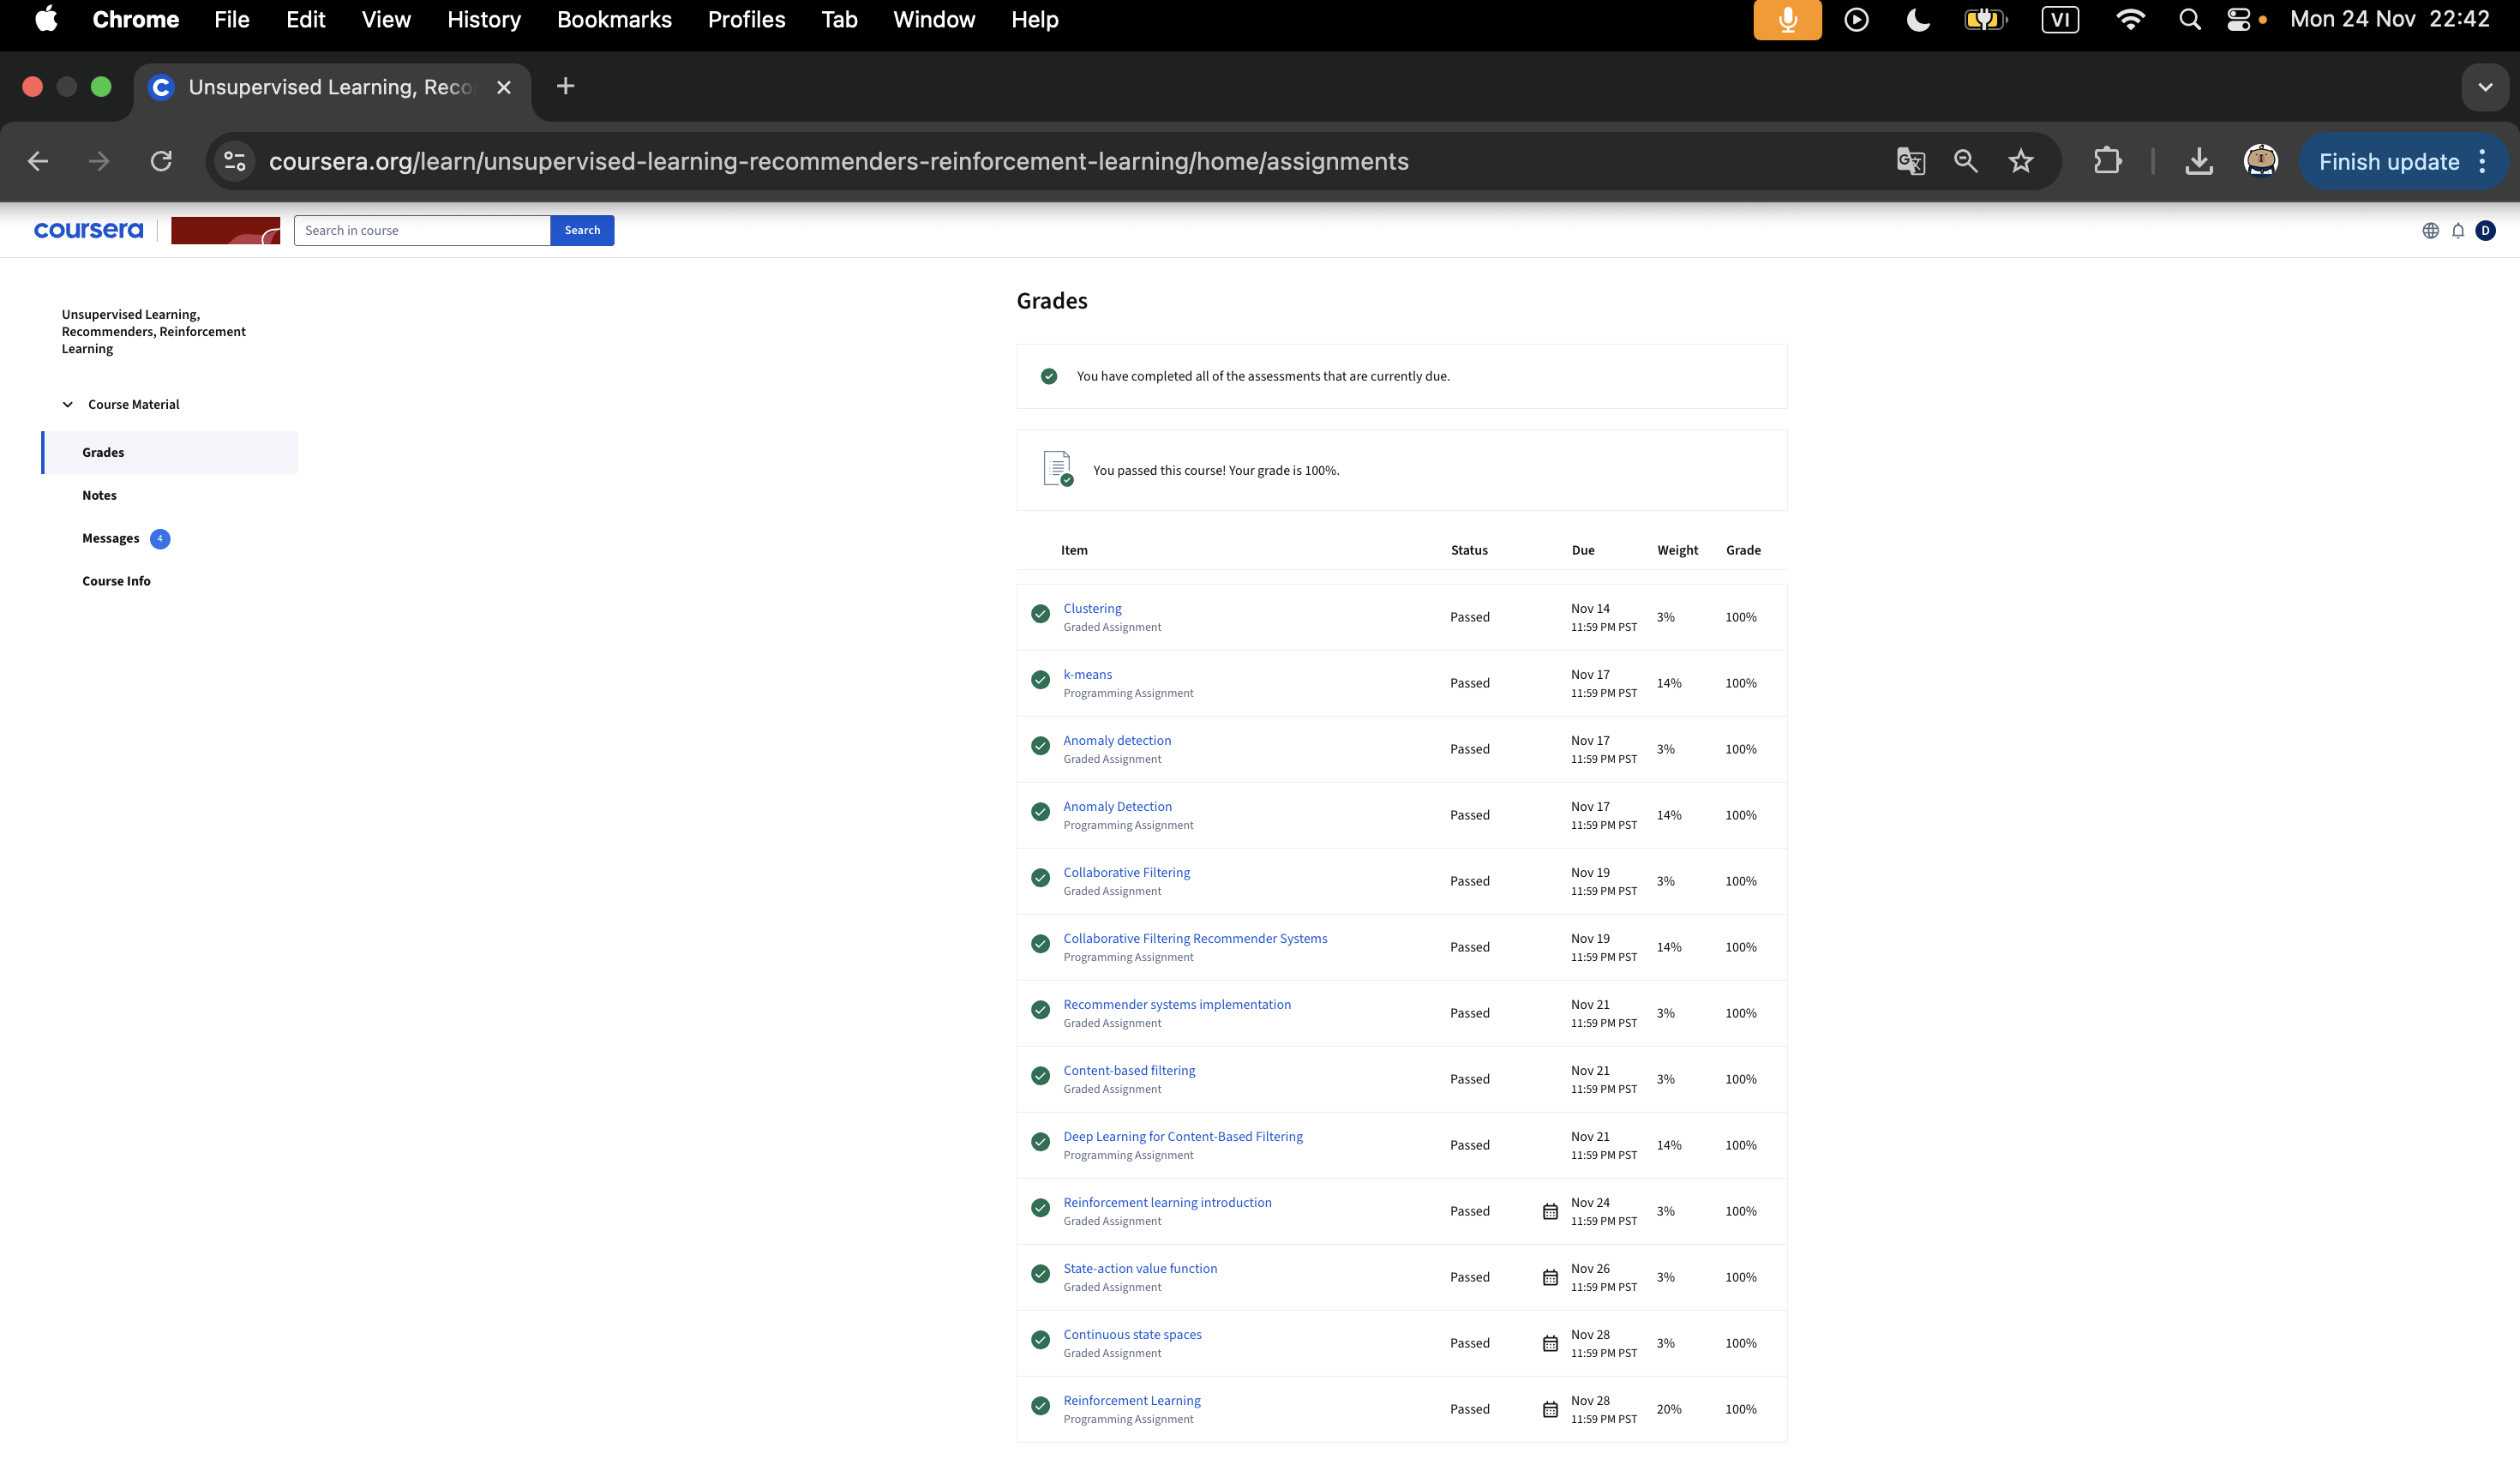
\includegraphics[scale=0.2]{Image/c3.png}
    \caption{Course 3 Completion Certificate}
\end{figure}

%----------------------------------------
\subsection{Week 1: Unsupervised Learning \& Anomaly Detection}
%----------------------------------------

\subsubsection{Key Insights and Learnings}

This module focused on algorithms that derive structure from data without pre-existing labels, essential for exploratory data analysis, pattern recognition, and system monitoring.

\begin{itemize}
    \item \textbf{Clustering with K-Means:} Learned to partition data into $k$ distinct groups by minimizing the variance within each cluster. 
    \begin{itemize}
        \item Applied the \textit{Elbow Method} to determine the optimal number of clusters ($k$) based on the distortion cost function.
        \item \textbf{Applications:} Market segmentation, document organization, and astronomical data analysis.
    \end{itemize}

    \item \textbf{Anomaly Detection:} Constructed probabilistic models using Gaussian (Normal) distribution to identify outliers or unusual events in a dataset.
    \begin{itemize}
        \item \textbf{Technique:} Estimating parameters ($\mu, \sigma^2$) to flag data points with very low probability density ($p(x) < \epsilon$).
        \item \textbf{Applications:} Fraud detection in finance, quality control in manufacturing, and server monitoring.
    \end{itemize}
    
    \item \textbf{Dimensionality Reduction (PCA):} Utilized \textbf{Principal Component Analysis} to compress data while retaining critical information. By finding underlying axes of maximum variance, PCA reduces feature dimensionality, which aids in data visualization (2D/3D) and improves the efficiency of supervised learning models.
\end{itemize}

\subsubsection{Learning Evidence}
\begin{figure}[H]
    \centering
    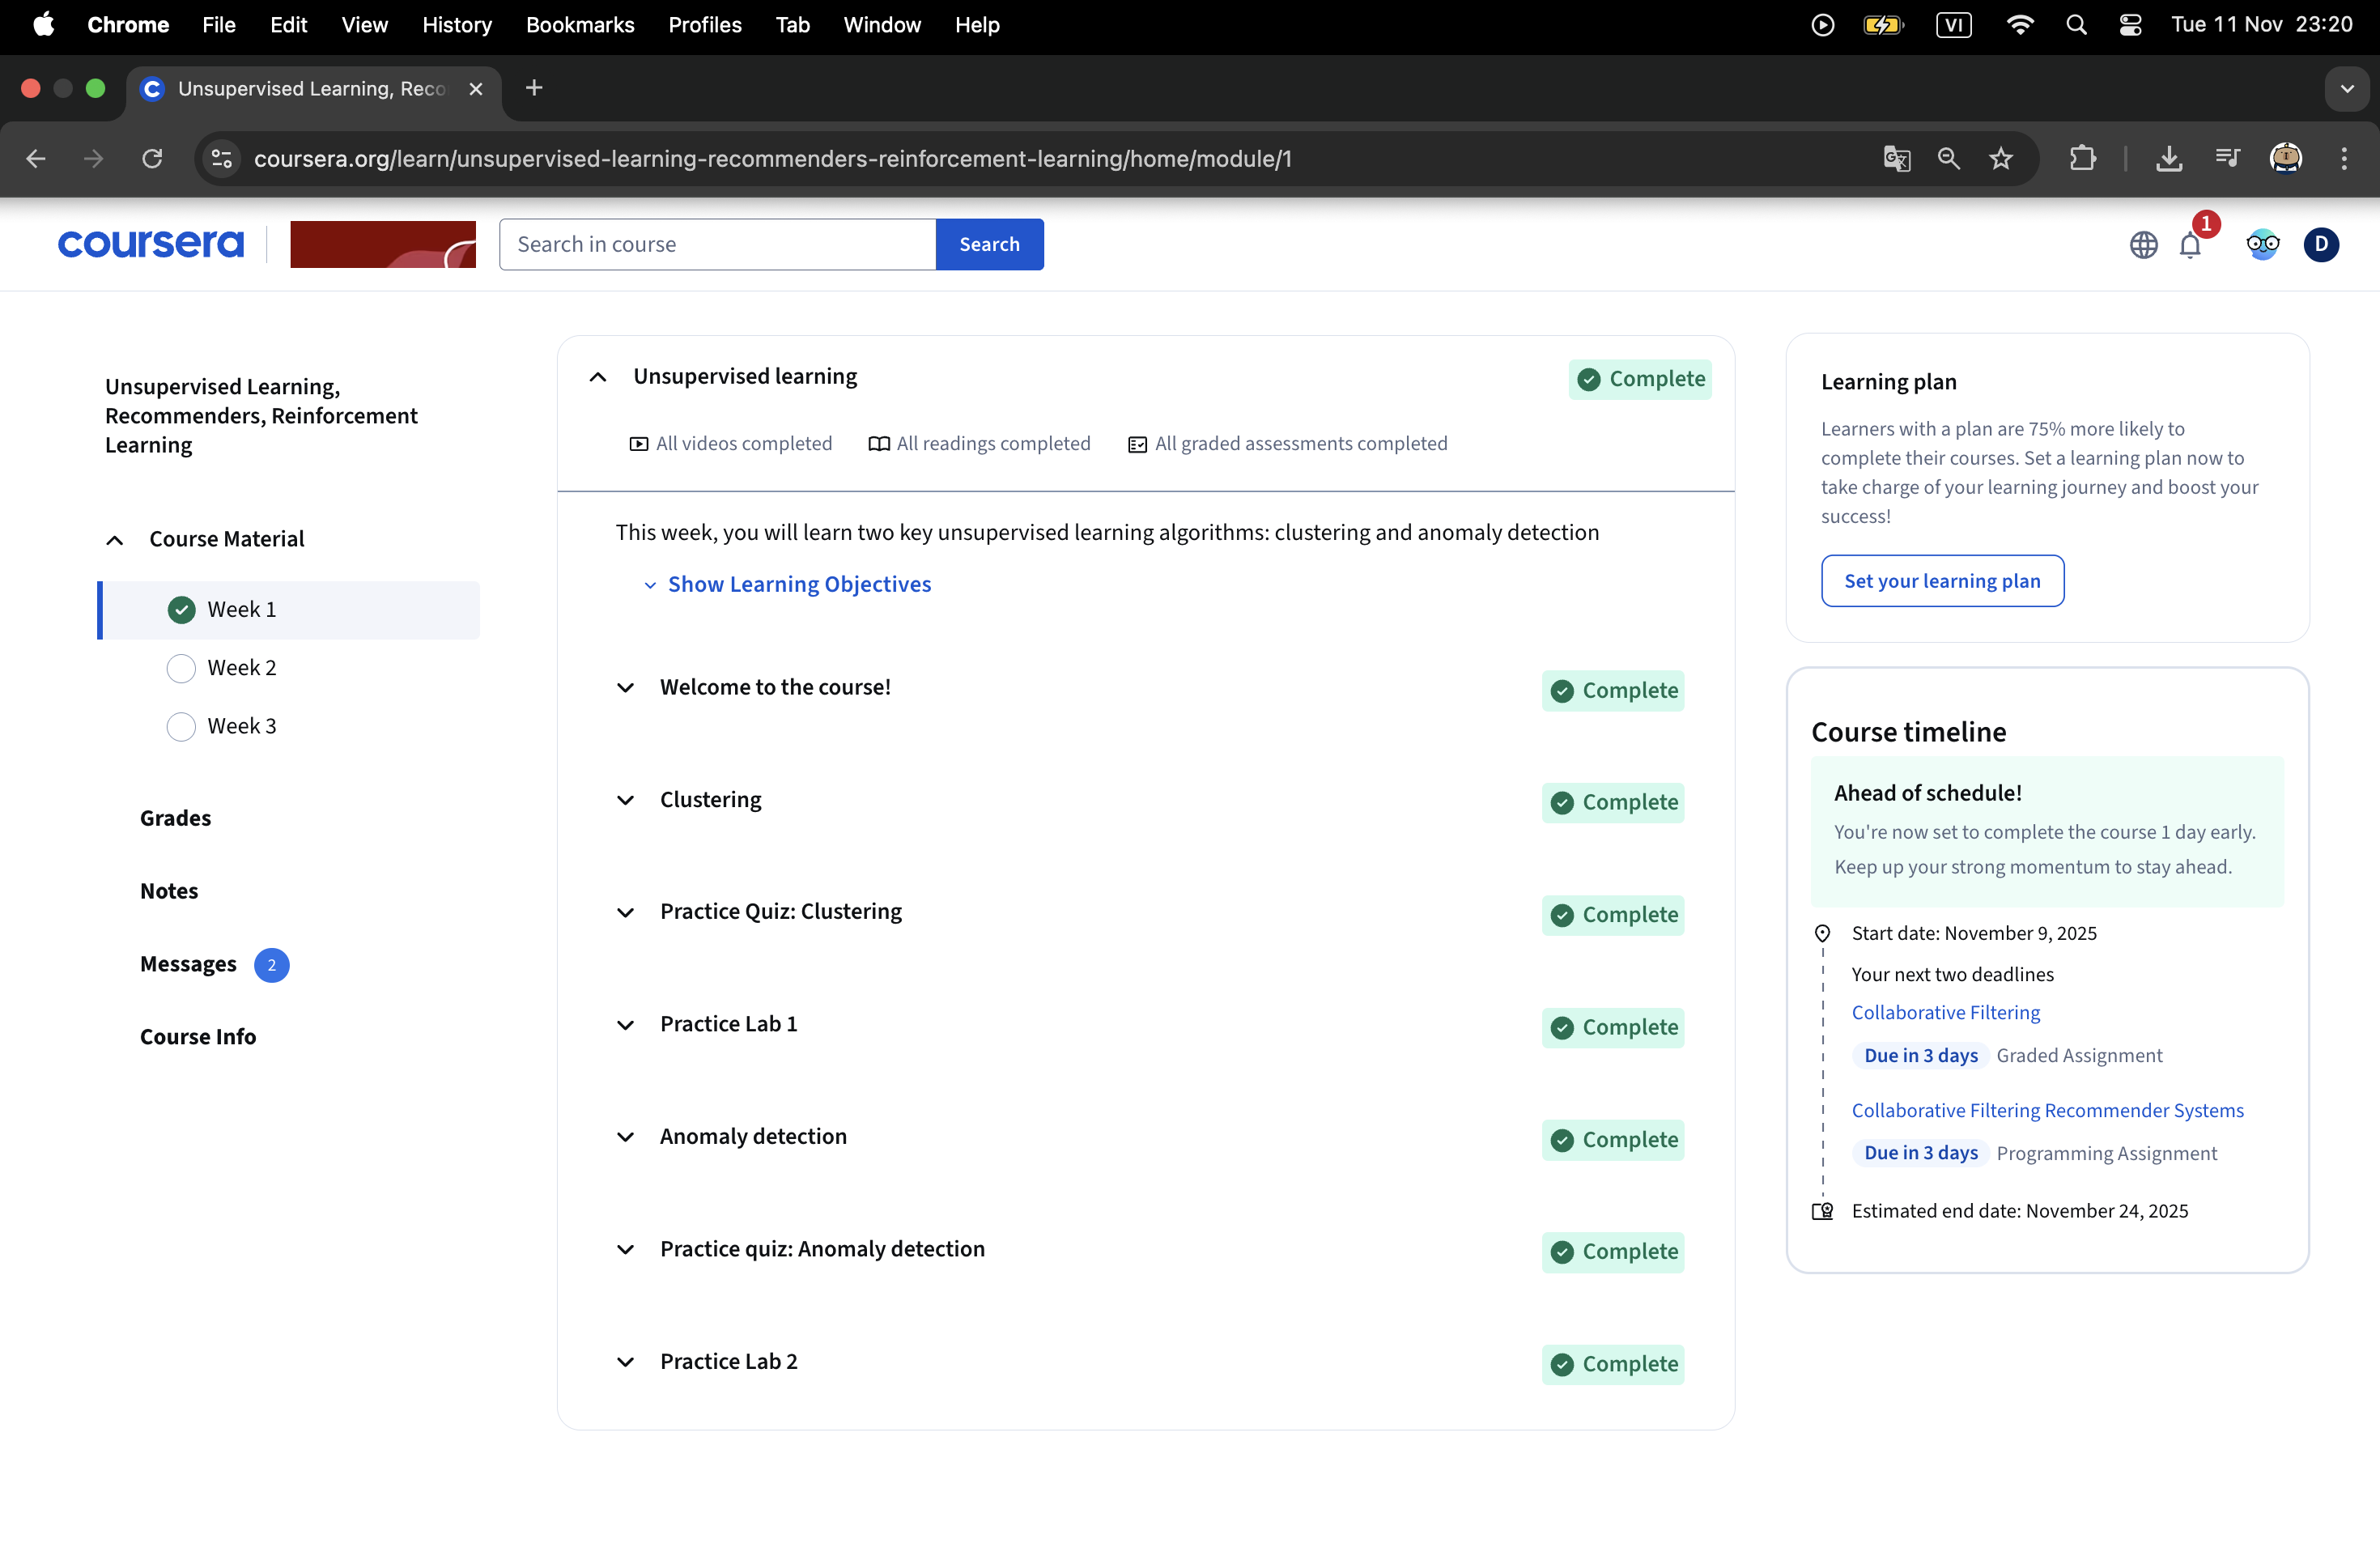
\includegraphics[scale=0.25]{Image/c3_w1.png}
    \caption{Lesson's completed date (11/11/2025)}
\end{figure}

\subsubsection{Graded Assignment Evidence}
\begin{figure}[H]
    \centering
    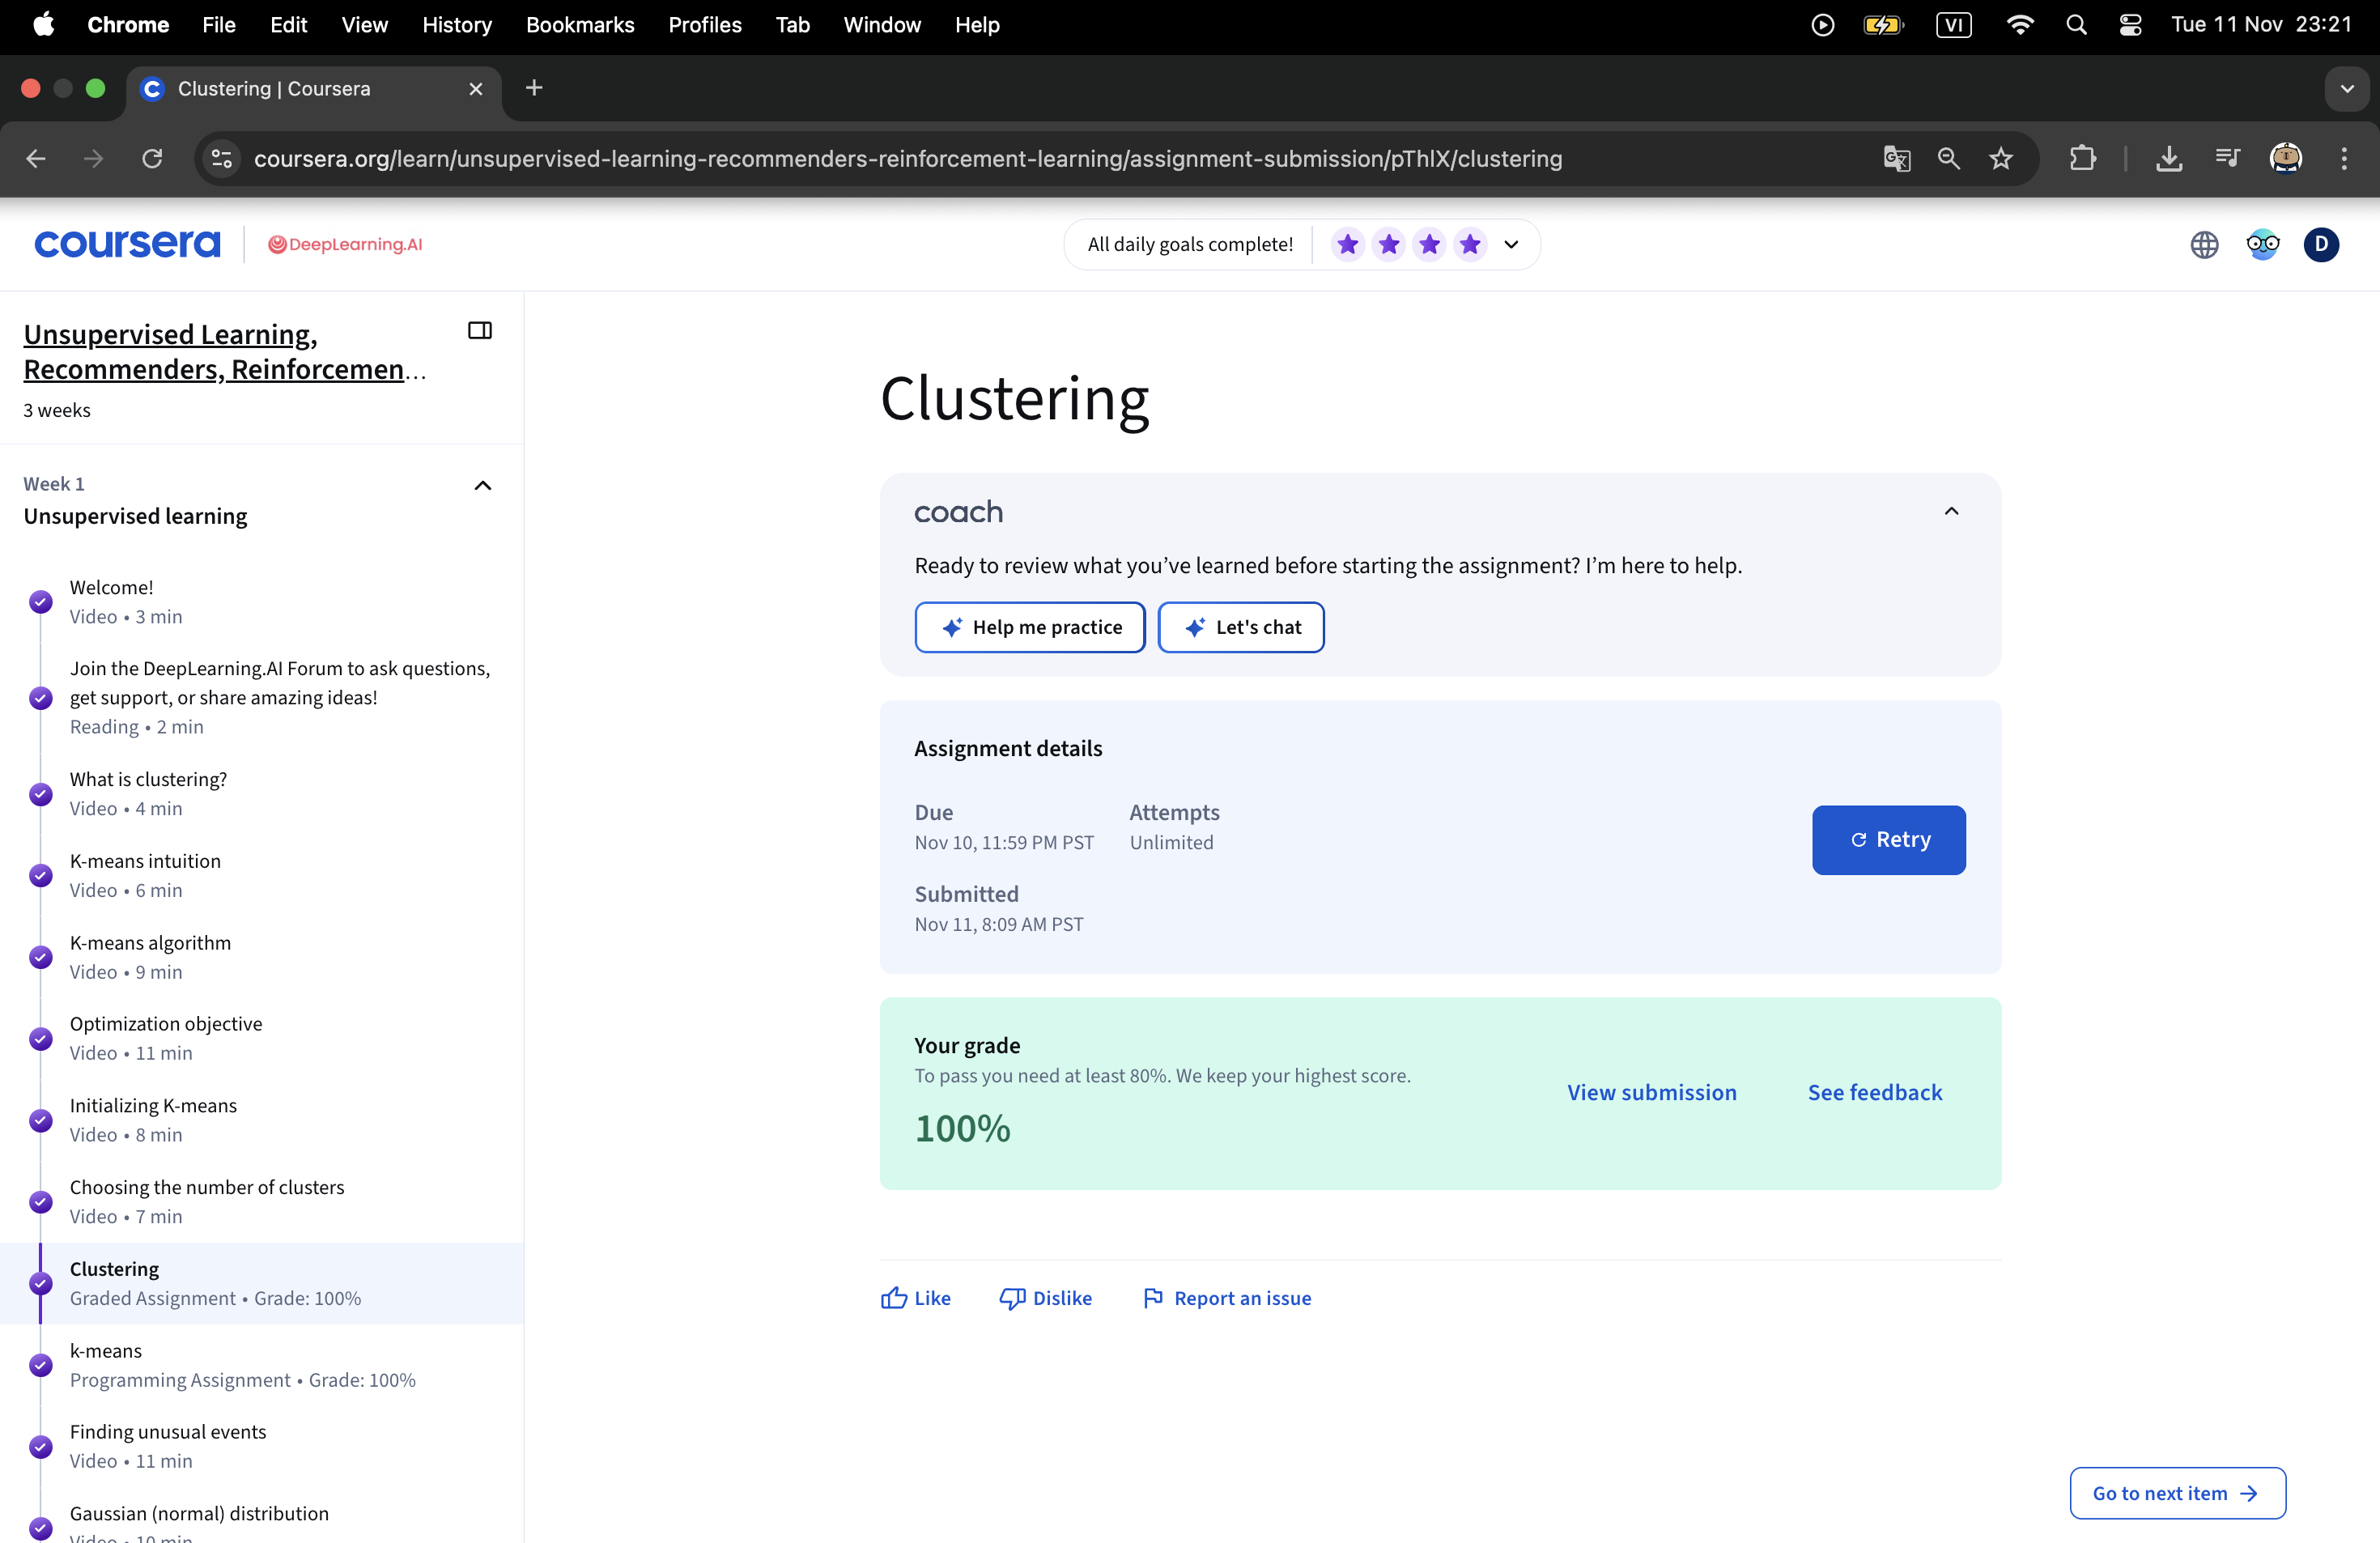
\includegraphics[scale=0.27]{Image/c3_w1_q1.png}
    \caption{Completed Graded Assignment 1 (Clustering)}
\end{figure}

\begin{figure}[H]
    \centering
    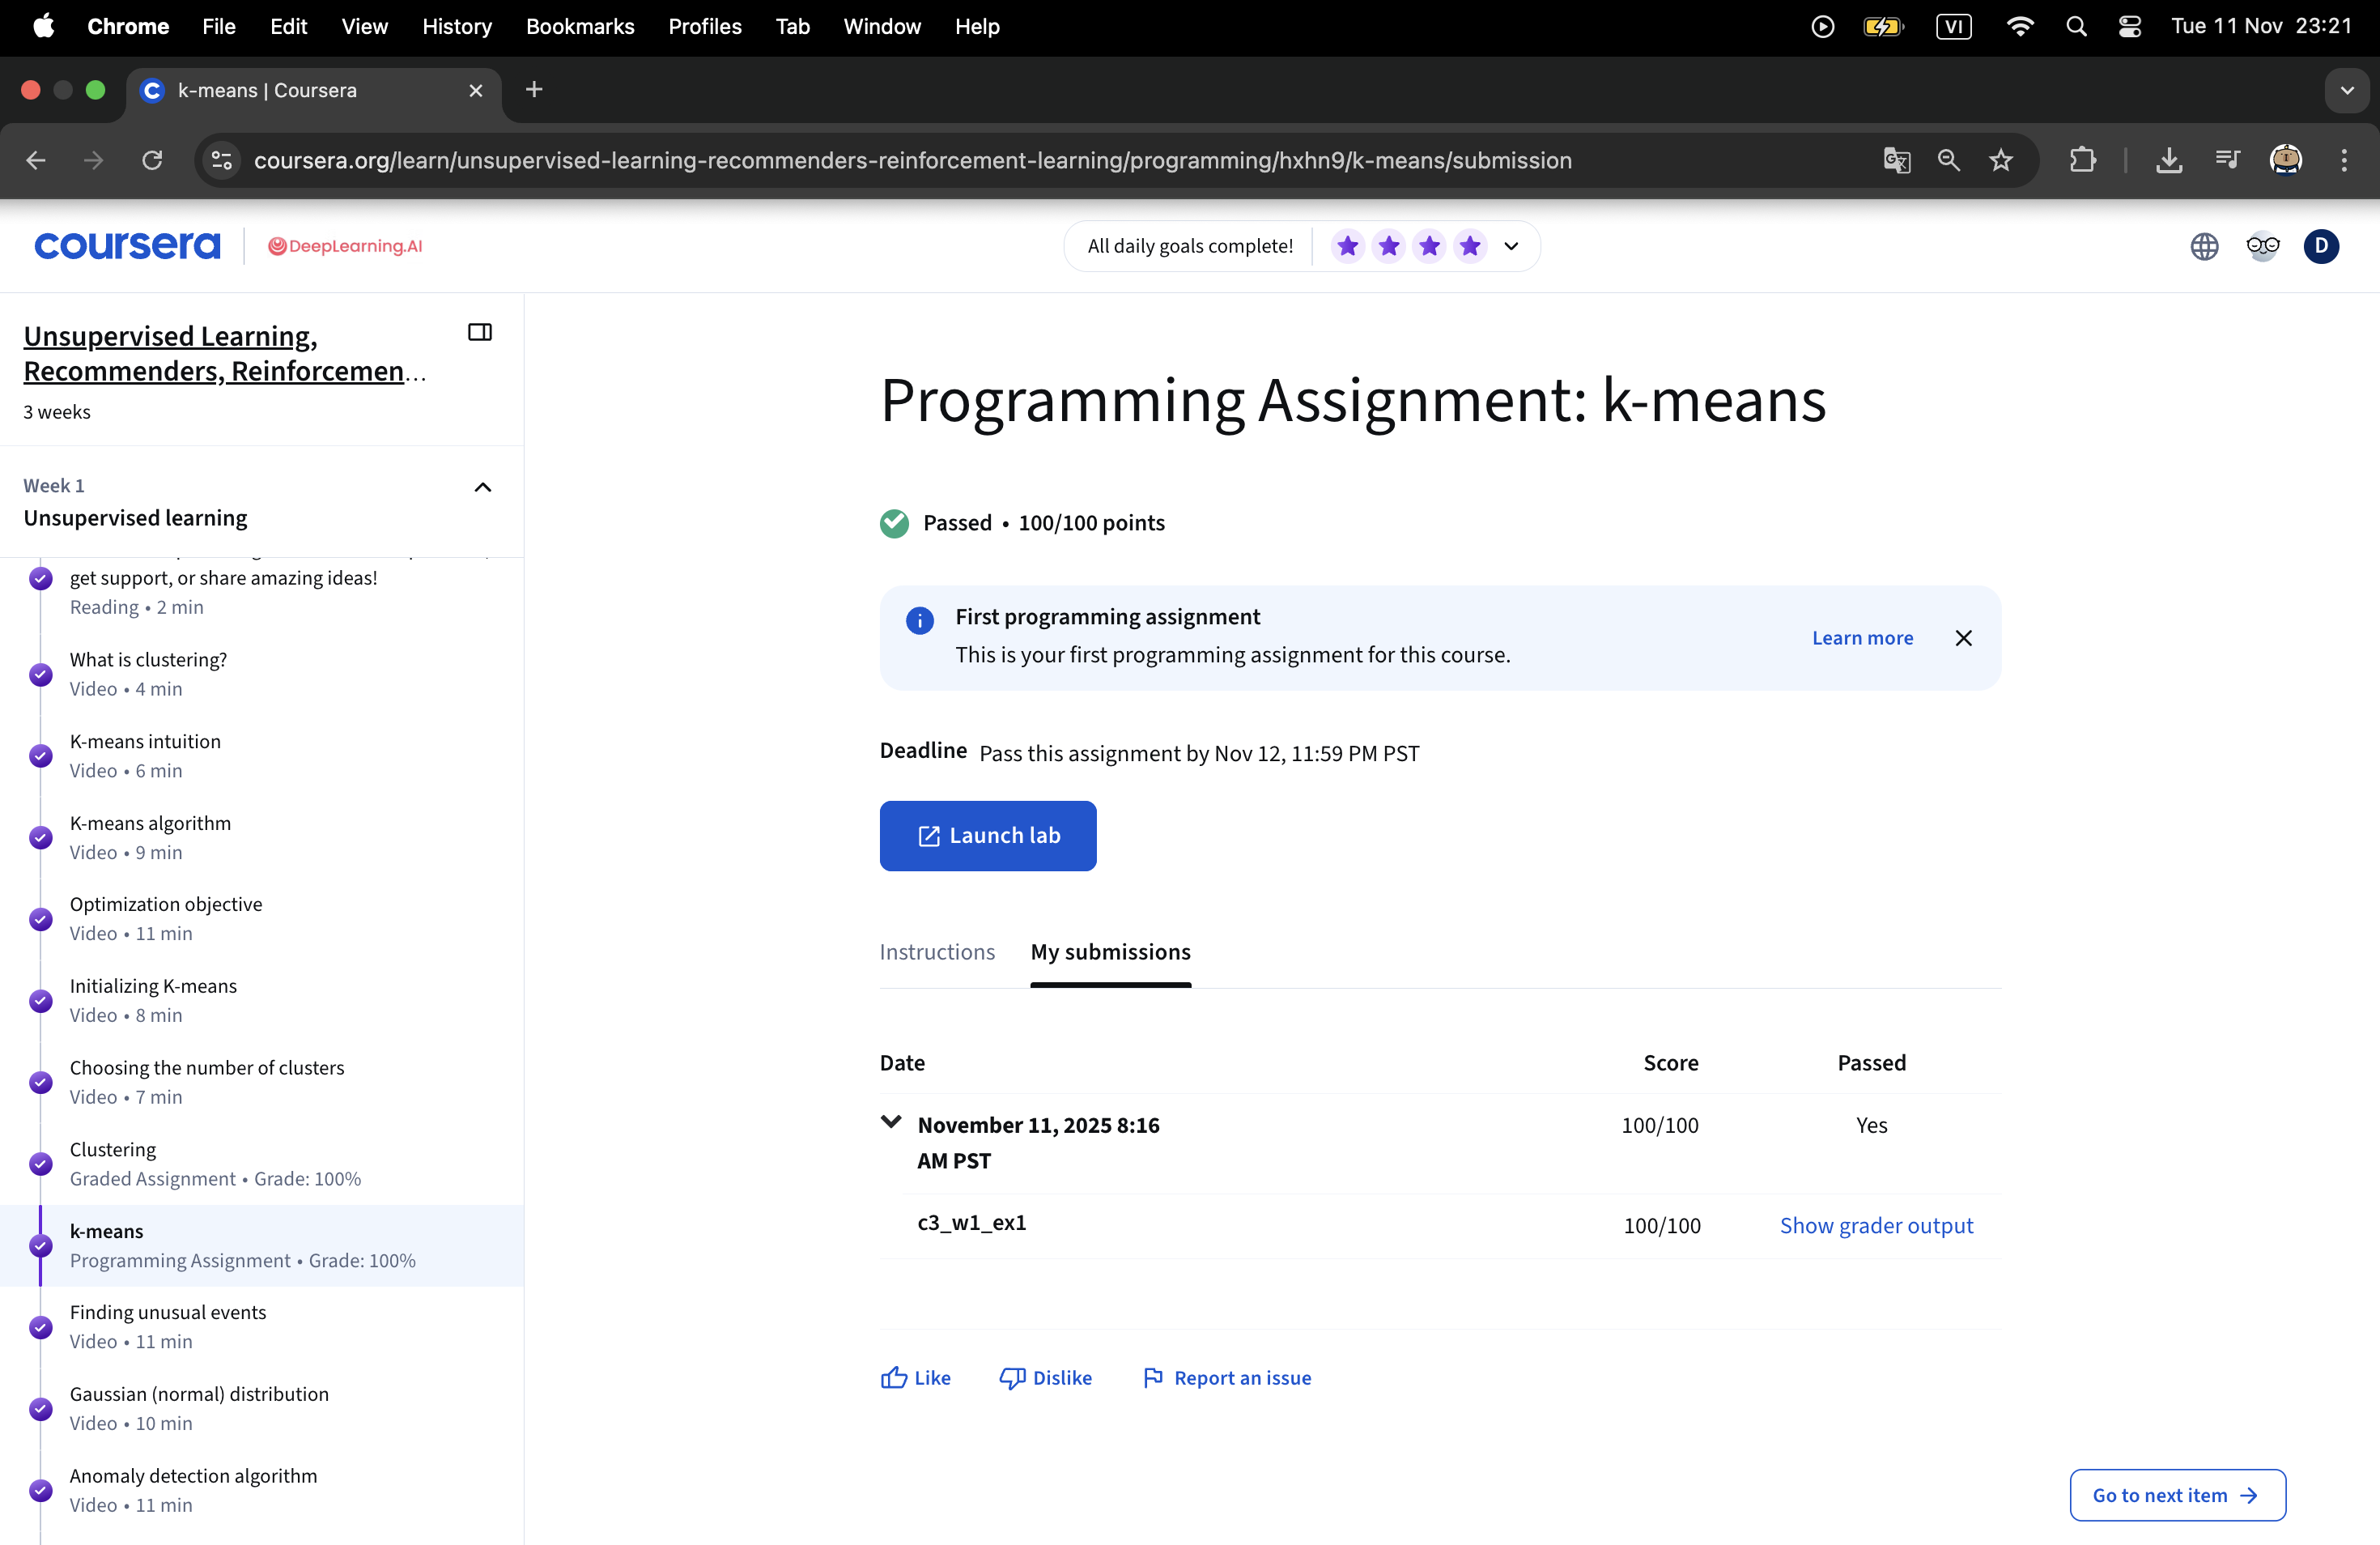
\includegraphics[scale=0.27]{Image/c3_w1_q2.png}
    \caption{Completed Programming Assignment (k-means)}
\end{figure}

\begin{figure}[H]
    \centering
    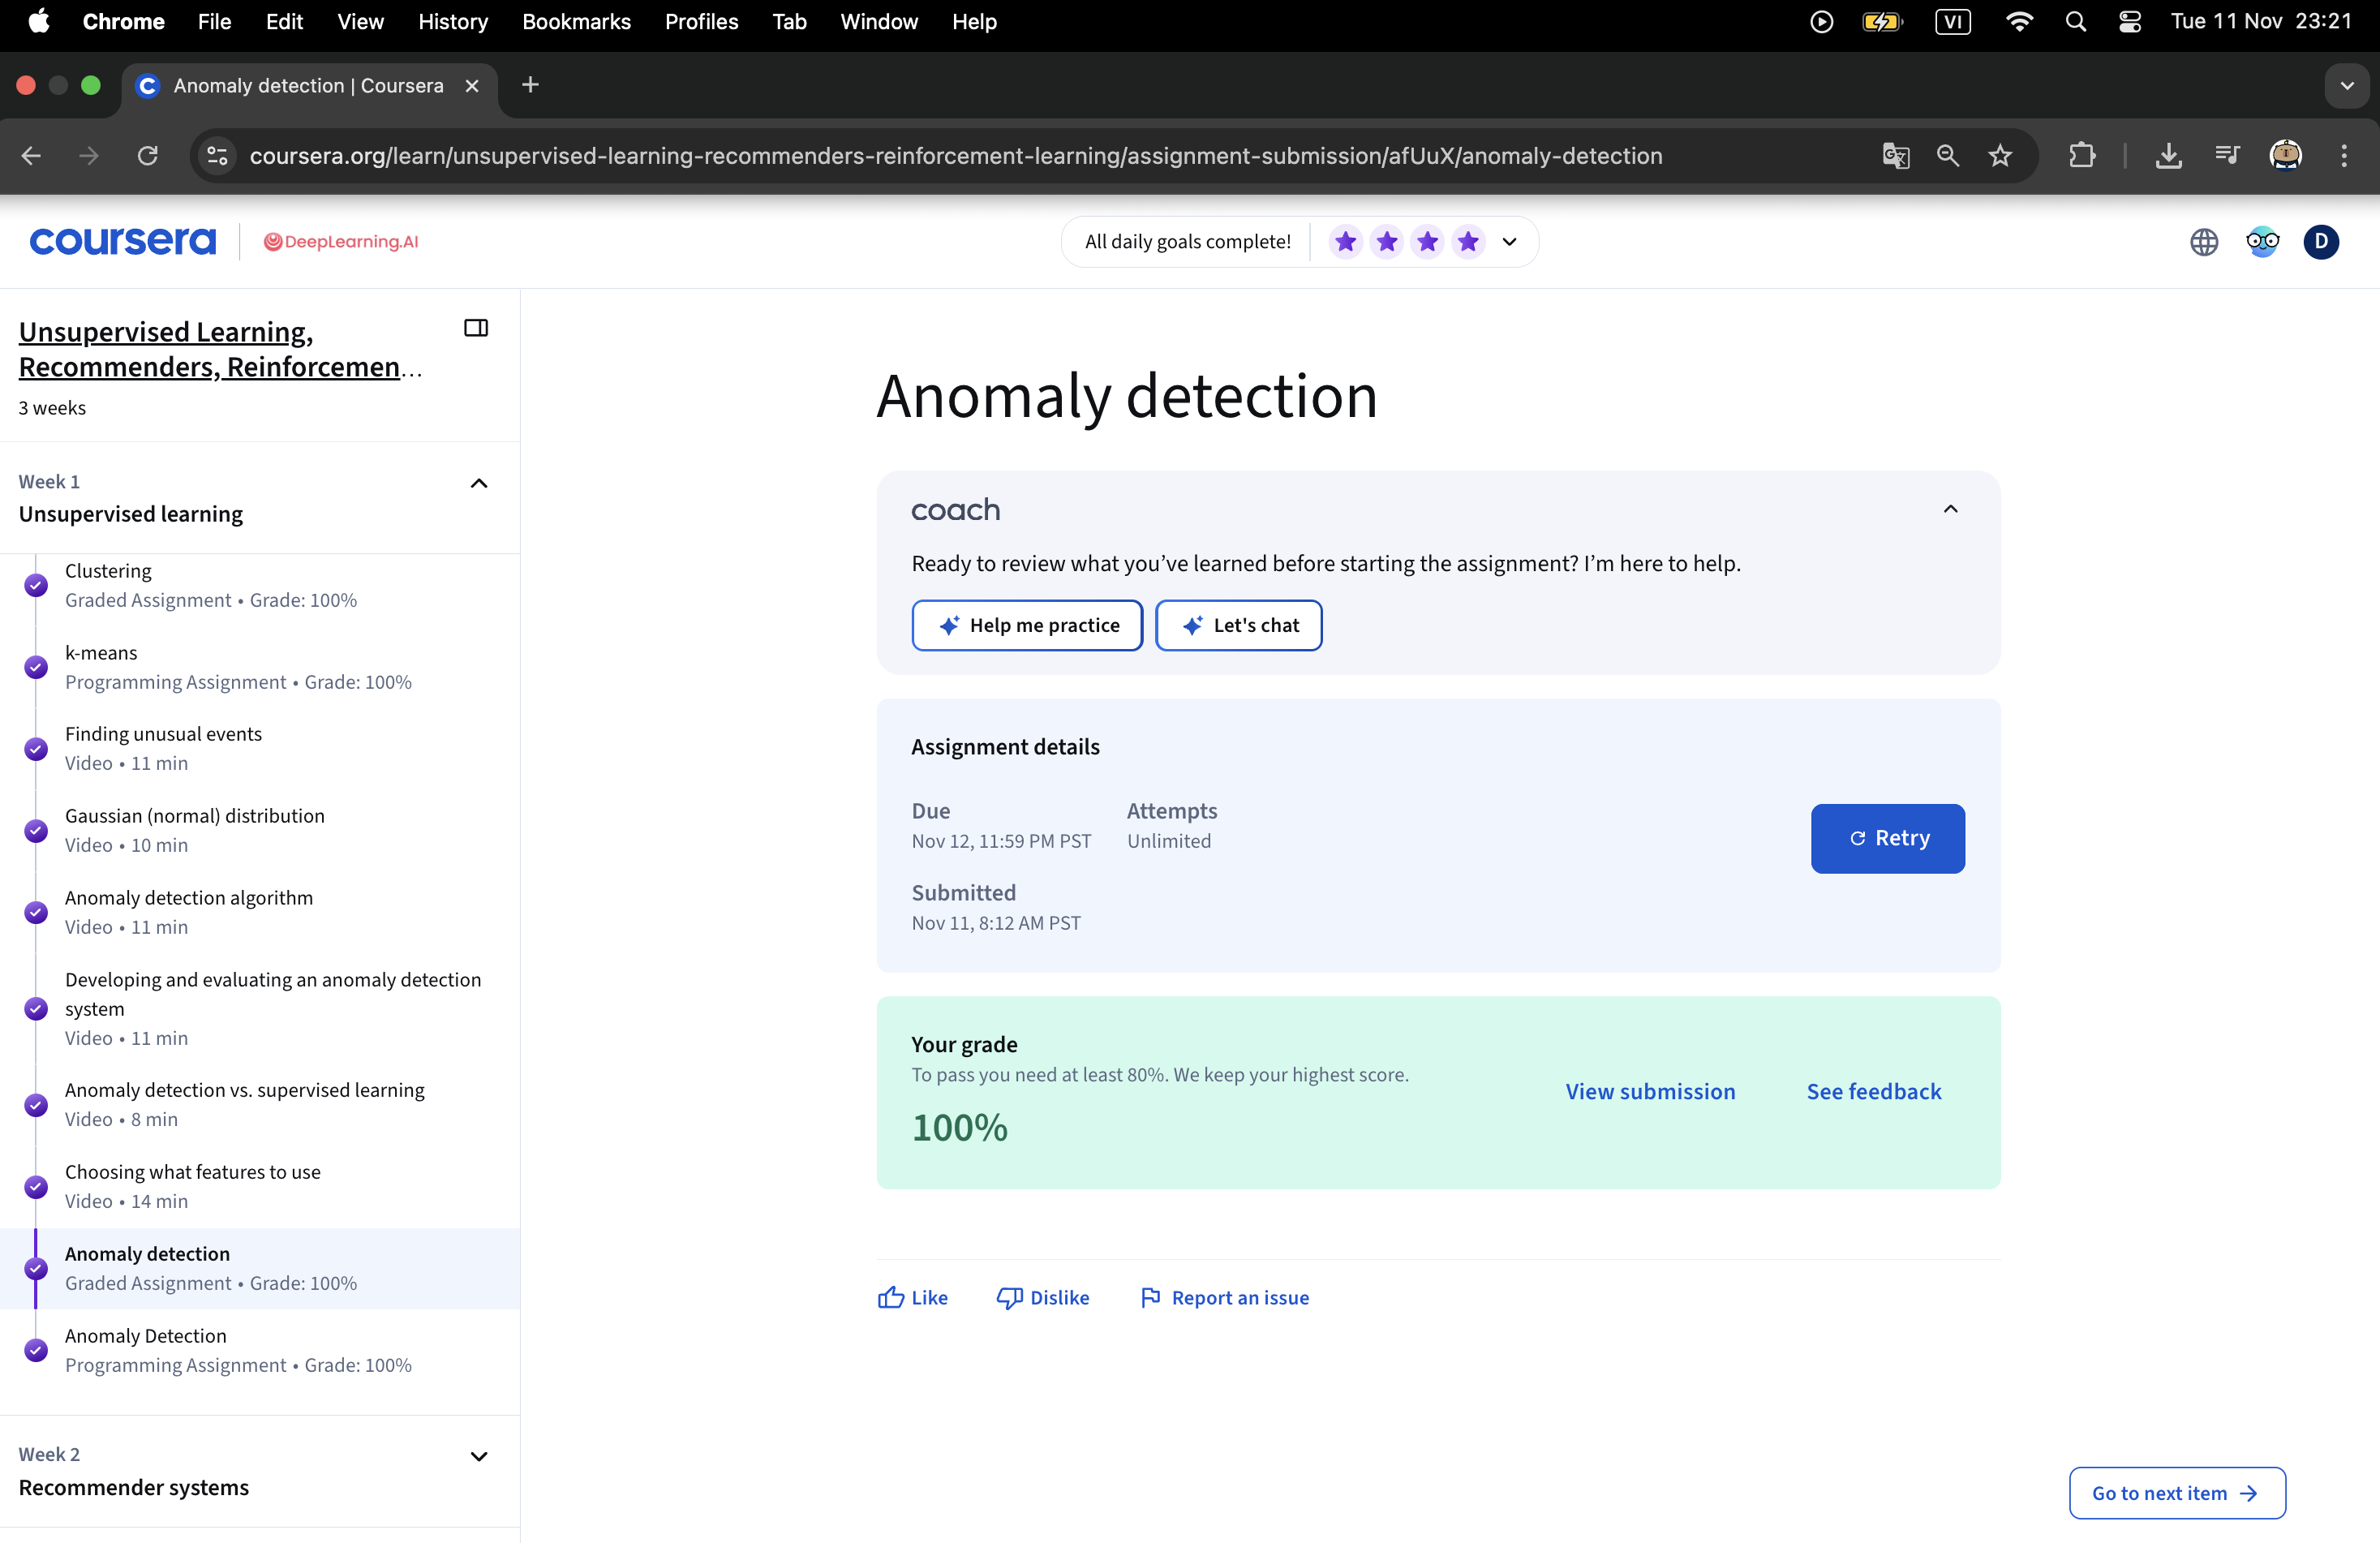
\includegraphics[scale=0.27]{Image/c3_w1_q3.png}
    \caption{Completed Graded Assignment 3 (Anomaly detection)}
\end{figure}


\begin{figure}[H]
    \centering
    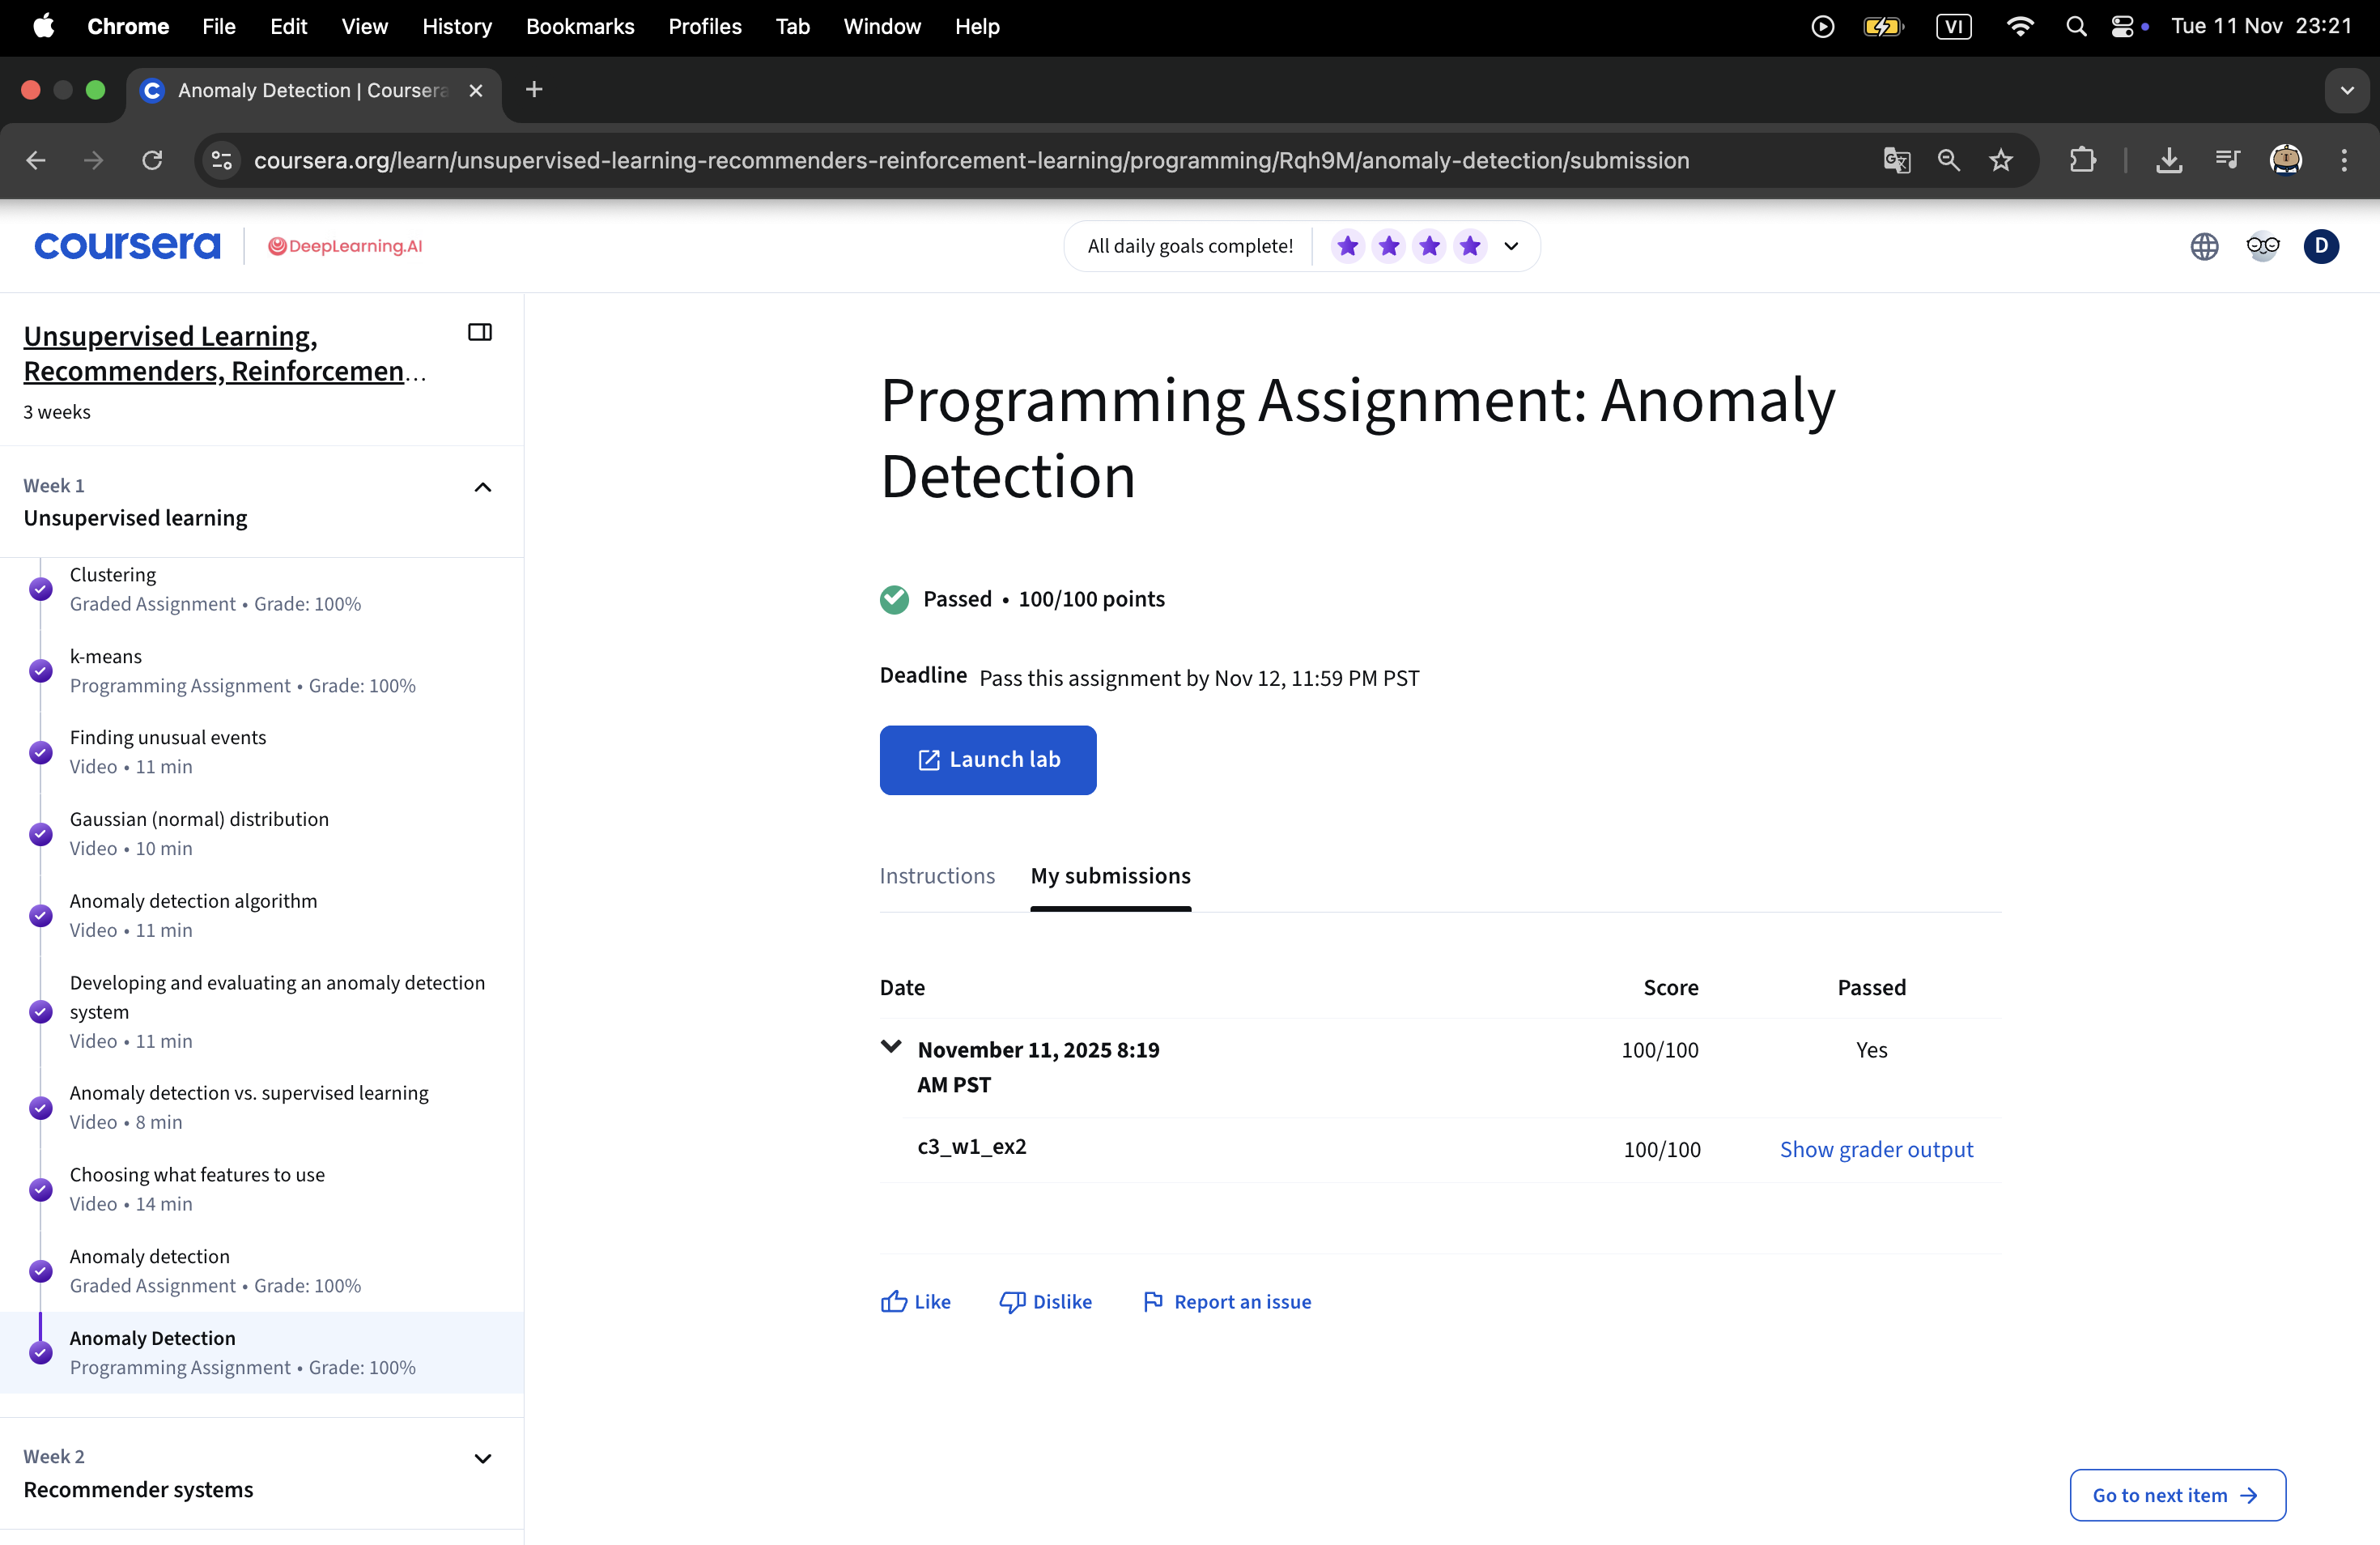
\includegraphics[scale=0.27]{Image/c3_w1_q4.png}
    \caption{Completed Programming Assignment (Anomaly Detection)}
\end{figure}

%----------------------------------------
\subsection{Week 2: Recommender Systems}
%----------------------------------------

\subsubsection{Key Insights and Learnings}

This module demystified the architecture behind modern personalization engines used by platforms like Netflix and Amazon, implementing both content-based and interaction-based approaches.

\begin{itemize}
    \item \textbf{Collaborative Filtering:} Implemented algorithms that predict user preferences based on community behavior. The model learns that users who agreed in the past will likely agree in the future, without needing explicit item attributes.
    
    \item \textbf{Content-Based Filtering:} Developed models that recommend items based on the similarity between item features (e.g., genre, keywords) and a user's profile.
    
    \item \textbf{Matrix Factorization \& Embeddings:} 
    \begin{itemize}
        \item Learned to represent users and items as vectors in a lower-dimensional space.
        \item The dot product of these vectors predicts the user rating ($y^{(i,j)} = w^{(j)} \cdot x^{(i)} + b$).
        \item Utilized \textbf{Mean Normalization} to handle the "Cold Start" problem for new users with no history.
    \end{itemize}
\end{itemize}

\subsubsection{Learning Evidence}
\begin{figure}[H]
    \centering
    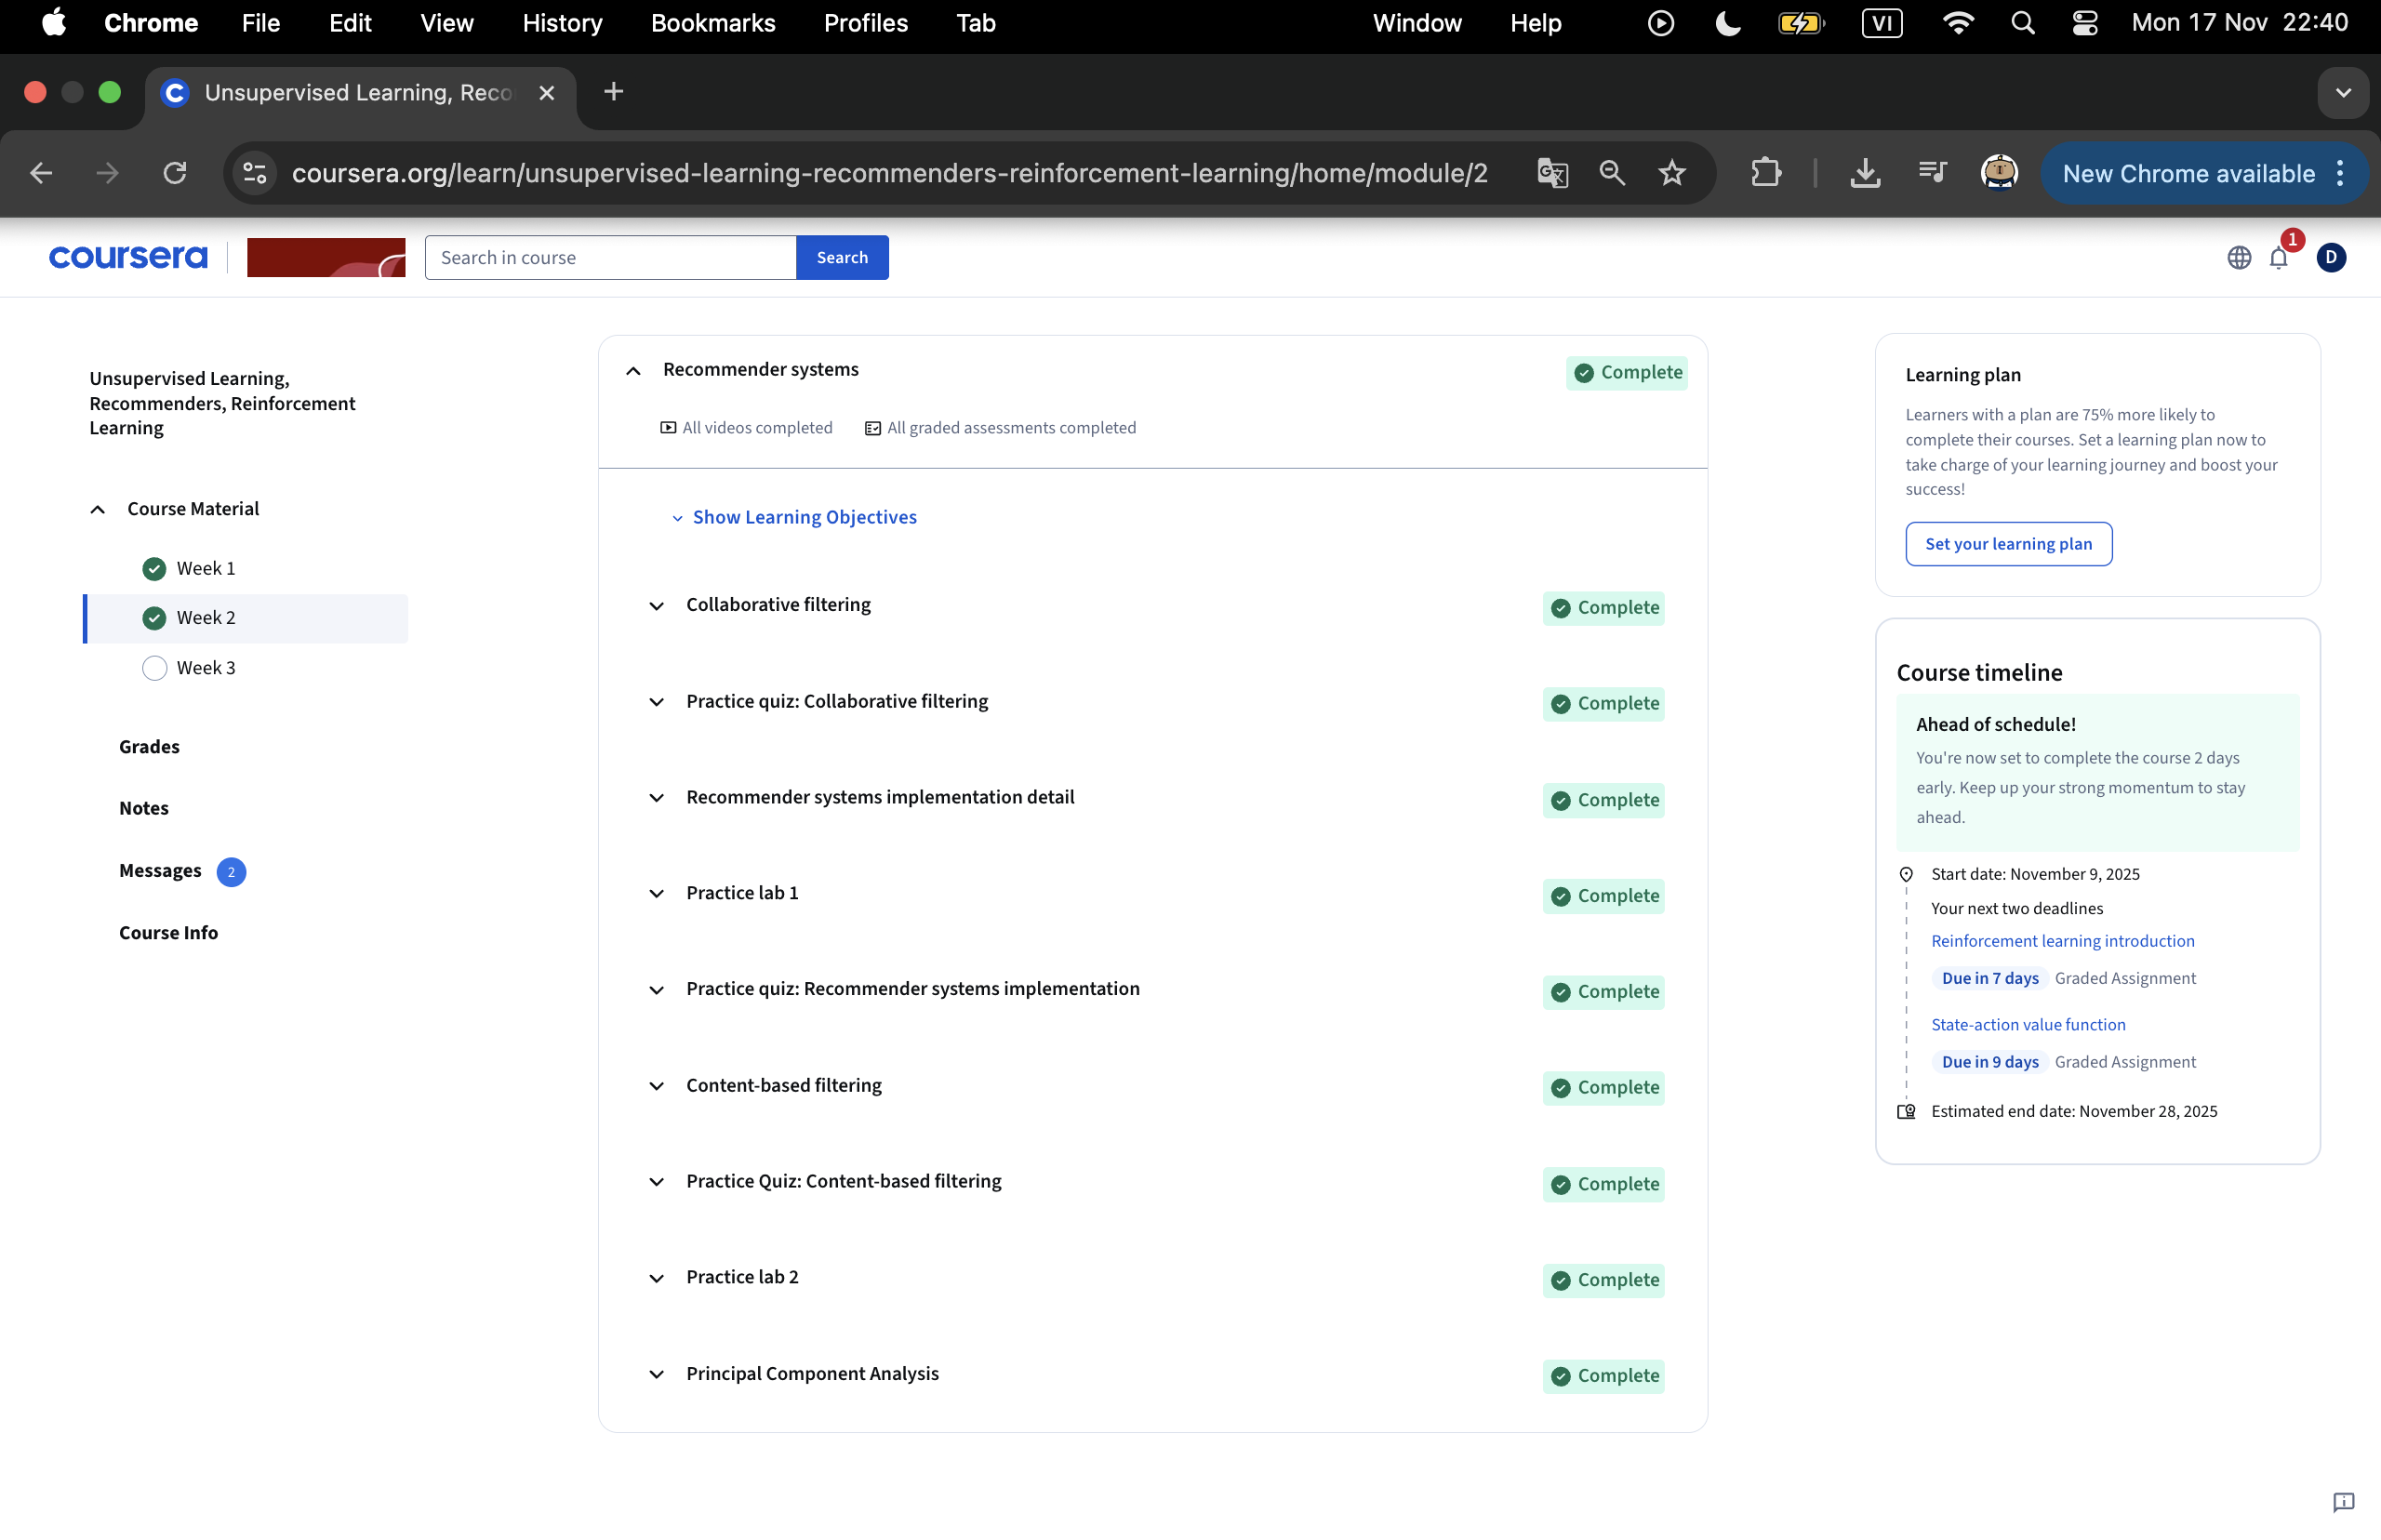
\includegraphics[scale=0.35]{Image/c3_w2.png}
    \caption{Lesson's completed date (17/11/2025)}
\end{figure}

\subsubsection{Graded Assignment Evidence}
\begin{figure}[H]
    \centering
    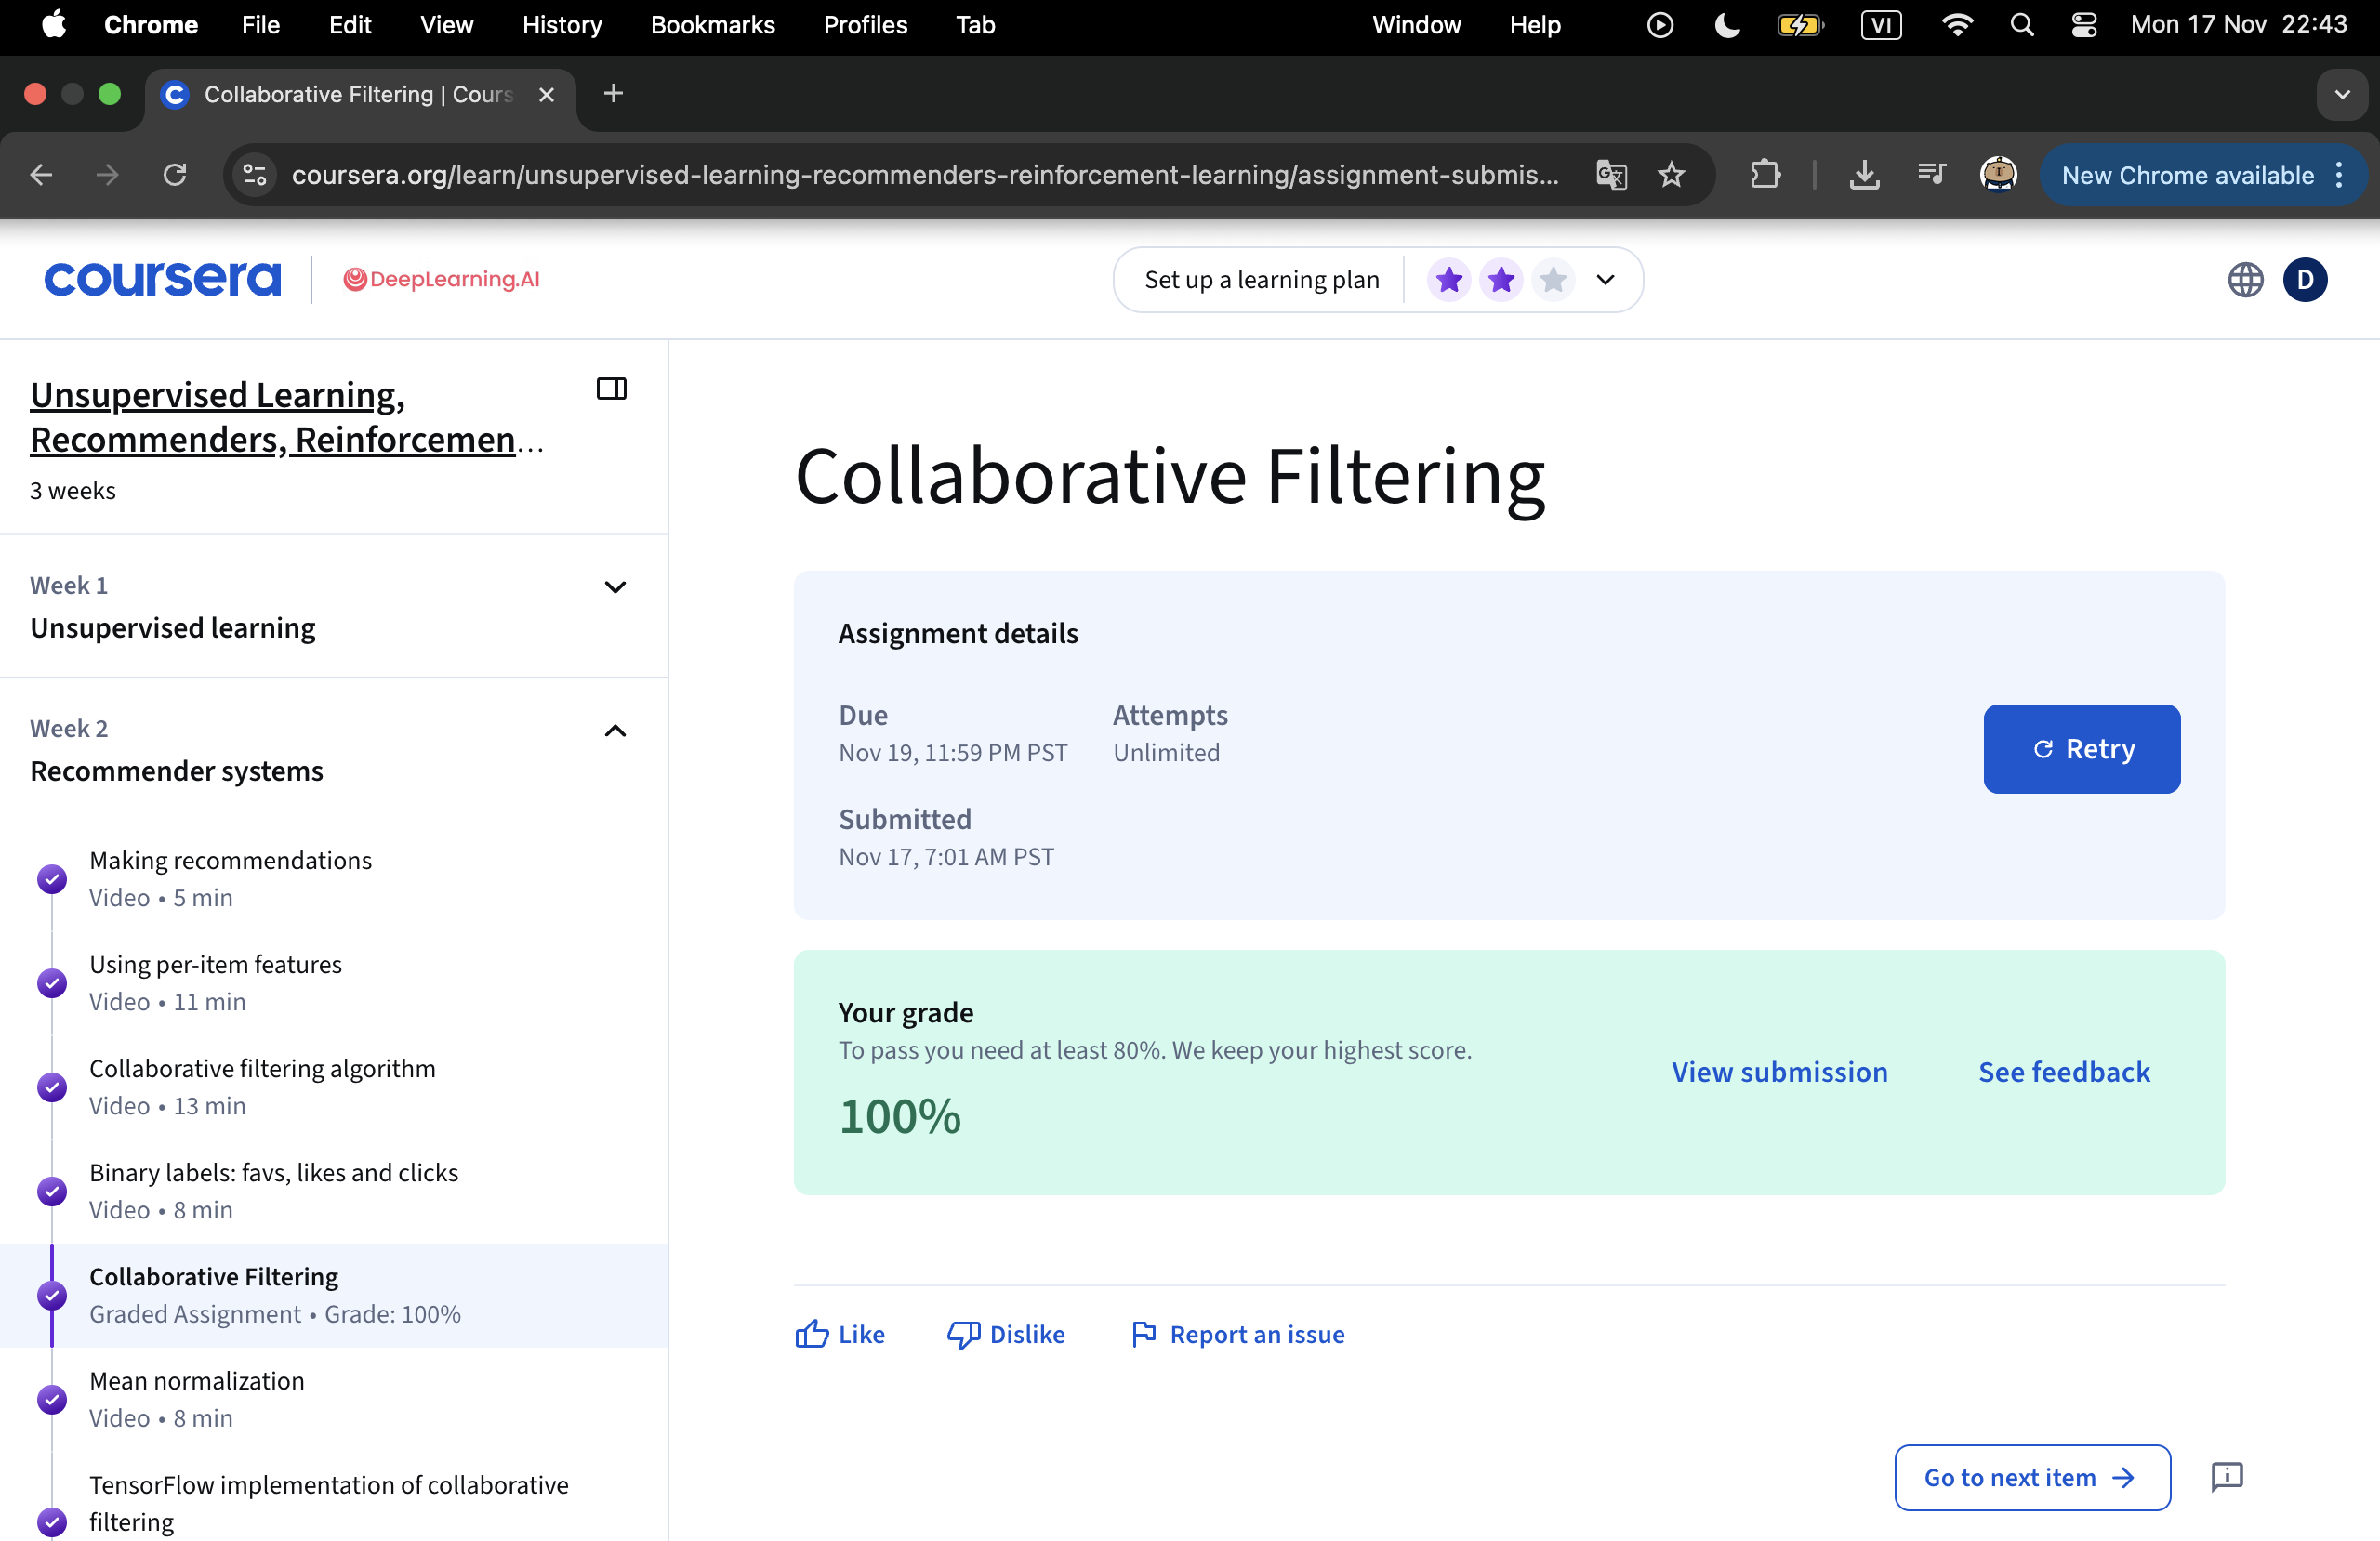
\includegraphics[scale=0.27]{Image/c3_w2_q1.png}
    \caption{Completed Graded Assignment 1 (Collaborative Filtering)}
\end{figure}

\begin{figure}[H]
    \centering
    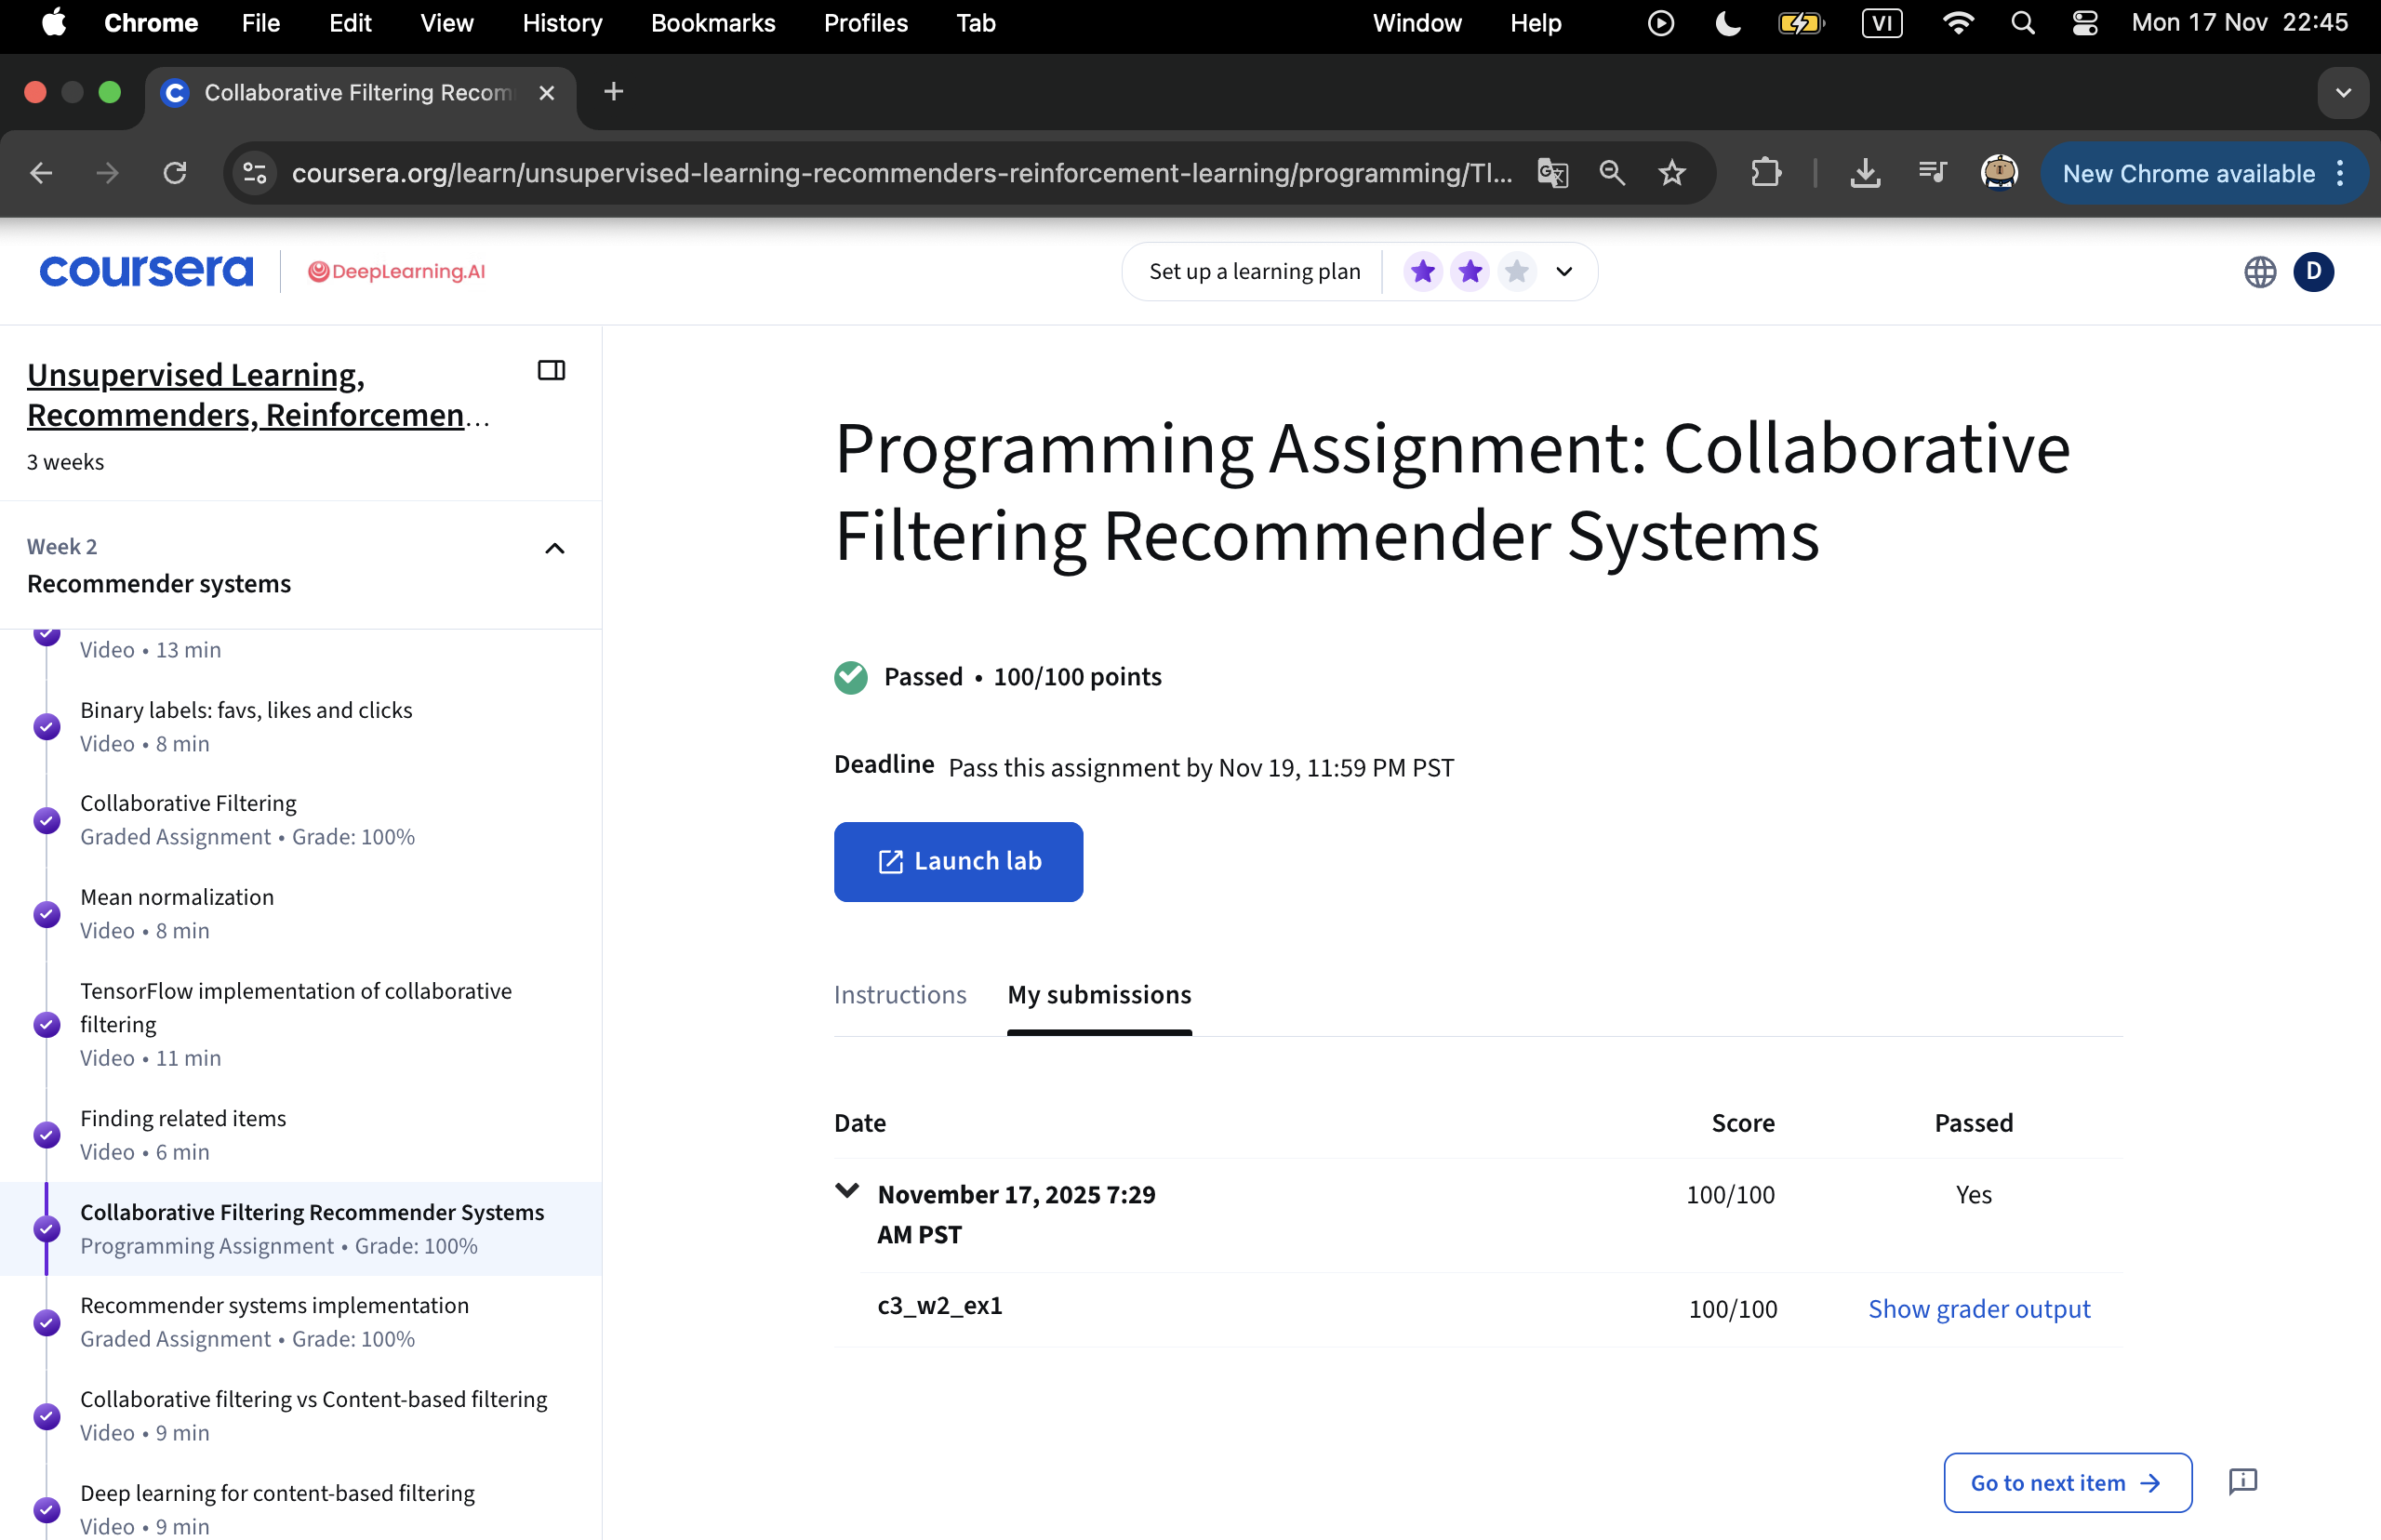
\includegraphics[scale=0.27]{Image/c3_w2_q2.png}
    \caption{Completed Programming Assignment (Collaborative Filtering Recommender Systems)}
\end{figure}

\begin{figure}[H]
    \centering
    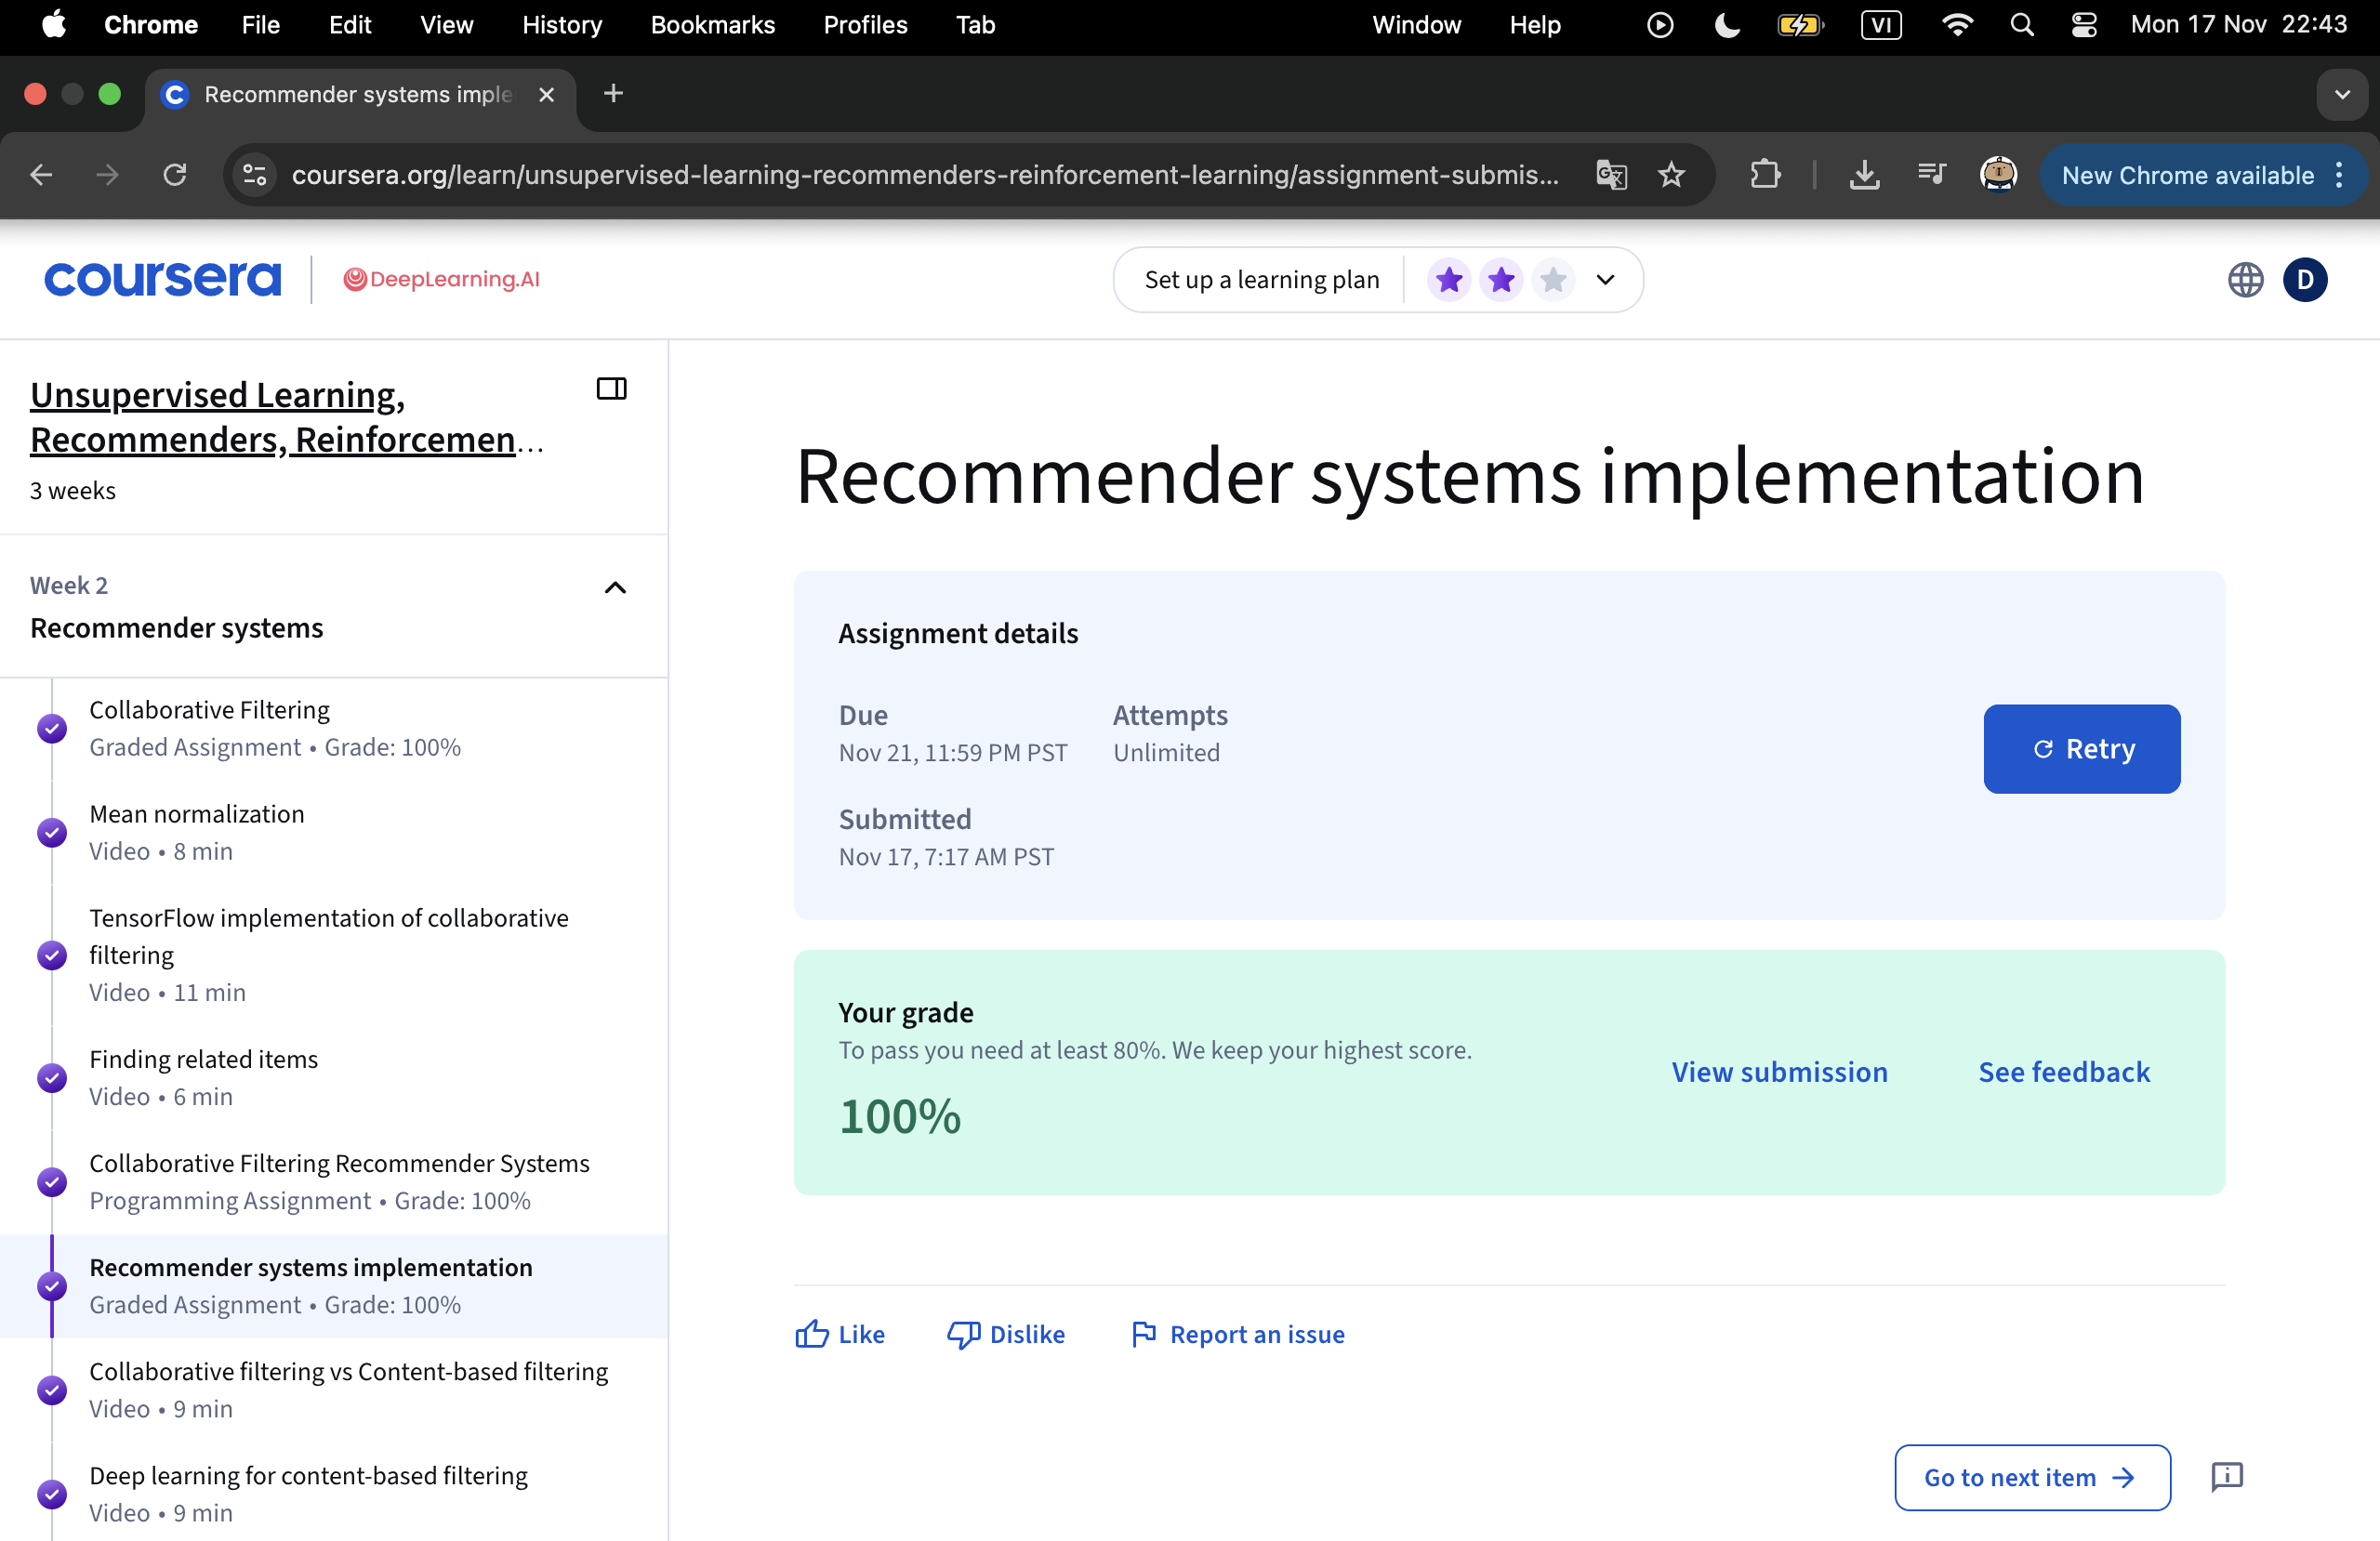
\includegraphics[scale=0.27]{Image/c3_w2_q3.png}
    \caption{Completed Graded Assignment 3 (Recommender systems implementation)}
\end{figure}

\begin{figure}[H]
    \centering
    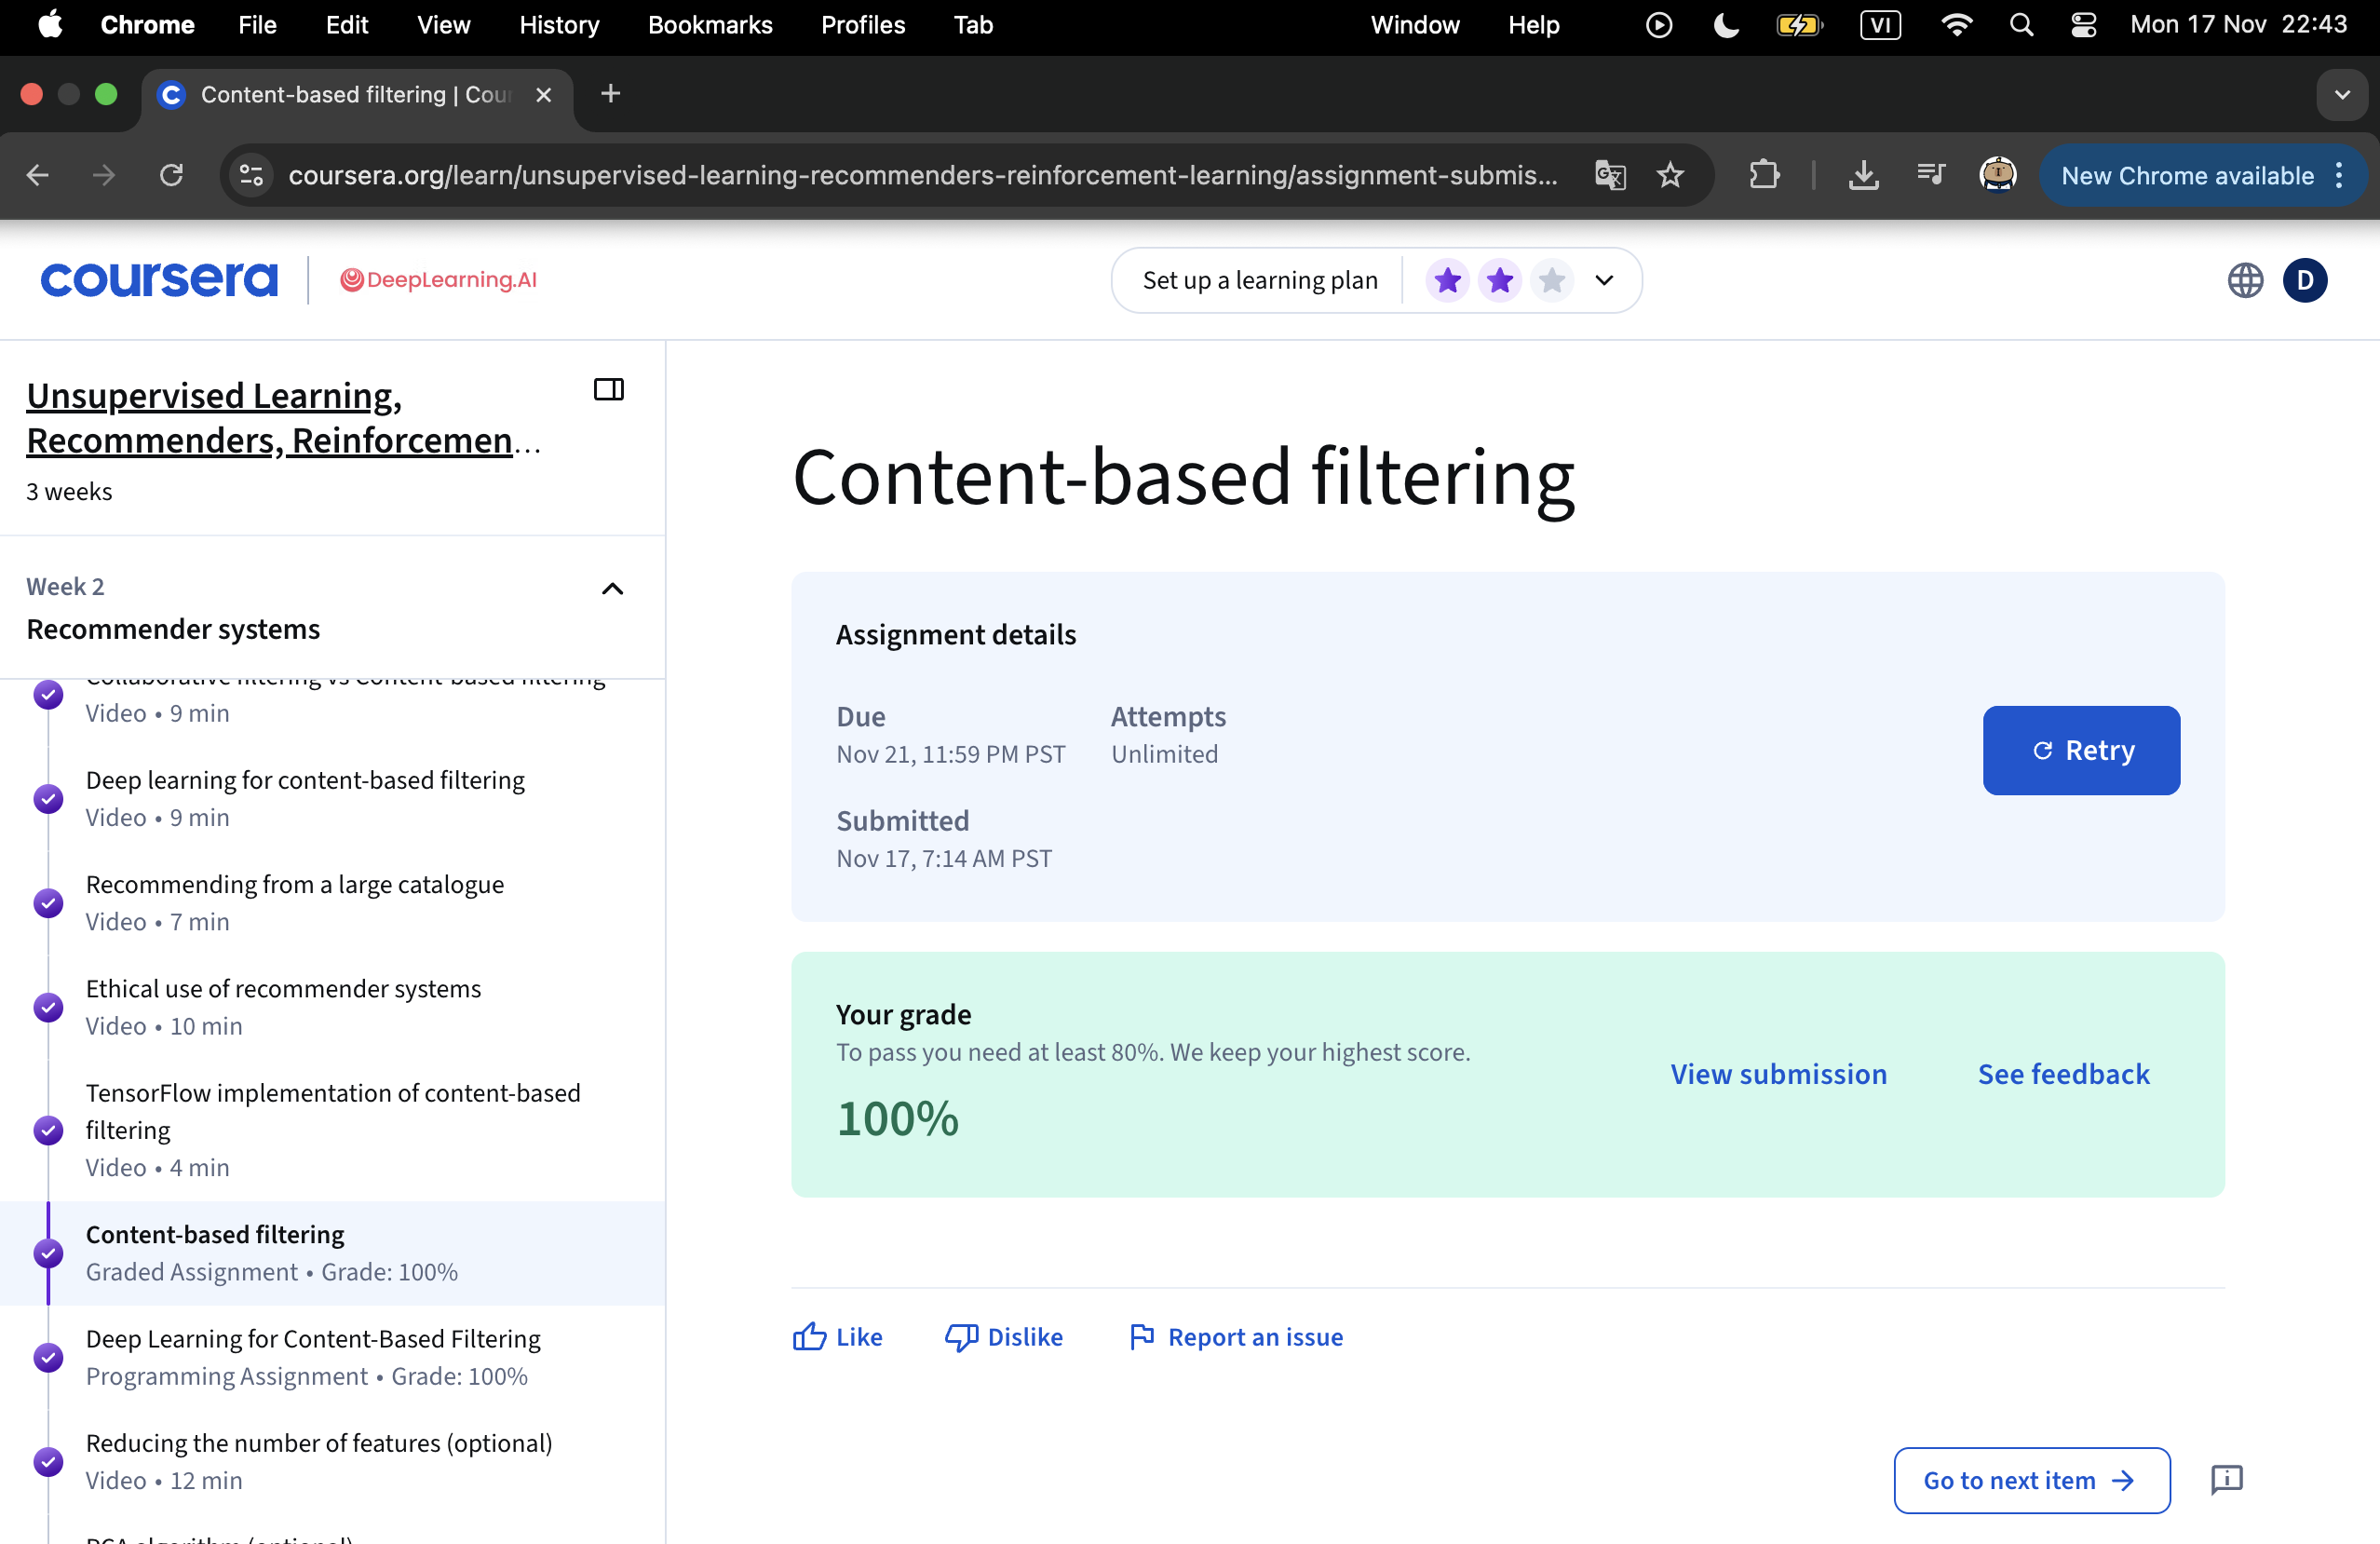
\includegraphics[scale=0.27]{Image/c3_w2_q4.png}
    \caption{Completed Graded Assignment 3 (Content-based filtering)}
\end{figure}

\begin{figure}[H]
    \centering
    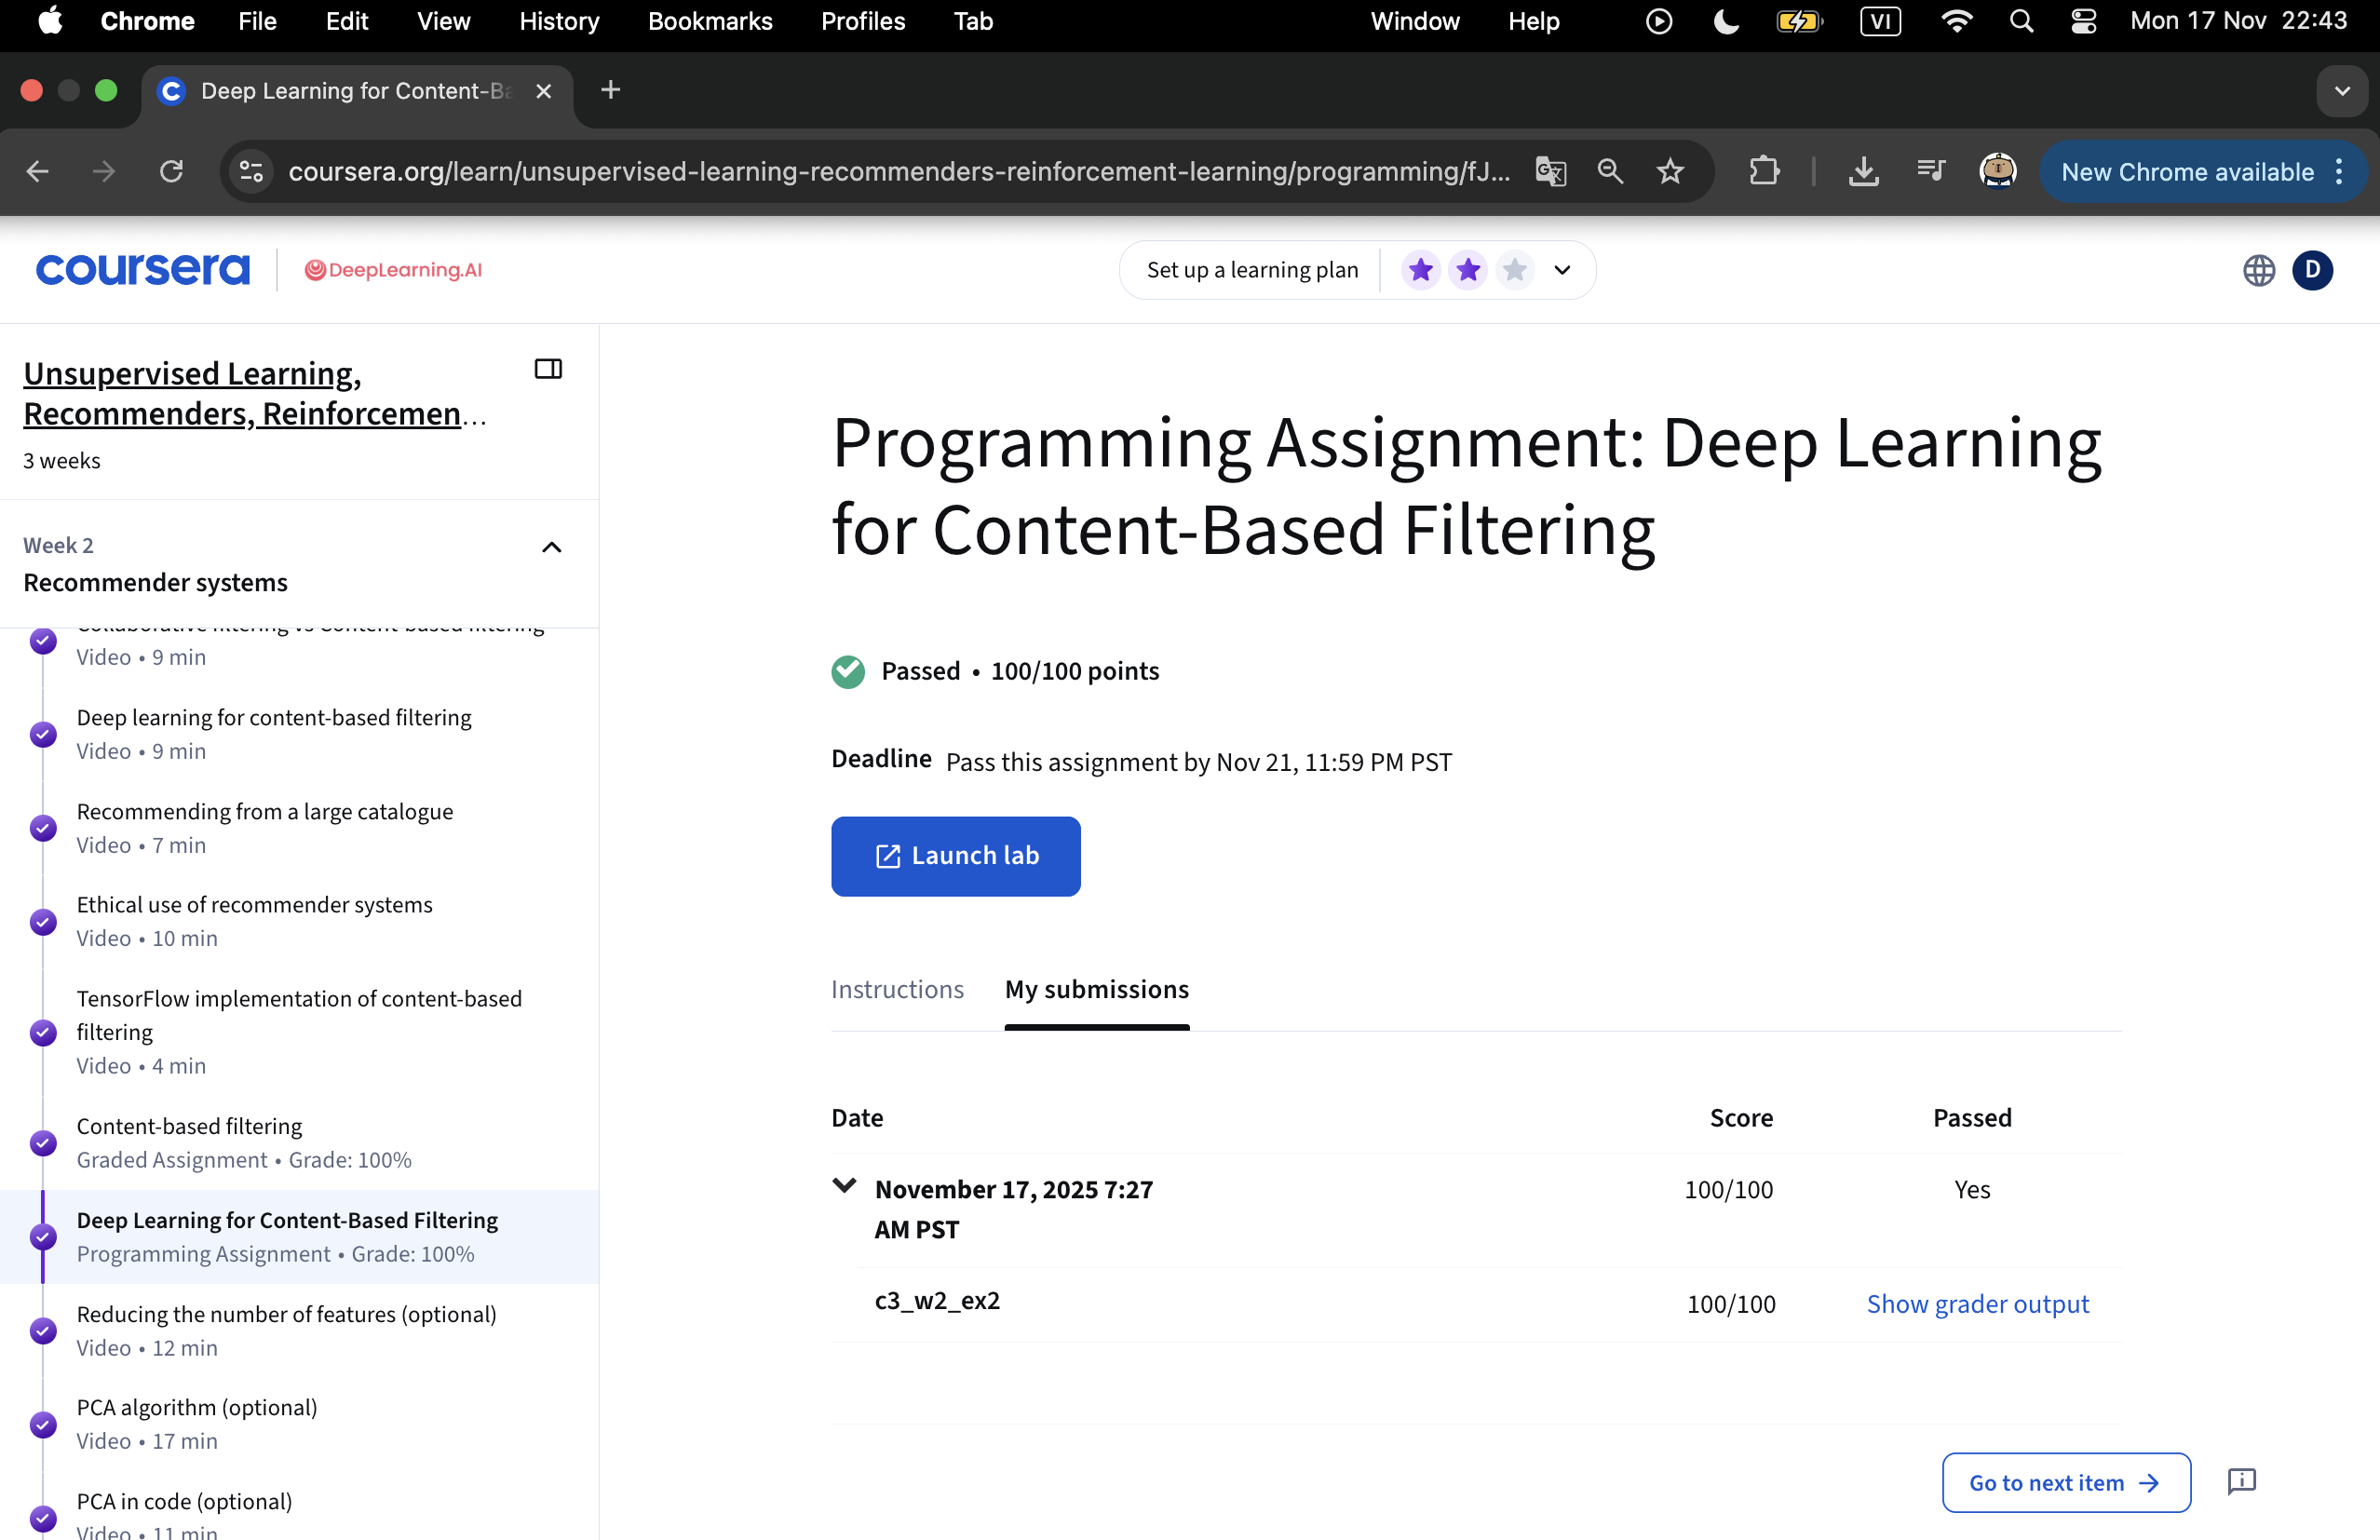
\includegraphics[scale=0.27]{Image/c3_w2_q5.png}
    \caption{Completed Programming Assignment (Deep Learning for Content-Based Filtering)}
\end{figure}


%----------------------------------------
\subsection{Week 3: Reinforcement Learning (RL)}
%----------------------------------------

\subsubsection{Key Insights and Learnings}

This module introduced a paradigm shift where an agent learns a policy to maximize rewards over time, rather than minimizing instantaneous error.

\begin{itemize}
    \item \textbf{The RL Framework (MDP):} Defined the problem as a Markov Decision Process, consisting of States ($S$), Actions ($A$), Rewards ($R$), and a Discount factor ($\gamma$). The goal is to maximize the expected \textit{Return}.
    
    \item \textbf{The Bellman Equation:} Understood the recursive relationship that defines the value of a state-action pair. This equation is the foundation for updating the Q-function to estimate long-term rewards.
    
    \item \textbf{Deep Q-Learning (DQN):} 
    \begin{itemize}
        \item Replaced traditional Q-tables with Neural Networks to approximate the Q-function, enabling the agent to handle complex, high-dimensional state spaces (e.g., video game pixels or robot sensors).
        \item \textbf{Exploration vs. Exploitation:} Implemented the $\epsilon$-greedy policy to balance trying new actions versus leveraging known optimal actions.
    \end{itemize}
\end{itemize}

\subsubsection{Learning Evidence}
\begin{figure}[H]
    \centering
    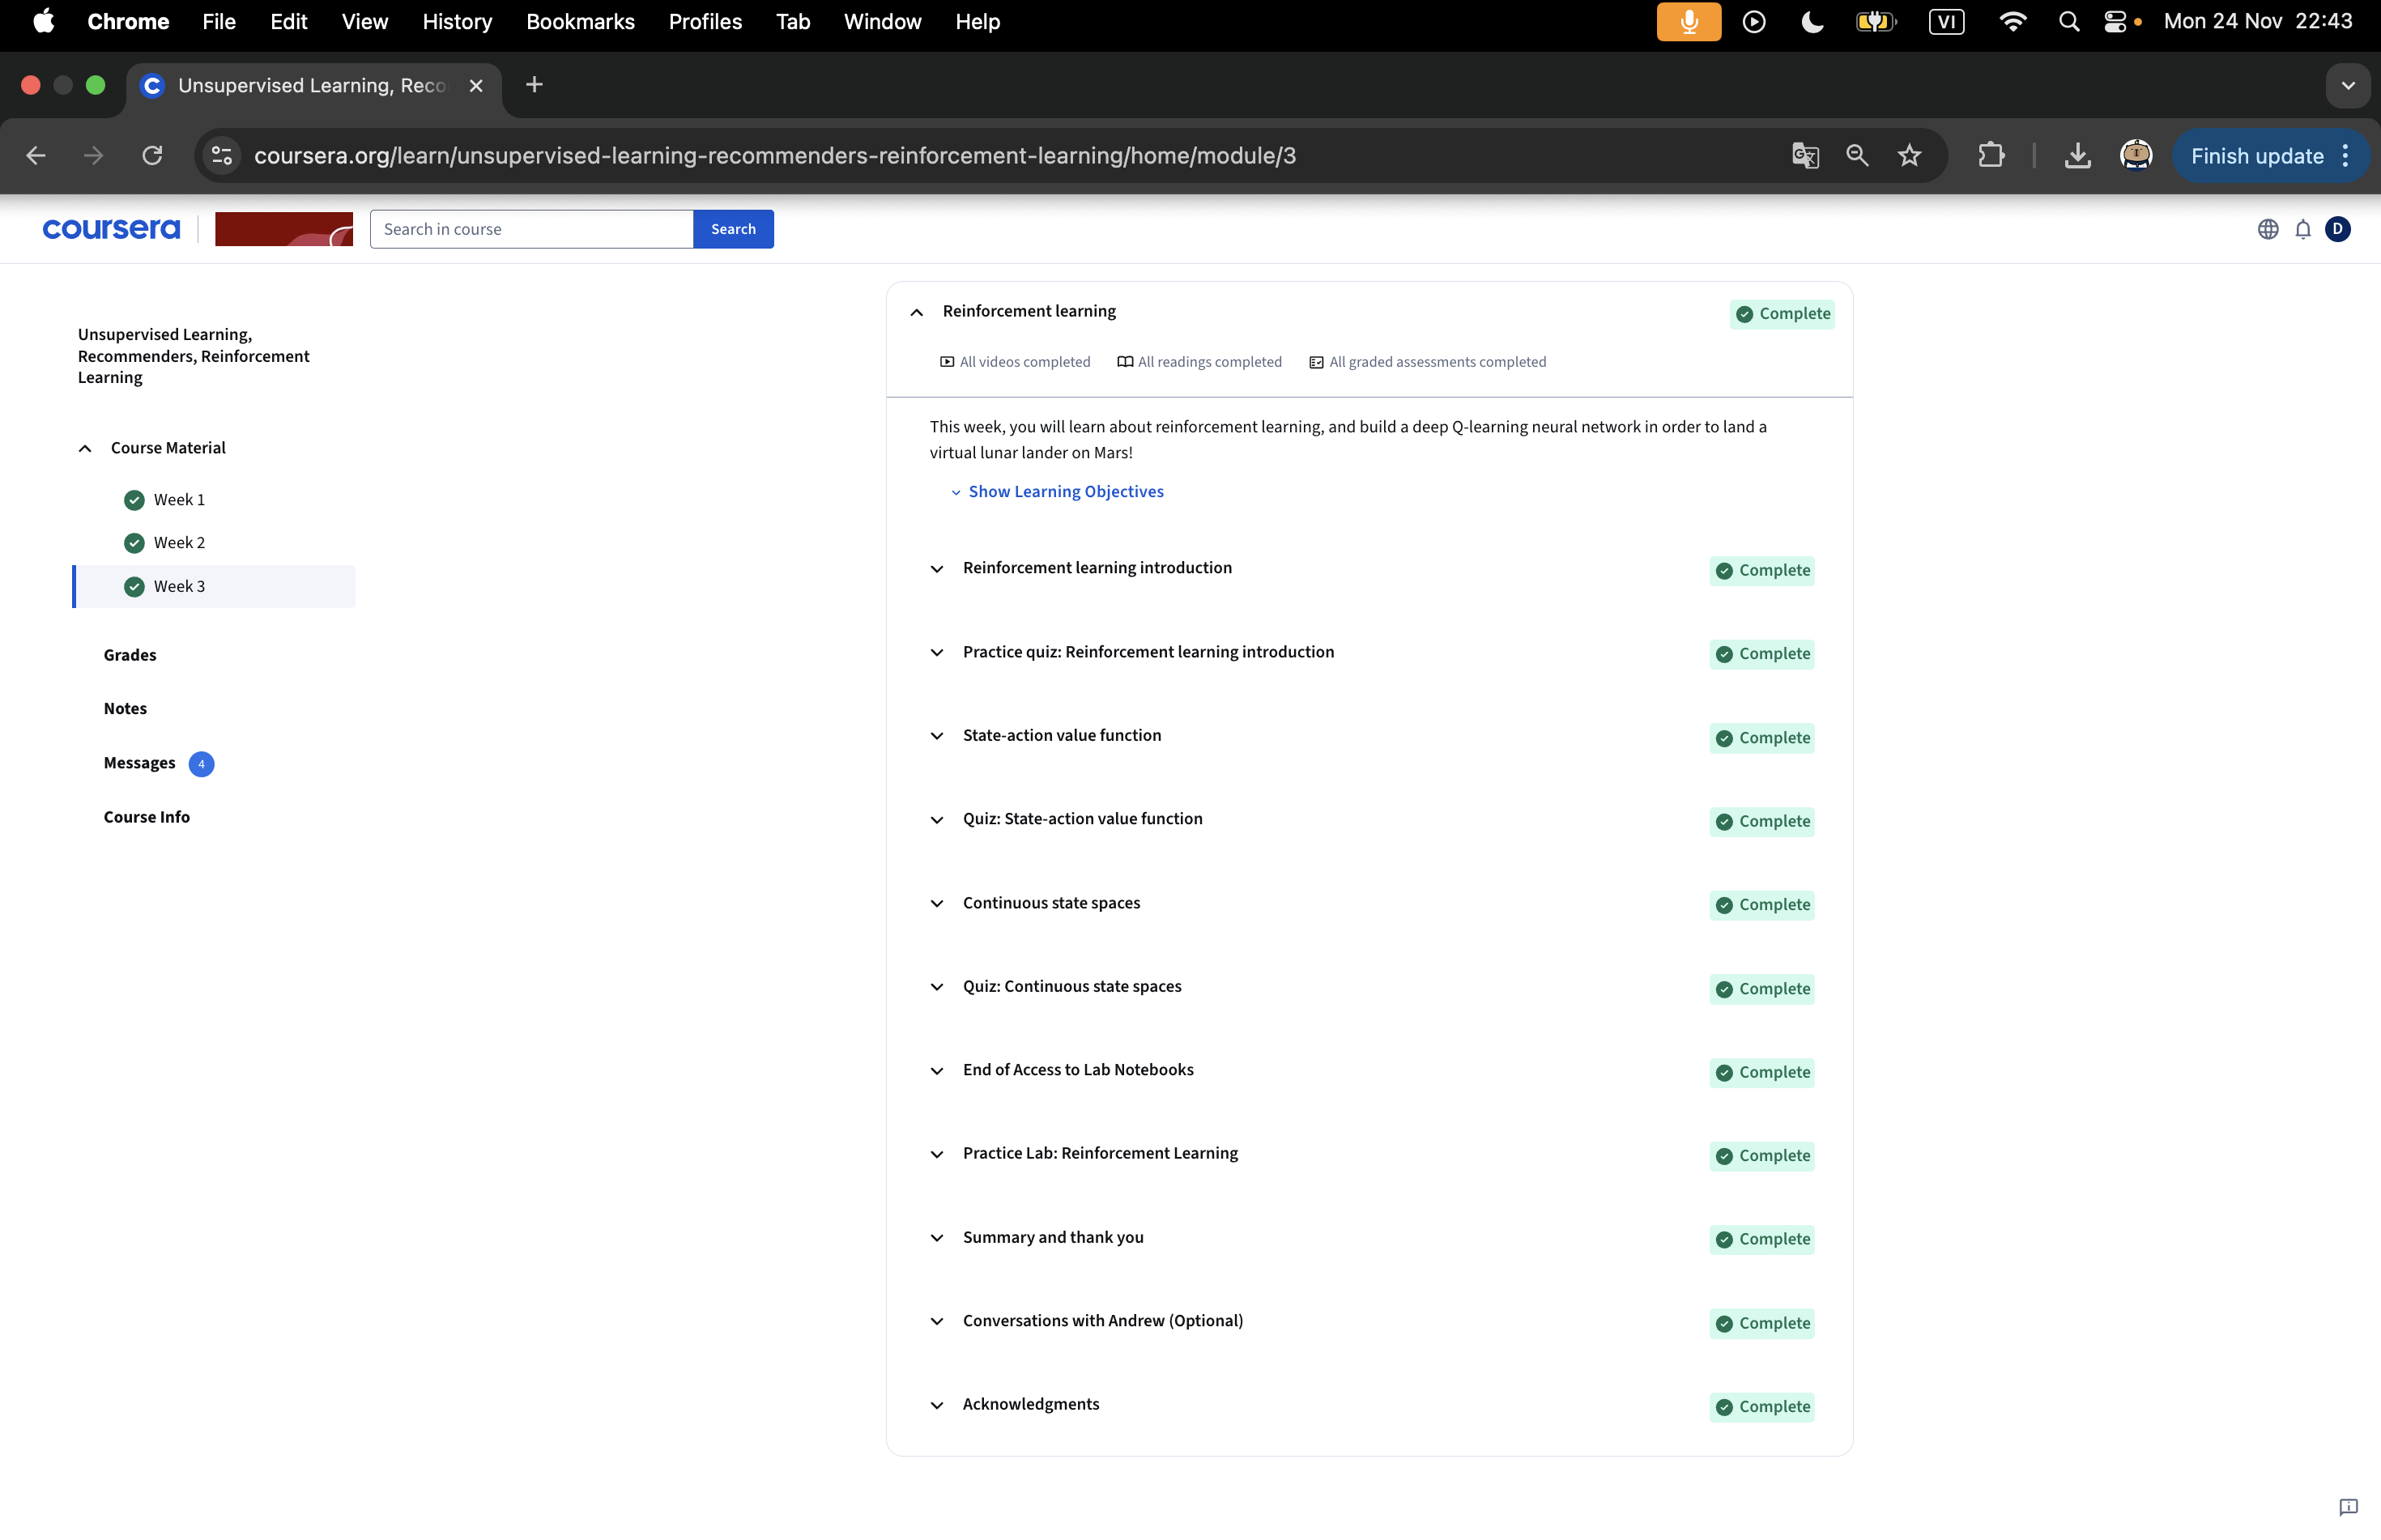
\includegraphics[scale=0.25]{Image/c3_w3.png}
    \caption{Lesson's completed date (24/11/2025)}
\end{figure}

\subsubsection{Graded Assignment Evidence}
\begin{figure}[H]
    \centering
    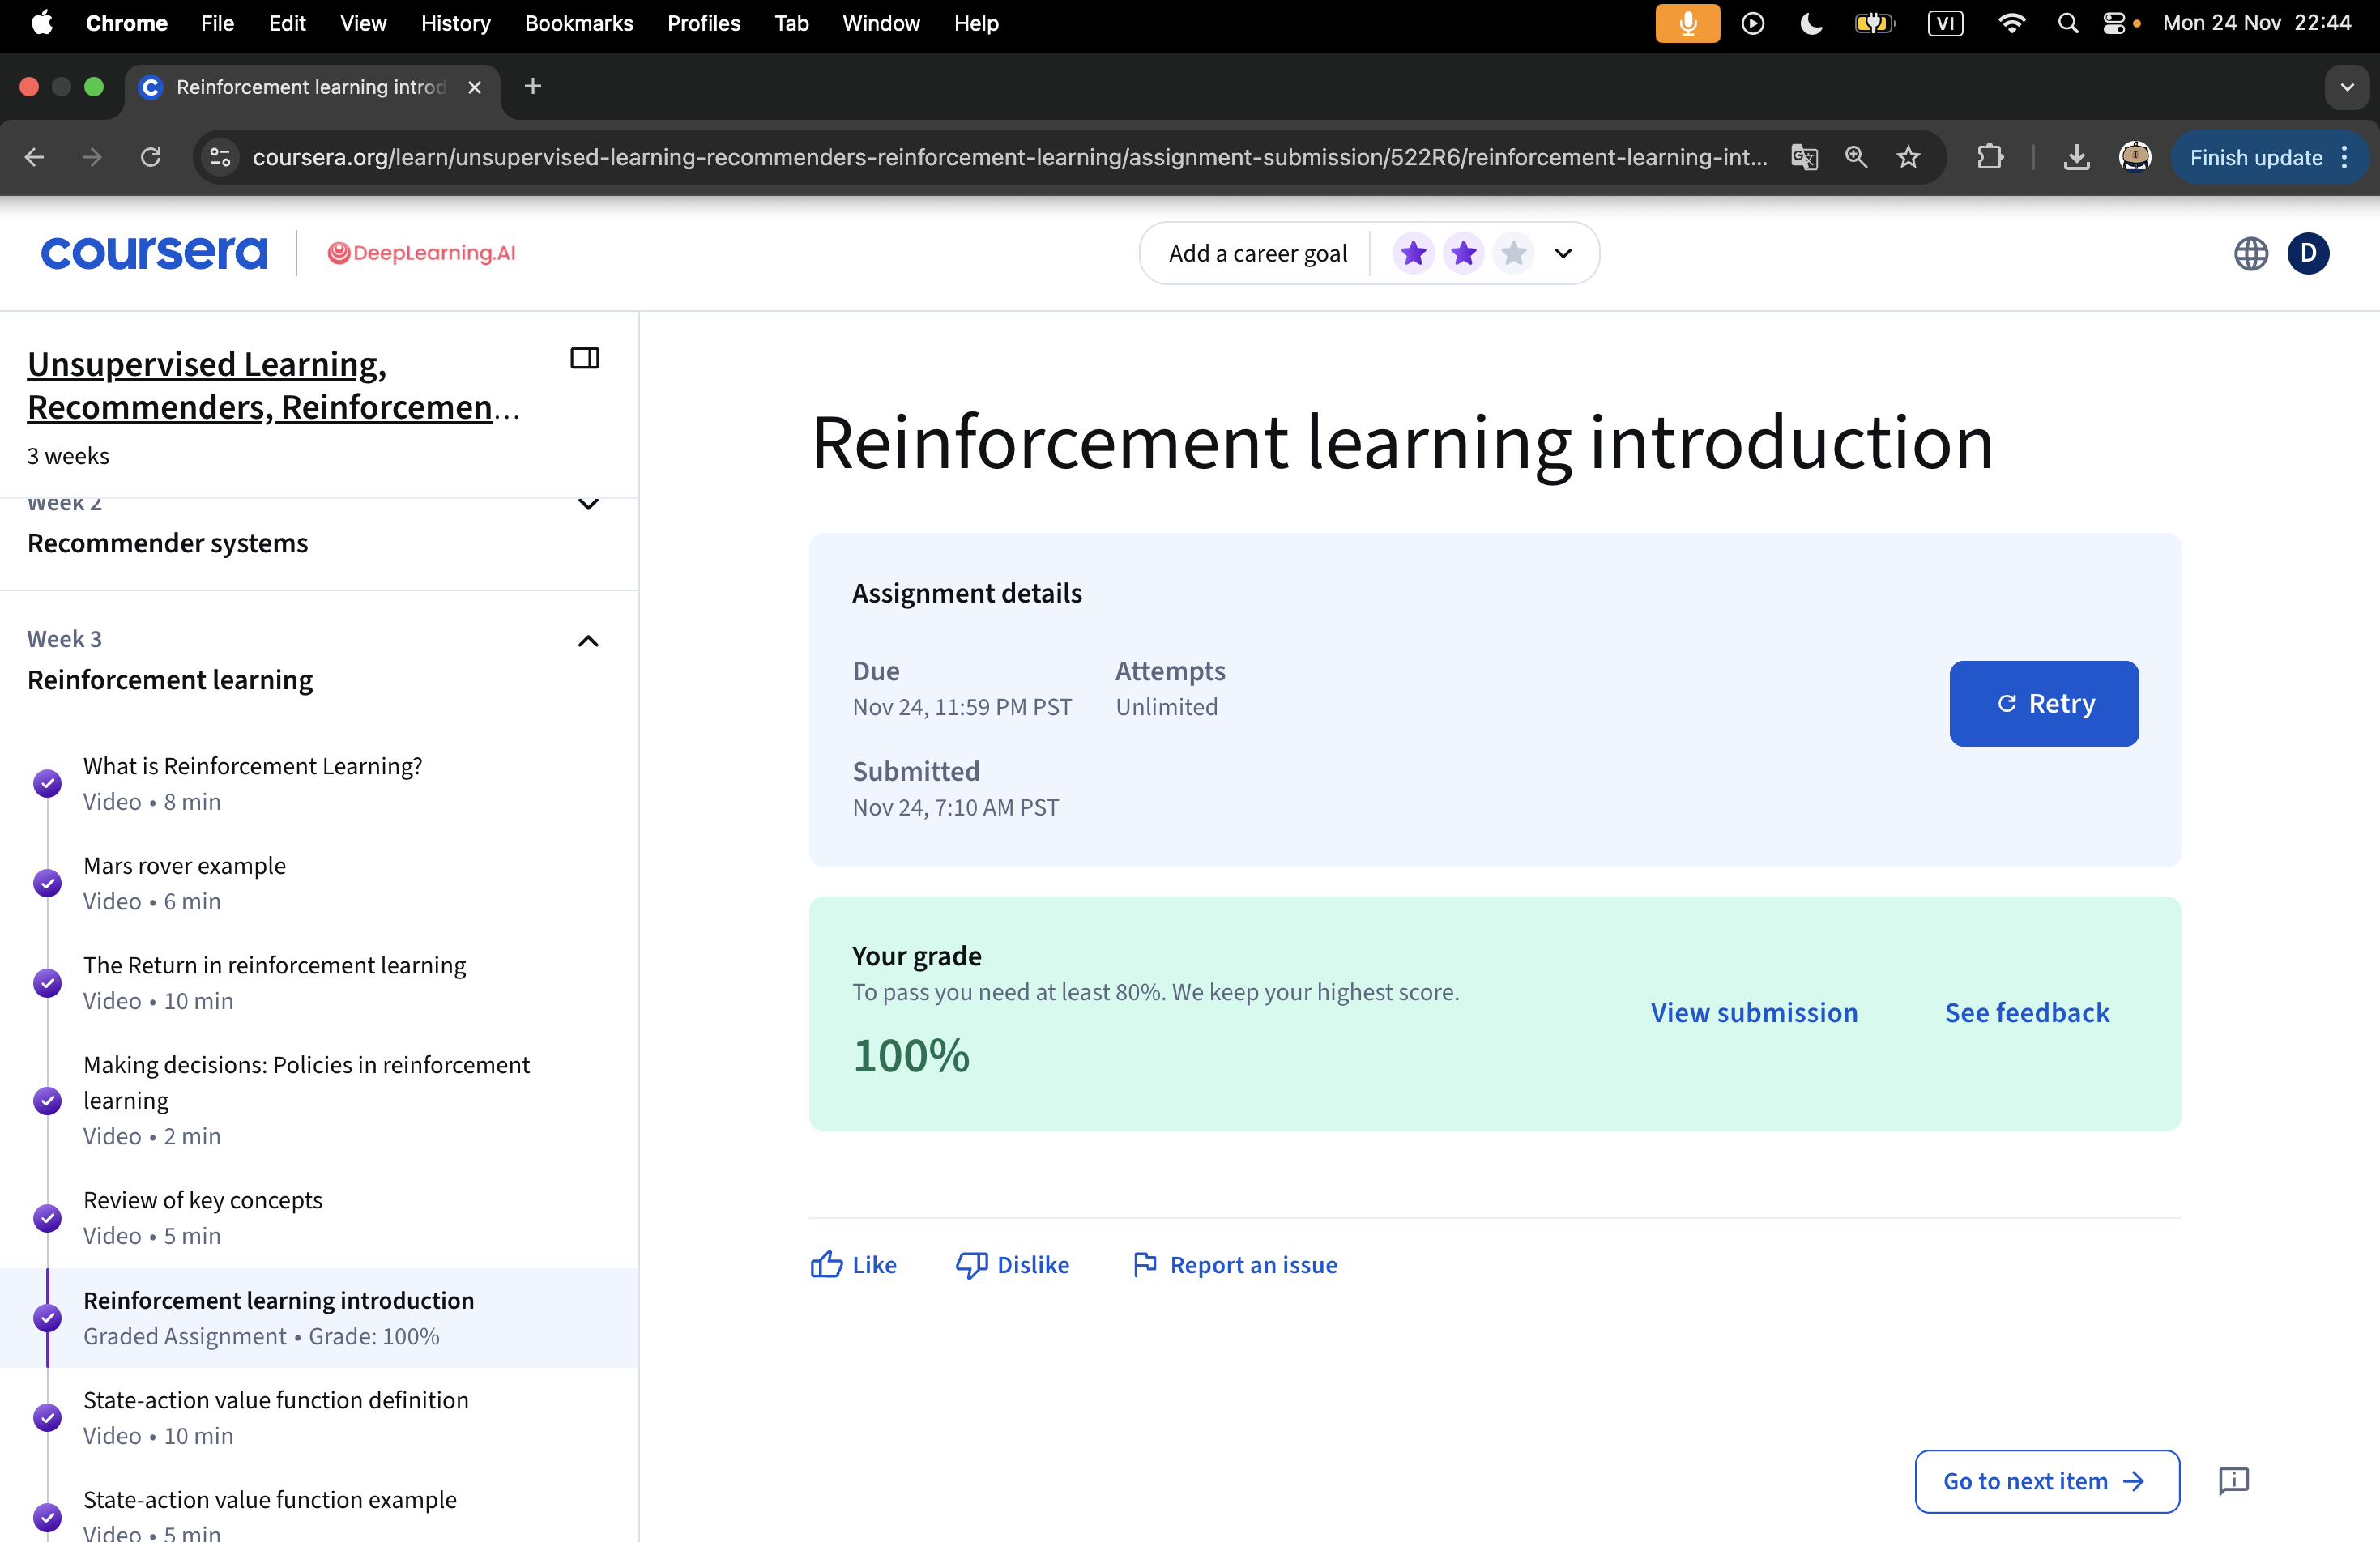
\includegraphics[scale=0.25]{Image/c3_w3_q1.png}
    \caption{Completed Graded Assignment 1 (Reinforcement learning introduction)}
\end{figure}

\begin{figure}[H]
    \centering
    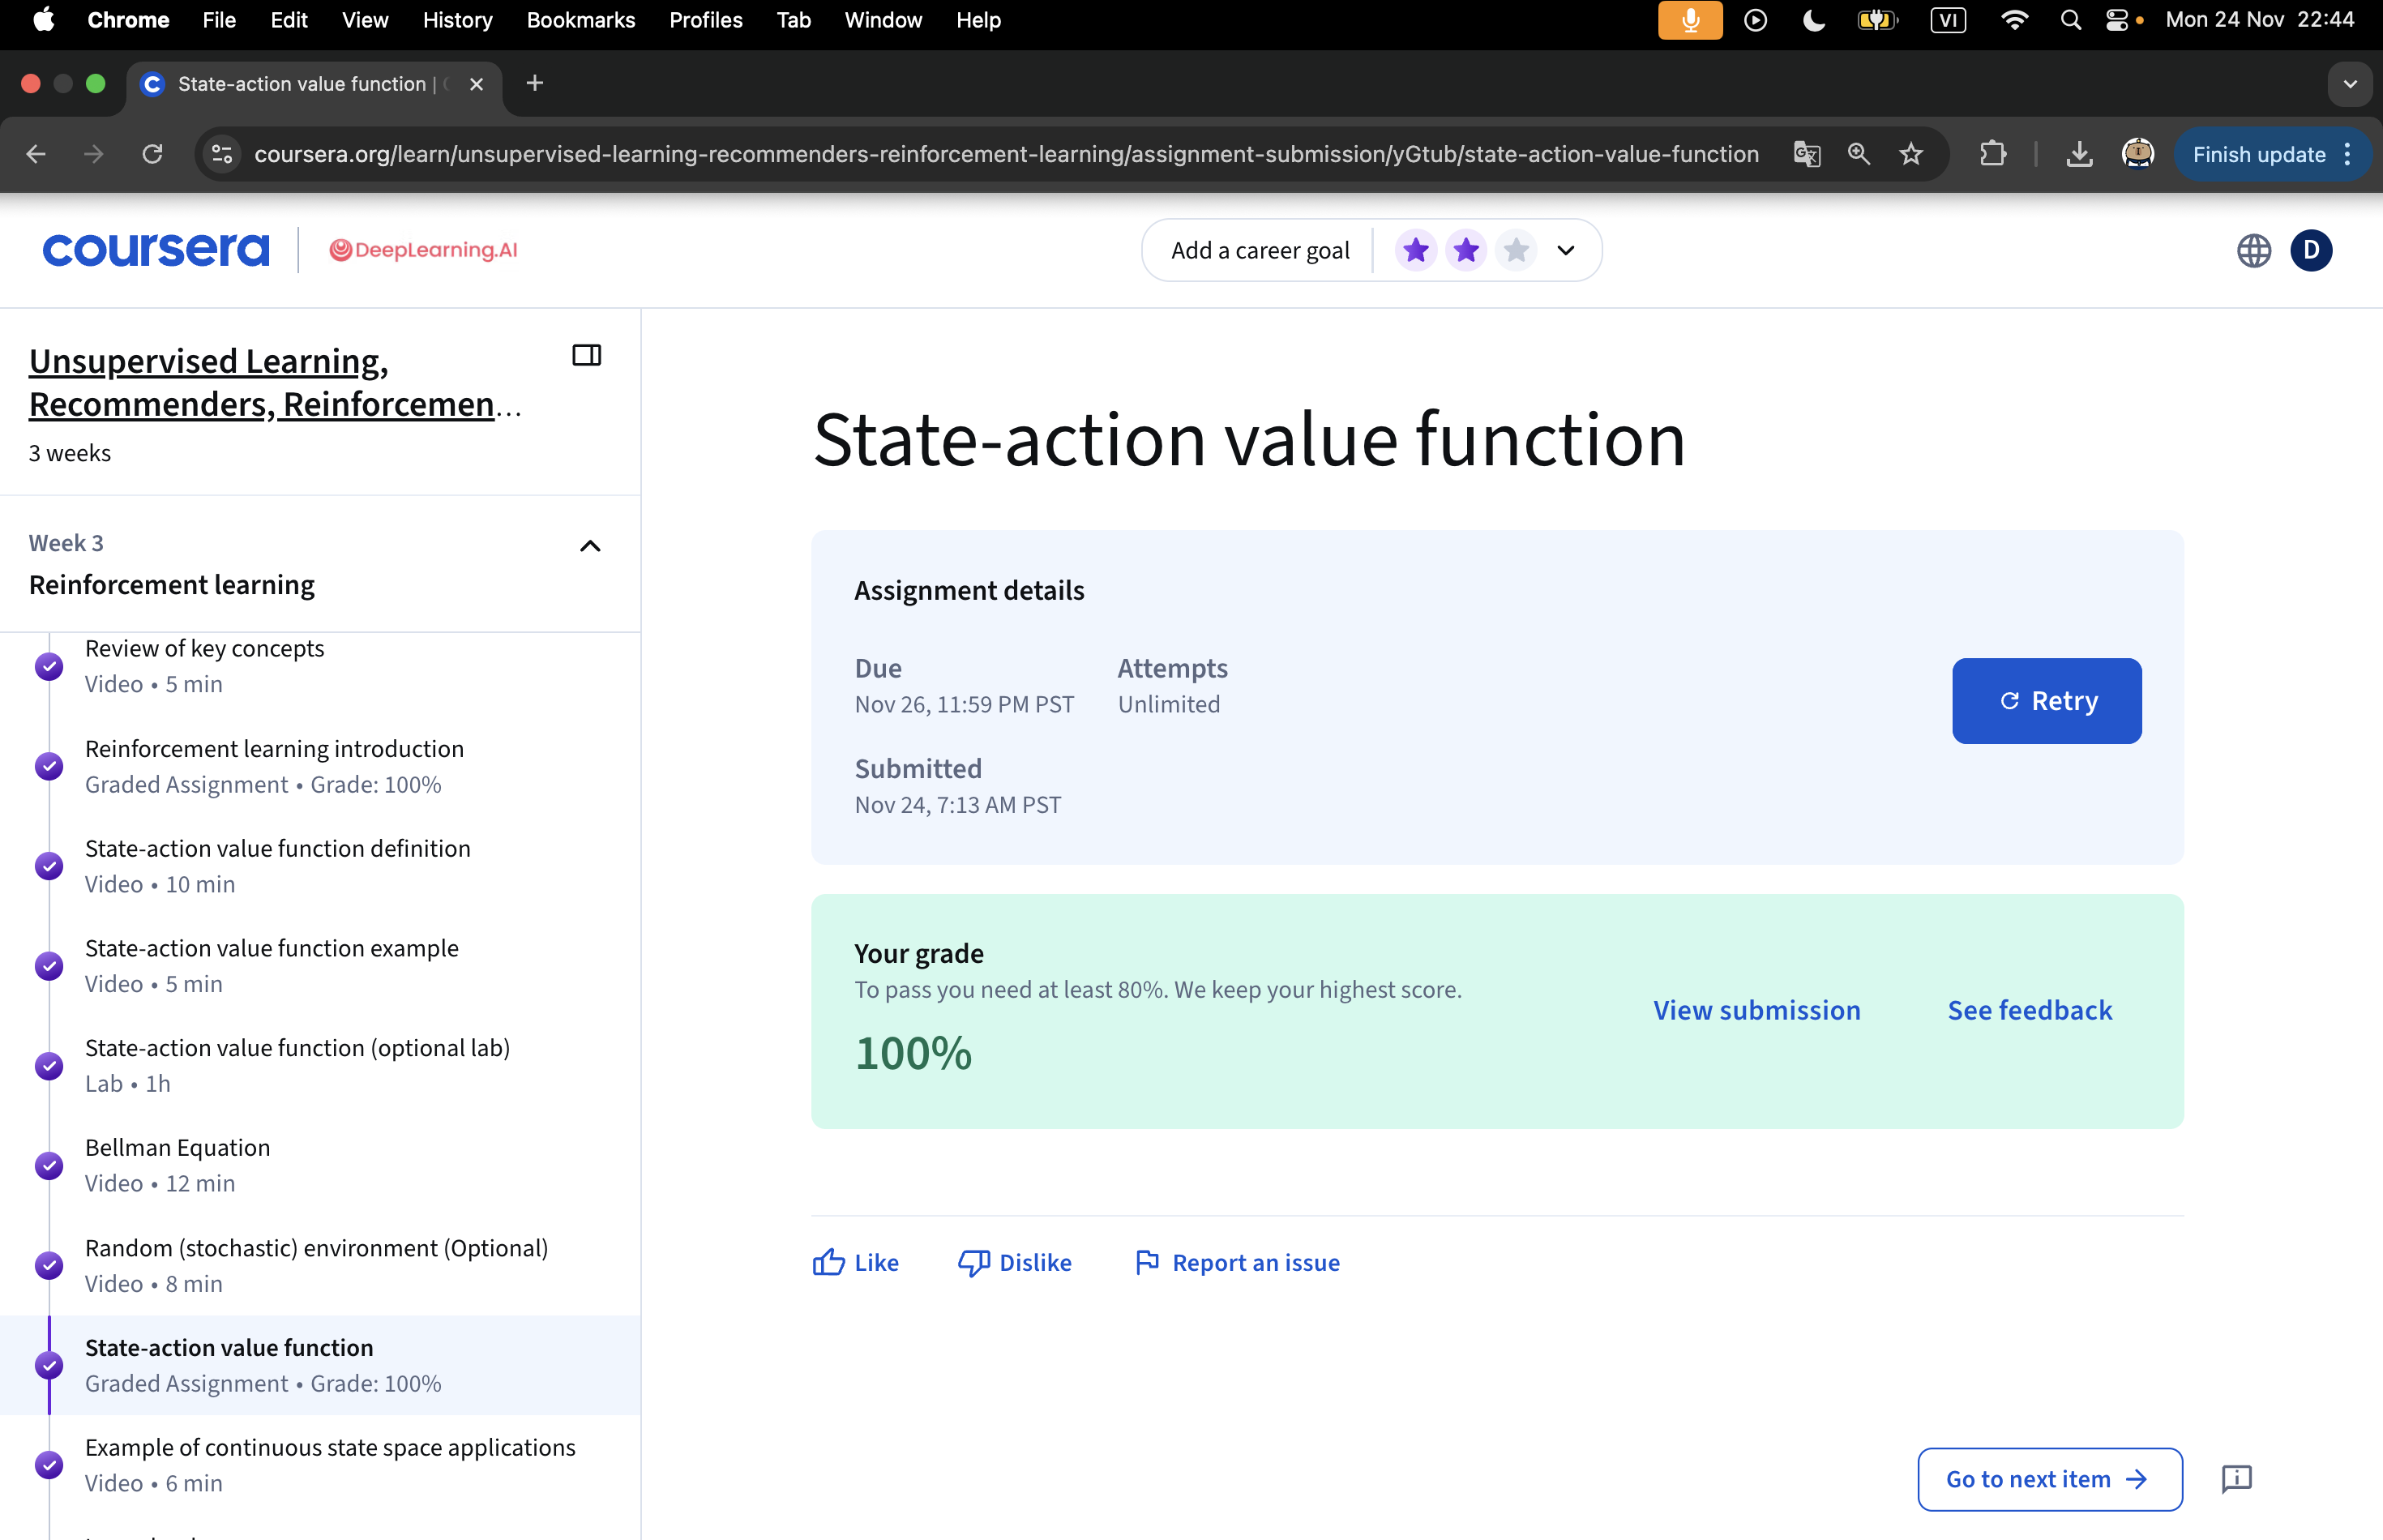
\includegraphics[scale=0.25]{Image/c3_w3_q2.png}
    \caption{Completed Graded Assignment 2 (State-action value function)}
\end{figure}

\begin{figure}[H]
    \centering
    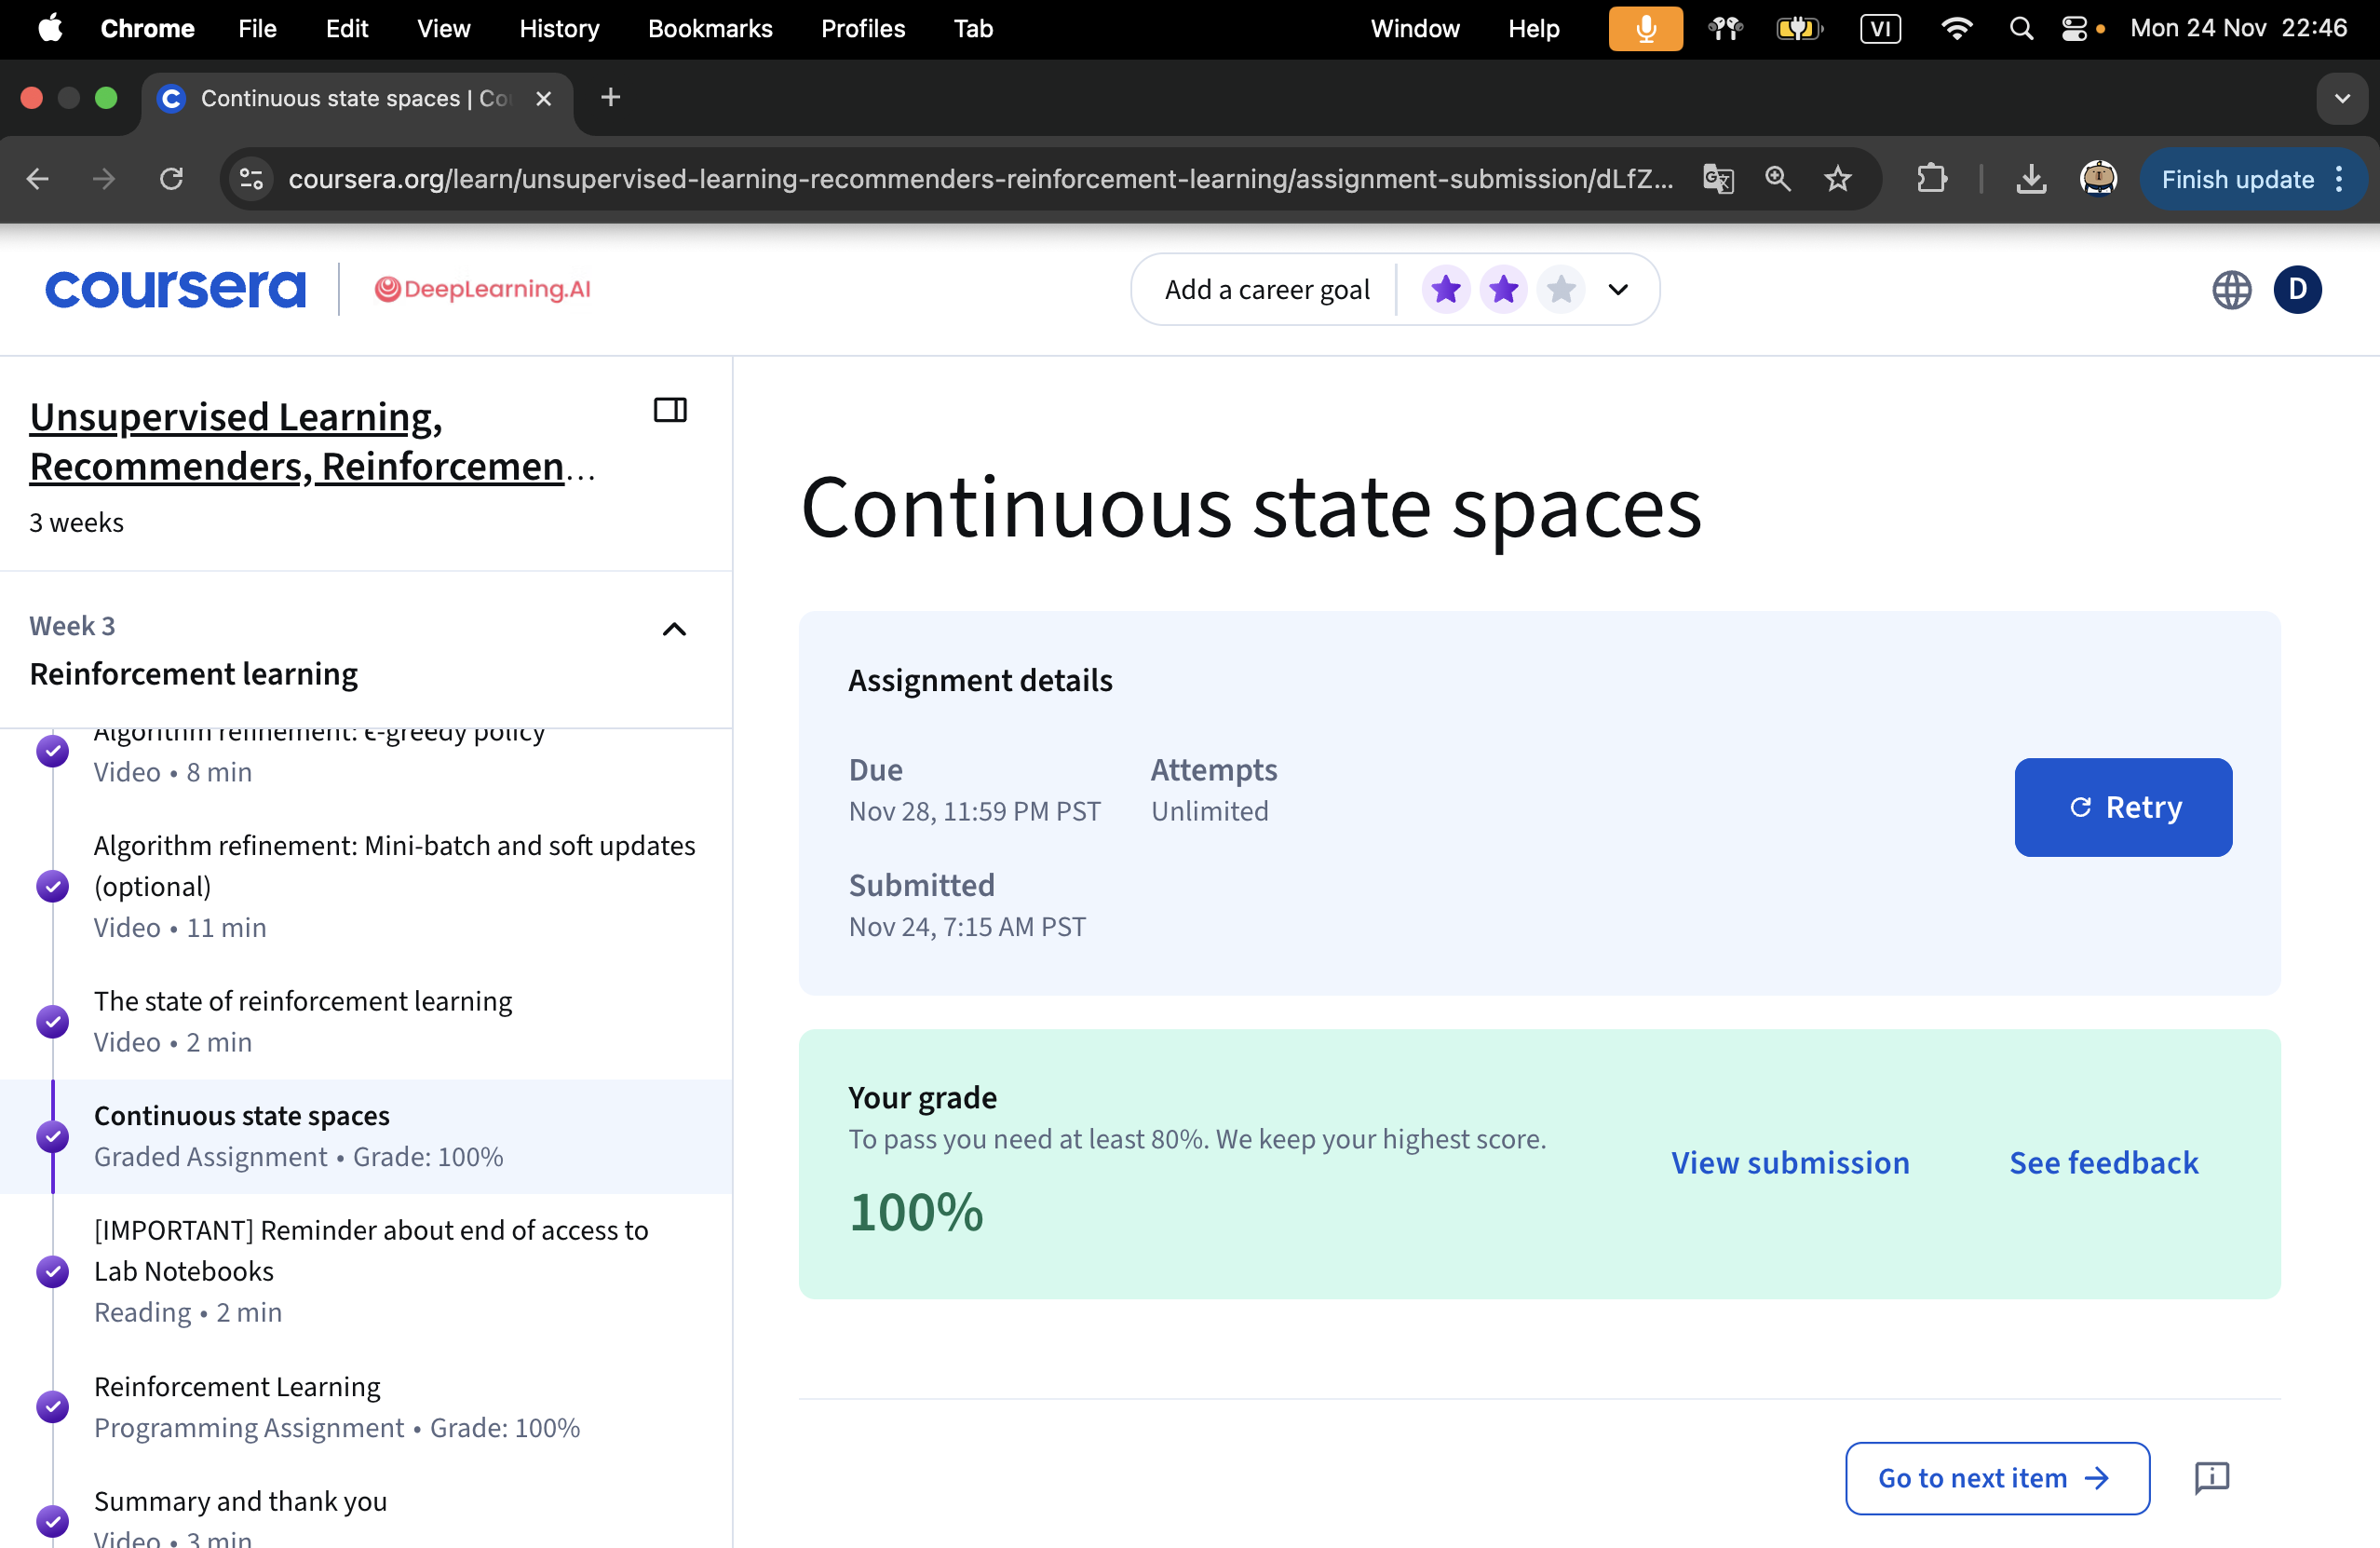
\includegraphics[scale=0.25]{Image/c3_w3_q3.png}
    \caption{Completed Graded Assignment 3 (Continuous state spaces)}
\end{figure}


\begin{figure}[H]
    \centering
    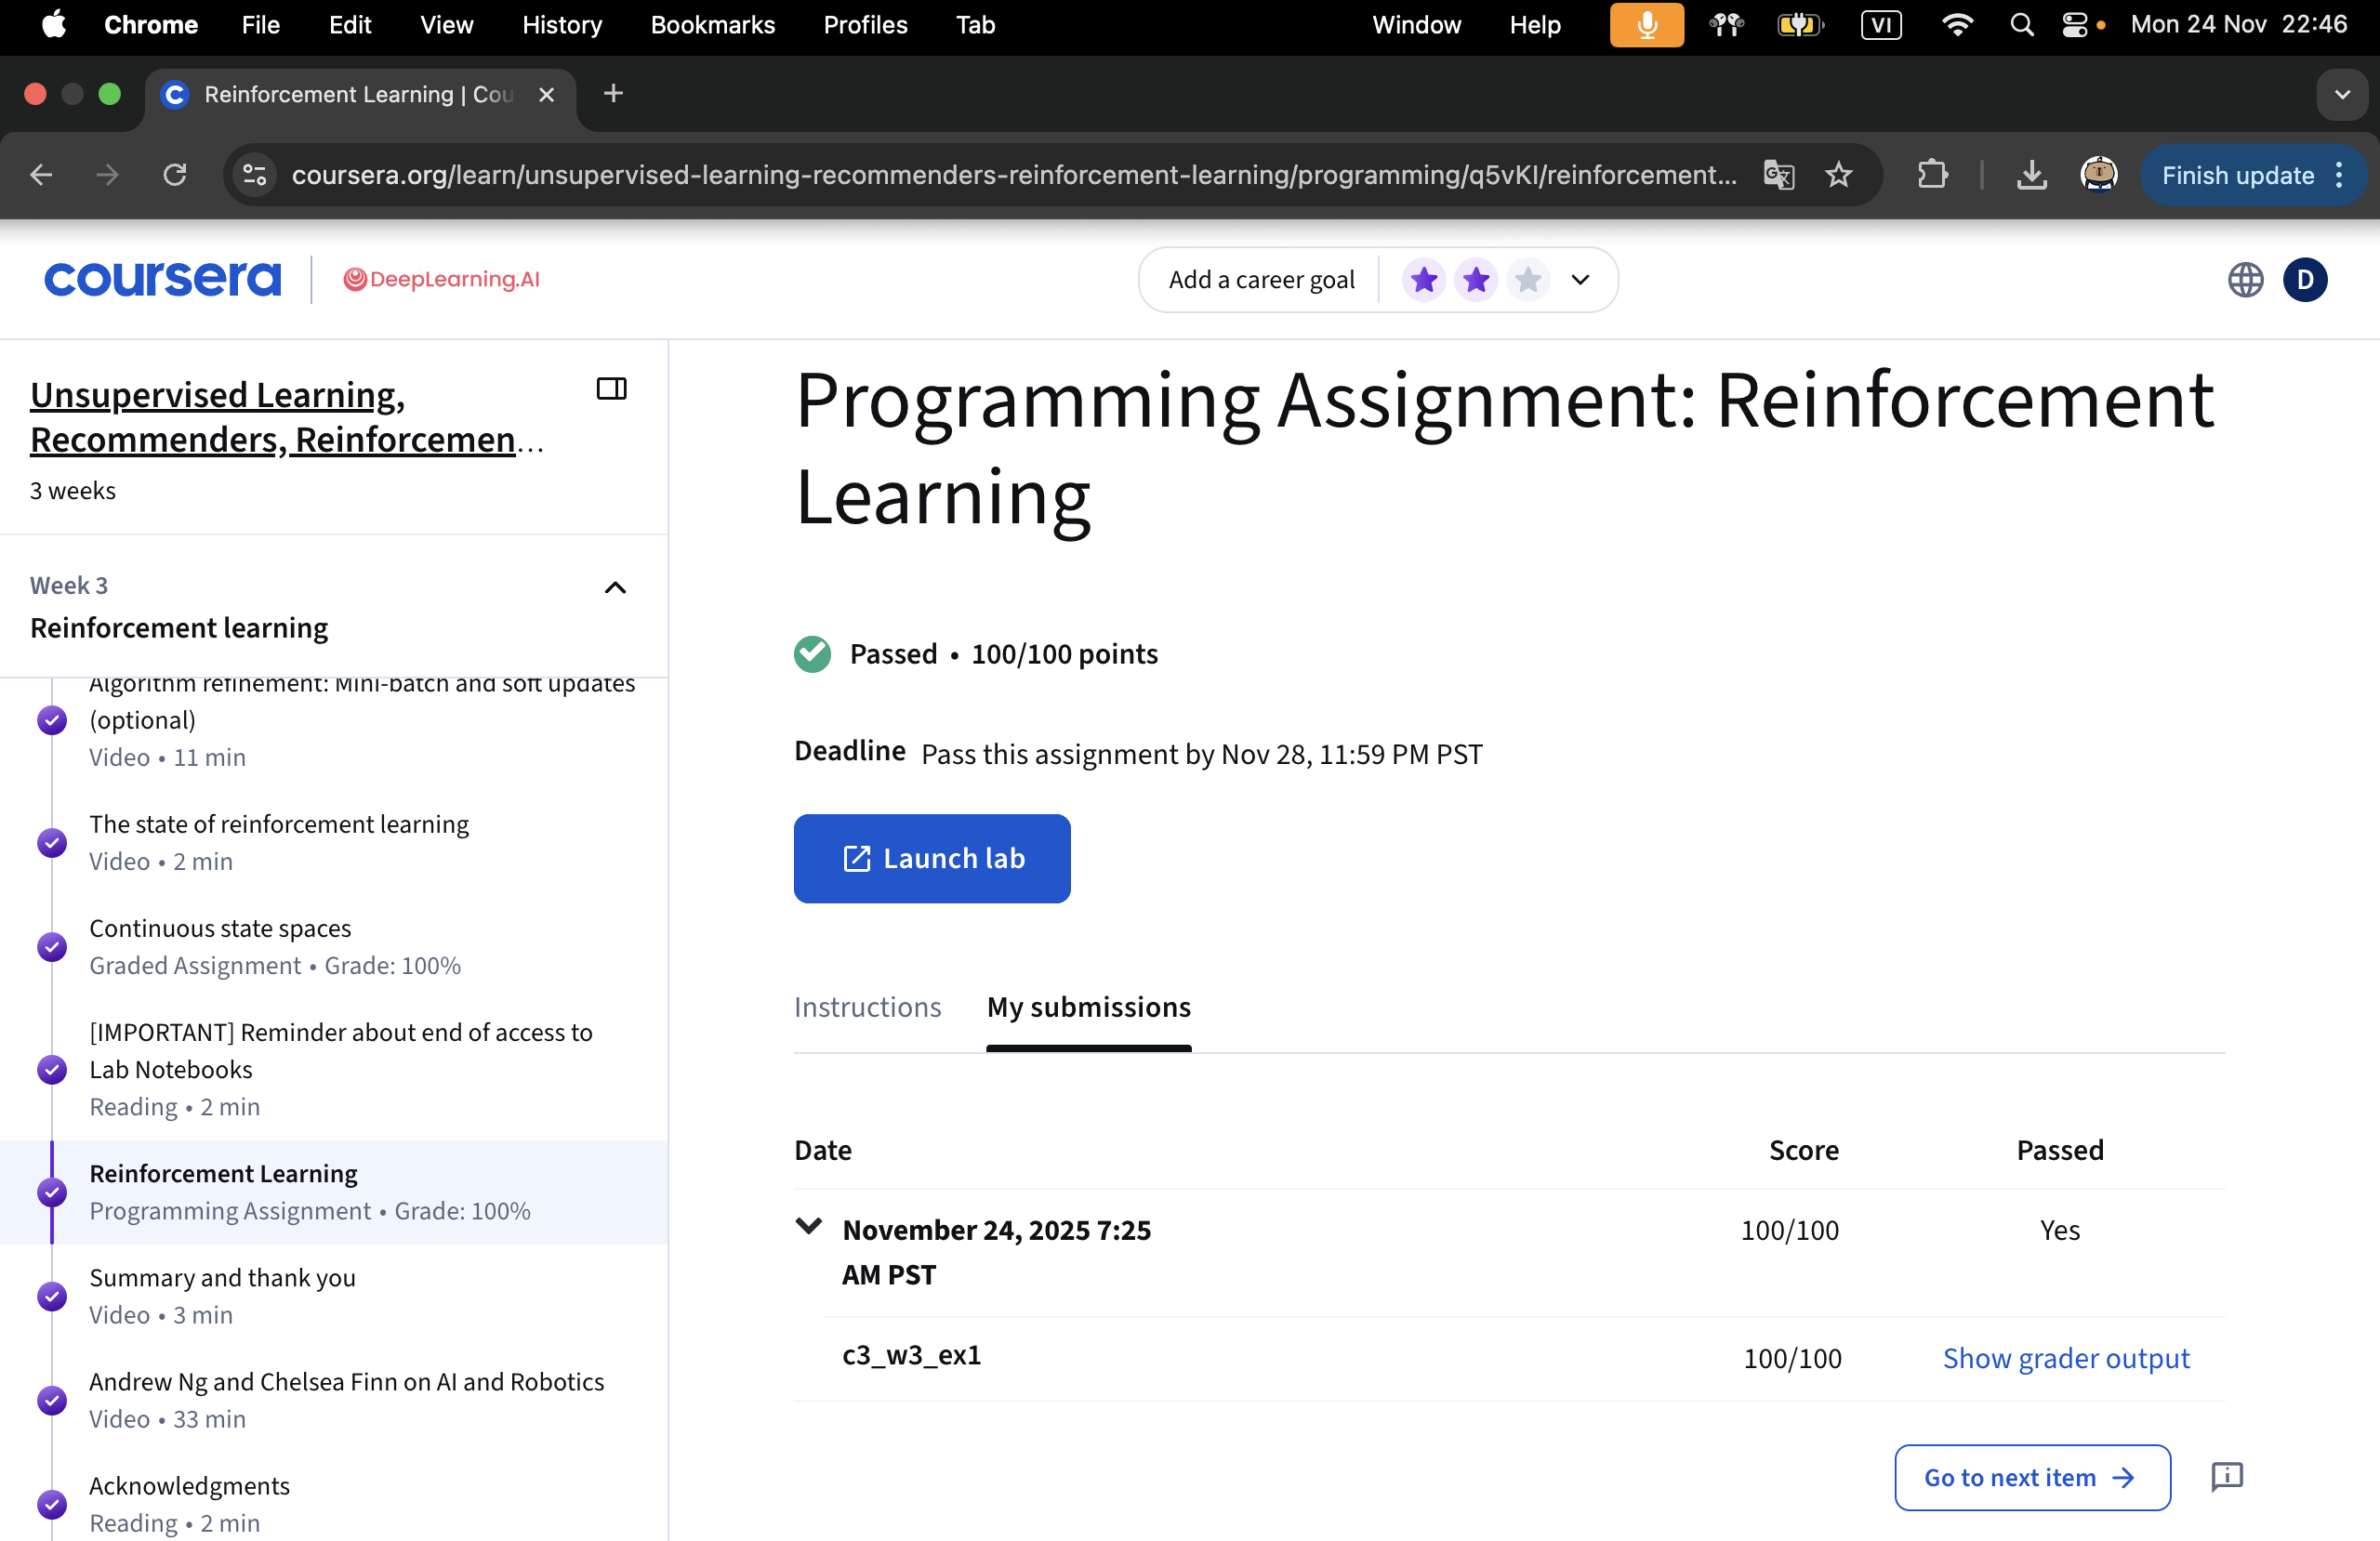
\includegraphics[scale=0.25]{Image/c3_w3_q4.png}
    \caption{Completed Programming Assignment (Reinforcement Learning)}
\end{figure}

\subsection{Certificate for Completion}
\begin{figure}[H]
    \centering
    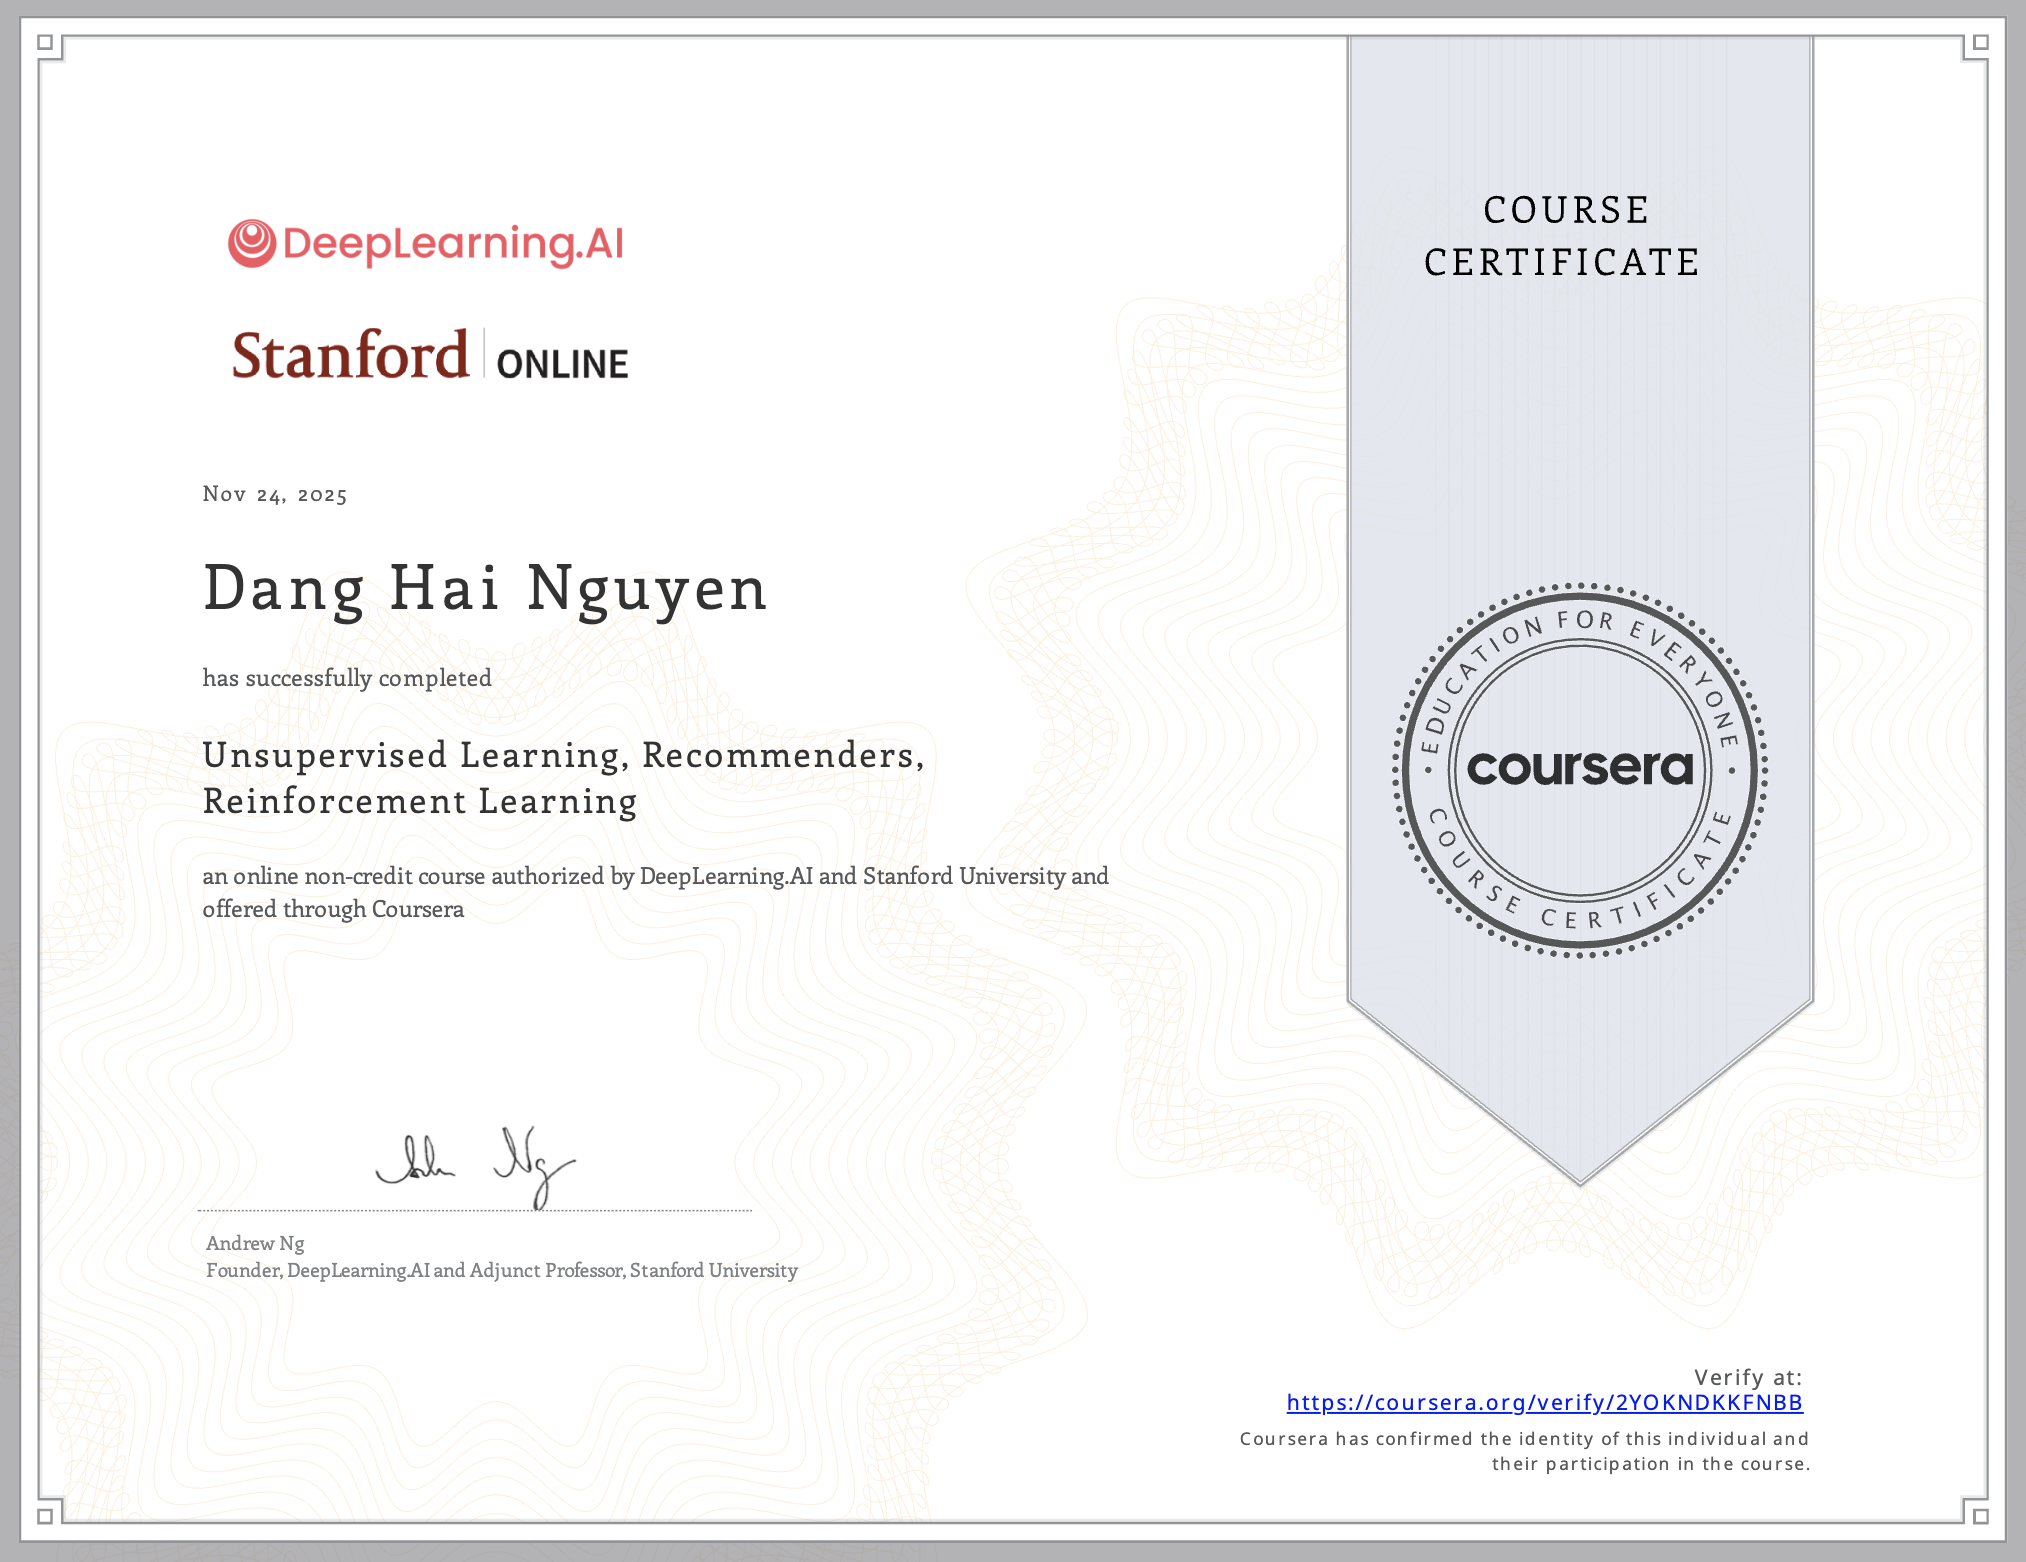
\includegraphics[scale=0.35]{Image/c3_certi.png}
    \caption{Certificate of completion for the course \textit{Unsupervised Learning, Recommenders, and Reinforcement Learning}.}
\end{figure}



%----------------------------------------
% Conclusion Section
%----------------------------------------

\section{Conclusion: A Comprehensive Journey into Machine Learning}

\indent\indent The completion of the \textit{Coursera Machine Learning Specialization} has been a transformative educational experience. This three-course program provided a comprehensive and brilliantly structured journey, starting from the foundational mathematics of supervised learning and culminating in an exploration of advanced, state-of-the-art concepts.

The specialization began by building a solid foundation in \textbf{Supervised Learning}, demystifying the core mechanics of regression and classification. It then progressed to \textbf{Advanced Learning Algorithms}, where I gained the practical skills to build and train powerful neural networks and learned indispensable, real-world methodologies for diagnosing and improving model performance. The final course, \textbf{Unsupervised Learning, Recommenders, and Reinforcement Learning}, expanded my perspective beyond labeled data, introducing me to the exciting possibilities of discovering hidden patterns, building personalized systems, and training intelligent agents.

Throughout this entire curriculum, the emphasis was not just on theoretical knowledge but also on practical application. Through hands-on labs using Python, NumPy, and TensorFlow, I translated complex mathematical concepts into functional code. More importantly, I acquired a robust mental framework for approaching machine learning problems systematically—from data preparation and feature engineering to model selection, training, and evaluation.

This specialization has equipped me with a skill set that is both broad and deep, giving me the confidence to tackle real-world data challenges and pursue more advanced topics in artificial intelligence. It has been an invaluable step in my academic and professional development.

%----------------------------------------
% Certificate Section
%----------------------------------------
\newpage

\section{Certificate of Completion}

\indent\indent As the primary evidence of my achievement, I have successfully completed all required coursework, programming assignments, and quizzes for the entire three-course \textit{Machine Learning Specialization}.

The certificate is issued by Coursera in partnership with DeepLearning.AI and Stanford Online, verifying my proficiency in the topics covered throughout this report.

\subsection{Specialization Certificate Image}

\begin{figure}[H]
    \centering
    
\includegraphics[scale=0.4]{Image/course_certi.png}
    \caption{Official Certificate of Completion for the Machine Learning Specialization.}
\end{figure}

\subsection{Verifiable Certificate Link}

The certificate can be officially verified by following the URL below:

\begin{center}
\href{https://coursera.org/share/2e43f24e9accb4486a52f76b22be6ae6}{\texttt{Course Certificates Completed}}
\end{center}

% \section{List of reference}

\begin{thebibliography}{9}
\bibitem{Ref_1}
Stuart Rusell \& Peter Novig 
\emph{\href{https://drive.google.com/drive/folders/16awghF-bo4h66hyvAn6CcM7t2FeS_DJo}{Artificial Intelligence: A Modern Approach}}

\bibitem{Ref_2}
Antonio Vrbić
\emph{\href{https://hashi-puzzles.com/generator}{Hashiwokakero Puzzle Generator}}

\bibitem{Ref_3}
Alexey Ignatiev, Joao Marques-Silva, Antonio Morgado
\emph{\href{https://pysathq.github.io/docs/pysat.pdf}{PySAT documentation}}

\bibitem{Ref_4}
Alexey Ignatiev, Joao Marques-Silva, Antonio Morgado
\emph{\href{https://pysathq.github.io/docs/html/api/pb.html}{Pseudo-Boolean encodings}}

\bibitem{Ref_5}
T. Morsink
\emph{\href{https://theses.liacs.nl/pdf/2009-11TimoMorsink.pdf}{Hashiwokakero}}

\bibitem{Ref_6}
CSC14003 - Introduction to Artificial Intelligence
\emph{\href{https://drive.google.com/drive/folders/1VP8CAJl8wAZw6Yo_AoGdu-l4O0LVzH3-}{Project 02: Hashiwokakero}}

\end{thebibliography}



\end{document}